%% ----------------------------------------------------------------
%% Thesis.tex -- MAIN FILE (the one that you compile with LaTeX)
%% ---------------------------------------------------------------- 

% Set up the document
\documentclass[a4paper, 11pt, oneside]{Thesis}	% Use the "Thesis" style, based on the ECS Thesis style by Steve Gunn
\graphicspath{{Figures/}}	% Location of the graphics files (set up for graphics to be in PDF format)

% Include any extra LaTeX packages required
\usepackage[square, numbers, comma, sort&compress]{natbib}	% Use the "Natbib" style for the references in the Bibliography
\usepackage{verbatim}	% Needed for the "comment" environment to make LaTeX comments
\usepackage{vector}	% Allows "\bvec{}" and "\buvec{}" for "blackboard" style bold vectors in maths
\hypersetup{urlcolor=blue, colorlinks=true}	% Colours hyperlinks in blue, but this can be distracting if there are many links.
\usepackage{multirow}
\usepackage{bigstrut}
\usepackage{enumerate}
\usepackage{tabulary}
\usepackage{tabularx}
\usepackage{array}
\usepackage{rotate}
\usepackage{tikz}
\usetikzlibrary{%
   arrows,%
   shapes.misc,%
   shapes.arrows,%
   chains,%
   matrix,%
   positioning,%
   scopes,%
   decorations.pathmorphing,%
   shadows%
}
%\usepackage[bottom]{footmisc}

%% ----------------------------------------------------------------
\begin{document}
\mainmatter	% Begin Roman style (i, ii, iii, iv...) page numbering

% Set up the Title Page
\title	{The Determination of the Basis of HLA Class I Associated Protection in HTLV-I Infection}
\authors	{\texorpdfstring
		{\href{http://www1.imperial.ac.uk/medicine/people/aidan.macnamara/}{Aidan MacNamara}}
		{Aidan MacNamara}
		}
\addresses	{\groupname\\\deptname\\\univname}
\date		{\today}
\subject	{}
\keywords	{}

\maketitle
%% ----------------------------------------------------------------

\setstretch{1.3}	% It is better to have smaller font and larger line spacing than the other way round

% Define the page headers using the FancyHdr package and set up for one-sided printing
\fancyhead{}	% Clears all page headers and footers
\rhead{\thepage}	% Sets the right side header to show the page number
\lhead{}	% Clears the left side page header

\pagestyle{fancy}	% Finally, use the "fancy" page style to implement the FancyHdr headers

%% ----------------------------------------------------------------
% Declaration Page required for the Thesis, your institution may give you a different text to place here
\Declaration{

\addtocontents{toc}{\vspace{1em}}	% Add a gap in the Contents, for aesthetics

I, Aidan MacNamara, declare that this thesis titled, `The Determination of the Basis of HLA Class I Associated Protection in HTLV-I Infection' and the work presented in it are my own. I confirm that:

\begin{itemize} 
\item[\tiny{$\blacksquare$}] This work was done wholly or mainly while in candidature for a research degree at this University.
 
\item[\tiny{$\blacksquare$}] Where any part of this thesis has previously been submitted for a degree or any other qualification at this University or any other institution, this has been clearly stated.
 
\item[\tiny{$\blacksquare$}] Where I have consulted the published work of others, this is always clearly attributed.
 
\item[\tiny{$\blacksquare$}] Where I have quoted from the work of others, the source is always given. With the exception of such quotations, this thesis is entirely my own work.
 
\item[\tiny{$\blacksquare$}] I have acknowledged all main sources of help.
 
\item[\tiny{$\blacksquare$}] Where the thesis is based on work done by myself jointly with others, I have made clear exactly what was done by others and what I have contributed myself.
\\
\end{itemize}
 
 
Signed:\\
\rule[1em]{25em}{0.5pt}	% This prints a line for the signature
 
Date:\\
\rule[1em]{25em}{0.5pt}	% This prints a line to write the date
}
\clearpage	% Declaration ended, now start a new page

%% ----------------------------------------------------------------
% The "Funny Quote Page"
\pagestyle{empty}	% No headers or footers for the following pages

\null\vfill
% Now comes the "Funny Quote", written in italics
\textit{``Satan delights equally in statistics and in quoting scripture...''}

\begin{flushright}
H. G. Wells
\end{flushright}

\vfill\vfill\vfill\vfill\vfill\vfill\null
\clearpage	% Funny Quote page ended, start a new page
%% ----------------------------------------------------------------

% The Abstract Page
\addtotoc{Abstract}	% Add the "Abstract" page entry to the Contents
\abstract{
\addtocontents{toc}{\vspace{1em}}	% Add a gap in the Contents, for aesthetics

\emph{Aim}

The aim of this work was to investigate what constitutes a protective cellular immune response to HTLV-I infection, focusing on understanding the relationship between HLA class I and the outcome of infection. Initially, we conducted an analysis of our patient cohort to identify robust associations between HLA class I type and infection outcome. We then identified and optimized the most accurate epitope prediction software and applied these techniques to identify the constituents of a protective HLA class I restricted response. In related projects, we identified viral factors that impact on the efficiency of the CD8$^+$ T cell response and also investigated the role of KIR:HLA genotype in the outcome of HTLV-I infection.

%The aim of this work was to investigate what constitutes a protective cellular immune response to HTLV-I infection, with a particular focus on understanding the relationship between HLA class I and the outcome of infection. Examining the CD8$^+$ T cell response to HTLV-I, we conducted a rigorous analysis of our patient cohort to identify robust associations between HLA class I type and the outcome of infection (proviral load or disease status). We then identified and optimised the most accurate epitope prediction software and applied these techniques to analyse our patient database, in order to identify the constituents of a protective HLA class I restricted response. These predictions were then then verified and tested experimentally in collaboration. In related projects, we identified viral factors that impact on the efficiency of the CD8$^+$ T cell response and also investigated the role of KIR:HLA genotype in the outcome of HTLV-I infection.

\emph{Results}

We produced a more accurate method of epitope prediction that we call Metaserver. This method was used to predict HTLV-I epitopes that bind to the HLA class I alleles of our patient cohort. We then developed a statistical method that demonstrated targeting the HTLV-I protein HBZ is beneficial in terms of disease status and proviral load. In the related analysis of the CD8$^+$ T cell response to HTLV-I infected cells, we produced a model measuring the lysis of infected cells as a function of antigen expression and showed a positive relationship between antigen expression and lysis efficiency. For our analysis of KIR genotype, we found no relationship between KIR:HLA interactions and disease status or proviral load in HTLV-I infection.

%Following a stringent analysis of currently available epitope prediction software, we produced a more accurate method of epitope prediction that we call Metaserver. This method was used to predict HTLV-I epitopes that bind to the HLA class I alleles of our patient cohort. We then developed a novel statistical method that demonstrated targeting the HTLV-I protein HBZ is beneficial in terms of disease status and proviral load. In the related analysis of the CD8$^+$ T cell response to HTLV-I infected cells, we produced a model measuring the lysis of infected cells as a function of antigen expression and showed a positive relationship between antigen expression and lysis efficiency. Finally, for our analysis of KIR genotype, we found no relationship between KIR:HLA interactions and disease status or proviral load in HTLV-I infection.

\emph{Conclusion}

We conclude that CD8$^+$ T cells play a central role in the control of HTLV-I and that CD8$^+$ cells specific to HBZ, not the immunodominant protein Tax, are the most effective. We suggest that HBZ plays a central role in HTLV-I persistence. The statistical method we used to quantify the specificity of HLA class I binding to viral epitopes is applicable across all pathogens, even where data are sparse.

%We conclude that CD8$^+$ T cells play a central role in the control of HTLV-I and that CD8$^+$ cells specific to HBZ, not the immunodominant protein Tax, are the most effective. We suggest that HBZ plays a central role in HTLV-I persistence. The statistical method we used to quantify the specificity of HLA class I binding to viral epitopes is applicable across all pathogens, even where data are sparse. We also found that antigen density was a determinant of CD8$^+$ lysis efficiency. Finally, we found no evidence that NK cells play a major role in determining the outcome to HTLV-I infection.
 
%showed that previously defined beneficial alleles (A*02 and Cw*08) strongly bind to epitopes from the HTLV-I protein HBZ, compared to the defined detrimental allele (B*54). We also showed that asymptomatic carriers possess HLA class I alleles that bind to HBZ epitopes more strongly than HAM/TSP individuals' HLA class I repertoire.

%Using a patient cohort of 432 HTLV-I infected individuals, 202 asymptomatic and 232 showing symptoms of disease, we initially conducted a rigorous analysis to identify robust associations betweem HLA class I type and the outcome of infection. We then identified and optimised the most accurate epitope prediction software available to test hypotheses about HLA class I type and the HTLV-I viral epitopes that they present to the host CD8$^+$ population. Finally the predictions of this work were tested in collaboration with experimentalists.

}

\clearpage	% Abstract ended, start a new page
%% ----------------------------------------------------------------

\setstretch{1.3}	% Reset the line-spacing to 1.3 for body text (if it has changed)

% The Acknowledgements page, for thanking everyone
\acknowledgements{
\addtocontents{toc}{\vspace{1em}}	% Add a gap in the Contents, for aesthetics

I would like to thank my supervisor, Becca Asquith, for her advice, time, support and encouragement throughout my PhD and for producing a great environment for learning. I would also like to thank Charles Bangham for his help and support and his infectious enthusiasm for HTLV-I research and science in general.

Many thanks to Ulrich Kadolsky. As a computational biologist, with the emphasis on biology, I was fortunate to be sitting next to a real computer scientist, or else everything would have taken a good deal longer. I would also like to thank my collaborators within the Department of Immunology, namely Tarek Kattan and Aileen Rowan. It was very enjoyable working together to produce research that combined experimental and theoeretical approaches. I would also like to thank Graham Taylor and Silva Hilburn for their help with my research and everyone in the department for their general help and support.

I am grateful to the Wellcome Trust for funding this work.

Finally, I would like to thank Jaydee, Noah and my family for their patience with all those hours spent in front of the computer!

}
\clearpage	% End of the Acknowledgements
%% ----------------------------------------------------------------

\pagestyle{fancy}	% The page style headers have been "empty" all this time, now use the "fancy" headers as defined before to bring them back

%% ----------------------------------------------------------------
\lhead{\emph{Contents}}	% Set the left side page header to "Contents"
\tableofcontents	% Write out the Table of Contents

%% ----------------------------------------------------------------
\lhead{\emph{List of Figures}}	% Set the left side page header to "List if Figures"
\listoffigures	% Write out the List of Figures

%% ----------------------------------------------------------------
\lhead{\emph{List of Tables}}	% Set the left side page header to "List of Tables"
\listoftables	% Write out the List of Tables

%% ----------------------------------------------------------------
\setstretch{1.5}	% Set the line spacing to 1.5, this makes the following tables easier to read
\clearpage	% Start a new page
\lhead{\emph{Abbreviations}}	% Set the left side page header to "Abbreviations"
\listofsymbols{ll}	% Include a list of Abbreviations (a table of two columns)
{
% \textbf{Acronym} & \textbf{W}hat (it) \textbf{S}tands \textbf{F}or \\
\textbf{AC} & \textbf{A}symptomatic \textbf{C}arriers \\
\textbf{ATL} & \textbf{A}dult \textbf{T}-cell \textbf{L}eukaemia/Lymphoma \\
\textbf{AUC} & \textbf{A}rea \textbf{U}nder \textbf{C}urve \\
\textbf{CNS} & \textbf{C}entral \textbf{N}ervous \textbf{S}ystem \\
\textbf{CSF} & \textbf{C}erebrospinal \textbf{F}luid \\
\textbf{CTL} & \textbf{C}ytotoxic \textbf{T} \textbf{L}ymphocyte \\
\textbf{dsDNA} & \textbf{D}ouble \textbf{S}tranded \textbf{D}eoxy\textbf{r}ibo\textbf{n}ucleic acid \\
\textbf{ELISpot} & \textbf{E}nzyme-\textbf{L}inked Immuno\textbf{spot} Assay \\
\textbf{FACS} & \textbf{F}luoresence \textbf{A}ctivated \textbf{C}ell \textbf{S}orting \\
\textbf{FCS} & \textbf{F}oetal \textbf{C}alf \textbf{S}erum \\
\textbf{HAM/TSP} & \textbf{H}TLV-I \textbf{A}ssociated \textbf{M}yelopathy / \\ 
& \textbf{T}ropical \textbf{S}pastic \textbf{P}araparesis \\
\textbf{HBV} & \textbf{H}epatitis \textbf{B} \textbf{V}irus \\ 
\textbf{HBZ} & \textbf{H}TLV-I \textbf{bZ}IP-Factor \\
\textbf{HCV} & \textbf{H}epatitis \textbf{C} \textbf{V}irus \\
\textbf{HIV} & \textbf{H}uman \textbf{I}mmunodeficiency \textbf{V}irus \\
\textbf{HLA} & \textbf{H}uman \textbf{L}eucocyte \textbf{A}ntigen \\
\textbf{IFN} & \textbf{I}nter\textbf{f}ero\textbf{n} \\
\textbf{Ig} & \textbf{I}mmuno\textbf{g}lobulin \\
\textbf{KIR} & \textbf{K}iller Cell \textbf{I}munnoglobulin-like \textbf{R}eceptor \\
\textbf{LTR} & \textbf{L}ong \textbf{T}erminal \textbf{R}epeat \\
\textbf{MHC} & \textbf{M}ajor \textbf{H}istocompatibility \textbf{C}omplex \\ 
\textbf{ORF} & \textbf{O}pen \textbf{R}eading \textbf{F}rame \\
\textbf{PBMC} & \textbf{P}eripheral \textbf{B}lood \textbf{M}ononuclear \textbf{C}ells \\
\textbf{SD} & \textbf{S}tandard \textbf{D}eviation \\
\textbf{TCR} & \textbf{T}-\textbf{C}ell \textbf{R}eceptor \\
\textbf{TNF} & \textbf{T}umour \textbf{N}ecrosis \textbf{F}actor \\
\textbf{WHO} & \textbf{W}orld \textbf{H}ealth \textbf{O}rganisation \\

% TO ADD 

}

%% ----------------------------------------------------------------
%\clearpage	% Start a new page
%\lhead{\emph{Physical Constants}}	% Set the left side page header to "Physical Constants"
%\listofconstants{lrcl}	% Include a list of Physical Constants (a four column table)
%{
% Constant Name & Symbol & = & Constant Value (with units) \\
%Speed of Light & $c$ & $=$ & $2.997\ 924\ 58\times10^{8}\ \mbox{ms}^{-\mbox{s}}$ (exact)\\
%}

%% ----------------------------------------------------------------
\clearpage	%Start a new page
\lhead{\emph{Symbols}}	% Set the left side page header to "Symbols"
\listofnomenclature{lll}	% Include a list of Symbols (a three column table)
{
\textbf{Symbol} & \textbf{Name} & \textbf{Unit} \\
$c$ & Rate of increase of tax expression & Tax$^+$CD4$^+$ / 24hrs \\
$c_1$ & Rate of increase of Tax\superscript{low} expression & Tax\superscript{low}CD4$^+$ / 24hrs \\
$c_2$ & Rate of increase of Tax\superscript{high} expression & Tax\superscript{high}CD4$^+$ / 24hrs \\
$y$ & Proportion of Tax\superscript{low}CD4$^+$ cells & \%Tax\superscript{low}CD4$^+$cells \\
$w$ & Proportion of Tax\superscript{high}CD4$^+$ cells & \%Tax\superscript{high}CD4$^+$cells \\
$\epsilon$ & Rate of killing of Tax$^+$CD4$^+$ cells per CD8$^+$ & Tax$^+$CD4$^+$ / CD8$^+$ / 24hrs \\
$\epsilon$\superscript{low} & Rate of killing of Tax\superscript{low}CD4$^+$ cells per CD8$^+$ & Tax\superscript{low}CD4$^+$ / CD8$^+$ / 24hrs \\
$\epsilon$\superscript{high} & Rate of killing of Tax\superscript{high}CD4$^+$ cells per CD8$^+$ & Tax\superscript{high}CD4$^+$ / CD8$^+$ / 24hrs \\

}

%% ----------------------------------------------------------------
% End of the preamble, contents and lists of things
% Begin the Dedication page

\setstretch{1.3}	% Return the line spacing back to 1.3

%\pagestyle{empty}	% Page style needs to be empty for this page
%\dedicatory{For/Dedicated to/To my\ldots}

\addtocontents{toc}{\vspace{2em}}	% Add a gap in the Contents, for aesthetics

%% ----------------------------------------------------------------
%\mainmatter	% Begin normal, numeric (1,2,3...) page numbering
\pagestyle{fancy}	% Return the page headers back to the "fancy" style

% Include the chapters of the thesis, as separate files
% Just uncomment the lines as you write the chapters

% Chapter 1

\chapter{Aim and Overview} % Write in your own chapter title
\label{Chapter1}
\lhead{Chapter 1. \emph{Aim and Overview}} % Write in your own chapter title to set the page header

\section{Introduction}

Host genetic factors, including the HLA class I genotype, are major determinants of susceptibility to infectious disease in humans. However, it is currently a difficult task to demonstrate a direct link between the host immune response and the outcome of viral infections in either human or animal populations \citep{Jeffery1999}. Human T-lymphotropic virus-I (HTLV-I) is a persistent retrovirus that infects 10-20 million people worldwide. The virus is endemic in the Caribbean, Japan and parts of Africa. Most infected people remain healthy, but 1-2\% develop a progressive paralytic myelopathy (HTLV-I associated myelopathy/tropical spastic paraparesis; HAM/TSP) and a further 2-3\% develop an aggressive T cell leukaemia/lymphoma. The reasons for these different outcomes is unknown. What is known is that the risk of HAM/TSP is determined, in part, by the host's HLA class I alleles. 

Cells that have become infected with a virus are recognized by the host immune system because they display fragments of the pathogen bound to HLA class I molecules on the infected cell surface. Different people have a diverse range of shapes that make up the HLA class I molecules, owing to their different alleles. Thus, the molecules bind to different parts of the pathogen proteome and present this peptide (or epitope in this context) to CD8$^+$ cytotoxic T lymphocytes (CTLs). Once CTLs recognize the HLA-peptide complex, they are capable of destroying the infected cell by the release of lytic granules containing cytotoxic effector proteins. This results in the destruction of the target cell by apoptosis. An effective CTL response has been shown to confer protection against viral infection, such as HIV \citep{Ngandu2007} and HTLV-I \citep{Bangham2005}. The effectiveness of the response varies between individuals and part of this variation is thought to be due to differences in the host genotype.

The ultimate aim of the project is to increase our understanding of why some HLA class I molecules are better than others at eliciting a more effective immune response. This would increase our knowledge of a key part of the immune system and specifically the design and implementation of improved vaccines.

\section{PhD Design}

\begin{center}
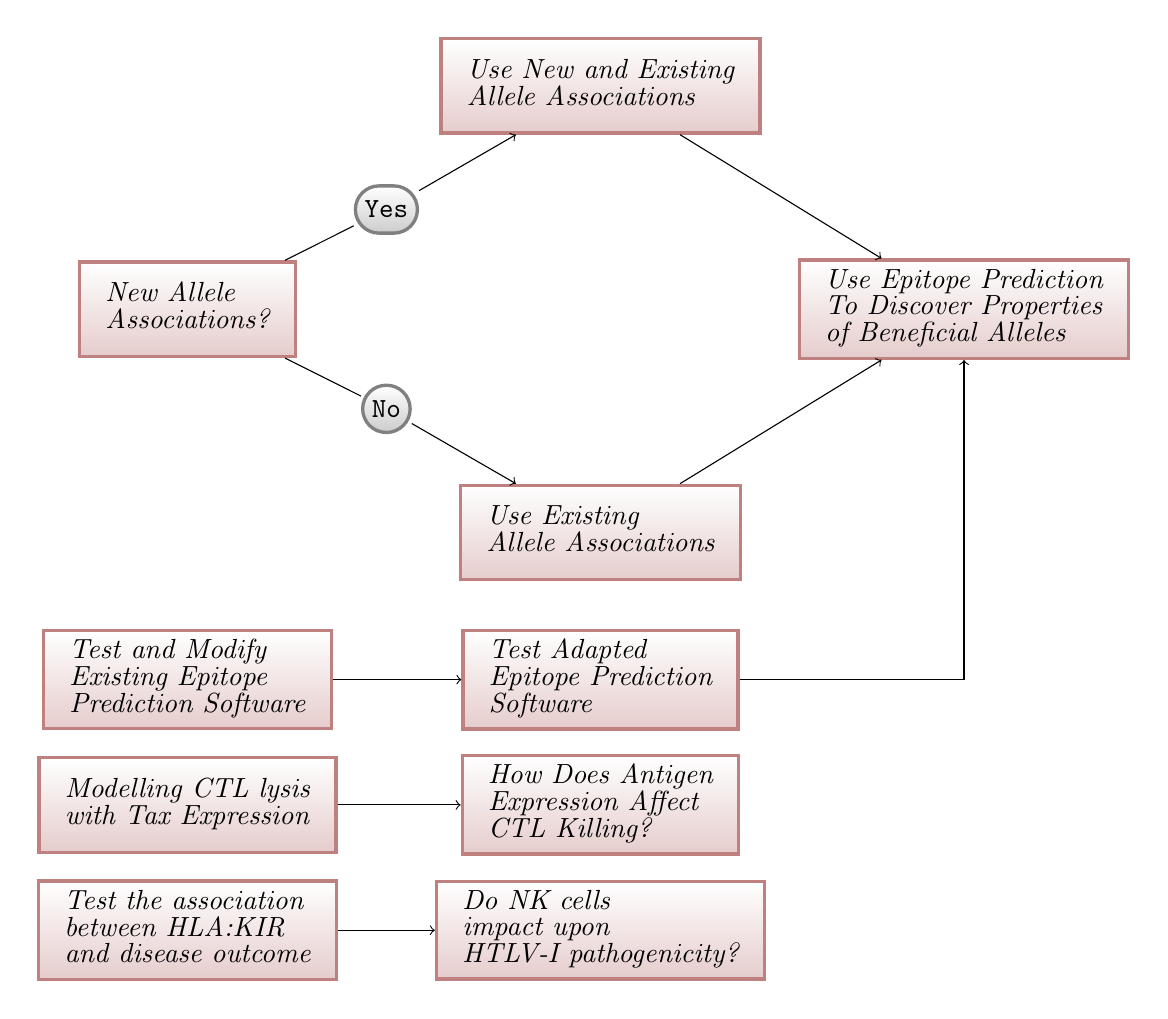
\begin{tikzpicture}[nonterminal/.style={
	rectangle,
	minimum size=12mm,
	very thick,
	draw=red!50!black!50, 
	top color=white, 
	bottom color=red!50!black!20,
	font=\itshape
	},terminal/.style={
	rectangle,minimum size=6mm,rounded corners=3mm,
	very thick,draw=black!50,
	top color=white,bottom color=black!20,
	font=\ttfamily
	},point/.style={
	coordinate,thick,draw=black!50
	}
%	Need to check these with chain	
%	 ,tip/.style={
%	->,shorten >=1pt
%	},every join/.style={
%	rounded corners
%	},hv path/.style={
%	to path={-| (\tikztotarget)}
%	},vh path/.style={
%	to path={|- (\tikztotarget)}
%	}
]

\matrix[row sep=3mm,column sep=2mm] {
% First row
& & \node (atom1) [nonterminal,yshift=9.5mm] {{\renewcommand{\arraystretch}{0.75}\begin{tabular}{l} Use New and Existing \\ Allele Associations \end{tabular}}}; & & \\
& \node (yes1) [terminal] {Yes}; & & & \\
% Second row
\node (atom2) [nonterminal] {{\renewcommand{\arraystretch}{0.75}\begin{tabular}{l} New Allele \\ Associations? \end{tabular}}}; & & & & \node (atom3) [nonterminal] {{\renewcommand{\arraystretch}{0.75}\begin{tabular}{l} Use Epitope Prediction \\ To Discover Properties \\ of Beneficial Alleles \end{tabular}}}; \\
& \node (no1) [terminal] {No}; & & & \\
% Third row
& & \node (atom4) [nonterminal,yshift=-9.5mm] {{\renewcommand{\arraystretch}{0.75}\begin{tabular}{l} Use Existing \\ Allele Associations \end{tabular}}}; & & \\
\\

\node (atom5) [nonterminal] {{\renewcommand{\arraystretch}{0.75}\begin{tabular}{l} Test and Modify \\ Existing Epitope \\ Prediction Software \end{tabular}}}; & & \node (atom6) [nonterminal] {{\renewcommand{\arraystretch}{0.75}\begin{tabular}{l} Test Adapted \\ Epitope Prediction \\ Software \end{tabular}}}; & & \node (pos1) [point] {.};\\
\node (atom7) [nonterminal] {{\renewcommand{\arraystretch}{0.75}\begin{tabular}{l} Modelling CTL lysis \\ with Tax Expression \end{tabular}}}; & & \node (atom8) [nonterminal] {{\renewcommand{\arraystretch}{0.75}\begin{tabular}{l} How Does Antigen \\ Expression Affect \\ CTL Killing? \end{tabular}}}; & & \\
\node (atom9) [nonterminal] {{\renewcommand{\arraystretch}{0.75}\begin{tabular}{l} Test the association \\ between HLA:KIR \\ and disease outcome \end{tabular}}}; & & \node (atom10) [nonterminal] {{\renewcommand{\arraystretch}{0.75}\begin{tabular}{l} Do NK cells \\ impact upon \\ HTLV-I pathogenicity? \end{tabular}}}; & & \\
};

%	chain not working, try again if you have time

\path	(atom2)	edge[-] (yes1)
	(atom2) edge[-] (no1)
	(yes1) 	edge[->] (atom1)
	(no1) 	edge[->] (atom4)
	(atom1) edge[->] (atom3)
	(atom4) edge[->] (atom3);
\path	(atom5) edge[->] (atom6)
	(atom6) edge[-] (pos1)
	(pos1) 	edge[->] (atom3);
\path	(atom7) edge[->] (atom8);
\path	(atom9) edge[->] (atom10);

\end{tikzpicture}
\end{center}

\subsection{Identifying Alleles Associated with Risk or Prevention in HTLV-I Infection}\label{chapter1/AlleleAssoc}

The work of Jeffery \emph{et al.} \citep{Jeffery1999} produced evidence that a number of HLA class I alleles are associated with either disease risk or protection in HTLV-I infection. Added to this, results showing that class I heterozygosity is associated with significantly lower proviral loads \citep{Jeffery2000} would suggest that the protective effect of the HLA haplotype extends to a range of alleles.

Hence, my initial task was to reanalyze a database of individuals from Kagoshima, Japan, who had been infected with HTLV-I and displayed symptoms of HAM/TSP (see \sref{chapter2/HAM/TSP}: HAM/TSP description) or remained asymptomatic. \cref{Chapter3} details the progression of this work.

\subsection{Epitope Prediction}\label{chapter1/EpPred}

There are relatively few experimentally confirmed HTLV-I epitopes for HLA class I alleles compared to HIV. Therefore, in order to test the protective properties of specific HLA class I alleles, it was necessary to use epitope prediction software to predict what epitopes these alleles bind to. The aim of this section was to test the accuracy and predictive power of a number of web-based prediction servers. The starting point was NetCTL v1.2, an integrated web-based prediction method that used information pertaining to proteasomal cleavage, TAP and HLA-peptide binding in epitope prediction. We tested and modified this method, in conjunction with other epitope prediction software, to produce a novel method of epitope prediction that we used for the purpose of discovering the HTLV-I epitopes of ``beneficial'' or ``detrimental'' alleles. The details of this work are in \cref{Chapter4}.

\subsection{The Properties of HLA class I Alleles Associated with Disease Outcome}

Combining the two strands of research, \sref{chapter1/AlleleAssoc} and \sref{chapter1/EpPred}, gave us the ability to predict HTLV-I epitopes for each of the HLA class I alleles contained within the Kagoshima database. Hence, we were able to test what properties of these epitopes were associated with disease risk and proviral load. For instance, we asked the question, ``do alleles associated with protection from disease bind to specific regions of the HTLV-I proteome?''. The details of this work are in \cref{Chapter6}.

\subsection{Modelling CTL Efficiency in Terms of Tax Expression}

In the work detailed above we analyzed the host genetic factors that determine the efficiency of the CD8$^+$ T cell response. We then extended this work to investigate the CD8$^+$ T cell response itself in terms of its properties and dynamics.

In collaboration with experimentalists within the Department of Immunology, we examined the efficiency of CTL-mediated lysis. We tested the hypothesis that the lysis of infected target cells may depend on the expression level of the viral protein Tax in the target cell. This was based on experimental data that showed target cells expressing a higher level of Tax per cell may be killed quicker by CD8$^+$ cells. The analysis consisted of a series of lytic assays, followed by the development of models of Tax expression dynamics and the rate of killing of target cells by CD8$^+$ cells. This data is shown in \cref{Chapter5}.

\subsection{HLA Class I Alleles and KIR Genotype}

One of the main roles of HLA class I molecules is to present antigen to CD8$^+$ T cells. However, HLA-peptide complexes are also recognized by natural killer (NK) cells via their killer cell immunoglobulin (Ig)-like receptors (KIRs). NK cells are critical components of the innate immune system that have direct involvement in the anti-viral immune response. Disease association studies have shown that the interaction between KIR and HLA class I can be protective or detrimental to disease progression in a number of viral infections. In \cref{Chapter7}, we tested the hypothesis that KIR-HLA interactions are predictive of disease status in HTLV-I infection.	% Aim and Overview
% Chapter 2

\chapter{Introduction} % Write in your own chapter title
\label{Chapter2}
\lhead{Chapter 2. \emph{Introduction}} % Write in your own chapter title to set the page header

One of the most important contributions to human health has been vaccination. From the success of Jenner�s and Pasteur�s vaccines against smallpox and chicken cholera, through to the global campaign for the eradication of polio and the widespread immunization against potentially fatal childhood diseases, vaccination has been a vital component of preventative health care. However, the threat of emerging diseases such as avian influenza, as well as current epidemic diseases such as HIV/AIDS, malaria and tuberculosis, has ensured that vaccine development remains a vital component of biomedical research.

One course of vaccination development that has shown recent promise is the identification and utilization of peptide epitopes that stimulate protective immunity. This technique takes advantage of the adaptive immune response to foreign proteins, such as viruses, where pieces of these proteins called epitopes are recognized by the antigen-specific receptors of the immune system (e.g. T-cell receptors, antibodies). Hence, the goal of the vaccine is to safely expose the immune system to pathogenic epitopes to induce an immune response. There are a number of challenges associated with this: identifying what the pathogenic epitopes should be, designing effective delivery of the epitopes when they are found. And increasingly, understanding the complexity of how this works.

The human T-cell lymphotropic virus type 1 (HTLV-I) was the first human retrovirus discovered and its associated diseases: ATL (Adult T-cell leukaemia/lymphoma), HAM/TSP (HTLV-I associated myelopathy/tropical spastic paraparesis) and other chronic inflammatory diseases cause considerable global morbidity and mortality. This chapter gives an overview of the pathogenesis and treatment of the virus and demonstrates the relevancy of my work to understand the basis of an effective immune response towards HTLV-I infection. Hence, a greater understanding of the targets (epitopes) of HTLV-I specific CD8$^+$ T cells may lead to a vaccine against this widespread debilitating virus.

\section{HTLV-I}

\subsection{Virology}

HTLV-I is a type C 
% morphology in negatively-stained E.M.
particle-like onco-retrovirus, and its discovery was first reported in 1980 when a retrovirus was successfully isolated from a T-lymphoblastoid cell line (HUT 102) established from a patient with a cutaneous T-cell lymphoma \citep{Poiesz1980}. This discovery was the first formal proof that human retroviruses exist and suggested their aetiological role in human cancer, a hypothesis that had been proposed decades before \citep{The1993}. The diploid genome consists of 2 identical positive single-stranded RNA molecules each of 9032 bases associated in a complex. It contains the typical retroviral genes of \gene{gag}, \gene{pol} and \gene{env}, and in addition genes encoding regulatory proteins such as \gene{tax} and \gene{rex}.

Gag comprises the structural polypeptides p15 (nucleocapsid), p19 (matrix) and p24 (capsid). Env encodes the envelope protein which is cleaved into the surface glycoprotein gp46 (SU) and the transmembrane protein p21 (TM). Pol encodes the genes for reverse transcriptase, integrase and RNaseH. The rest of the genome contains unique accessory genes in four open reading frames (ORFs) of the pX region of the viral genome, as well as a negative strand product, HTLV-I bZIP-factor (\fref{chapter2/figure2}). The regulatory proteins encoded by pX ORFs III and IV, Tax and Rex, respectively, have been extensively characterized. Tax is a \emph{trans}-acting transcriptional activator. It is of central importance in the dynamics of HTLV-I infection as it is thought to be one of the first to be expressed in the viral life cycle and is a promiscuous transcriptional transactivator. It transactivates both its own LTR and many of those of the infected host cell. It is also central to the host's immune response to the virus as it is the dominant target antigen for the CTL response \citep{Jacobson1990, Kannagi1991, Parker1992, Parker1994, Goon2004}. Rex is an essential shuttle protein required for nuclear export of unspliced and incompletely-spliced viral RNAs \citep{Heger1999}.

Open reading frames I and II are less well known. Both ORFs are alternatively spliced, producing the proteins Rof (p27\superscript{I}) and p12\superscript{I} for ORF I and Tof (p30\superscript{II}) and p13\superscript{II} for ORF II. It was thought that ORFs I and II did not significantly affect viral replication. While the expression of mRNAs for these proteins is well-documented \emph{in vitro} and \emph{ex vivo}, their detection in infected cells has remained elusive. However, a body of evidence suggests that these proteins may be essential for viral persistence. p12\superscript{I} localizes to cellular endomembranes, particularly the ER and expression in virally infected cells could result in decreased expression of MHC class I on the cell surface, thereby protecting infected cells from CTL recognition \citep{Nicot2005}. Recent findings suggest that p30\superscript{II} functions as a post-transcriptional regulator of Tax/Rex mRNA and may also modulate the expression of viral and cellular genes \citep{Nicot2005}. In the presence of Tax, p13\superscript{II} is stabilized and localizes to the nucleus. It has been reported that p13\superscript{II} induces Tax degradation and inhibits its transcriptional activity, thereby decreasing viral replication \citep{Willems2009}.

\begin{figure}[htp]
\centering
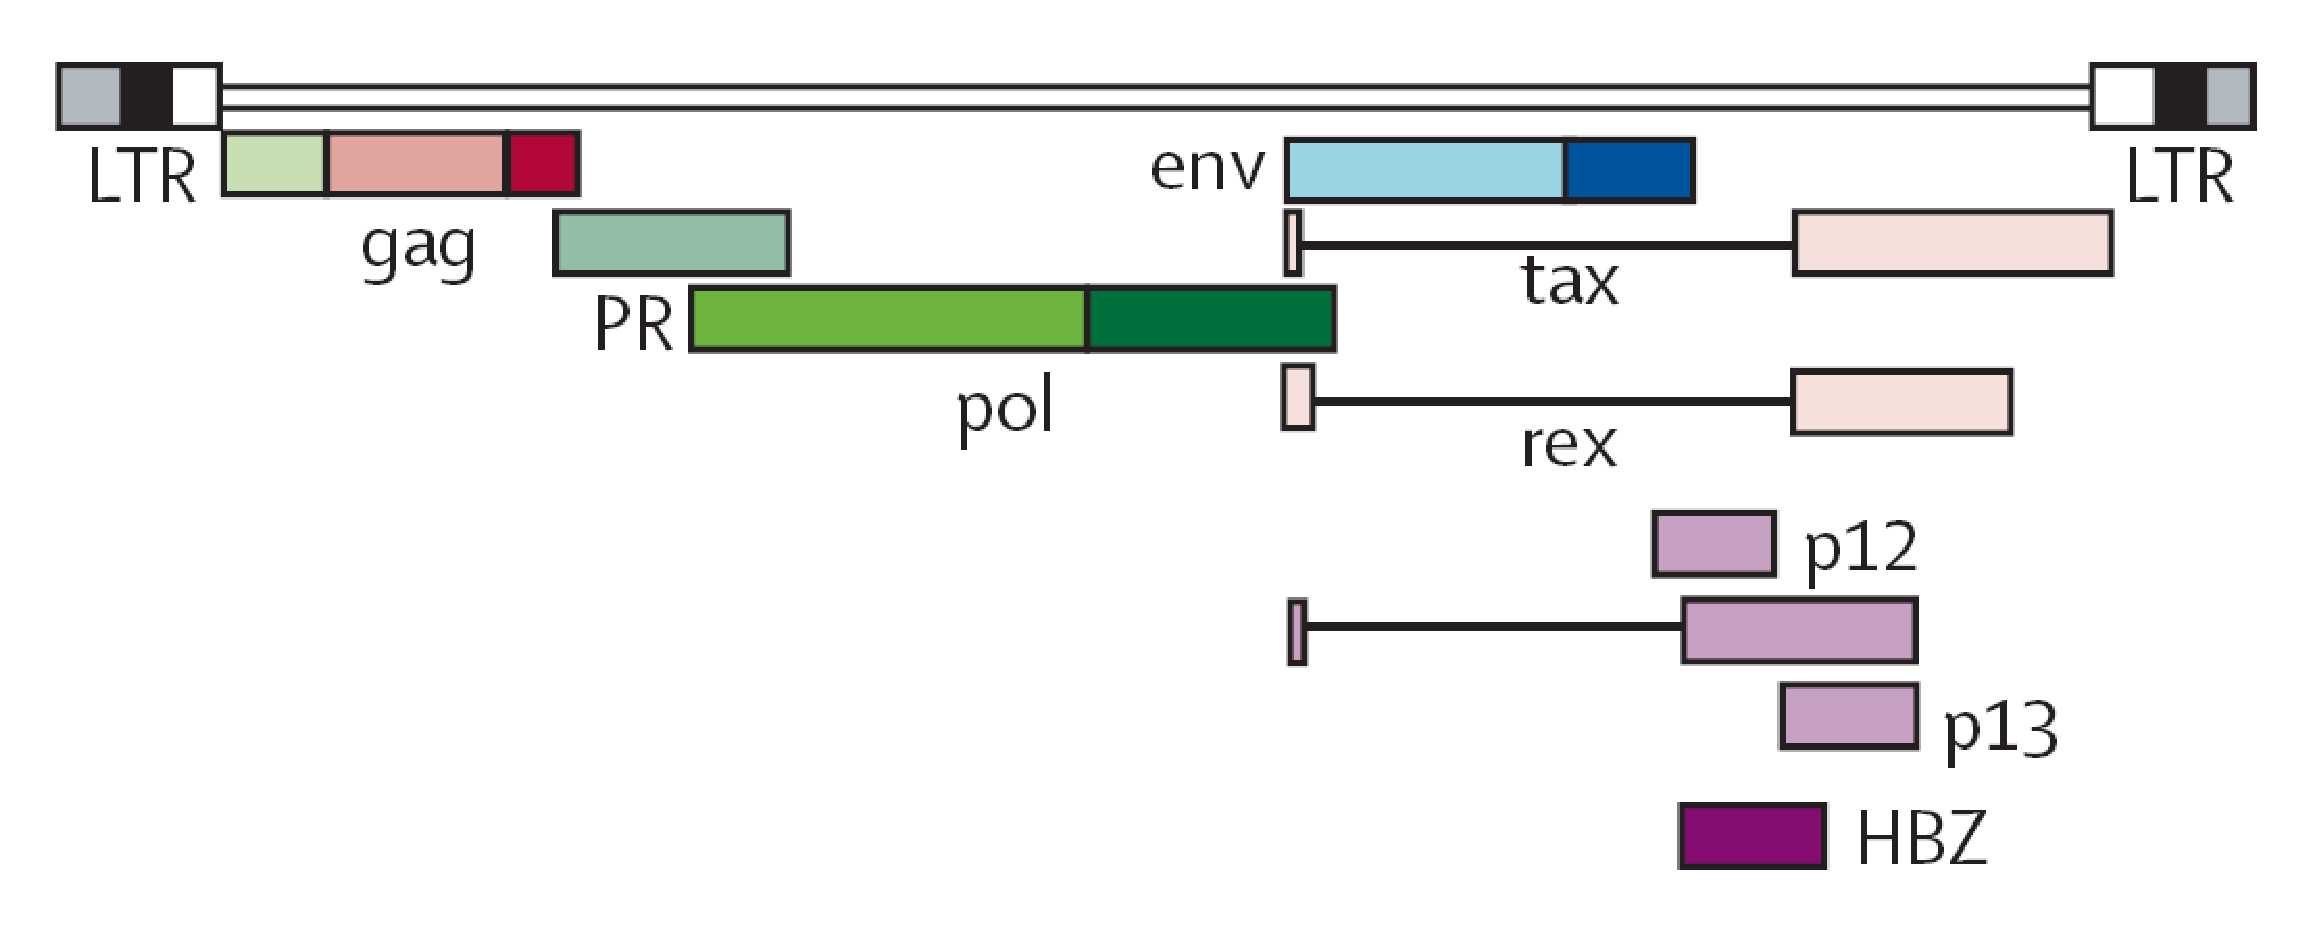
\includegraphics[width=14cm]{./Figures/chapter2/genotype}
\rule{35em}{0.5pt}
\caption[The genomic organisation of HTLV-I]{The genomic organisation of HTLV-I, taken from \citep{Verdonck2007}}
\label{chapter2/figure2}
\end{figure}

It is believed that humans have been exposed to HTLV-I for thousands of years \citep{Novak1999, Gessain2000, Vandamme2000} and HTLV-I viral DNA has been detected in Andean mummies 1,500 years old \citep{Li1999, Sonoda2000}. Even though the virus has been in contact with humans for this amount of time, HTLV-I isolates from Japan, Africa, the Caribbean Basin and the Americas show high sequence conservation (0.5 to 4\%) \citep{Gessain1993}. HTLV-I has been classified into three major lineages known as the Cosmopolitan, Central African and Melanesian groups \citep{Gessain1992, Saksena1992, Gessain1993}. There is further subdivision of the Cosmopolitan group into four subgroups based on LTR sequencing; these are the (A) Transcontinental, (B) Japanese, (C) West African and (D) North African \citep{Gasmi1994, Miura1994}. Generally, a single viral genotype is found in any one location but in Kagoshima, Southern Japan, both Cosmopolitan A (Transcontinental) and B (Japanese) coexist because of its location between Honshu Island (Cosmopolitan B) and Okinawa (Cosmopolitan A) \citep{Vidal1994a, Furukawa2000}.

The virus infects T-cells, with CD4$^+$ and CD45RO$^+$ T-lymphocytes being the main targets for infection \citep{Hanon2000a, Richardson1990}. CD8$^+$ T-cells have also been shown to act as as reservoir for the virus \emph{in vivo} \citep{Nagai2001, Hanon2000b}. HTLV-I can spread directly between lymphocytes across a specialized, virus-induced cell-cell contact - a `viral synapse' \citep{Bangham2003}. The cellular receptor for HTLV-I has not been identified, despite intensive efforts over many years. However, its presence has been demonstrated by virus-induced cell fusion experiments, leading to syncytium formation \citep{Hoshino1983, Nagy1983}. It has been mapped to chromosome 17 (17q region) \citep{Sommerfelt1988} but it is possible that this site encodes not the putative receptor but just an essential cofactor. 

\subsection{Epidemiology}

\begin{figure}[htp]
\centering
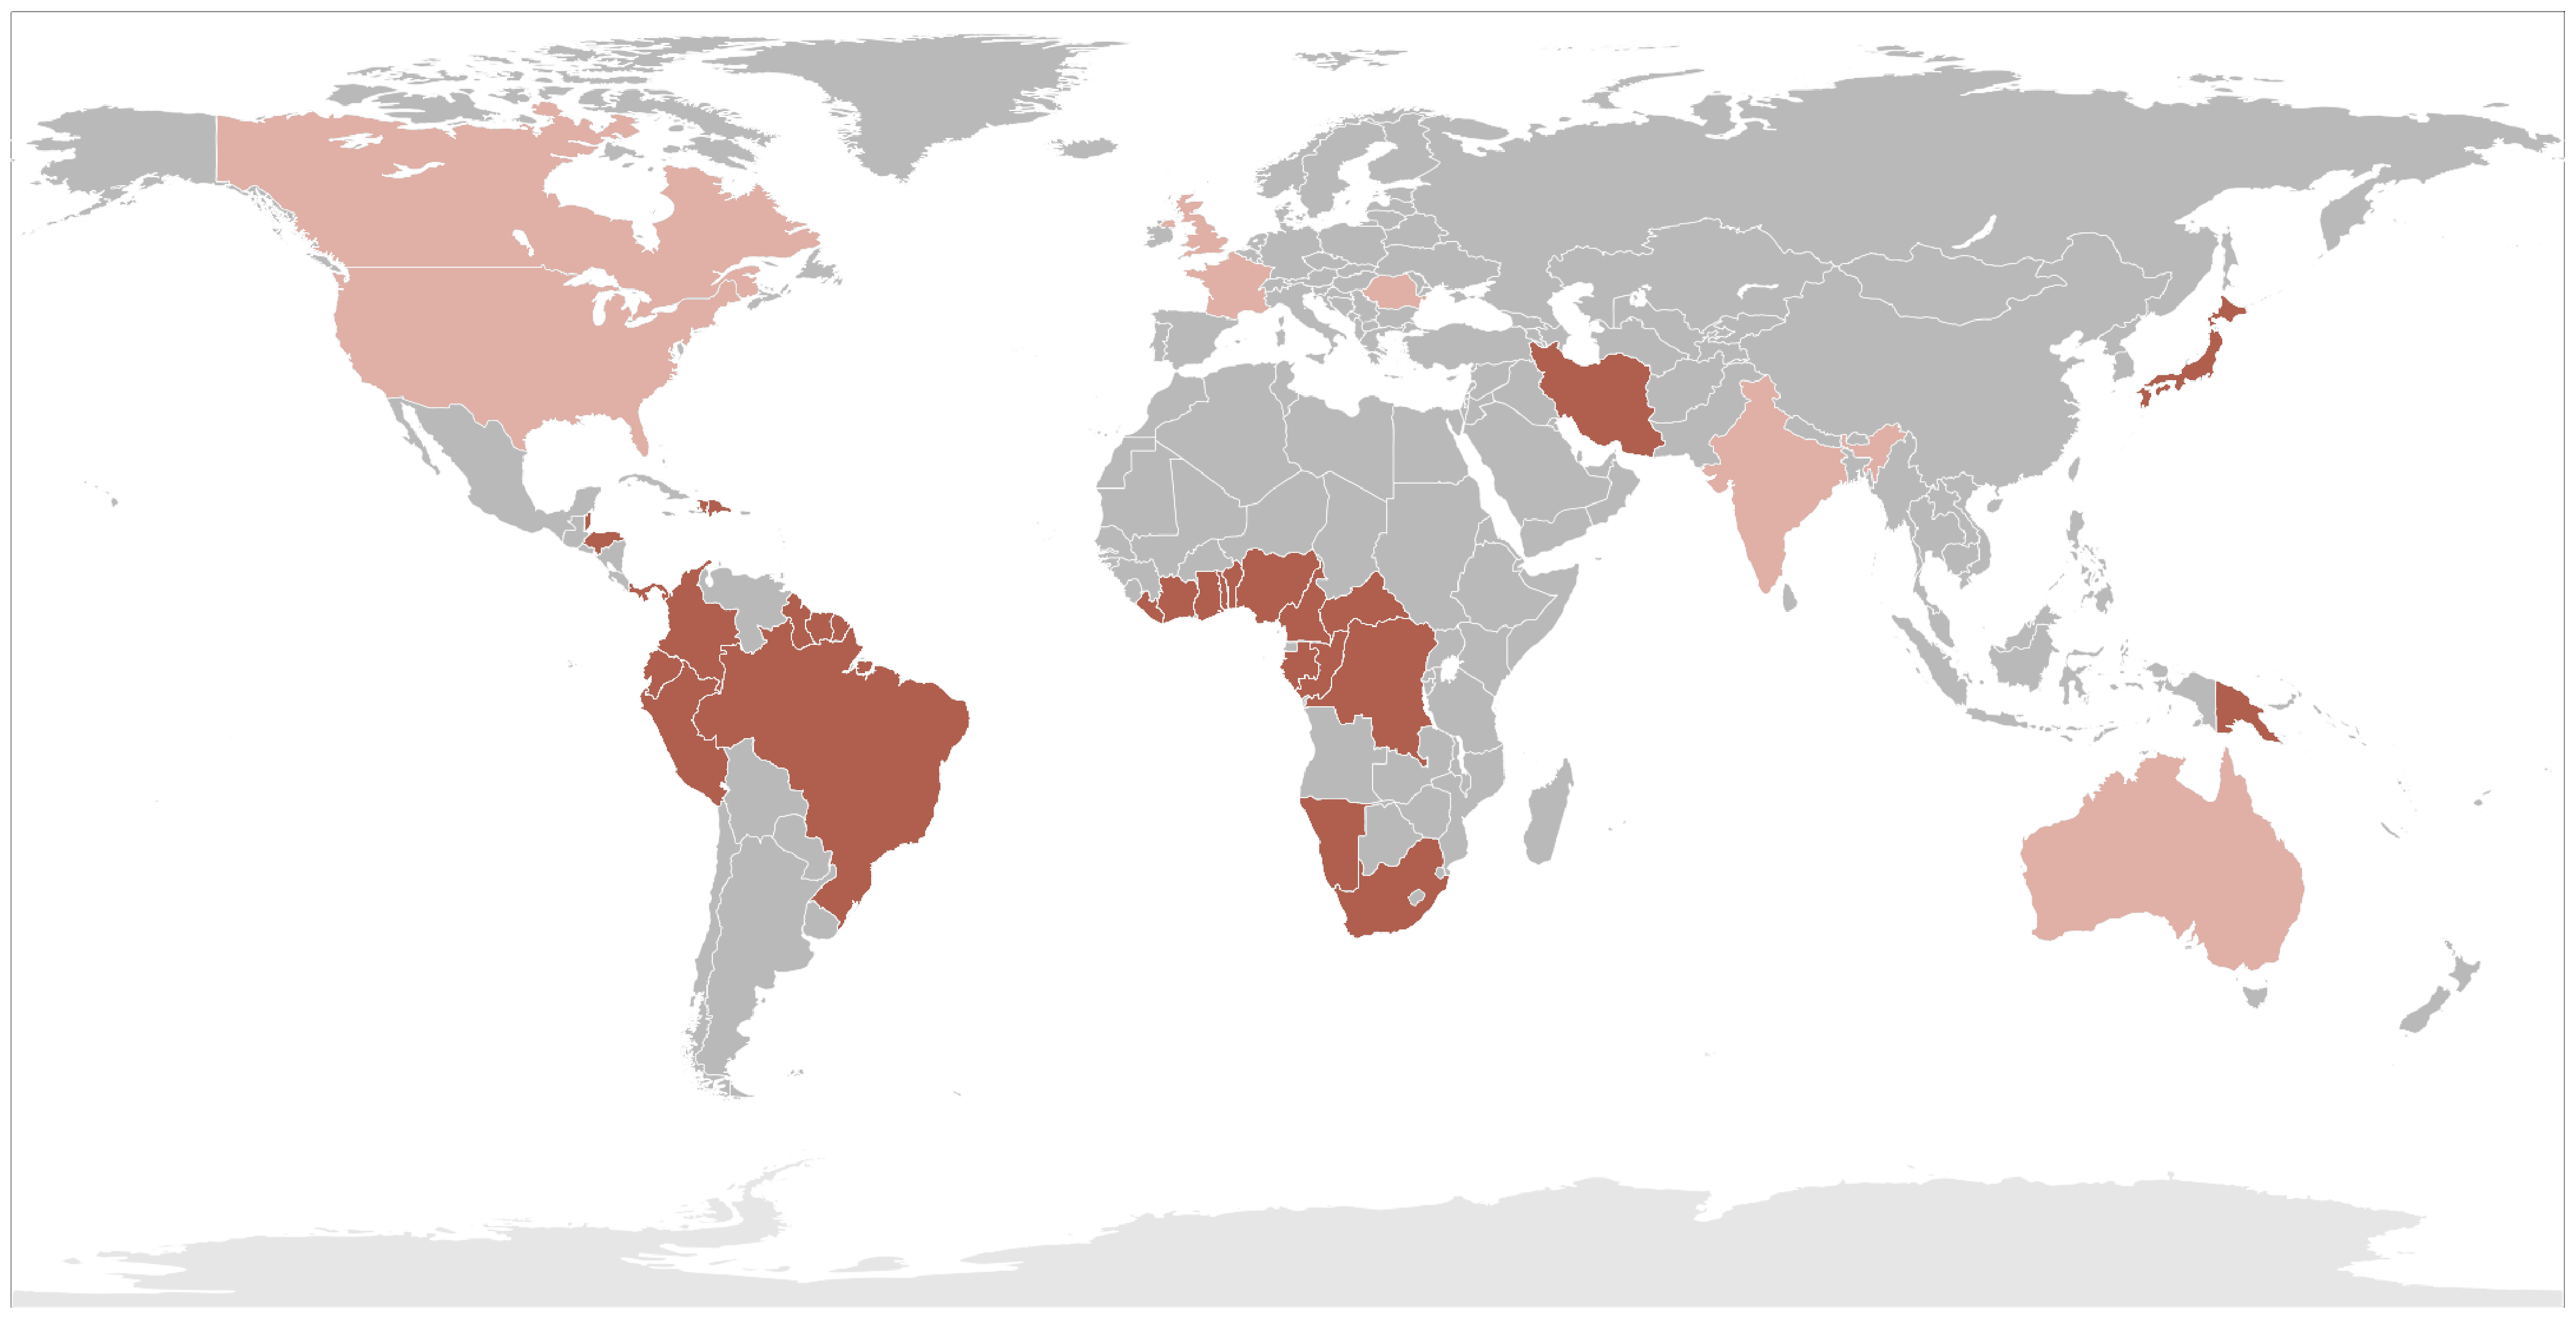
\includegraphics[width=14cm]{./Figures/chapter2/distribution}
\rule{35em}{0.5pt}
\caption[The global distribution of HTLV-I]{Countries with endemic HTLV-I, defined as prevalence between 1 and 5\% in some populations, are shown in dark red. Countries with reports of low prevalence (less than 1\% in some groups), due mainly to immigration from endemic areas, are shown in light red. It should be noted that HTLV-I endemic areas do not correspond exactly to the country boundaries shown in the map. For example in Brazil, Japan and Iran, HTLV-I is limited to residents of certain areas of each country. Data is from \citep{Proietti2005}.}
\label{chapter2/figure1}
\end{figure}

The virus is endemic to a number of geographically distinct regions across the world (\fref{chapter2/figure1}). In the Caribbean, 3-4\% of the population are seropositive for HTLV-I, in Africa the virus is detectable along an increasing gradient from north to equatorial Africa and in Japan, several regions have high incidences of seropositive individuals \citep{Edlich2000}. It can also be found in northern Iran, southern India and the aboriginal peoples of northern Australia. Other populations include immigrants from these endemic areas, as well as sporadic cases of HTLV-I among white Europeans with no identifiable risk factors. Overall, it is estimated to infect between 10 and 20 million people worldwide \citep{The1993}. It is a chronic infection which remains asymptomatic in the majority of cases. There is a maximum seroprevalance of 35\% in Okinawa, Japan \citep{Hinuma1982}.

The principal modes of transmission are transfer of infected CD4$^+$ lymphocytes from mother to child in breast milk, sexual transmission (especially from infected men to women via semen) and via inoculation/transfusion of infected blood. Cell-free blood products have a negligible risk because of the paucity of free virus particles present in plasma. Infection in endemic regions occurs mainly through breast-feeding, via the transfer of infected lymphocytes in the milk \citep{Hino1985}. However, infection can occur during the peri-natal period \citep{Hino1987} and transplacental transmission has been documented but is not thought to be common \citep{Komuro1983}. Male to female transmission is roughly 4 times higher than the converse \citep{Stuver1993} and the risk of infection is increased in the presence of genital ulceration, high proviral loads and high antibody titres \citep{Murphy1989, Kaplan1996}. The probability of seroconversion following transfusion of infected blood products is 50-60\% with a median time to conversion of 51 days \citep{Okochi1984, Manns1992}. Screening transfusion blood for HTLV-I is now routine in Brazil, Japan, the UK and the USA. There is an increasing prevalence of HTLV-I among intravanous drug users in both Europe and the USA \citep{The1993}.

\section{HTLV-I Associated Diseases}

Most HTLV-I-infected people remain healthy, but between 1-2\% will develop HAM/TSP, another 2-3\% develop ATL and a small number develop other less well defined inflammatory disorders. The factors deciding these outcomes are not fully understood but they are two distinct pathologies and the pathogenesis of the two appear to be very different. It has been thought that the occurrence of the two syndromes in the same person is not seen any more frequently than would be expected by chance. However, a high frequency of co-presentation of HAM/TSP and ATL has recently been reported in Bahia, Brazil \citep{Willems2009}.

\subsection{HTLV-I Associated Myelopathy/\\Tropical Spastic Paraparesis (HAM/TSP)}\label{chapter2/HAM/TSP}

The first descriptions of a myelopathy of unknown origin in tropical areas go back to the 19\superscript{th} century \citep{Strachan1888}. The association with HTLV-I was recognized independently in the Caribbean (as TSP) and in Japan (as HAM) in 1985-1986 \citep{Gessain1985, Osame1986}. The lifetime risk for developing HAM/TSP is between 2-7\%, except for Japan where it is estimated to be 0.25\% \citep{Kaplan1990, Taylor2000}.

\subsubsection{Pathology}\label{chapter2/path}

The main pathological feature of HAM/TSP is a chronic inflammation of the white and grey matter of the spinal cord. Mononuclear cells, mainly T cells, cause 
% perivascular cuffing - accumulation of lymphocytes / parenchyma
perivascular cuffing and infiltrate the parenchyma \citep{Verdonck2007}. The damage is concentrated in the white matter of the lower thoracic spinal cord, which causes the spastic paraparesis in the lower limbs \citep{Aye2000}. There is a possibility that the lesions in the central nervous system could be the consequence of a genuine anti-HTLV-I reaction. This is based on the observations that HAM/TSP patients have a higher proviral load, a higher production of proinflammatory cytokines in response to viral peptides (such as IFN-$\gamma$ and TNF$\alpha$) and a higher frequency of HTLV-I specific CD8$^+$ T-cells compared to asymptomatic carriers \citep{Olindo2005, Sakai2001, Goon2003, Montanheiro2005}. Polymorphism in the TNF$\alpha$ promoter and the chemokine gene SDF-1$\alpha$ have also been shown to influence the risk of HAM/TSP \citep{Vine2002}. Other evidence of an immunopathological reaction in the central nervous system is the observation of infected T-cells within the spinal cord lesions and the accumulation of Tax-specific CD8$^+$ T-cells in the cerebrospinal fluid \citep{Kubota2002, Muraro2003}. There is also a possibility that cross-reactivity between HTLV-I antigens and tissue antigens could be involved in the pathogenesis. This is based on a contentious finding that patients with HAM/TSP appear to develop antibodies to human neurons but not to systemic organs \citep{Levin2002}. Additionally, auto-antibodies against other nuclear and perinuclear human brain proteins cross-reacting with different HTLV-I epitopes have been found in the serum of HAM/TSP patients \citep{Garcia-Vallejo2005}. However, since inflammatory T-cells, rather than antibodies, seem to cause the tissue damage, autoreactivity at the level of the T-cell receptor may be more likely.

\subsubsection{Presentation}

The commonest presenting features in descending order are gait disturbance ($\sim2/3$ cases), urinary dysfunction ($>1/3$ cases), then numbness of the lower legs, constipation, lumbar back pain and hand tremors. The lower limbs are usually affected to a much greater degree than the upper limbs. The spasticity and associated upper motor signs can be very severe. Low back pain or ache is very common and affects most at some time during the course of the disease. The spectrum of disease progression is very variable, ranging from minimal gait disturbance maintained over the patient�s lifetime
to severe, very rapid progression and even death (rare). In one study cohort from Columbia, after a mean period of 14.4 years (range of 1 - 30 years), 34\% could walk unaided, 40\% required a walking aid, and 26\% required a wheelchair (otherwise bed-bound) \citep{Roman1988}.

\subsubsection{Treatment}

Therapies targeting the immune response have been considered for the treatment of HAM/TSP. Corticosteroids have been shown to be of some benefit \citep{Nakagawa1996} and interferon-$\beta$1a reduced HTLV-I mRNA load. However, the proviral load remained unchanged and there was only a slight improvement in motor function \citep{Osame1990} The combination of two nucleoside analogues (zidovudine and lamivudine) has been evaluated in a randomised, double-blind, placebo-controlled study including 16 HAM/TSP patients. After up to 12 months of follow-up, there were no significant changes in proviral load and no clinical improvement was observed \citep{Taylor2006}. Long term treatment studies have been formulated with valproic acid (VPA). VPA is a lysine deacetylase inhibitor and is postulated to work by activating viral gene expression and exposing virus-infected cells to the immune system, thus reducing proviral load. It has been shown to be safe but does not seem to alleviate the conditions of HAM/TSP \citep{Willems2009}. Additional strategies that have been proposed include minocycline (an antibiotic that inhibits monocyte/macrophage activation), humanized mik$\beta$1 (a monoclonal antibody against CD122, the $\beta$ subunit shared by IL2 and IL15) and the immunosuppressant cisclosporin \citep{Willems2009}.

\subsection{Adult T-cell Leukaemia/Lymphoma (ATL)}

ATL was first described in the 1970s when the observation of haematological malignancies did not fit previous pattern descriptions \citep{Yoshida2001}. It is a malignancy of CD4$^+$ post-thymic T-cells in which the HTLV-I provirus is integrated.

\subsubsection{Pathology}

The regulatory protein Tax induces abnormal growth of infected T-cells through several pathways \citep{Yoshida2001}. Tax promotes the transcription of its own proviral genome, but it also promotes transcription of cellular genes, including cytokine (e.g.~interleukin-2), cytokine receptor (interleukin-2Ra), and anti-apoptotic genes. By binding to other protein complexes, Tax represses the transcription of genes that are important in negative control of the cell cycle, in activation of apoptosis, and in DNA repair. Tax also binds and inhibits proteins directly involved in tumour suppression and DNA repair. Finally, Tax causes cells to bypass normal cell-cycle checkpoints \citep{Yoshida2001}. The net effect of all these activities of Tax is that T cells are rushed into and through the mitotic phase without checking for chromosomal abnormalities. Genetic damage that would normally be repaired accumulates and apoptotic cell death does not occur even in cells with severely damaged DNA. In these circumstances, T cells can accumulate DNA mutations, resulting in transformation and monoclonal outgrowth of a truly malignant cell. In addition to these genetic changes, epigenetic changes such as DNA methylation may have an important role in leukaemogenesis \citep{Taylor2005}.

\subsubsection{Presentation}

There are several types of HTLV-I induced ATL: acute, lymphotamous, chronic and smouldering \citep{Shimoyama1991}. Amost all patients with ATL present with lymphadenopathy (enlargement of the lymph nodes) and/or splenomegaly (enlargement of the spleen). ATL can also affect the lungs, gastrointestinal tract, and central nervous system; involvement of other organs is uncommon \citep{Shimoyama1991}. Hypercalcaemia is an important complication: it occurs in up to 70\% of patients and is often accompanied by lytic bone lesions. ATL patients are immunosuppressed and opportunistic infections, such as \emph{Pneumocystis jirovecii} pneumonia, cryptococcus meningitis, and disseminated herpes zoster are, therefore, frequent \citep{Roudier1997}. Liver dysfunction is another complication. The diagnosis of ATL is usually based on morphological analysis. Flower cells (i.e.~pleomorphic, atypical lymphoid cells with basophilic cytoplasm and convoluted nuclei) are indicators of acute or lymphoma-type ATL. This must be confirmed by clonal integration of HTLV-I provirus in the host genome.

\subsubsection{Treatment}

Acute ATL is very aggressive and highly refractory to treatment. Strategies that show an improvement over conventional chemotherapy in the treatment of ATL include Interferon-$\alpha$ with zidovudine, intensive chemotherapy and allogenic haematopoietic stem cell transplantation \citep{Taylor2005}. In fact, it is essential not to provide general chemotherapy (CHOP) to first line presenting ATL patients because this treatment selects for a tumor clone with mutated p53 \citep{Tsukasaki2009}. Nevertheless, the median survival of patients with acute, lymphomatous, and progressing chronic ATL remains low: less than 1 year in most reports \citep{Taylor2005}. Further improvements could include bortezomib (a proteasome inhibitor), anti-CD52 antibody, proapoptotic agents and consolidation with arsenic and IFN$\alpha$ \citep{Willems2009}. 

\subsection{Other Conditions Associated with HTLV-I}

HTLV-I has been associated with other inflammatory syndromes. In a Japanese cross-sectional study and a US cohort study, the prevalence and the incidence of arthritis were found to be higher among HTLV-I-infected patients than among uninfected individuals \citep{Eguchi1996,Murphy2004}. Tax transgenic mice have also developed an arthritis that is pathologically similar to human rheumatoid arthritis \citep{Iwakura1991,Yakova2005}.Tax has been shown to stimulate the proliferation of synovial cells in vitro \citep{Aono1998}. Hence, Tax, released by HTLV-I-infected cells in vivo, could have a part in the pathogenesis of arthropathy.

Reports from Japan have shown that HTLV-I infection is more frequent in patients with uveitis of unknown origin than in the general population \citep{Mochizuki1992}.The prognosis of HTLV-I-associated uveitis is good: spontaneously, the disease resolves within weeks and recovery is even faster with topical or systemic corticosteroid treatment. However, more than 90\% of cases recur within 3 years; the mean interval between episodes is 16 months \citep{Nakao1999}.

\emph{Strongyloides stercoralis} is an intestinal nematode of tropical regions that can replicate within the human host, an unusual characteristic among helminths. HTLV-I infection is associated with increased susceptibility to \emph{S. stercoralis} infection and a weak Th2 response is characteristic of this co-infection. As a result, the rate of parasite killing decreases and the rate of autoinfection increases \citep{Carvalho2004}. In rare cases this can result in the fatal Strongyloides hyperinfection syndrome \citep{Marcos2008}.

\section{Pathogenesis of HTLV-I}\label{chapter2/pathogenesis}

\subsection{Background}

1-2\% of HTLV-I infected subjects develop HAM/TSP and 2-3\% develop ATL. The factors deciding these outcomes of infection are not understood.

\subsection{Genotype}

Compared with HIV, HTLV-I is relatively stable in terms of sequence variation and mutation rate. However, the effect of mutation on the pathology of HTLV-I is still considered a possible variant in disease outcome. As a result, HTLV-I has been the subject of a range of studies looking at mutation and variability and how this affects the immune response to the virus. The majority of these studies have focused on \gene{tax}, as it is a dominant target for the CD8$^+$ immune response \citep{Goon2004}. Furukawa \emph{et al.} \citep{Furukawa2000} found phylogenetic subgroups in the \gene{tax} gene, one of which was associated with an increased risk of HAM/TSP. This result followed on from a number of studies from Niewiesk \emph{et al.} that focused on Tax expression. 

Initially, Niewiesk \emph{et al.} found that general \gene{tax} sequence variability (and not the presence of a specific sequence) was significantly greater in healthy seropositive individuals, compared to those presenting HAM/TSP \citep{Niewiesk1994}. This was followed by results showing that amino acid substitutions occurring in known Tax epitopes abolished T cell recognition. These substitutions were also associated with the allele \gene{HLA-A2} and reduced the transactivation function of Tax \citep{Niewiesk1995}. However, it was then found that this distinction in the mutation rate of \gene{tax} between healthy individuals and those with HAM/TSP could only be seen with proviral \gene{tax} sequences, but not with cDNA \citep{Niewiesk1996}. Kubota \emph{et al.} looked at synonymous and nonsymonymous \gene{tax} mutations in \gene{HLA-A*02} HAM/TSP patients to detect positive selection pressures \cite{Kubota2007}. They found pressures on three of six CTL epitopes tested, suggesting that CTLs eliminate infected cells \emph{in vivo} and also demonstrating that variant viruses do not accumulate. Once again, this reinforced the observation that Tax is functionally constrained in terms of mutations. Although research on Tax has predominated, some work on other proteins has also been completed. Furukawa \emph{et al.} showed that sequence variation in p12 may be associated with different outcomes to HTLV-I infection \citep{furukawa2004}. The Rex protein was also examined and shown to have strong functional constraints on amino acid variation \citep{Smith1997}. 

\subsection{The CTL Response to HTLV-I}\label{chapter2/CTLResponse}

The CTL response plays a central role in deciding the outcome of viral infections. It has been shown through evidence accrued from host and viral genetics, gene expression microarrays and assays of T-cell phenotype and function that individual differences in the efficiency of the virus-specific CTL response strongly determine the outcome of infection with the human retroviruses HTLV-I and HIV-I. From this evidence, it is now believed that differences in the anti-viral CTL efficiency at the single-cell level are responsible for variation in the efficacy of the host response to viruses.

Perhaps the strongest evidence that the CTL response is instrumental in controlling HTLV-I infection comes from the association of certain MHC class I alleles and protection from disease. Studies of HTLV-I genotype show significant associations between class I alleles (HLA-A*02 and HLA-Cw*08) and a reduced proviral load, which would implicate the CTL response as a positive factor \cite{Jeffery1999, Jeffery2000}. The hypothesis that extends from these results is that HLA-A*02 and HLA-Cw*08 restricted CTLs are more efficient at killing HTLV-I infected cells. Conversely, HLA-B*54 restricted CTLs, which have been associated with increased proviral load~\cite{Jeffery1999}, would produce a less efficient response.

The frequency of virus-specific CTL has been used to demonstrate the efficiency of the CTL response in HTLV-I infection with different conclusions. There is evidence that the frequency of HTLV-I-specific CD8$^+$ T cells differs little among patients with widely differing proviral load \citep{Parker1994}. However it has also been reported that HTLV-I-specific CTL frequency was positively correlated with proviral load \citep{Kubota2000}. These contradictory results demonstrate the difficulty of using CTL frequency as a marker of viral control in a chronic infection: since CTL proliferate in response to antigen, the frequency of CTL is both a cause and an effect of the viral load. Hence, a more effective metric of CTL efficiency is a measurement variable that accurately reflects an efficient CTL response.

CD8$^+$ cell attributes such as T-cell receptor avidity, specificity, and cell maturation state may all affect the ability of CD8$^+$ cells to control a viral infection. However, Asquith \emph{et al.} devised a combined measure by measuring the rate at which naturally, endogenously infected cells were cleared by autologous CD8$^+$ cells \emph{ex vivo} \citep{Asquith2005a}. This antiviral efficacy can be summarised by \eref{chapter2/equation1}: 

\begin{equation}
\frac{dy}{dt} = c - \epsilon y z
\label{chapter2/equation1}
\end{equation}

where $y$ is the proportion of CD4$^+$ cells expressing Tax, $c$ is the rate of increase of Tax expression, $\epsilon$ is the CD8$^+$ cell-mediated antiviral efficacy and $z$ the proportion of lymphocytes that are CD8$^+$. This approach yielded the conclusions that there was a significant negative correlation between the per-CD8$^+$ cell lysis rate and the proviral load, in both ACs and HAM/TSP patients. Also, the percentage of between-individual variation observed in the proviral load that was attributable to variation in the lysis rate parameter was about 35\% \citep{Asquith2005a}. From this data, it was predicted that CTL lysis would reduce the life expectancy of a virus-expressing target cell from the normal 30 days (for a memory phenotype, CD4$^+$CD45RO$^+$ T cell) to between 1 and 10 days. This was confirmed by measurement of infected T-cell turnover rate \emph{in vivo} by the metabolic labeling of lymphocytes with deuterated glucose \citep{Asquith2007a}.

The functional avidity is the concentration of antigen that is required to elicit the half-maximal effector response (usually
cytokine) in CD8$^+$ T cells. It has been widely used as a marker of the responsiveness or sensitivity of CTL to cognate antigen. In HTLV-1 infection, Kattan \emph{et al.} \citep{Kattan2009} found that avidity was correlated with per-CD8$^+$ lytic activity, measured by the CD8-dependent elimination of Tax$^+$ cells. The use of CD107a staining of CD8$^+$ T cells as a marker of the recent degranulation activity of HTLV-I-specific CD8$^+$ T cells has also shown differences between HAM/TSP patients and ACs; HAM/TSP patients produced a greater frequency of specific CD8$^+$ T cells but less CD107a staining per cell than ACs \citep{Sabouri2008}.

Taken together, this data emphasizes the role of CTL in HTLV-I control. It is clear that the HTLV-I-specific CTL response plays a critical role in limiting the replication of HTLV-I, the proviral load, and the risk of HAM/TSP. However, any understanding of the role of the CTL response in HTLV-I infection must acknowledge the seemingly detrimental effects of this response to the host (\sref{chapter2/path}).  

\subsection{The Antibody Response to HTLV-I}

Anti-Gag antibodies are the first specific antibodies to appear in response to the infection in the first 2-3 months. Anti-Env antibodies can then be detected, along with anti-Tax antibodies in 50\% of infected people \citep{Manns1992, Mueller1997}. Anti-HTLV-I antibody titres correlate with the provirus load and can be extremely high. It is currently unknown whether these antibodies play a part in protection against HTLV-I infection, against disease or are involved in the pathogenesis of disease.

Levin \emph{et al.} \citep{Levin2002} have described a putative autoantigen; neuronal heterogeneous nuclear ribonuclear protein-A1 (hn-RNP-A1), which stained brightly with IgG from HAM/TSP patients and not ACs. These IgG were also found to cross-react with HTLV-I Tax protein and stained human Betz cells specifically. Furthermore, the authors infused these antibodies onto rat brains and showed inhibition of neuronal activity. Thus, they concluded that HAM/TSP is an autoimmune disease, with molecular mimicry between an HTLV-I antigen and a self one causing the generation of cross-reacting antibodies and subsequent neurological disease.

\subsection{Other Immune Responses to HTLV-I}\label{chapter2/OtherImmune}

T\subscript{reg} cells are defined as CD4$^+$ T cells that inhibit immunopathology or autoimmune disease \emph{in vivo} \citep{O'Garra2004a}. The subset that has been studied with respect to HTLV-I is characterized by the expression of the glycoproteins CD4 and CD25, as well as the transcription factor Foxp3 \citep{O'Garra2004a}. Their role in HTLV-I infection is not yet fully understood but different T\subscript{reg} responses have been associated with both ATL and HAM/TSP. In terms of HAM/TSP, a number of studies have found that in T\subscript{reg} cells infected with the virus, both mRNA and protein expression of Foxp3 were lower in HAM/TSP patients compared to healthy carriers \citep{Yamano2005, Oh2006}. This has lead to the hypothesis that defects in T\subscript{reg} expression as a result of viral infection could cause the chronic inflammatory response characteristic of HAM/TSP \citep{Fujinami2005}. However, this conclusion remains very uncertain because HTLV-I strongly induces expression of CD25 (a marker of T\subscript{reg} cells) and it is therefore inappropriate to use CD25$^+$ as part of the definition of T\subscript{reg} cells in HTLV-I infection (C. Bangham, pers. comm.).

In terms of ATL, several studies have shown the expression of Foxp3 in the tumour cells of a subset of patients with ATL \citep{Yano2007}. Yano \emph{et al.} demonstrated these cells continue to act as regulatory T cells and that their proliferation may be the cause of the severely immunocompromised state of ATL patients \citep{Yano2007}. 

The natural killer (NK) cell response to HTLV-I has received less attention, partly because of the difficulty in identifying NK cells in terms of their surface markers and the existence of NK cell subsets \citep{Bangham2005}. However, an association has been found between the low frequency of CD3$^+$ NK cells and patients with HAM/TSP \citep{Saito2003, Yu1991, Fujihara1991}, suggesting a role for this subset of NK cells in disease progression. Other data on lymphocyte gene expression also indicated that high levels of expression of certain genes involved in NK cell-mediated lysis were associated with low proviral load of HTLV-I \citep{Vine2004}. This would suggest that, along with CD8$^+$ CTLs, NK cells are part of the cytolytic lymphocytes that reduce HTLV-I proviral load.

The CD4$^+$ (helper) T cell response has been difficult to study as Tax in infected CD4$^+$ T cells produces effects (IFN$\gamma$ production, T-cell proliferation), which are also the basis of CD4$^+$ T cell response assays \citep{Bangham2005}. Hence, the presence of HTLV-I would interfere with any analysis on CD4$^+$ T cell response. However, using a modified assay \citep{Goon2002}, it has been demonstrated that the response is predominantly IFN$\gamma$-producing cells. Also the frequency of IFN$\gamma$ producing CD4$^+$ T cells was between 10 and 25 times greater in HAM/TSP patients compared with asymptomatic carriers \citep{Goon2003}. From this information, it is likely that these cells contribute to the chronic inflammatory response seen in HAM/TSP. 

\section{Epitope Prediction}\label{Introduction/Prediction}

As mentioned in \cref{Chapter1}, \sref{chapter1/EpPred} it was necessary to use epitope prediction software to predict the HTLV-I peptides that bind to different MHC class I alleles. This type of prediction software uses a range of mathematical methods to recognize the small number of pathogenic peptides that can bind to MHC class I and hence elicit a CTL immune response.

Of the large number of peptides that can be derived from a pathogen only a small minority, approximately 1 in 2,000, elicits a CTL response \citep{Yewdell1999}. This limitation in the number of peptides that are immunogenic is conferred by three main constraints: the requirement for peptide cleavage and transport, the requirement for MHC-peptide binding and the requirement for CTL recognition. By far the most stringent of these is the requirement for MHC-peptide binding, because only 1 in 200 peptides binds a specific MHC molecule with sufficient affinity to elicit an immune response \citep{Yewdell1999}. Further selection is largely due to the limitations of peptide processing and transport. In these processes, individual peptides are produced from the precursor polypeptides by proteasomal cleavage of the polypeptide, which can be followed by N-terminal trimming by other peptidases. This is followed by the transport of the peptides from the cytosol to the endoplasmic reticulum, mediated by the TAP complex. Further N-terminal trimming may occur before the peptide binds to the MHC molecule. The requirements of processing and transport eliminate approximately 80\% of potential epitopes \citep{Yewdell1999}. Finally, T cell specificity, i.e. the requirement for T cell receptor binding of the MHC-peptide complex, further halves the number of presented peptides that elicit a response. The probability of each of these steps is determined by the polypeptide sequence, amongst other factors \citep{larsen2005}.

The identification of T cell epitopes is of vital importance in the design of vaccines and understanding of the immune system \citep{bui2006, sette2005, sette2007, sathiamurthy2005}. However, given the scarcity of epitopes, experimentally screening all possible peptides for each MHC allele (e.g. by IFN$\gamma$ ELISpot) is time consuming, expensive and inefficient. One way to improve the efficiency of the identification process is to first use theoretical algorithms to predict which peptides are more likely to be epitopes and then experimentally screen this much smaller, selected list of peptides. This method is widely used \citep{snyder2004, tscharke2005, drexler2003, oseroff2005, pasquetto2005} and has been applied in a number of studies to identify potential vaccines \citep{wang2007a, thorn2007}. The use of theoretical methods to "pre-screen" peptides is of particular importance in the case of emerging infections such as avian influenza \citep{wang2007} where rapid vaccine development would be vital. This approach also underpins a large bio-preparedness initiative coordinated by the Large-Scale Antibody and T Cell Epitope Discovery Program \citep{sette2005}, which intends to foster development of immune-based therapeutics for emerging and reemerging pathogens including potential bioterrorism agents. More generally, epitope prediction algorithms are being increasingly used to understand the CTL response. For example, in the case of HIV-I infection, algorithms have been used to confirm which epitope mutations are likely to confer escape from a CTL response \citep{brumme2007} and to understand why some MHC class I alleles are associated with slow rates of disease progression \citep{borghans2007}.

A range of computational algorithms have been developed to predict CTL epitopes in pathogen protein sequences. Since the most selective requirement for a peptide to be immunogenic is the ability of the peptide to bind to the MHC molecule, most prediction methods focus on this stage of the pathway. As a general rule, information gained from experimental binding assays is used to train the algorithm until it is efficient at predicting novel MHC-peptide complexes. The algorithms that are used vary in complexity and accuracy. Some can be trained to recognize peptide motifs that are required for binding to a particular MHC molecule \citep{rammensee1999}, others use a weight-matrix method to identify amino acids that occur at a higher-than-expected frequency at specific epitope positions \citep{nielsen2004, bui2005, peters2005a}. However, the most accurate methods available use logistic regression \citep{heckerman2007} and, more generally, artificial neural networks \citep{larsen2005, tenzer2005}.

Artificial neural networks (ANNs) take into account, in addition to the identity of each amino acid residue, the interactions between adjacent amino acids in a potential epitope. In summary, an ANN for a particular MHC molecule is trained to recognize associated inputs (a peptide sequence) and outputs (the binding affinity for that sequence with the MHC molecule) \citep{buus2003}. Once an ANN is trained for a particular molecule, it can predict the binding affinity of novel peptide sequences.

NetCTL \citep{larsen2005} and NetMHC \citep{buus2003, nielsen2003, nielsen2004} are two of the most accurate prediction methods currently available \citep{peters2005}. NetMHC uses ANNs for a number of alleles to predict MHC molecule-peptide binding affinities. NetCTL, as well as using the same ANNs to predict MHC-peptide binding, also utilizes information about the proteasomal cleavage of the input peptide sequence, and its ability to bind to TAP. NetCTL or NetMHC will predict a score (either integrated or simply a binding affinity, respectively) for every overlapping nanomer peptide sequence in an input sequence to each MHC molecule for which the method has an ANN. Henceforth, we refer to the trained prediction algorithm for each MHC class I allele as an "allelic predictor".	% Introduction
% Chapter 3

\chapter{Identifying Alleles Associated with Disease Status and Proviral Load} 
\label{Chapter3}
\lhead{Chapter 3. \emph{Identifying Alleles Associated with Disease Status and Proviral Load}}

\section{Introduction}

Jeffery \emph{et al.} \citep{Jeffery1999, Jeffery2000} demonstrated the protective effects of the MHC class I alleles A*02 and Cw*08 in terms of disease status and a reduced proviral load in asymptomatic carriers of HTLV-I. It was also shown that B*5401 is associated with a greater risk of HAM/TSP and with a higher proviral load in HAM/TSP patients. Added to this, results showing that class I heterozygosity is associated with significantly lower proviral loads \citep{Jeffery2000} would suggest that the protective effect of the HLA haplotype extends to a range of alleles.

Using the same Kagoshima database as previous studies \citep{Jeffery1999, Jeffery2000}, our initial task was to reanalyze this data in an attempt to broadly classify the HLA class I alleles contained within the cohort into `detrimental', `beneficial' and `undefined' groups, according to their associations with disease risk and proviral load. This design would increase the power of the next stage of our study - understanding the functional basis of these associations though analysis of the HLA class I alleles' HTLV-I epitopes.

Hence, the aim of this chapter was to analyze the HLA class I repertoire of the Kagoshima cohort in terms of its association with proviral load and disease risk, using classical and novel nonparametric statistical methods.

\section{Methods}\label{chapter3/methods}

\subsection{The Kagoshima Dataset}\label{chapter3/kagoshima}

All HAM/TSP and AC subjects for this study were of Japanese ethnic origin, and resided in Kagoshima prefecture (1988 population: 1.7 million), southern Kyushu, Japan, where the seroprevalence of HTLV-I infection in adults is approximately 10\% \cite{Osame1986, Nakagawa1995}. The estimated prevalence of HAM/TSP in the HTLV-I positive population is less than 1\% \cite{Kaplan1990}. For the purposes of this study, 230 cases of HAM/TSP were compared with 202 randomly selected HTLV-I seropositive asymptomatic blood donors (asymptomatic carriers - ACs) from the Kagoshima Red Cross Blood Transfusion Service. The diagnosis of HAM/TSP was made according to World Health Organisation (WHO) criteria \cite{Osame1990}.

\subsection{Disease Risk}

The Yates $\chi^{2}$ test has been used to test the relationship between disease risk and the presence of an allele. The test takes as its input a matrix (table \ref{tables/chapter_4/table_1}) and examines the null hypothesis that the observed frequency of alleles in each population (HAM/TSP and asymptomatic carriers) is the same as the expected frequency. The Yates correction applied in each case is used to prevent overestimation of statistical significance for small amounts of data. 

\begin{table}[htbp]
\centering
\begin{tabular}{lll}
 & \textbf{A$^+$} & \textbf{A$^-$} \\
\hline
\textbf{D} & a & b \\
\textbf{H} & c & d \\
\hline
\end{tabular}
\caption[The input matrix for the $\chi^{2}$ test]{The input matrix for the $\chi^{2}$ test, where D = disease, H = health, A$^+$ = positive for protective allele and A$^-$ = negative for protective allele.}
\label{tables/chapter_4/table_1}
\end{table}

\subsection{Proviral Load}\label{chapter3/methodsLoad}

We used the Mann-Whitney $U$ test to examine the null hypothesis that the presence of a single allele had any effect on proviral load. This analysis was performed separately for HAM/TSP patients and asymptomatic carriers (ACs) as there is a very strong association between HAM/TSP and high proviral load. 

A novel ranking test was also formulated to examine the robustness of each allele's association with proviral load. For both groups (HAM/TSP and ACs), the following was performed: 

\begin{itemize}
	\item The individuals in each group were randomly assigned to two separate populations.
	\item For each of the two populations, the alleles were ranked in terms of the median proviral load associated with that allele (i.e.~the median proviral load of all individuals who possessed that specific allele). This random assignment was reiterated 1,000 times. 
	\item The result of this was 2,000 rank positions for each allele in terms of median proviral load. 
	\item The median rank and confidence intervals were then compared. 
\end{itemize}

\section{Results}

\subsection{Proviral Load}\label{chapter3/ResultsLoad}

\fref{chapter3/figureLoad} shows the results of the initial analysis of multiple Mann-Whitney $U$ tests for each allele. 

\fref{chapter3/figureRobust} shows the results of the robustness of rank measure in terms of proviral load. Any allele showing a narrow confidence interval is demonstrating a robust rank in the face of random sampling from the proviral load associated with it. For example, in the HAM/TSP results, we can be confident in the designation of HLA-A*03 as a 'good allele' in terms of proviral load, owing to its position on the x-axis and the narrowness of the confidence interval. From this data, alleles were designated as positive or negative according to the non-overlapping of their confidence intervals (\tref{chapter3/tableSummary}).

\subsection{Disease Risk}\label{chapter3/ResultsRisk}

\fref{chapter3/figureChi} shows the alleles ranked in terms of disease risk. These results show an obvious overlap with previous research (the significant results of A*02, B*54 and Cw*08) and the possibility of other candidate alleles (B*48).

\begin{table}[htp]
\begin{center}
\begin{sideways}
{
\scriptsize
\begin{tabular}{|c|c|c|c|c|c|c|c|c|c|c|}
\hline
Names & $P$ HAM/TSP & HAM/TSP Effect & $P$ AC & AC Effect & $P\ \chi^2$ & $\chi^2$ Effect & HAM/TSP Rank & AC Rank \bigstrut \\
\hline
A01 & 0.0000 & NA & 0.1786 & protective & 0.0000 & NA & & protective \bigstrut[t] \\
A02 & 0.3003 & protective & 0.0161 & protective & $< 0.0001$ & protective & & \\
A03 & 0.1464 & protective & 0.7909 & protective & 0.5261 & protective & protective & \\
A11 & 0.3999 & protective & 0.9211 & protective & 0.3635 & detrimental & & \\
A24 & 0.4787 & detrimental & 0.3681 & detrimental & 0.1474 & detrimental & & \\
A26 & 0.5197 & protective & 0.0437 & detrimental & 0.8559 & detrimental & & detrimental \\
A30 & 0.0568 & protective & 0.0000 & NA & 0.0000 & NA & protective & \\
A31 & 0.7096 & detrimental & 0.9037 & protective & 0.2681 & detrimental & & \\
A32 & 0.2803 & protective & 0.1786 & protective & 0.5365 & protective & protective & protective \\
A33 & 0.1514 & detrimental & 0.3850 & protective & 0.2995 & detrimental & detrimental & \\
B07 & 0.0230 & protective & 0.0963 & detrimental & 0.1035 & detrimental & & \\
B13 & 0.7524 & protective & 0.5186 & detrimental & 0.4508 & detrimental & & \\
B15 & 0.2597 & protective & 0.2601 & protective & 0.1281 & protective & & \\
B27 & 0.5412 & detrimental & 0.4263 & protective & 0.8839 & protective & detrimental & \\
B35 & 0.1039 & protective & 0.4310 & detrimental & 0.5841 & protective & & \\
B37 & 0.0000 & NA & 0.1786 & protective & 0.0000 & NA & & protective \\
B38 & 0.1893 & protective & 0.0000 & NA & 0.0000 & NA & protective & \\
B39 & 0.3045 & detrimental & 0.7824 & detrimental & 0.6011 & protective & & \\
B40 & 0.4786 & detrimental & 0.5709 & protective & 0.1104 & protective & & \\
B41 & 0.0000 & NA & 0.7562 & detrimental & 0.0000 & NA & & detrimental \\
B44 & 0.2169 & protective & 0.0733 & protective & 0.4486 & protective & & \\
B46 & 0.9813 & detrimental & 0.7261 & protective & 0.4279 & protective & & \\
B48 & 0.7705 & protective & 0.4001 & protective & 0.0263 & protective & & \\
B51 & 0.3067 & detrimental & 0.7686 & detrimental & 0.3218 & detrimental & & \\
B52 & 0.6364 & detrimental & 0.3742 & detrimental & 0.5040 & protective & & \\
B54 & 0.0034 & detrimental & 0.8505 & detrimental & 0.0008 & detrimental & detrimental & \\
B55 & 0.6298 & detrimental & 0.3022 & protective & 0.5622 & detrimental & & \\
B56 & 0.1452 & detrimental & 0.4664 & protective & 0.7439 & detrimental & detrimental & \\
B57 & 0.0000 & NA & 0.7432 & detrimental & 0.0000 & NA & & detrimental \\
B58 & 0.3457 & detrimental & 0.8068 & detrimental & 0.3748 & detrimental & & \\
B59 & 0.9265 & detrimental & 0.9980 & protective & 0.5947 & protective & & \\
B67 & 0.9677 & protective & 0.6816 & detrimental & 0.8012 & protective & & \\
C01 & 0.0716 & detrimental & 0.2828 & protective & 0.1416 & detrimental & detrimental & \\
C03 & 0.1176 & protective & 0.4690 & detrimental & 0.1659 & protective & & \\
C04 & 0.7755 & detrimental & 0.4697 & detrimental & 0.8566 & detrimental & & \\
C05 & 0.2803 & protective & 0.0438 & protective & 0.5261 & protective & protective & protective \\
C06 & 0.0161 & protective & 0.1786 & protective & 0.7092 & detrimental & protective & protective \\
C07 & 0.3218 & protective & 0.1859 & detrimental & 0.2001 & detrimental & & detrimental \\
C08 & 0.2647 & protective & 0.0466 & protective & 0.0029 & protective & & \\
C12 & 0.8432 & protective & 0.6302 & detrimental & 0.9447 & protective & & \\
C14 & 0.2828 & detrimental & 0.9638 & protective & 0.2323 & detrimental & & \\
C15 & 0.0170 & protective & 0.9644 & detrimental & 0.1904 & protective & protective & \bigstrut[b] \\
\hline 
\end{tabular}
}
\end{sideways}
\end{center}
\caption[The summary of allele association statistics]{The summary of allele association statistics. The first 4 columns give the $P$ values and the direction of effect for the Mann-Whitney $U$ tests of proviral load in both HAM/TSP patients and ACs for alleles in the Kagoshima cohort (\fref{chapter3/figureLoad}). For each allele, the proviral load of individuals with and without the allele was compared. The next 2 columns show the significance and direction of disease risk associated with the allele in question (\fref{chapter3/figureChi}). The last 2 columns show the significant results of the robustness of rank measure (\fref{chapter3/figureRobust}). For both HAM/TSP patients and ACs, alleles are described as `positive' if their upper confidence limit does not overlap with the lower confidence limit of the `detrimental' alleles (and conversely for the detrimental alleles).}
\label{chapter3/tableSummary}
\end{table}

\begin{figure}[htp]
\centering
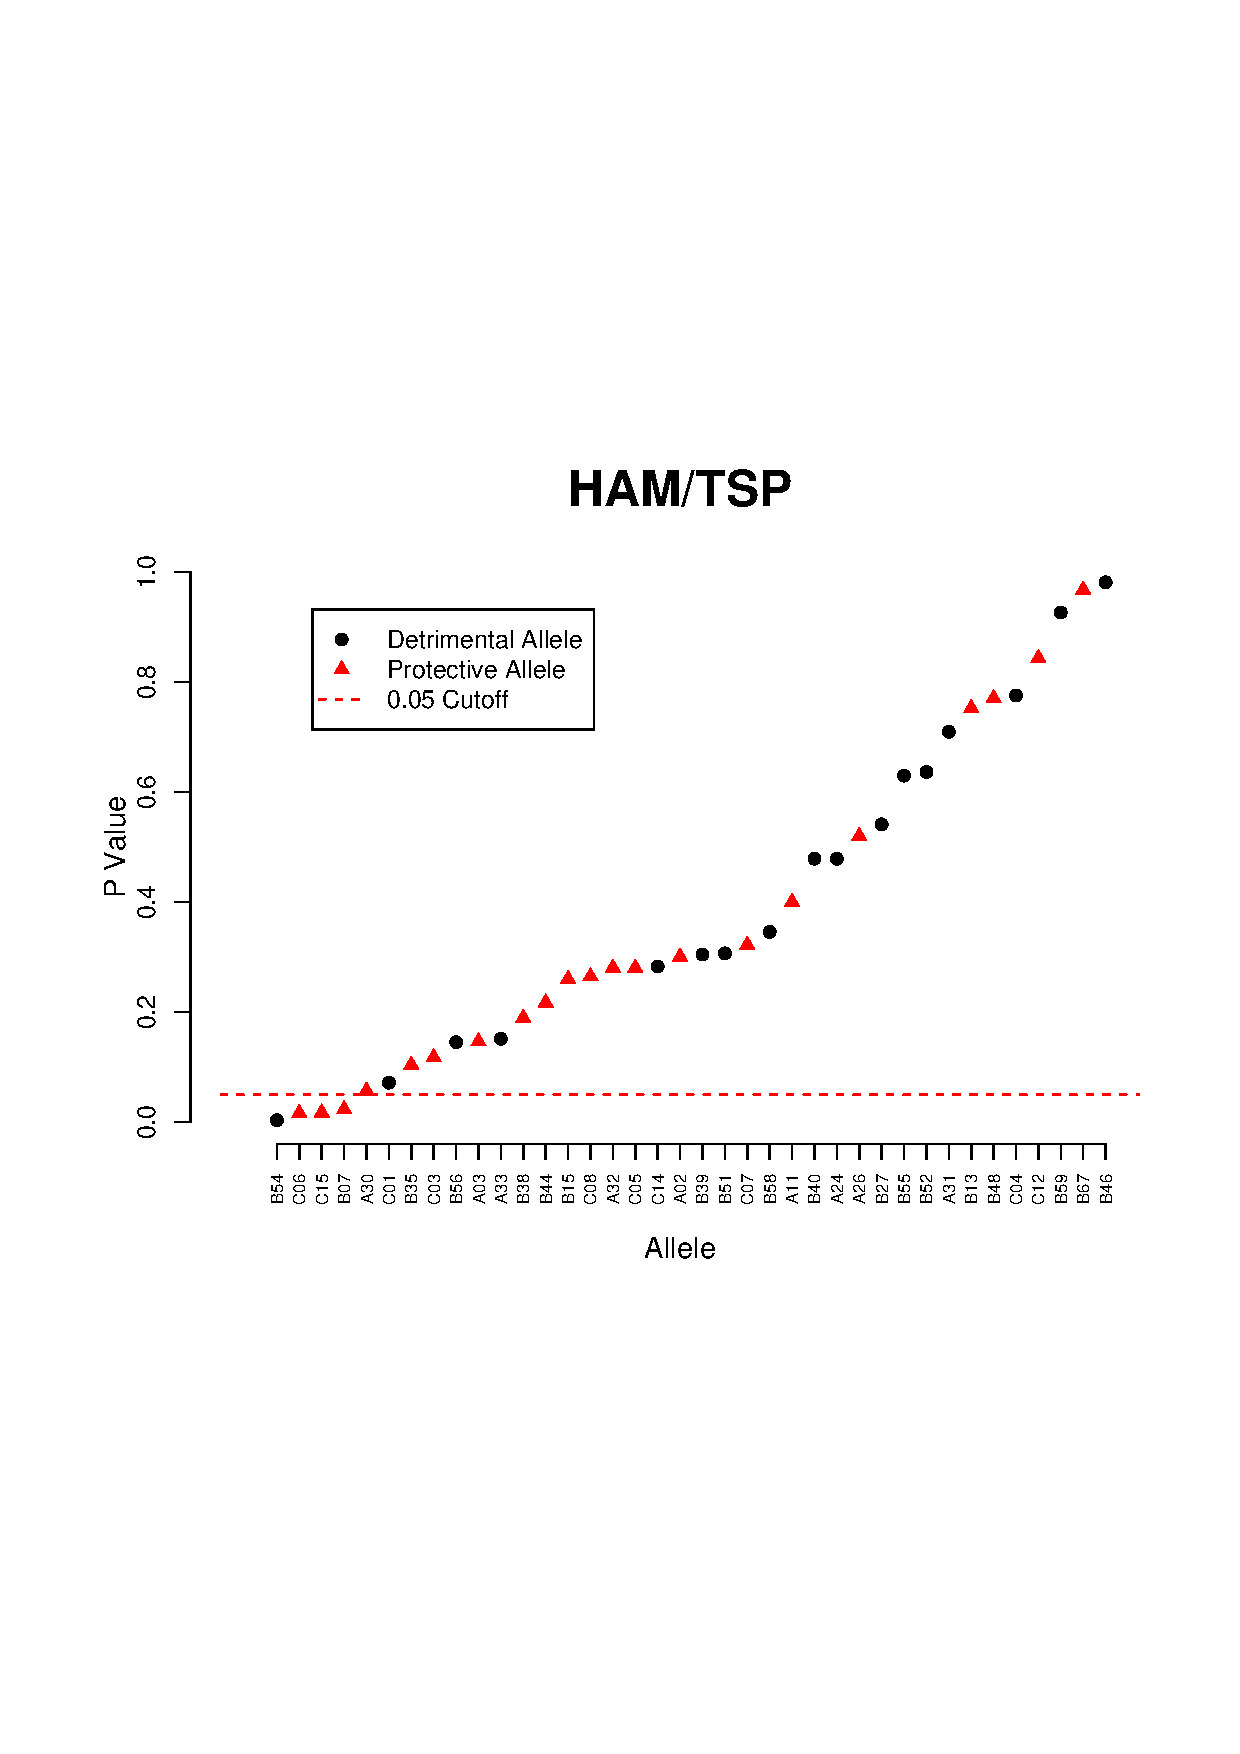
\includegraphics[width=14cm]{./Figures/chapter3/figureWilcoxHam} \\
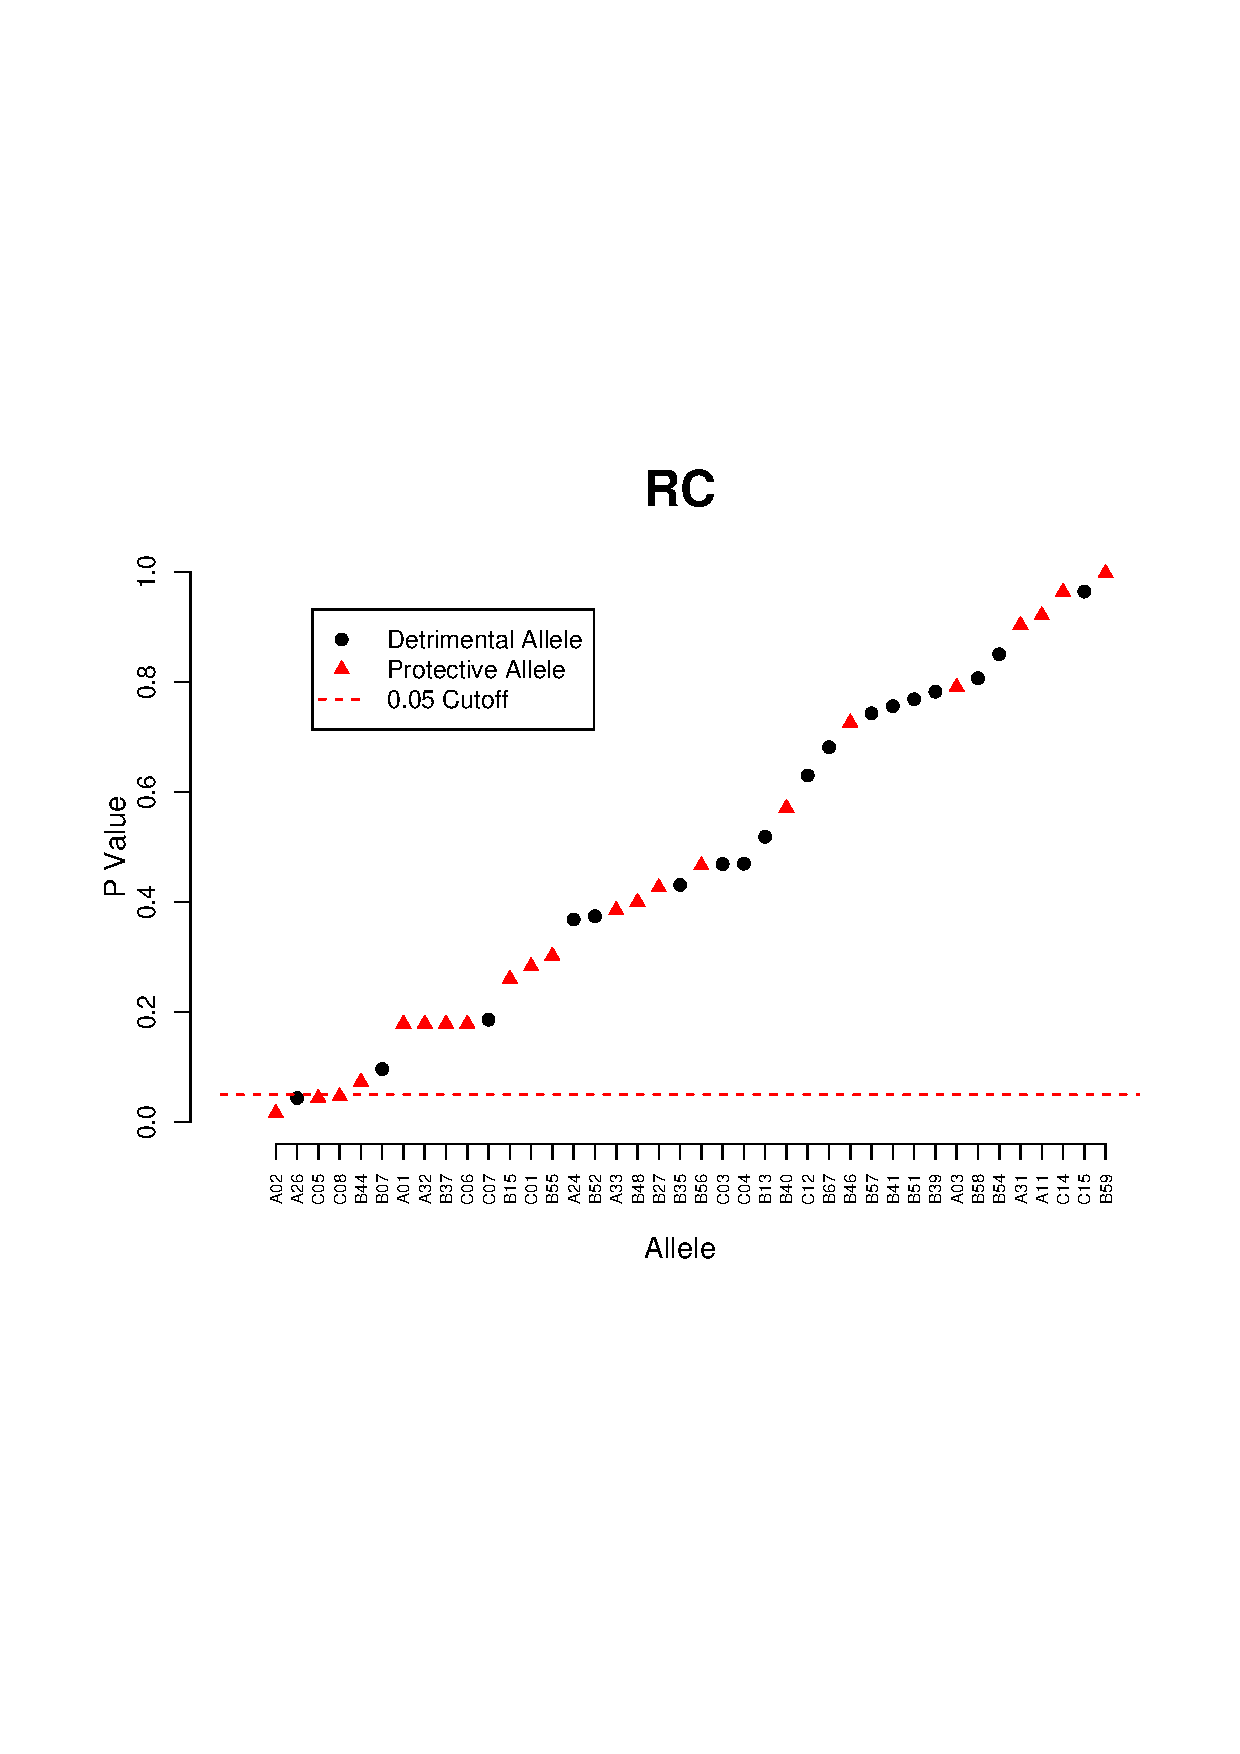
\includegraphics[width=14cm]{./Figures/chapter3/figureWilcoxAC}
\caption[Allele rankings for proviral load association]{The allele population of the HAM/TSP and AC individuals ranked by their Mann-Whitney $U$-test $P$ values, as described in \sref{chapter3/methodsLoad}. The black circle indicates that the association is negative (the presence of the allele is associated with a higher proviral load) and the red triangle indicates a positive association.}
\label{chapter3/figureLoad}
\end{figure}

\begin{figure}[htp]
\centering
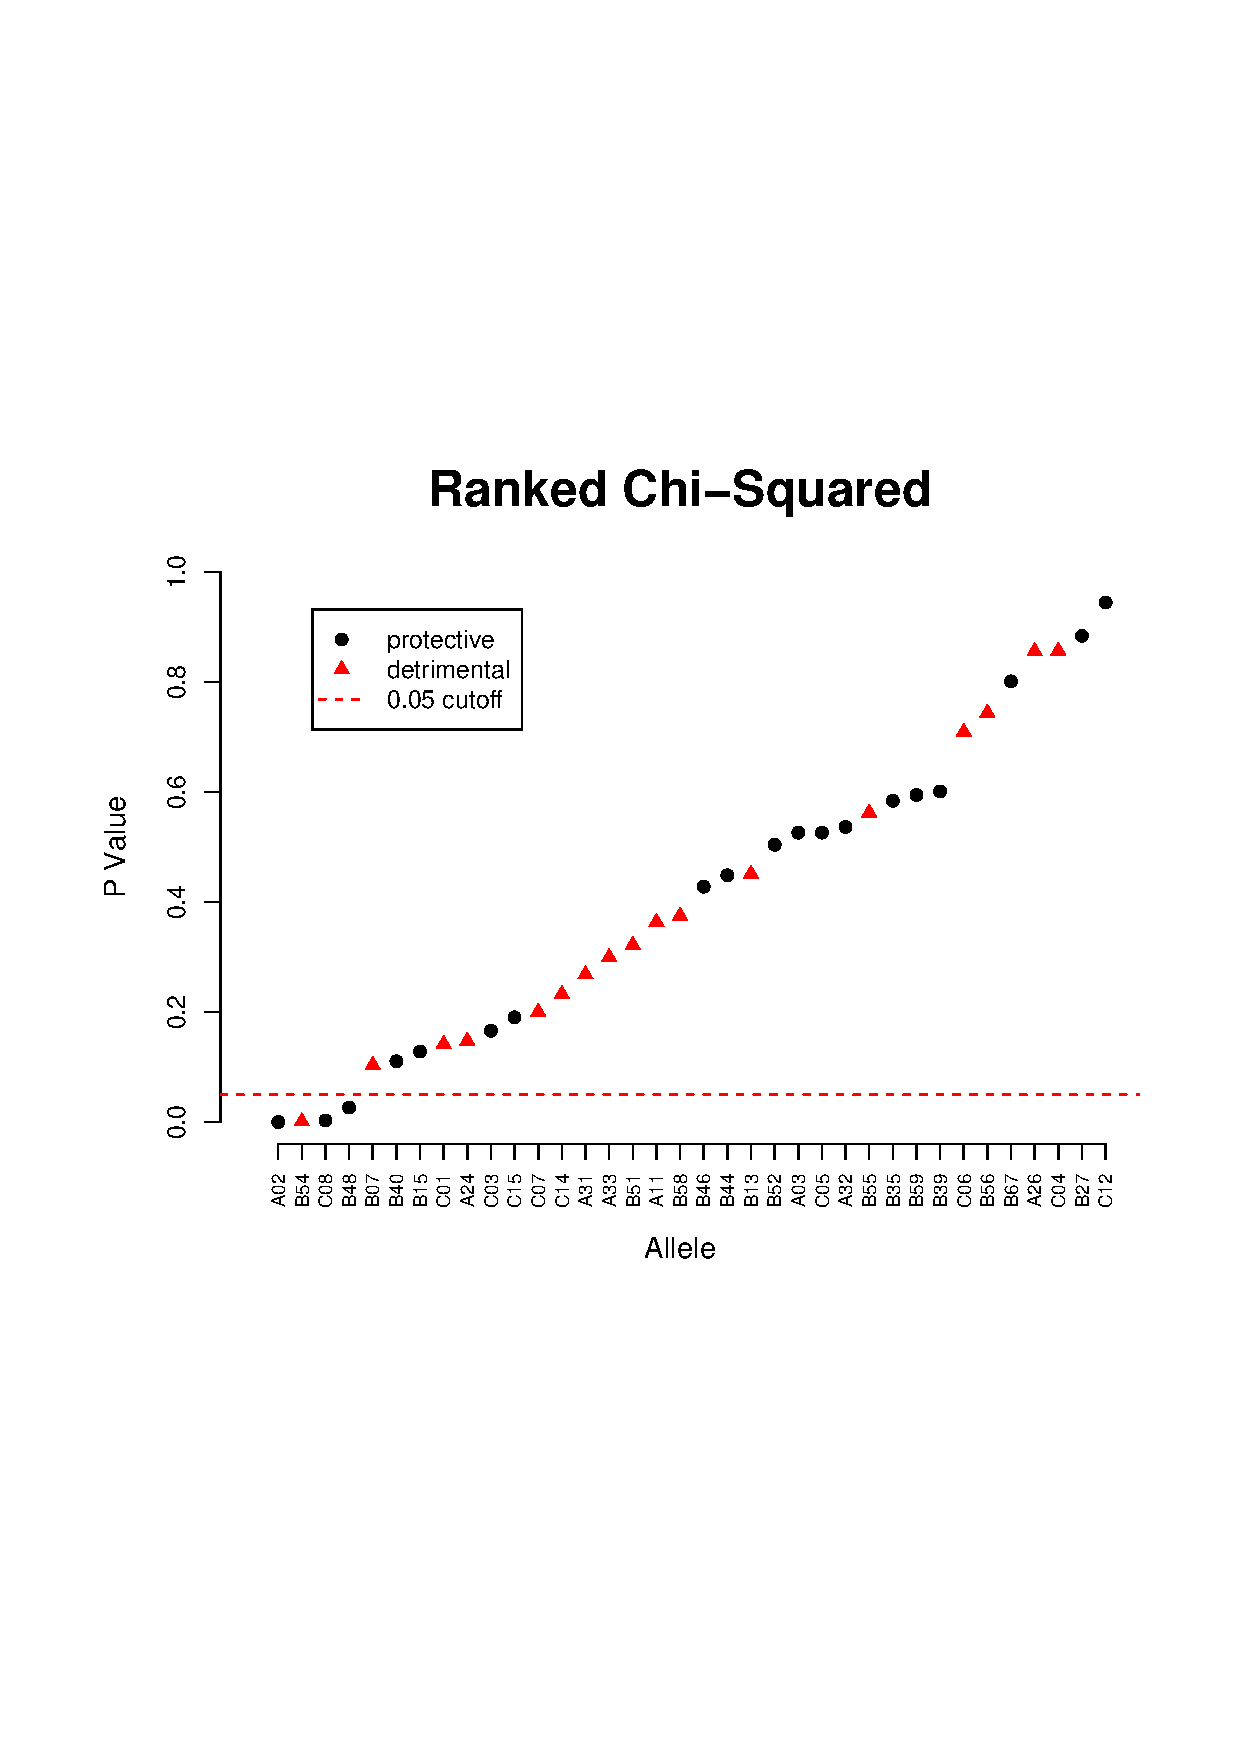
\includegraphics[width=14cm]{./Figures/chapter3/figureChi}
\caption[]{The result of the Yates $\chi^2$ analysis of disease risk for all alleles in the Kagoshima population. The black circles indicate a protective effect of an allele, the red trangle a detrimental effect. The red dotted line represents significance at $P = 0.05$.}
\label{chapter3/figureChi}
\end{figure}

\begin{figure}[htp]
\centering
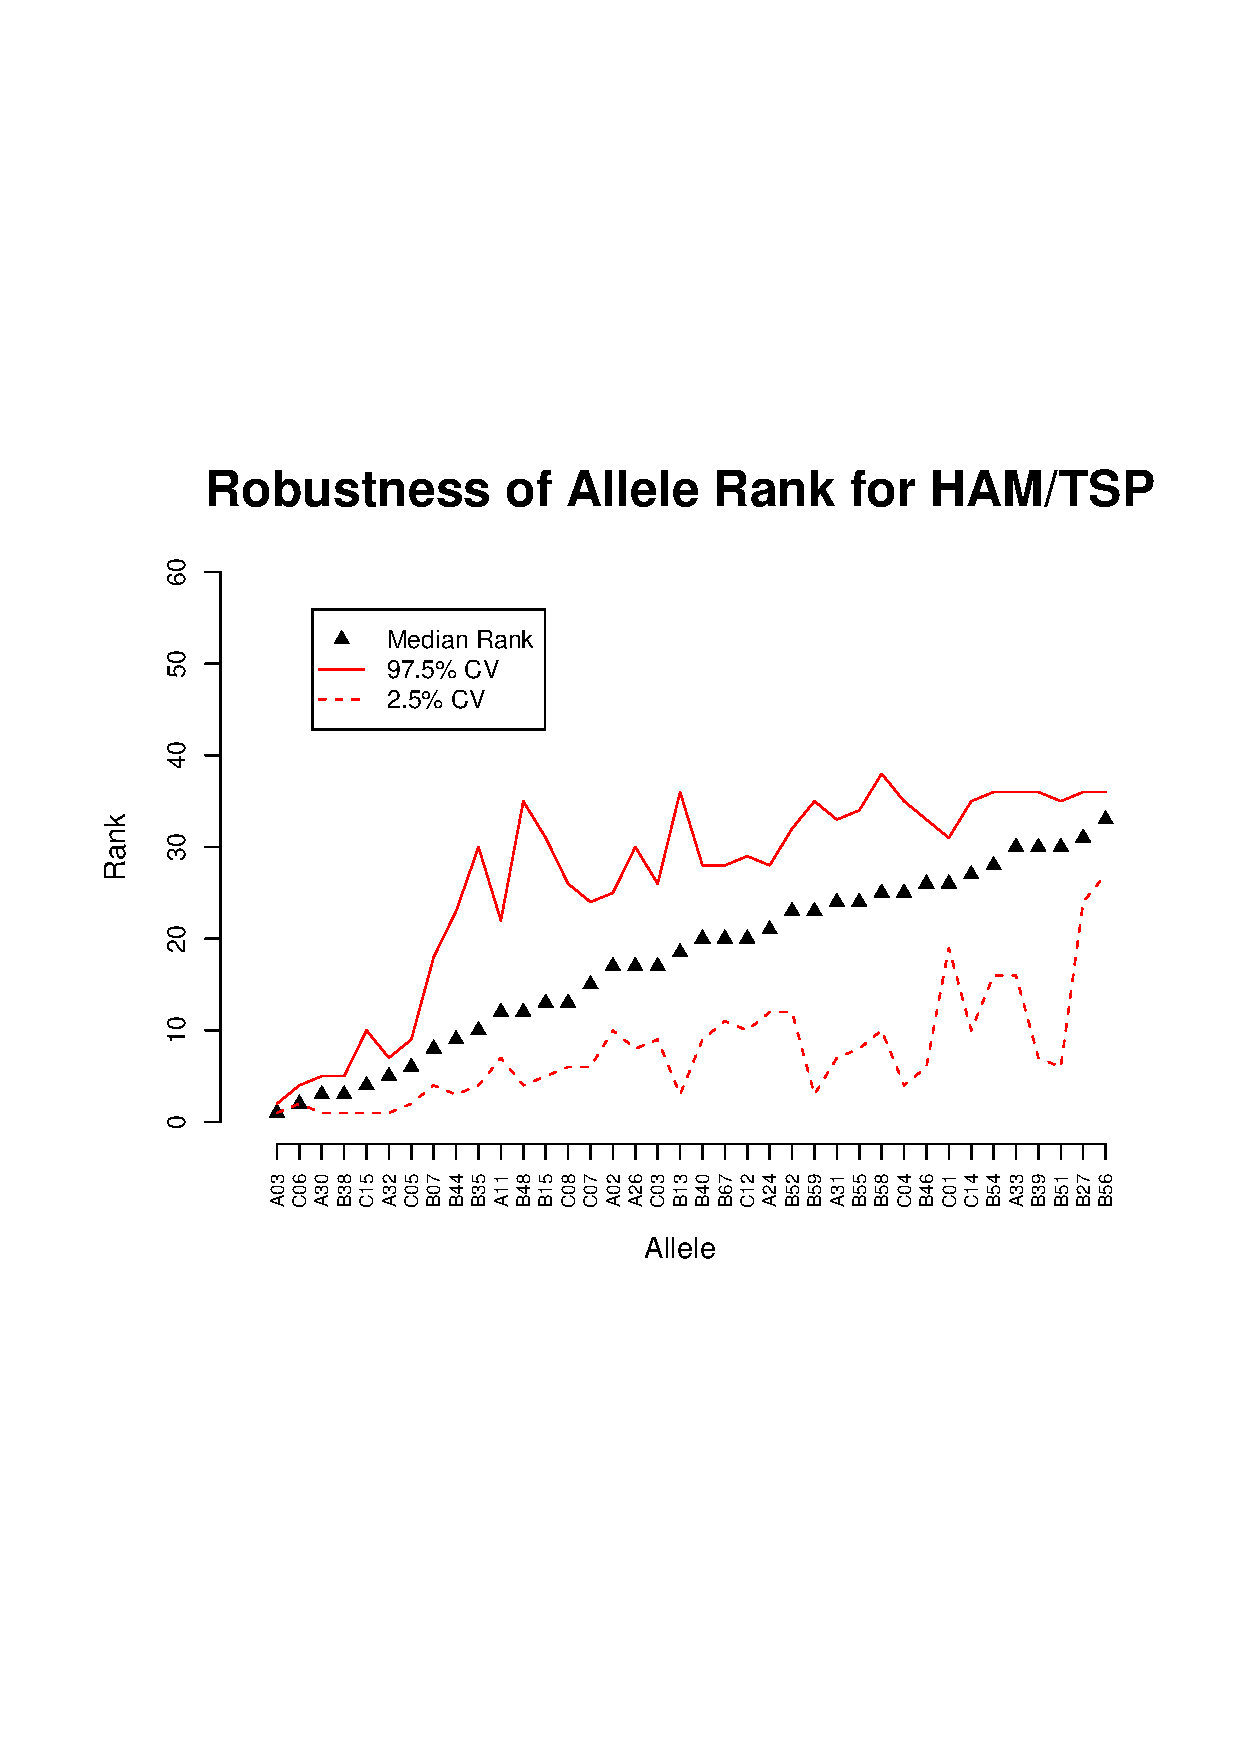
\includegraphics[width=14cm]{./Figures/chapter3/figureRobustHAM}
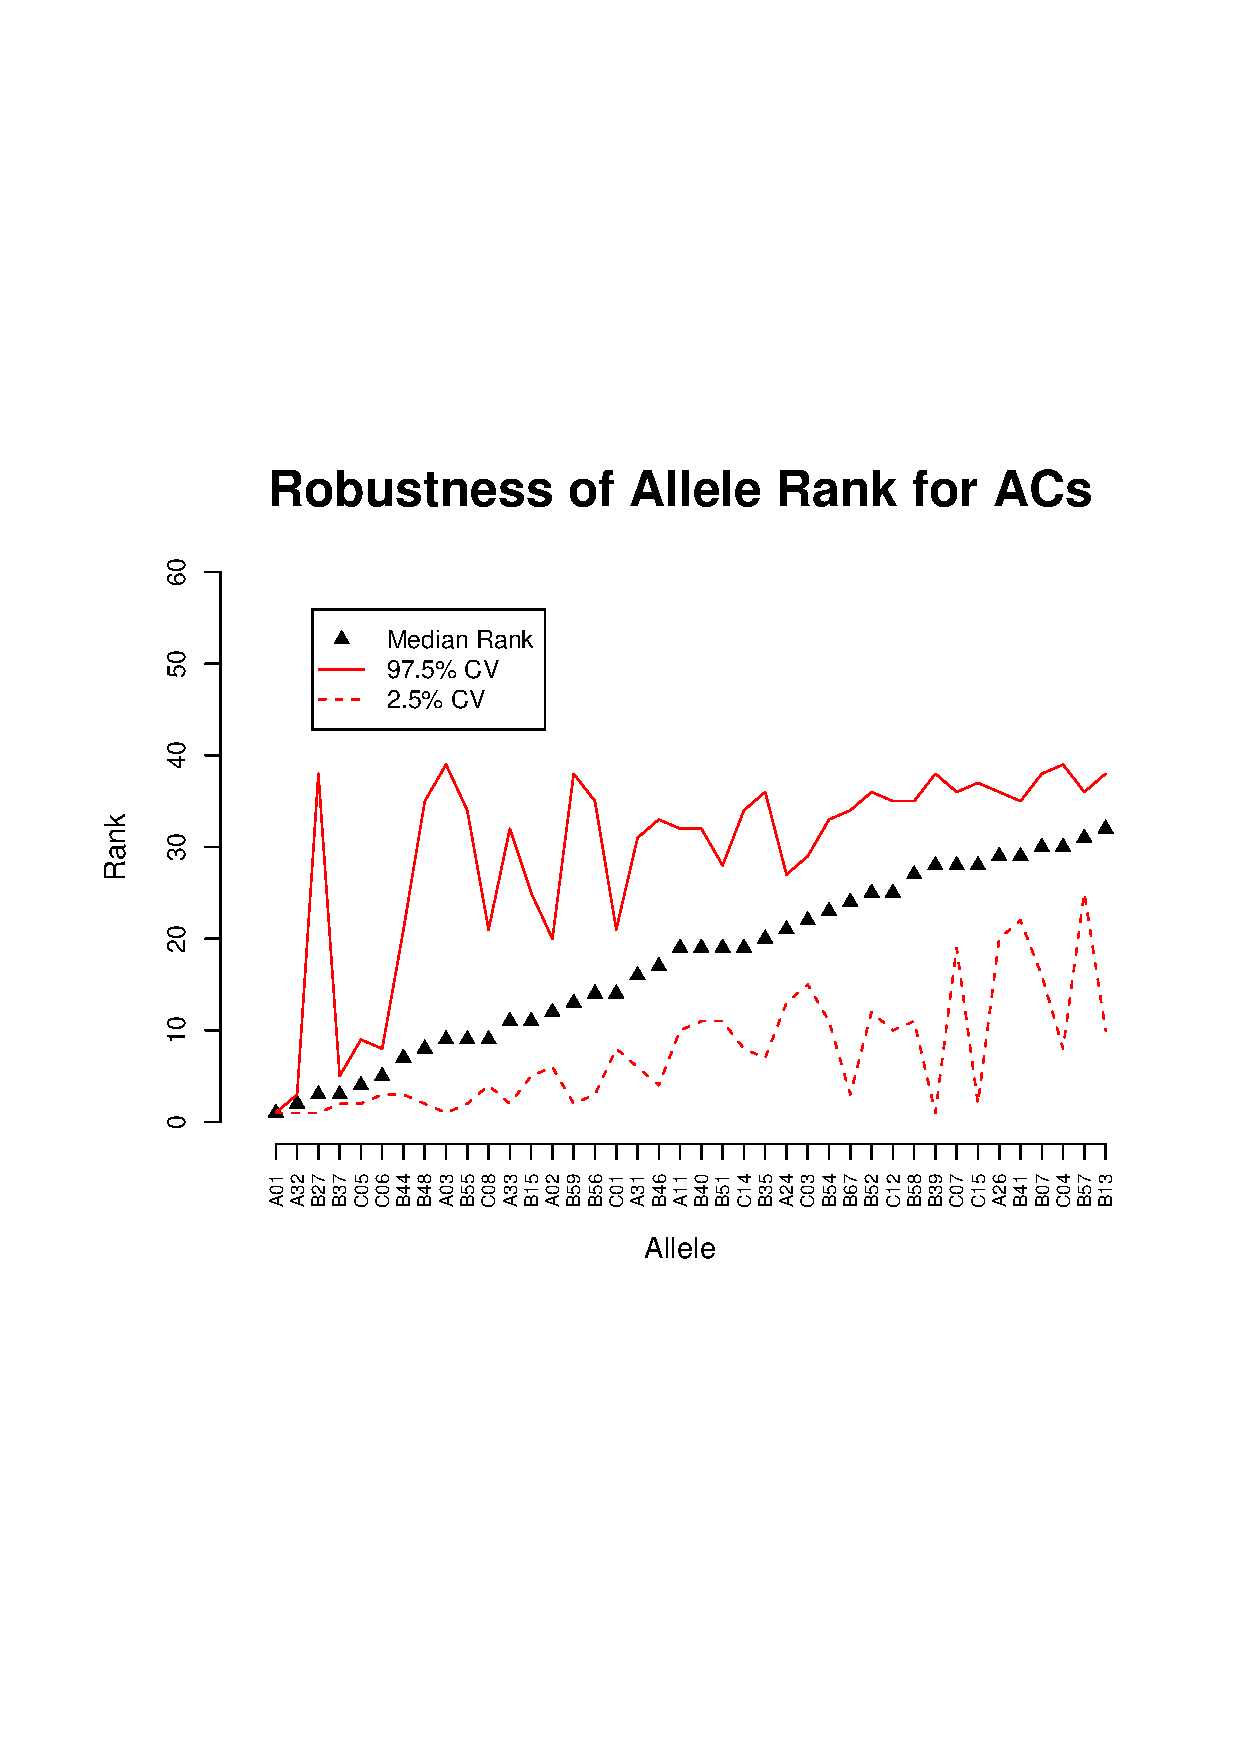
\includegraphics[width=14cm]{./Figures/chapter3/figureRobustAC}
\caption[The robustness of allele ranks]{The allele rankings and robustness, as described in \sref{chapter3/methodsLoad}. Each point gives the allele�s median rank over 2,000 iterations. The area between the solid dot and dotted lines gives the 95\% confidence interval of the value}
\label{chapter3/figureRobust}
\end{figure}

\section{Discussion}\label{chapter3/discussion}

Previous studies have clearly demonstrated the protective effect of \gene{Cw*08} and \gene{A*02} in terms of proviral load in aymptomatic carriers and disease risk \citep{Jeffery1999, Jeffery2000}. This would suggest a protective effect of a strong CTL response. The finding that heterozygosity also resulted in a significantly reduced proviral load suggested the presence of other protective alleles. We reanalysed the Kagoshima Cohort to look for any other allele effects with the goal of assembling the alleles of the cohort into larger sets of protective and detrimental alleles in order to give our epitope analysis greater power. 

\tref{chapter3/tableSummary} gives the summary of results for the tests of association between each allele in the Kagoshima Cohort against disease risk and proviral load. Using this combination of tests, we looked for any alleles that were significantly associated with either detrimental or protective outcomes, excluding those already known. From this analysis, no new alleles could be significantly linked with either disease status or proviral load. There are multiple reasons why this could happen: certain alleles may not have been represented at a high enough frequency in the Kagoshima cohort. More specifically, each individual expresses 6 co-dominant MHC class I alleles, which makes it a statistically difficult task to understand each allele's effect at the individual level. For example, the effect of possessing both detrimental and beneficial alleles may be additive or dominant in either direction. 
%(we specifically explore this question in \aref{AppendixC}, \sref{appendixc/AlleleEffect}).
We decided at this point to proceed with our definition of beneficial and detrimental alleles limited to \gene{Cw*08}/\gene{A*02} and \gene{B*54} respectively. By using epitope prediction software each allele could be clearly defined in terms of their epitope properties - a definition that takes into account funtionality and would be a more nuanced method of separating alleles compared to  their association with disease risk and proviral load. This analysis follows in \cref{Chapter4} and \cref{Chapter6}.	% Statistical Methods
% Chapter 4

\chapter{Rescaling in T-cell Epitope Prediction}
\label{Chapter4}
\lhead{Chapter 4. \emph{Rescaling in T-cell Epitope Prediction}}

\section{Introduction}\label{chapter4/introduction}

An ideal method to test hypotheses about the protective effect of MHC Class I alleles against disease risk and proviral load in HTLV-I would be to establish experimentally the HTLV-I peptides that bind to these protective and detrimental alleles. Unfortunately, very few MHC Class I epitopes have been experimentally confirmed for HTLV-I, unlike, for example, HIV \citep{LosAlamos2010}. Given the scarcity of available epitope information, it was necessary to use epitope-prediction software to predict the HTLV-I peptides that binded to the alleles of the Kagoshima Cohort. Before beginning the analaysis of HTLV-I, it was necessary to test the accuracy of these prediction methods outlined in \sref{Introduction/Prediction}, namely NetMHC v3.0 and NetCTL v1.2. During the course of this initial testing, our attention was drawn to a normalisation procedure - rescaling - that is used to compare the predicted binding affinities across different allleles. From this data, we wanted to test the hypothesis that rescaling predicted binding affinities results in a loss of allele-specific information and ultimately produces less accurate results in defining the epitope repertoire of HTLV-I. 

In order to make the prediction values comparable between each MHC molecule, it is recommended that the MHC-peptide binding affinity scores are rescaled \cite{Sturniolo1999}; this is explicitly implemented in NetCTL. The method of rescaling involves obtaining the predicted binding affinities of 500,000 random natural peptides for each MHC allelic predictor. From these affinities, a rescale value is calculated, defined as the binding affinity that is the threshold for the top 1\% of total binding affinities. The rescaled affinity is then defined as the predicted affinity score divided by this rescale value \citep{larsen2005}. Hence, from this calculation, all alleles are predicted to bind the same number of high-affinity peptides. One pragmatic reason for rescaling is to correct for any discrepancies between the allelic predictors that resulted from inconsistent training data (e.g.~data that came from different sources), by assuming that all alleles should bind the same number of epitopes (C.~Ke\c{s}mir, pers.~comm.). Additionally, there are biological arguments for believing that different alleles should bind similar numbers of epitopes. It has been postulated that the opposing constraints of effective pathogen recognition but tolerance of self would result in a very narrow range of optimal promiscuity for viable MHC class I molecules. A narrow range of promiscuity would also be predicted as a direct outcome of effective tapasin-dependent peptide optimization in the endoplasmic reticulum \citep{George2005, Elliott2006, Williams2002}.

However, we will present evidence in this chapter that in correcting for differences between the allelic predictors, information is being lost that reflects true biological variation between MHC molecules and, by extension, differences in their ability to bind to peptide sequences. We show that, for both qualitative and quantitative measures of binding, rescaling impairs rather than improves allelic predictor performance. This is of importance for vaccine design and to understand the nature of the CTL response. In particular, crucial between-allele variations in binding affinity and preference which may contribute to differences in the outcome of infection are likely to be obscured by rescaling.

\section{Methods}

\subsection{Prediction Method Outputs}

In order to test the effect of rescaling on epitope prediction accuracy, we used two web-based prediction methods, NetCTL v1.2 \citep{larsen2005} and NetMHC v3.0 \citep{buus2003, nielsen2003, nielsen2004}. NetCTL is an integrated method that uses information pertaining to TAP and protein cleavage in its predictions, together with MHC binding. The output is combined by rescaling the MHC binding result and adding this to the weighted scores for TAP and protein cleavage. NetCTL has allelic predictors for 12 different class I alleles that are chosen to be representative of each of 12 supertypes; hence it has 12 different rescaling factors.

NetMHC v3.0 simply predicts MHC-peptide binding, using ANNs to predict binding affinities for 43 MHC molecules. In order to test the effect of rescaling, it was necessary to produce rescale values for each of the 43 allelic predictors. This was performed as in NetCTL; 500,000 unique random nonamers were obtained from the proteome of \emph{Mycobacterium tuberculosis}, their binding affinity was predicted and the rescale value (top percentile) was found for each allelic predictor. We also performed this calculation with 500,000 random natural peptides to test for the possibility of error from bias in amino acid usage in \emph{Mycobacterium tuberculosis}. There was no significant difference in the rescale values obtained using these two different sources (\fref{chapter4/rescaleValues}). 

In summary, we tested two sets of rescaling values: those obtained from NetCTL v1.2 and those that we calculated using NetMHC v3.0.

\subsection{Datasets}\label{chapter4/methodsDatasets}

Epitope datasets were constructed from sources detailed below. In each case, the prediction methods were tested by their ability to detect these epitopes amongst the full set of overlapping nonamers derived from the proteins that contained the epitopes. The full set of nonamers will contain a small number of known epitopes and the remainder will be `non-epitopes'. Of course, this set of non-epitopes could include epitopes that have not been experimentally verified. However, the majority (see \sref{chapter4/introduction}) would be non-binders with the corresponding MHC molecule. Added to this, the labelling of epitopes as `non-epitopes' impact on both rescaled and non-rescaled calculations equally. Previous research has also shown that this property of the `non-epitope' set did not produce significantly different results \citep{heckerman2007}. Each respective set of experimentally defined epitopes was denoted the positive dataset and the set of non-binding (or unknown) peptides was denoted the negative dataset.

\subsubsection{The SYF$^1$ Dataset}\label{chapter4/methodsSYF1}

The SYF1 dataset is a supertype dataset derived from SYFPEITHI \citep{rammensee1999} and is identical to that used in the original paper for NetCTL \citep{larsen2005}. Each epitope in SYF$^1$ was experimentally verified to bind to one of 10 MHC class I supertypes \citep{Sette1999}. The resulting dataset consisted of 148 epitope-supertype pairs. The corresponding negative dataset was obtained by concatenating the SwissProt entry proteins from which each of the epitopes was derived. The length of the concatenated protein sequence was 78,259 amino acids. The ROC curve (\sref{chapter4/methodsROC}) was generated using a negative set of $\big( \left( 78,259 \times 10 \right) - 148 \big) = 782,442$ nonamers and a positive set of 148 nonamers. The positive set of SYF$^1$ is available in \aref{AppendixA}, \tref{appendixa/table1}.

\subsubsection{The Lanl$^{661}$ Dataset}\label{chapter4/lanl661}
 
Experimentally defined epitopes in HIV-I were extracted from the HIV Molecular Immunology Database \citep{Bette2005}. In total, 1,618 CTL epitopes were found that were bound by human MHC molecules. However, this set was highly redundant; the epitope lengths were variable and a large number of epitopes differed only by mutations within the sequence. Also, resolution of their MHC typing varied from 2 to 4 digits. To correct for this variability, a number of changes were made to the MHC allele-epitope list. Firstly, all MHC alleles were defined to two digits. Secondly, variant epitopes binding the same allele were discarded. Finally, as the prediction software only produced binding predictions for nonamer epitopes, all epitopes that were not 9 amino acids long were removed from the list.

In summary, it was possible to test 41 of the 43 allelic predictors for MHC molecules in NetMHC v3.0. The positive set consisted of 661 epitopes, defined in terms of start and end positions relative to the HIV reference strain HXB2 (\aref{AppendixA}, \tref{appendixa/HXB2}) and a matching MHC type to 2 digits. The input protein sequence to NetMHC contained 3,000 overlapping nonamers that covered the proteome from which the whole positive set of epitopes was derived. The total `negative set' for the ROC analysis was $\big( \left( 3,000 \times 41 \right) - 661 \big) = 122,339$ nonamers, and a positive set of 661 nonamers. The positive set of Lanl$^{661}$ is available in \aref{AppendixA}, \tref{appendixa/table3}.

\subsubsection{The Lanl$^{179}$ Dataset} 

The Lanl$^{661}$ dataset was modified for testing with NetCTL. From these 661 epitopes, a total of 179 bound to the 12 alleles for which NetCTL has allelic predictors. The input sequence to NetCTL contained 3,000 overlapping nonamers. For this experiment, the negative set consisted of $\big( \left( 3,000 \times 12 \right) - 179 \big) = 35,821$ nonamers, and a positive set of 179 nonamers. The positive set of Lanl$^{179}$ is available in \aref{AppendixA}, \tref{appendixa/table2}.

\subsection{ROC Curves}\label{chapter4/methodsROC} 

ROC curves give a visual measure of the accuracy of a prediction method. The threshold at which the prediction method identifies a peptide as being an epitope varies along the length of the curve. Each point on the curve gives the fraction of true positive epitopes found as a function of the number of false positive `epitopes' at that threshold. Hence, setting a strict threshold for epitope detection will result in high specificity (correct predictions) but low sensitivity (missing a high proportion of true binders). The area under the ROC curve gives the AUC (Area under Curve) measurement. In order to test for significant difference between ROC curves, we conducted the bootstrapping analysis detailed in \citep{Peters2006}. Briefly, using bootstrapping with replacement, 100 replicates were formed from each dataset and the resulting non-rescaled and rescaled whole AUC values were compared using a paired $t$-test.

\subsection{Other Measurements of Performance}

Using the 2 epitope datasets, HIV$^{216}$ and SYFPEITHI$^{863}$, and the same methods from \citep{larsen2007}, we repeated 3 of the measurements described in that paper for the rescaled and non-rescaled results of NetCTL v1.2. For the Rank measure, we analysed the proteins from which each epitope was derived. For each protein, we calculated the rank of the epitope amongst all overlapping 9-mers using rescaling and non-rescaling scoring methods for all alleles. We then analysed these ranks to see which method ranked the epitopes higher. For the second method, we measured the specificity of both rescaling and non-rescaling at predefined sensitivities. Finally, we measured the sensitivity among the top 5\% top-scoring peptides, again for the rescaled and non-rescaled binding affinities. 

\subsection{Other Data Sources}

The training data for NetMHC v3.0 is available at the Immune Epitope Database and Analysis Resource (\href{http://mhcbindingpredictions.immuneepitope.org/}{\texttt{IEDB}}). An independent set of experimental epitope-allele binding affinities was obtained from IEDB by selecting all experimental data that did not originate from the laboratories of Sette \emph{et al.}~or Buus \emph{et al.}~(the training data originated from these two sources).

%%%%%%%%%%%%%%%%%%%%%%%%%%%%%%%%%%%%%%%%%%%%%%%%%%%%%%%%%%%%%%%%%%%%%%%%%%%%%%%%%%%%%%%%%%%%%%%%%%%%

\section{Results}\label{chapter4/results}

\subsection{The Effect of Rescaling on Qualitative Epitope Prediction}

ROC curves were used to analyse the effects of rescaling on epitope prediction. Both NetCTL v1.2 and NetMHC v3.0 were tested and 3 datasets were used (\fref{chapter4/figure1} and \tref{chapter4/table1}). In each case, rescaling resulted in a significant loss of performance (bootstrap test: $P < 0.001$).

\begin{table}[tbp]
\centering
\begin{sideways}
\begin{tabulary}{\textwidth}{|l|l|l|l|l|l|l|}
\hline
ROC Curve & Colour & Method & Dataset & Rescaling & AUC 30\% & Bootstrap $P$ Value \bigstrut \\
\hline
\multirow{2}{*}{\fref{chapter4/figure1} A} & Black Solid & NetCTL v1.2 & SYF$^1$ & No & 0.949 & \multirow{2}{*}{$P < 0.001$} \bigstrut[t] \\
& Red Dashed & NetCTL v1.2 & SYF$^1$ & Yes & 0.937 & \bigstrut[b] \\
\hline
\multirow{2}{*}{\fref{chapter4/figure1} B} & Black Solid & NetMHC v3.0 & SYF$^1$ & No & 0.932 & \multirow{2}{*}{$P < 0.001$} \bigstrut[t] \\
& Red Dashed & NetMHC v3.0 & SYF$^1$ & Yes & 0.905 & \bigstrut[b] \\
\hline
\multirow{2}{*}{\fref{chapter4/figure1} C} & Black Solid & NetMHC v3.0 & Lanl$^{661}$ & No & 0.944 & \multirow{2}{*}{$P < 0.001$} \bigstrut[t] \\
& Red Dashed & NetMHC v3.0 & Lanl$^{661}$ & Yes & 0.937 & \bigstrut[b] \\
\hline
\multirow{2}{*}{\fref{chapter4/figure1} D} & Black Solid & NetCTL v2.1 & Lanl$^{179}$ & No & 0.933 & \multirow{2}{*}{$P < 0.001$} \bigstrut[t] \\
& Red Dashed & NetCTL v2.1 & Lanl$^{179}$ & Yes & 0.918 & \bigstrut[b] \\
\hline
\end{tabulary}
\end{sideways}
\caption[ROC curve summary statistics]{The summary statistics and details of each ROC curve from \fref{chapter4/figure1}.}\label{chapter4/table1}
\end{table}

In NetCTL v1.2, the TAP and cleavage scores are combined with the rescaled MHC binding score to produce a combined score for each submitted nonamer. In order to test how NetCTL performed without rescaling, it was still necessary to divide the MHC binding score by a rescaling value so the weightings of the TAP and cleavage score were still applicable and accurate. By averaging over all rescaling values and dividing the MHC binding value by this number, rescaling differences were ``averaged out'' and it was still possible to use the extra information from the TAP and cleavage predictions.

\begin{figure}[htp]
\centering
\includegraphics[width=7cm]{./Figures/chapter4/figure_1A}%
\hspace{0cm}%
\includegraphics[width=7cm]{./Figures/chapter4/figure_1B} \\
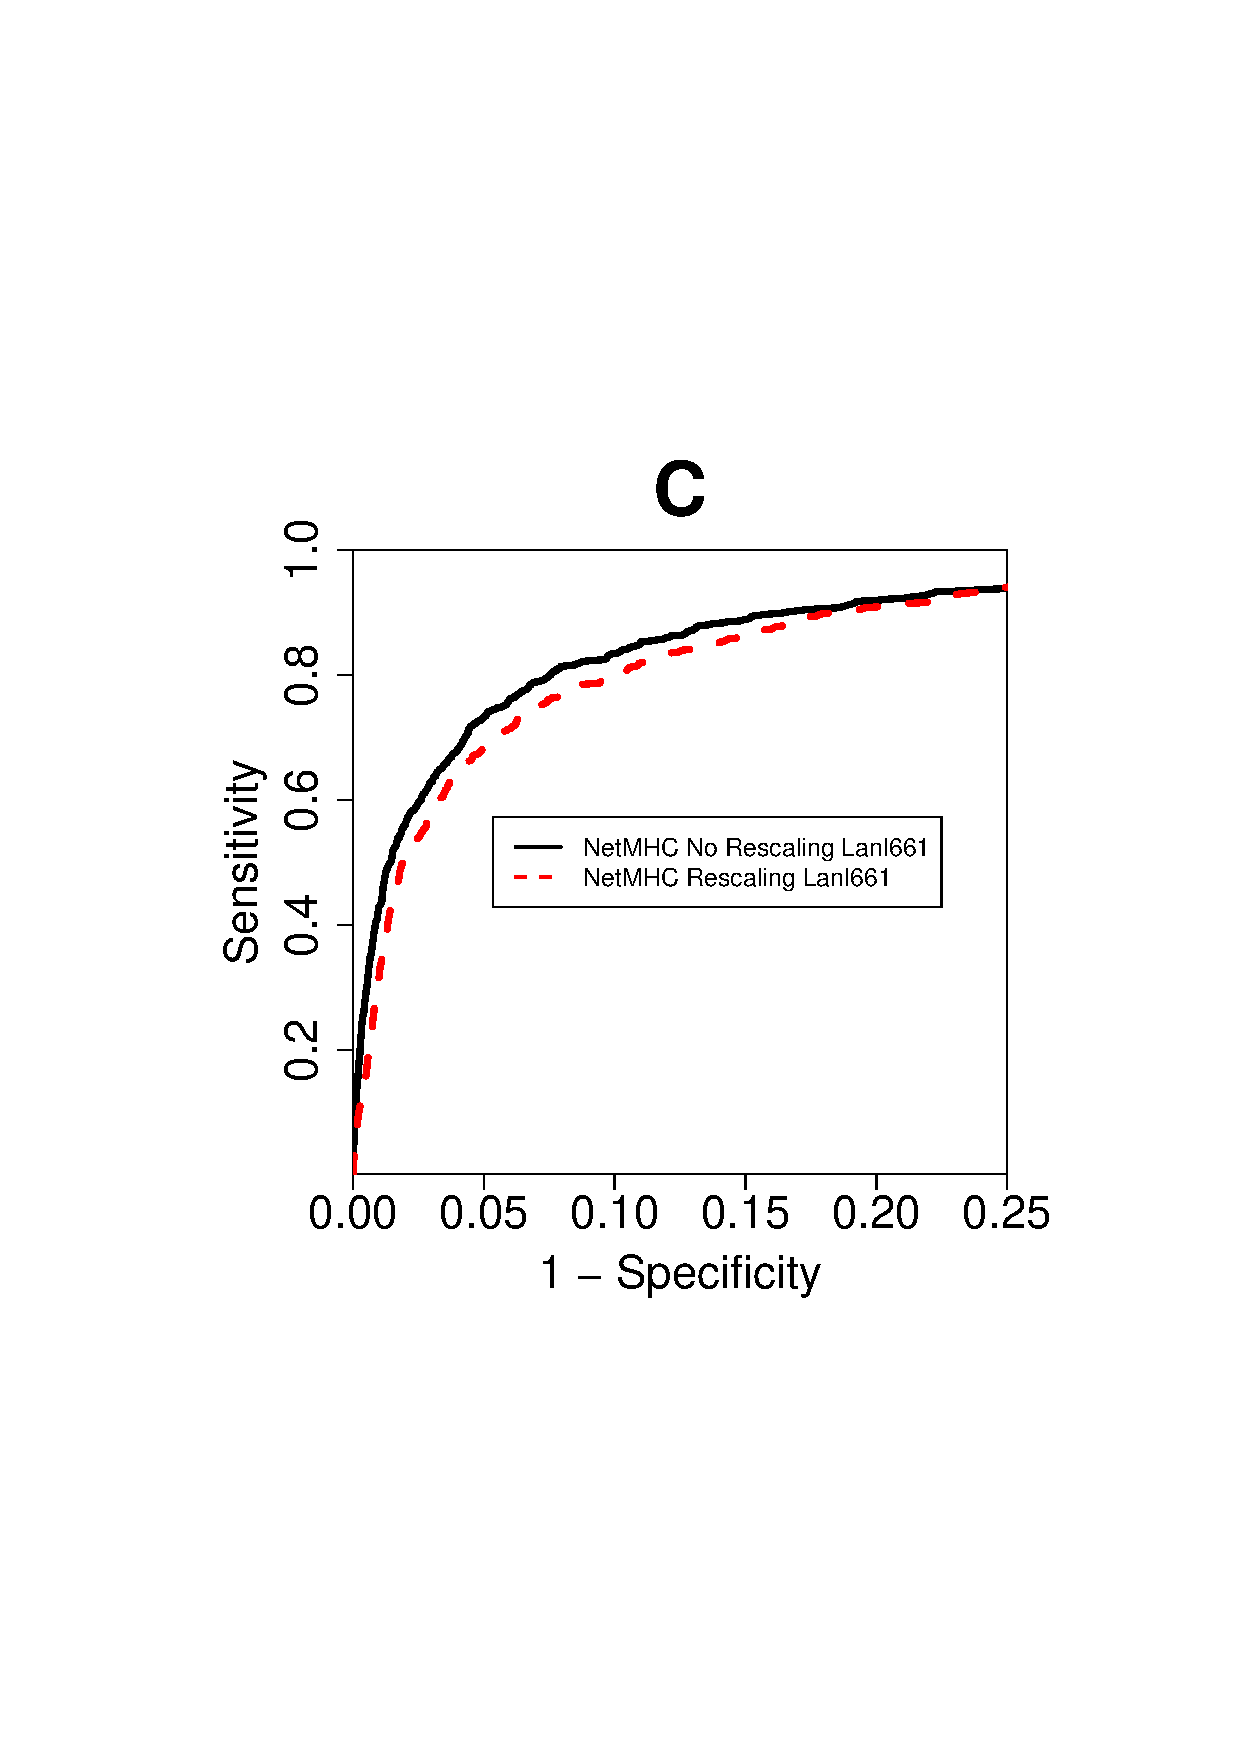
\includegraphics[width=7cm]{./Figures/chapter4/figure_1C}%
\hspace{0cm}%
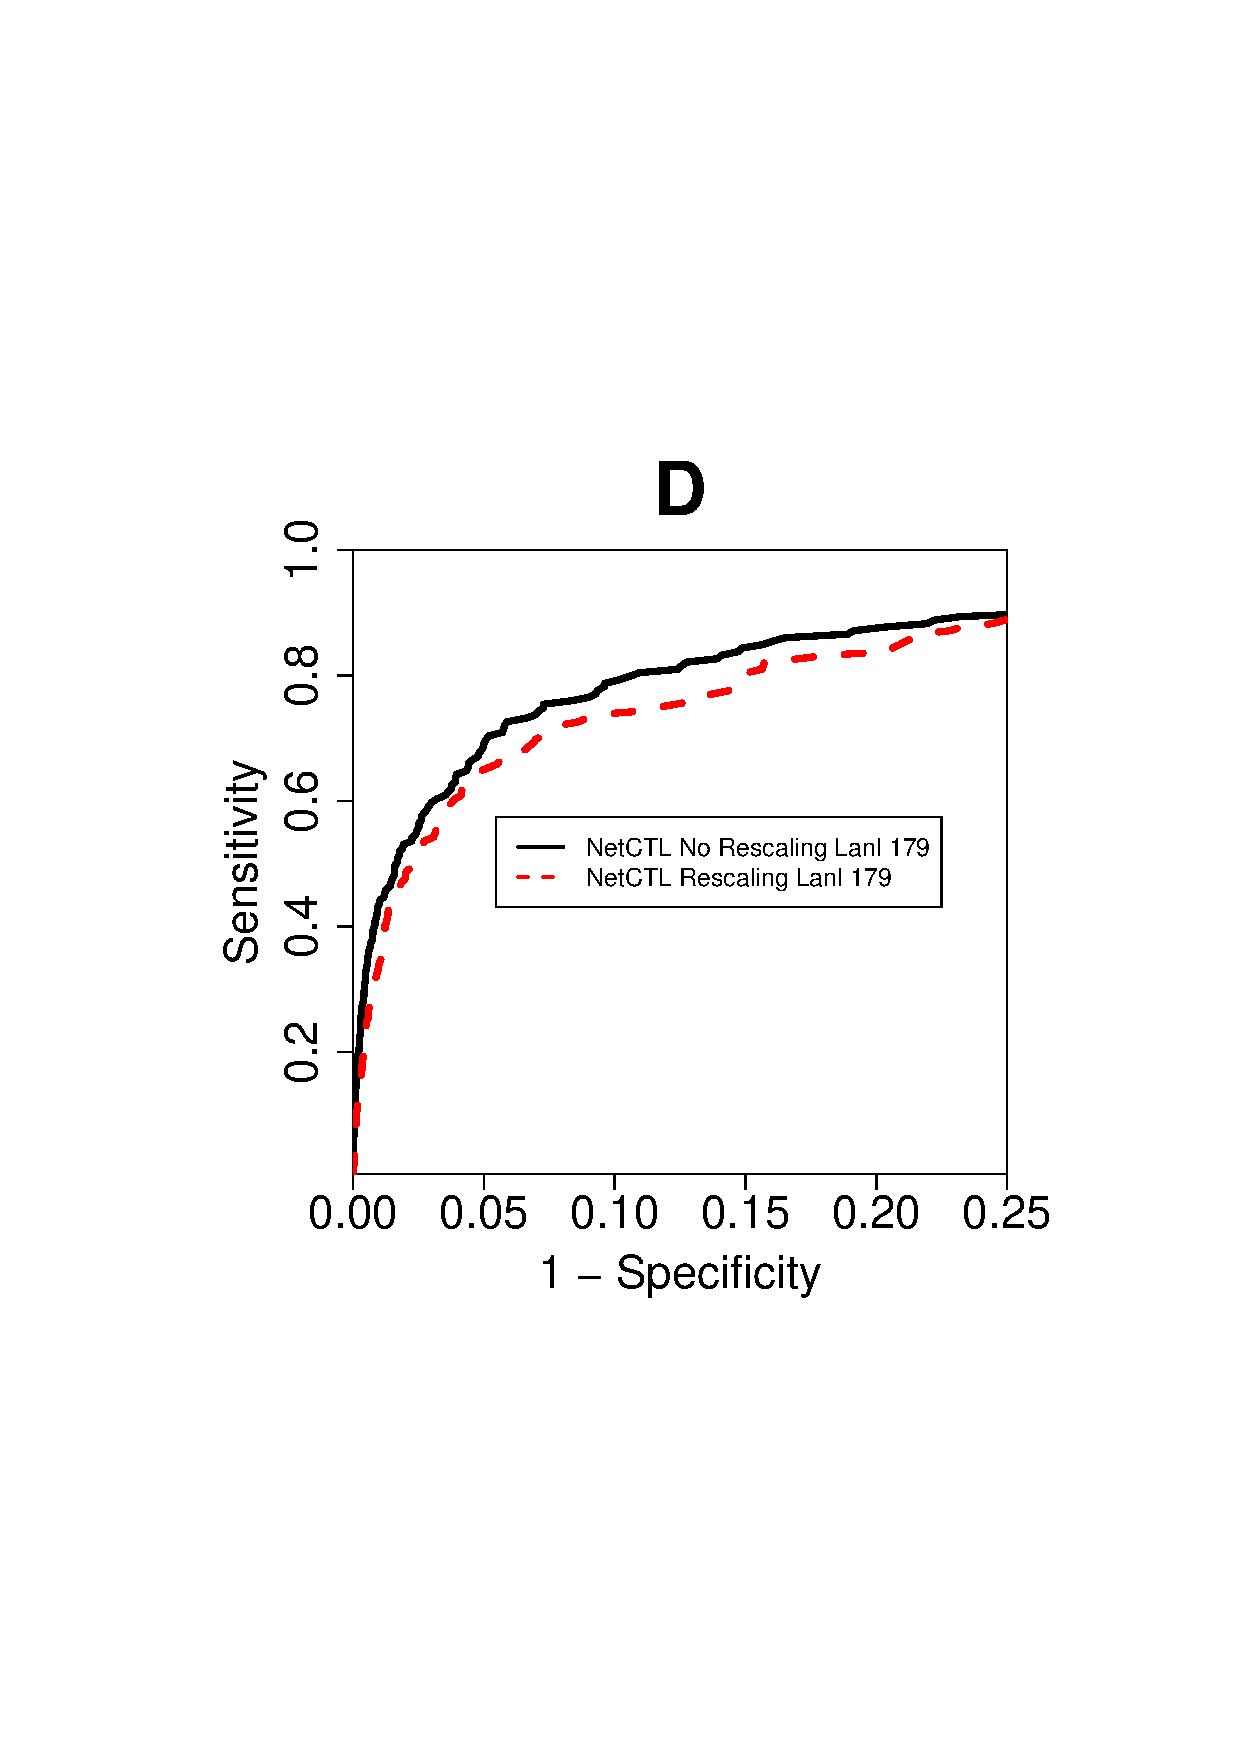
\includegraphics[width=7cm]{./Figures/chapter4/figure_1D} \\
\caption[The ROC curves comparing rescaling and non-rescaling]{Each graph shows the ROC curves using different combinations of datasets and prediction methods (see \tref{chapter4/table1}). A uses NetCTL with the SYF$^1$ dataset, B uses NetMHC with the SYF$^1$ dataset, C uses NetMHC with the Lanl$^{661}$ dataset and D uses NetCTL with the Lanl$^{179}$ dataset. The x-axis has been scaled to show the region of importance (the AUC with high specificity values). The rescaled results (red dashed line) are compared against non-rescaled (black solid line). \tref{chapter4/table1} gives the statistics for each graph.}
\label{chapter4/figure1}
\end{figure}

\subsection{Comparison of Rescale Values}

We calculated rescale values based on the predicted binding to 500,000 peptides selected at random from \emph{Mycobacterium tuberculosis}. To check that the source of the peptides did not alter our conclusions we randomly selected 500,000 natural peptides from the Swiss-Prot database \citep{Consortium2008} and produced the top percentile re-scaling values for each allele from these peptides. \fref{chapter4/rescaleValues} compares these values to the re-scaling values we previously used, which were derived from non-overlapping peptides from \emph{Mycobacterium tuberculosis}. As can be seen from \fref{chapter4/rescaleValues}, the two sets of rescale values are strongly positively correlated ($R^2 = 0.9563$, $P < 0.001$). Repeating our ROC curve analysis of rescaled and non-rescaled predictions from \fref{chapter4/figure1} C using these new rescale factors (\fref{chapter4/randomROC}) gives very similar results to those reported here. Consequently, whether we calculate the rescale factors using random natural peptides from \emph{Mycobacterium tuberculosis} or on random natural peptides from a range of proteins, our conclusions remain unchanged.

\begin{figure}[htp]
\centering
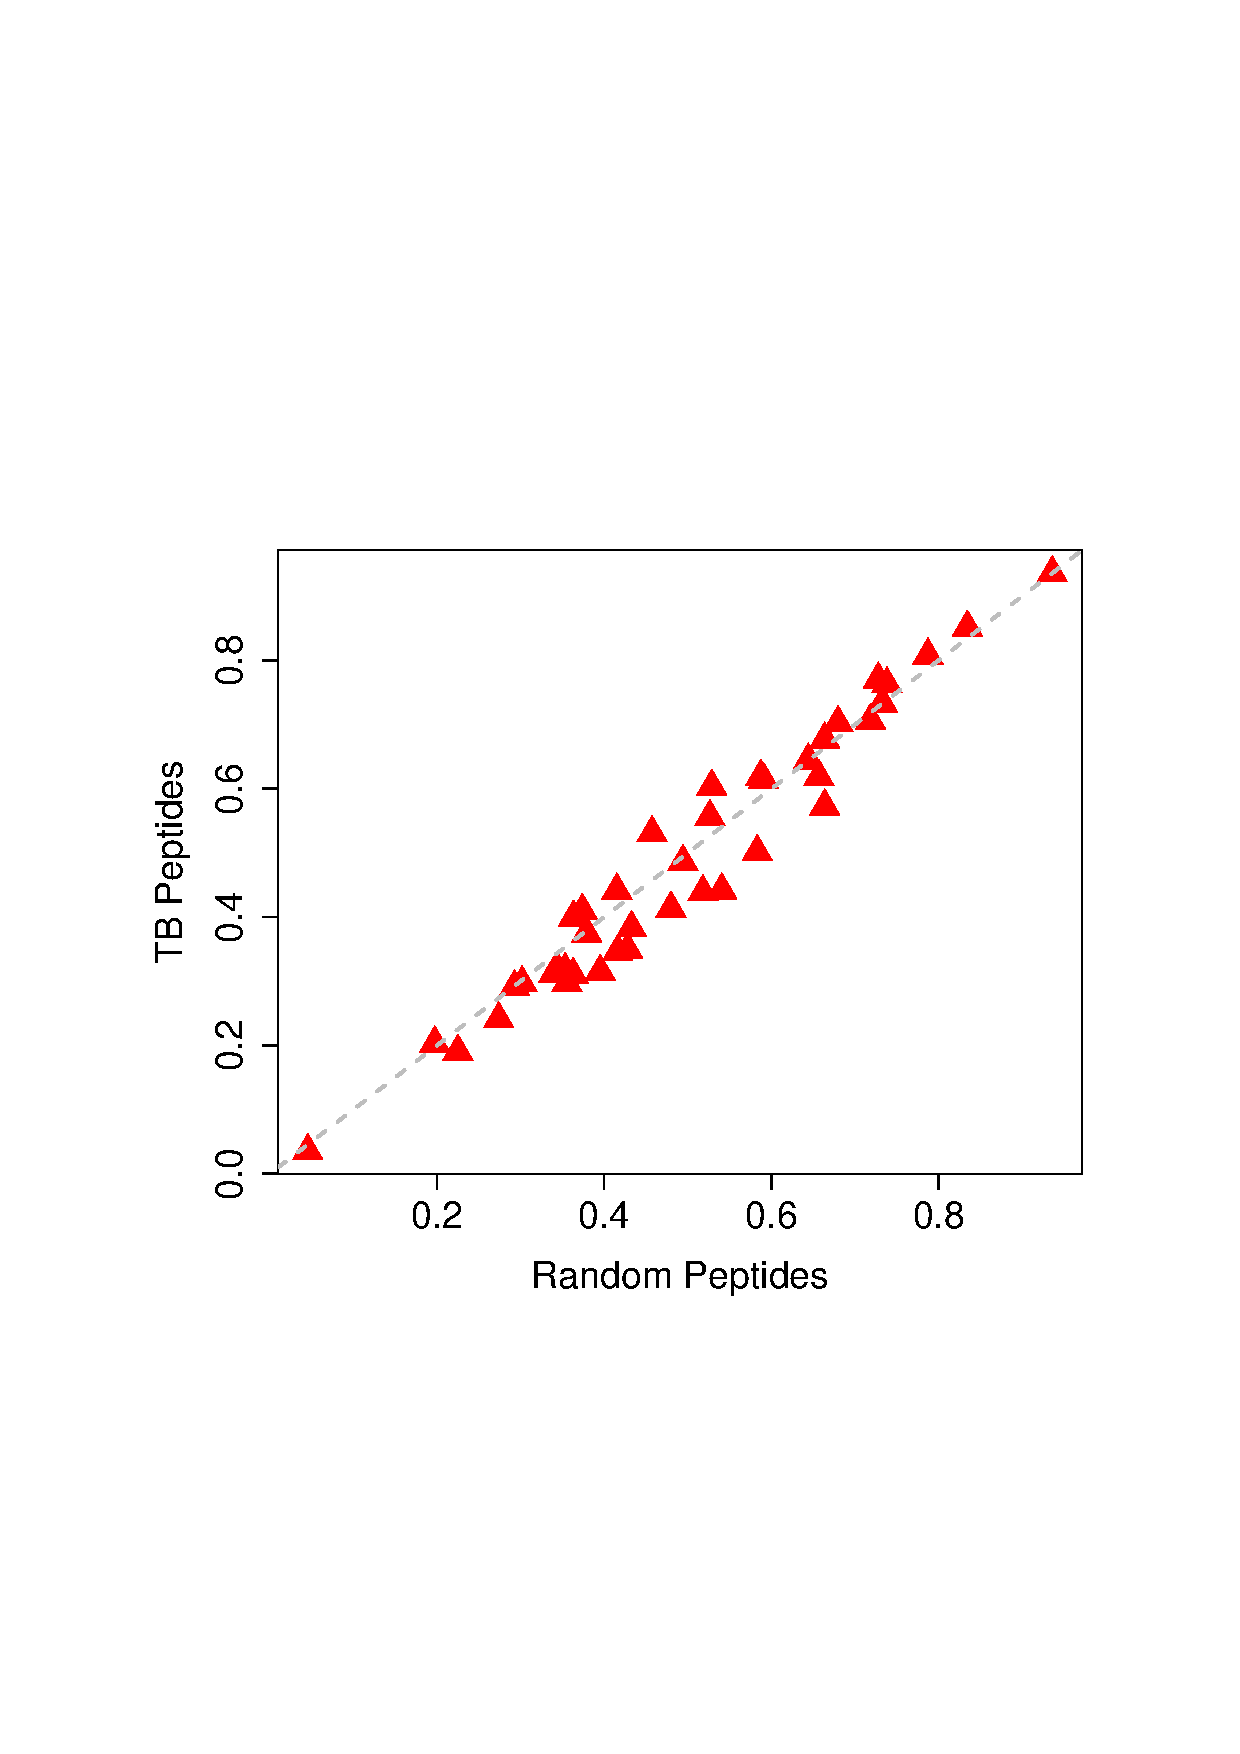
\includegraphics[width=14cm]{./Figures/chapter4/rescaleValues}
%\rule{35em}{0.5pt}
\caption[The relationship between rescale values]{The relationship for the top percentile rescaling values for each allele between random natural peptides and non-overlapping peptides from Mycobacterium tuberculosis. There was no significant difference between the two measures (Mann-Whitney paired test, $P = 0.1181$) and the data was strongly correlated ($R^2 = 0.9563$, $P < 0.001$).}
\label{chapter4/rescaleValues}
\end{figure}

\begin{figure}[htp]
\centering
\includegraphics[width=10cm]{./Figures/chapter4/randomROC}
%\rule{35em}{0.5pt}
\caption[The ROC curve analysis without with randomly derived rescale values]{The ROC analysis of the Lanl$^{661}$ dataset. The rescale values used are derived from random natural peptides, as opposed to peptides originating from \emph{Mycobacterium tuberculosis}. The difference remains significant between the two curves (bootstrap test: $P < 0.001$).}
\label{chapter4/randomROC}
\end{figure}

\subsection{Variation in Rescale Values as a Function of Accuracy}

One possible explanation for why rescaling has a detrimental impact on prediction is that there may be a positive correlation between rescale factor and allelic predictor accuracy (Morten Nielsen, pers.~comm.). To check this hypothesis we calculated the AUCs for each NetMHC v3.0 predictor using the Lanl$^{661}$ dataset and plotted this against the corresponding rescale factor, the results of which are shown in \fref{chapter4/figure2}. This shows no evidence of a correlation between rescaling values and the AUC values ($R^2 = 0.0068$, $P = 0.606$).

\begin{figure}[htp]
\centering
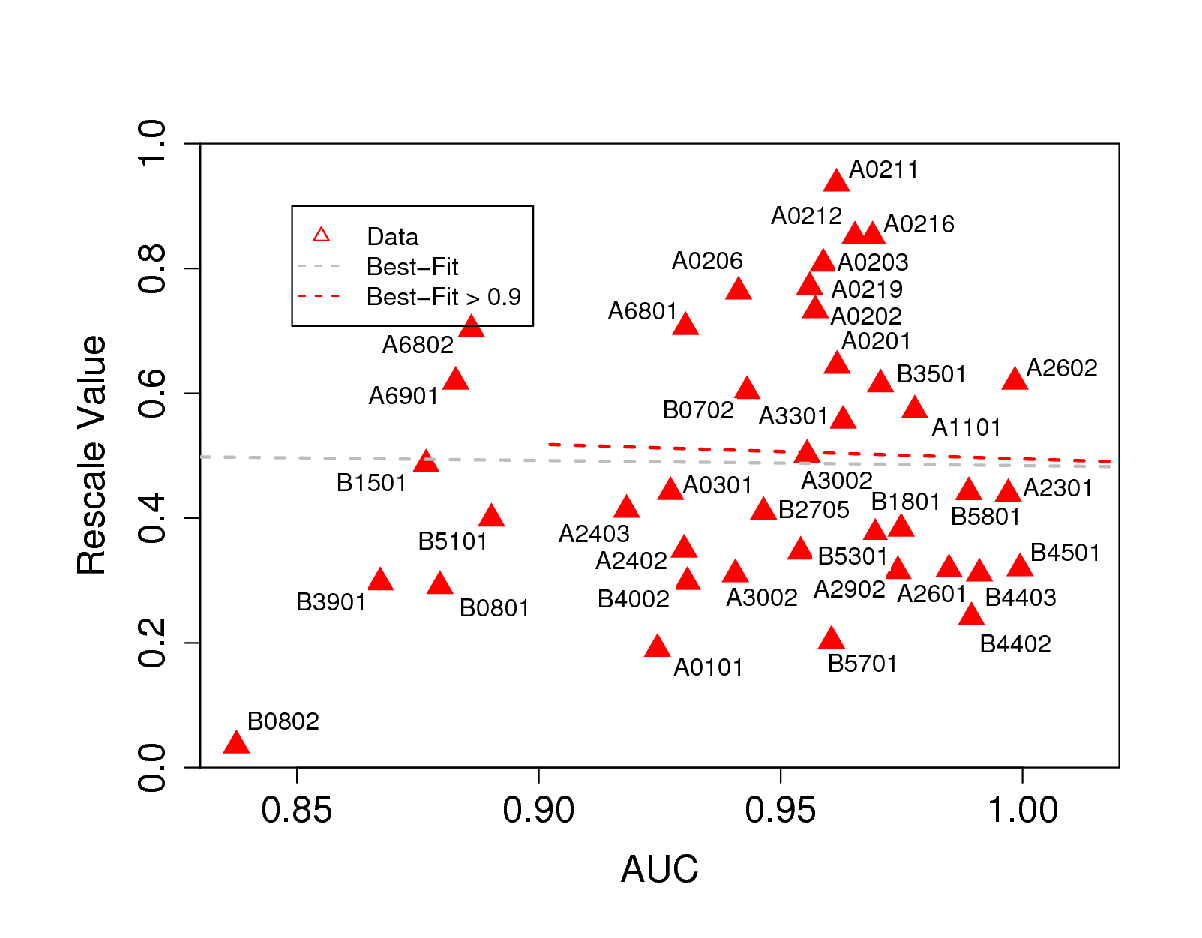
\includegraphics[width=14cm]{./Figures/chapter4/figure_2_edit_2}
%\rule{35em}{0.5pt}
\caption[The relationship between AUC and rescale value]{The relationship between AUC and rescale value. There is no evidence for a correlation of AUC and rescale value for the whole set of allele predictors ($R^2 = 0.0068$, $P = 0.606$), nor for the subset of predictors with an AUC $> 0.9$ ($R^2 = 0.0007$, $P = 0.887$). This analysis used the Lanl$^{661}$ epitope dataset.}
\label{chapter4/figure2}
\end{figure}

Consequently, it is unlikely that a correlation between rescale values and AUC values explains our findings. However, certain alleles like B0801 do have both a low rescale value and a low AUC. To double check that these poor accuracy predictors were not causing the inaccuracies in rescaled predictions we repeated our ROC curve analysis for Lanl$^{661}$ without the low accuracy predictors (those with an AUC value below 0.9; namely A6801, A6802, B3501, B0702, B0801, B0802 and B4501). In the remaining, reduced subset of predictors there was even less evidence for a correlation between AUC and rescale factor ($R^2 = 0.0007$, $P = 0.887$). For this subset of predictors the accuracy was still significantly better if rescaling was not applied (\fref{chapter4/reducedROC}; bootstrap test: $P < 0.001$) and comparable to the ROC curve analysis using the full set of alleles (\fref{chapter4/figure1} A).

Therefore, we believe there is no evidence to support the hypothesis that the reason rescaling is detrimental is because there is a correlation between rescale factors and AUC. 

\begin{figure}[htp]
\centering
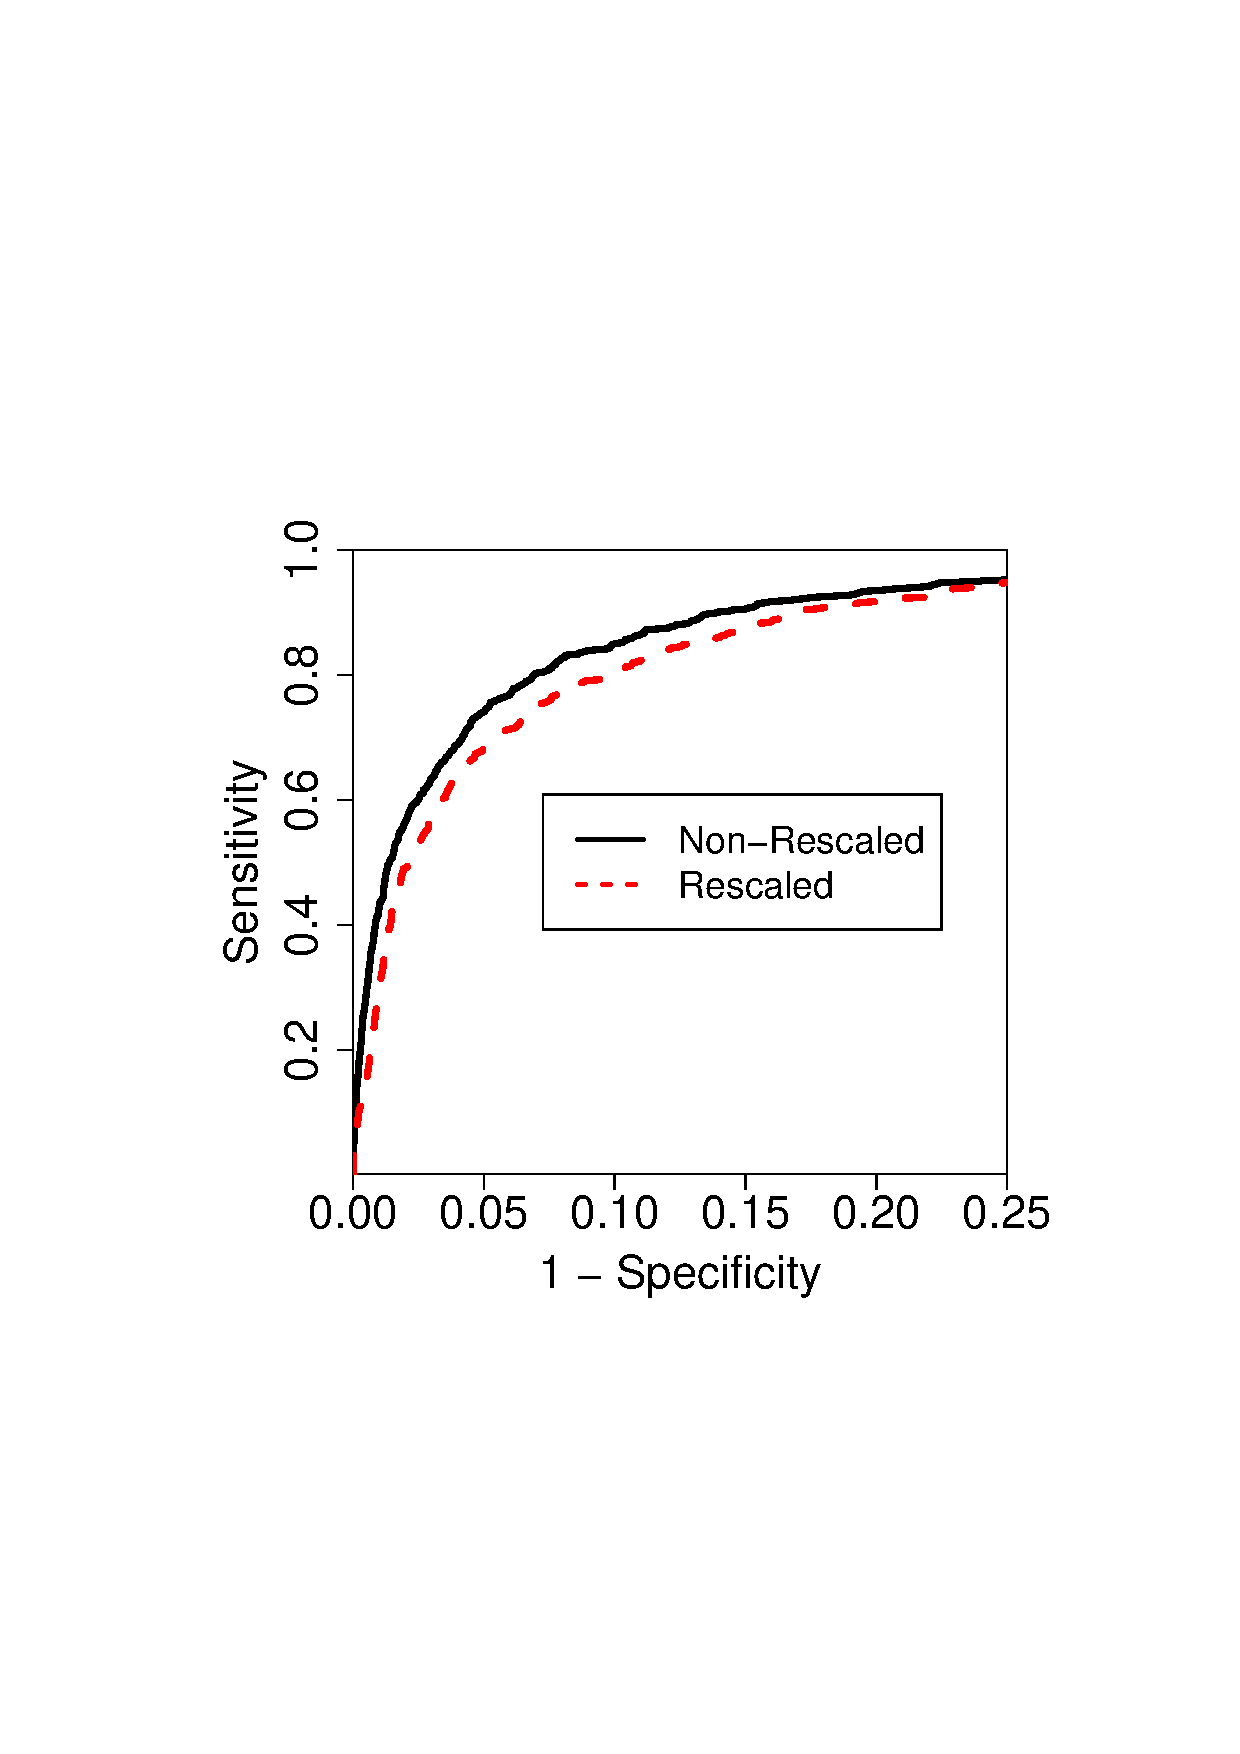
\includegraphics[width=10cm]{./Figures/chapter4/reducedROC}
%\rule{35em}{0.5pt}
\caption[The ROC curve analysis without low accuracy alleles]{The result of the ROC curve analysis, using the Lanl$^{661}$ dataset and excluding any alleles (7 in total) that had an AUC $< 0.9$ from \fref{chapter4/figureAffinityComp} (bootstrap: $P < 0.001$).}
\label{chapter4/reducedROC}
\end{figure}

\subsection{Other Measurements of Performance}

We used 3 other metrics \citep{larsen2007} to compare predictive performance with and without rescaling.

\begin{enumerate}
\item The rank of known epitopes was compared with non-epitopes from the same protein for both rescaled and non rescaled predictions. From \fref{chapter4/figureBoxplots}, it can be seen that the non-rescaled results produced significantly more accurate results for both epitope datasets (paired Wilcoxon ranked sum test, $P < 0.001$).

\begin{figure}[htp]
\centering
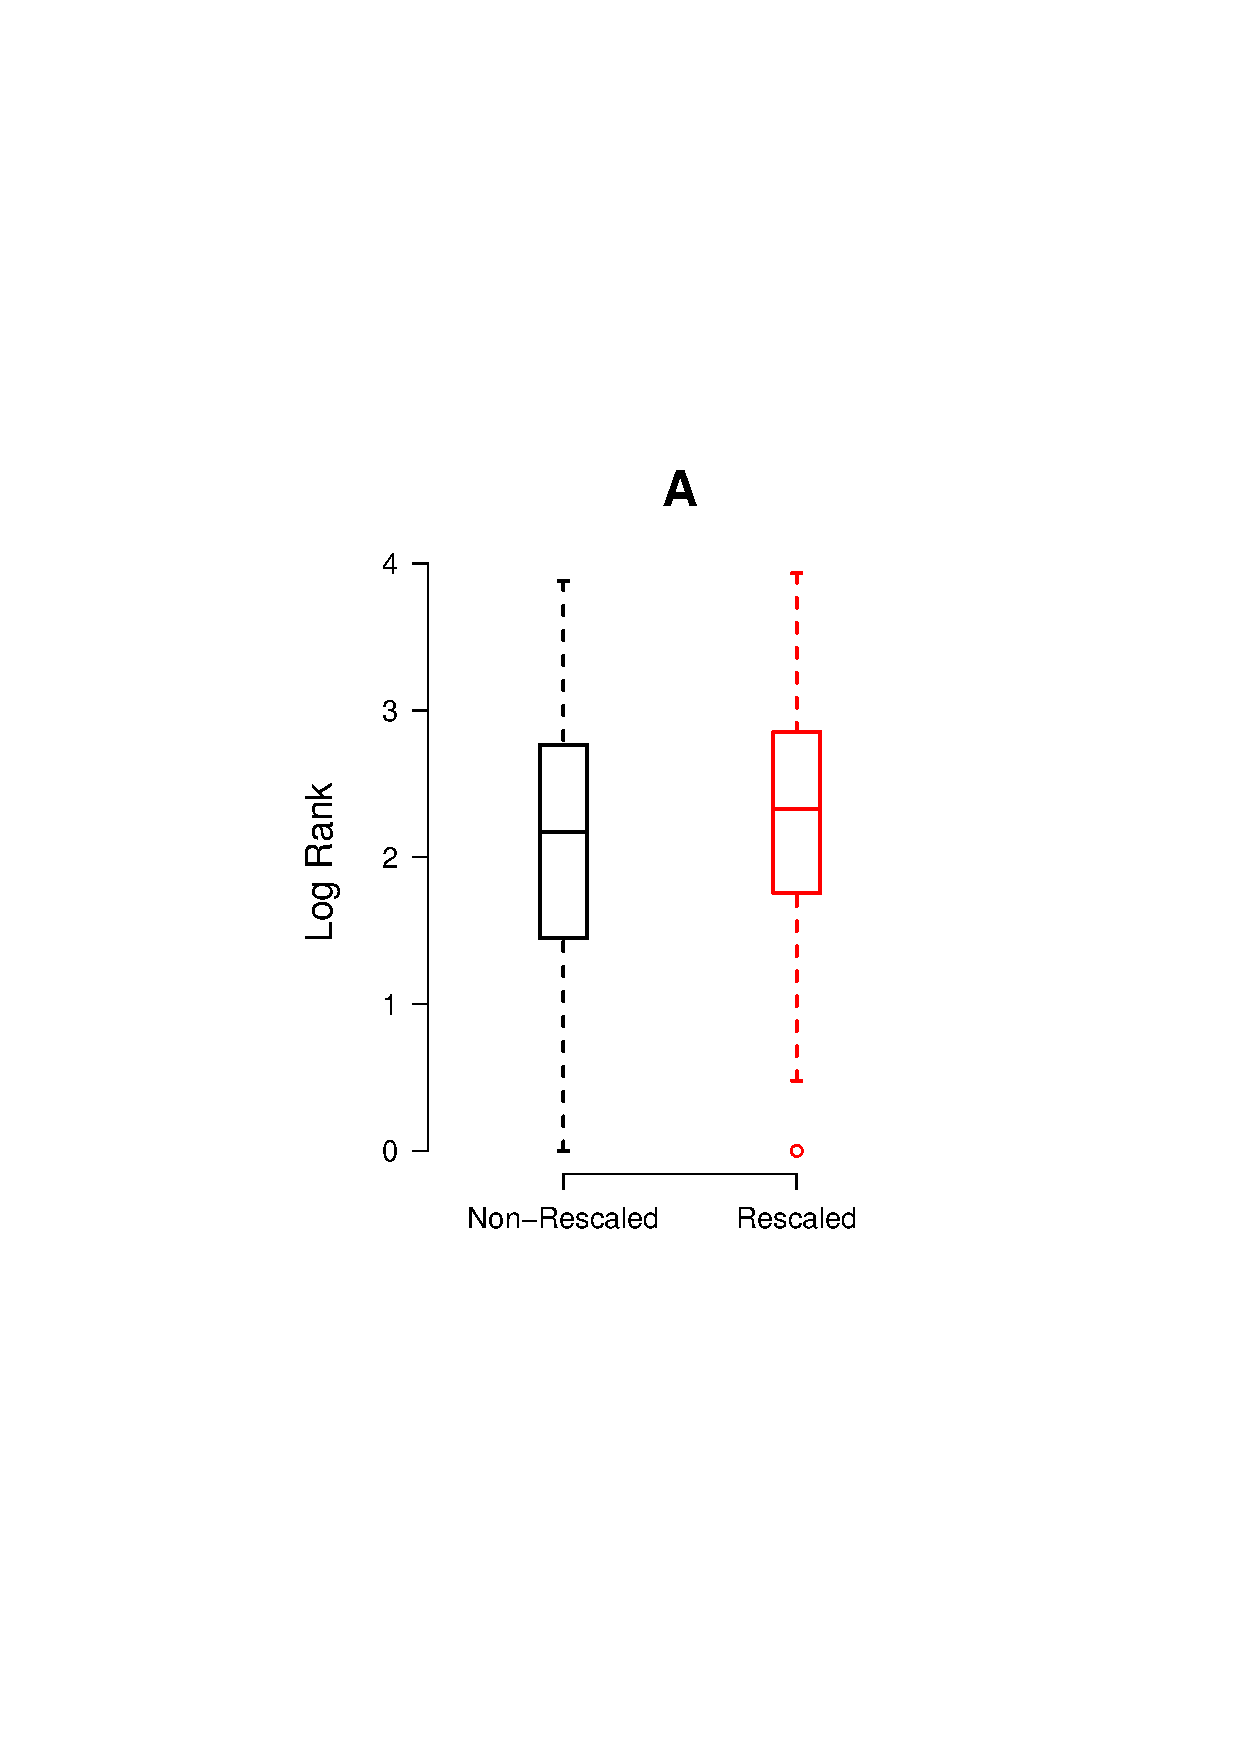
\includegraphics[width=7cm]{./Figures/chapter4/boxplotA}%
\hspace{0cm}%
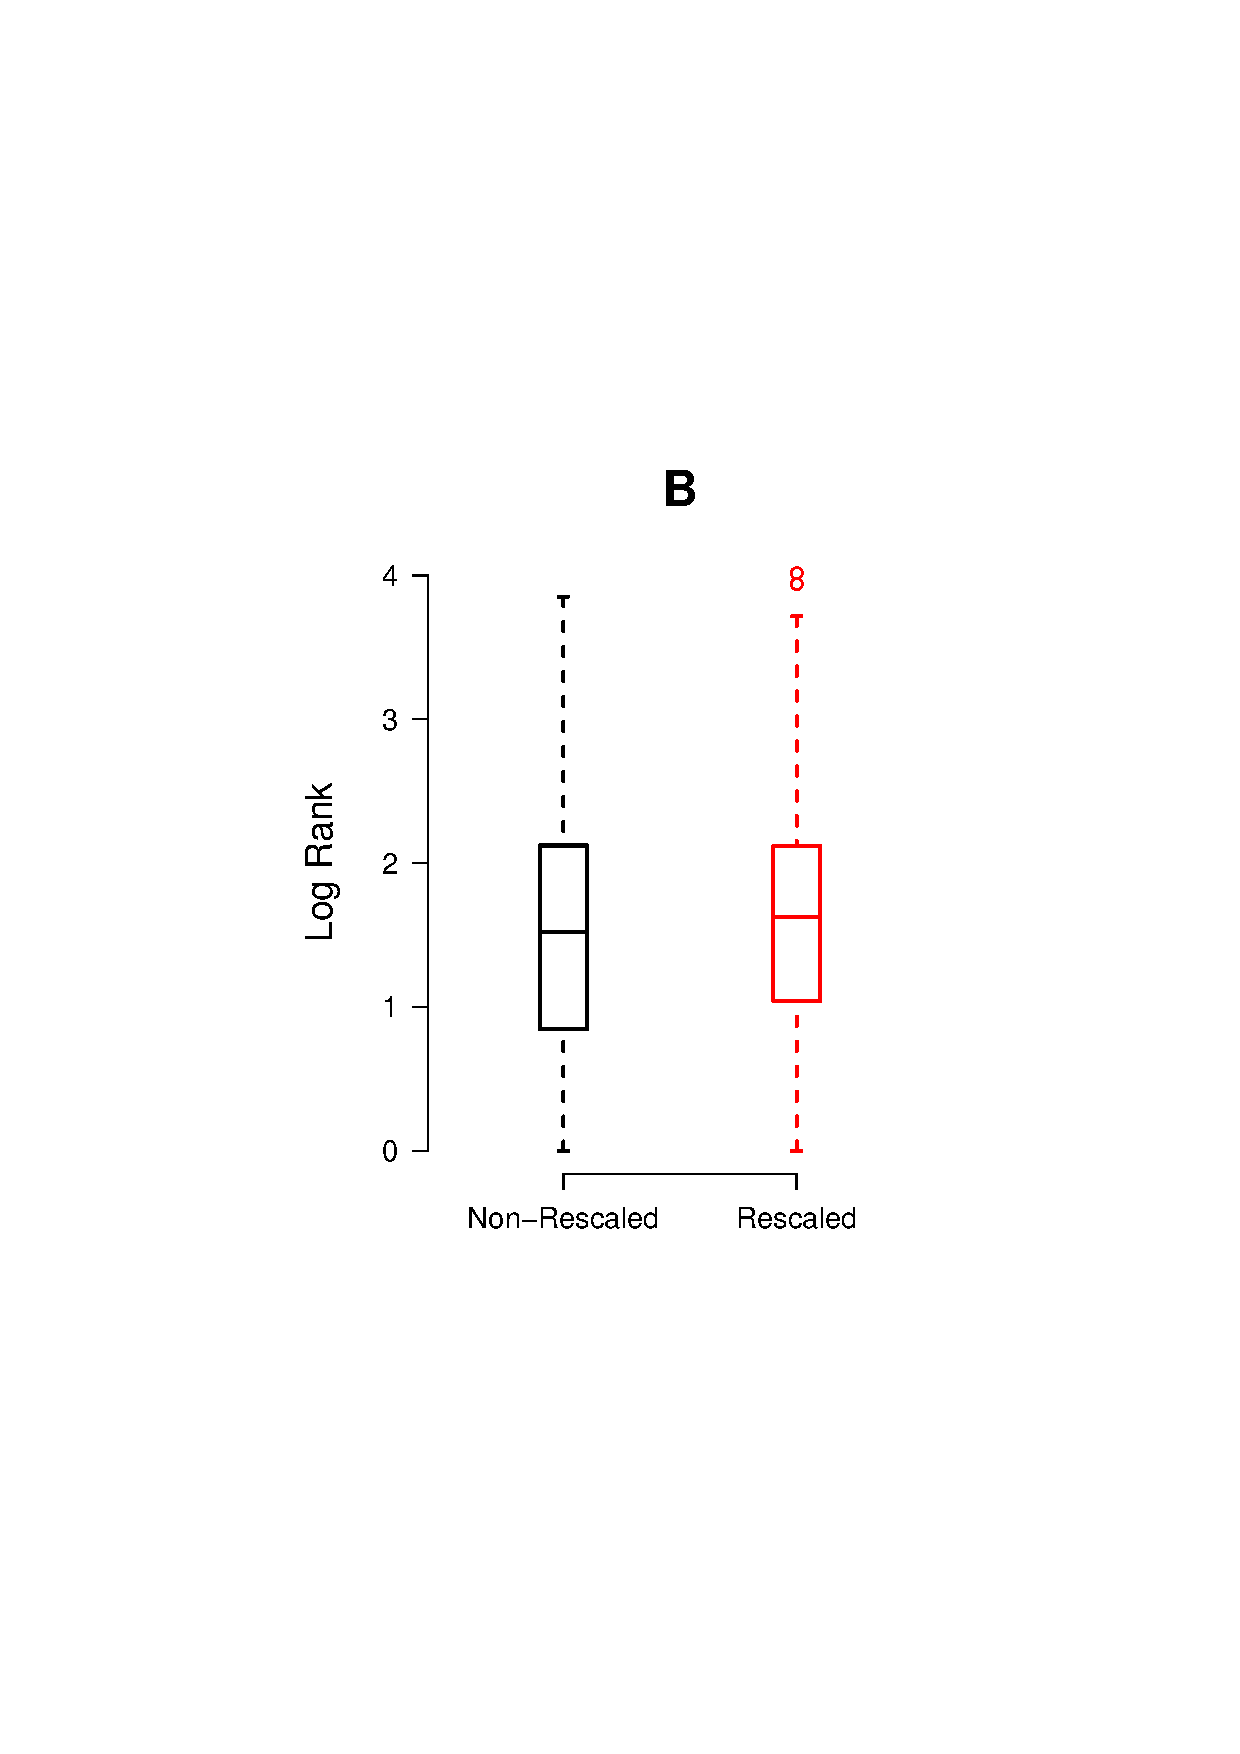
\includegraphics[width=7cm]{./Figures/chapter4/boxplotB} \\
\caption[]{\textbf{(A)} A box plot showing the summary statistics of the ranks ($\log_{10}$) of each of the 216 epitopes in the HIV dataset among all overlapping 9-mer in the epitopes' source proteins. The ranks of the epitopes were significantly lower for non-rescaled scores compared to rescaled scores (Paired Wilcoxon ranked sum test, $P < 0.001$). The non-rescaled scores produced a higher rank for 170 epitopes and rescaled scores for 24 epitopes. \textbf{(B)} The same analysis using 863 epitopes from the SYFPEITHI dataset. The ranks of the epitopes were significantly lower for non-rescaled scores compared to rescaled scores (Paired Wilcoxon ranked sum test, $P < 0.001$). The non-rescaled scores produced a higher rank for 474 epitopes and rescaled scores for 369 epitopes.}
\label{chapter4/figureBoxplots}
\end{figure}

\item Predicted binding affinities that had not been rescaled produced improved results compared to predictions that had been rescaled at given sensitivities using the epitope datasets from \citep{larsen2007} (\tref{chapter4/table2}).

\begin{table}[htp]
\begin{center}
\begin{tabular}{|c|c|c|c|}
\hline
Sensitivity & No Rescaling & Rescaling & Epitope Set \bigstrut \\
\hline
0.3 & 0.995 & 0.989 & \multirow{3}{*}{HIV$^{216}$} \bigstrut[t] \\
0.6 & 0.987 & 0.977 & \\ 
0.8 & 0.921 & 0.891 & \bigstrut[b] \\
\hline
0.3 & 0.998 & 0.997 & \multirow{3}{*}{SYF$^{863}$} \bigstrut[t] \\
0.6 & 0.991 & 0.991 & \\ 
0.8 & 0.974 & 0.973 & \bigstrut[b] \\ 
\hline
\end{tabular}
\end{center}
\caption[Specificity at specified sensitivity values]{The specificity of non-rescaled and rescaled results at specified sensitivity values. Epitope datasets are taken from \citep{larsen2007}.}\label{chapter4/table2}
\end{table}

\item Predicted binding affinities that had not been rescaled also showed an improvement over rescaled affinities when comparing the total number of true epitopes found among the top 5\% of peptides predicted to bind (\tref{chapter4/table3}), again using the epitope datasets from \citep{larsen2007}.

\begin{table}[htp]
\begin{center}
\begin{tabular}{|c|cc|}
\hline
Epitope Set & No Rescaling & Rescaling \bigstrut \\
\hline
SYF$^{863}$ & 0.885 & 0.877 \bigstrut[t] \\
HIV$^{216}$ & 0.718 & 0.690 \bigstrut[b] \\
\hline
\end{tabular}
\end{center}
\caption[The top 5\% of predicted binding affinities]{The fraction of the total number of epitopes in the 2 epitope datasets among the top 5\% of predicted binding affinities.}\label{chapter4/table3}
\end{table}

\end{enumerate}

\subsection{The Effect of Rescaling on Quantitative Predictions of Binding Affinities}
Using 2 sets of experimentally-derived epitope-allele binding affinities, we also showed that the correlation between predicted and experimental affinities was weaker with rescaling than without.

A set of 128 experimentally-derived epitope-allele binding affinities was extracted from the Immune Epitope Database and Analysis Resource \citep{peters2005}. This set of epitopes was known to have no involvement in the training of any of the allelic predictors in NetMHC v3.0 or NetCTL v1.2.

The relationship between the rescaled / non-rescaled predicted binding affinities and the experimental binding affinities was investigated (\fref{chapter4/figureAffinityComp}). Rescaling resulted in a significantly larger error (the difference between predicted and experimental affinity) compared to predicted binding affinities that were not rescaled ($P < 0.001$). Although rescaling would naturally result in a larger quantitative error, additionally, the correlation between predicted and experimental affinities was weaker with rescaling than without (rescaled: $P < 0.001$, Spearman's $\rho = 0.40$; not rescaled: $P < 0.001$, Spearman's $\rho = 0.51$).

The analysis was repeated using a second experimental dataset. This second dataset came from the Sette and Buus laboratories and included the experimental data used to train NetMHC and NetCTL. The results obtained using this second dataset were very similar to those obtained using the first, independent dataset (\fref{chapter4/figureCompareAll}).

\begin{figure}[htp]
\centering
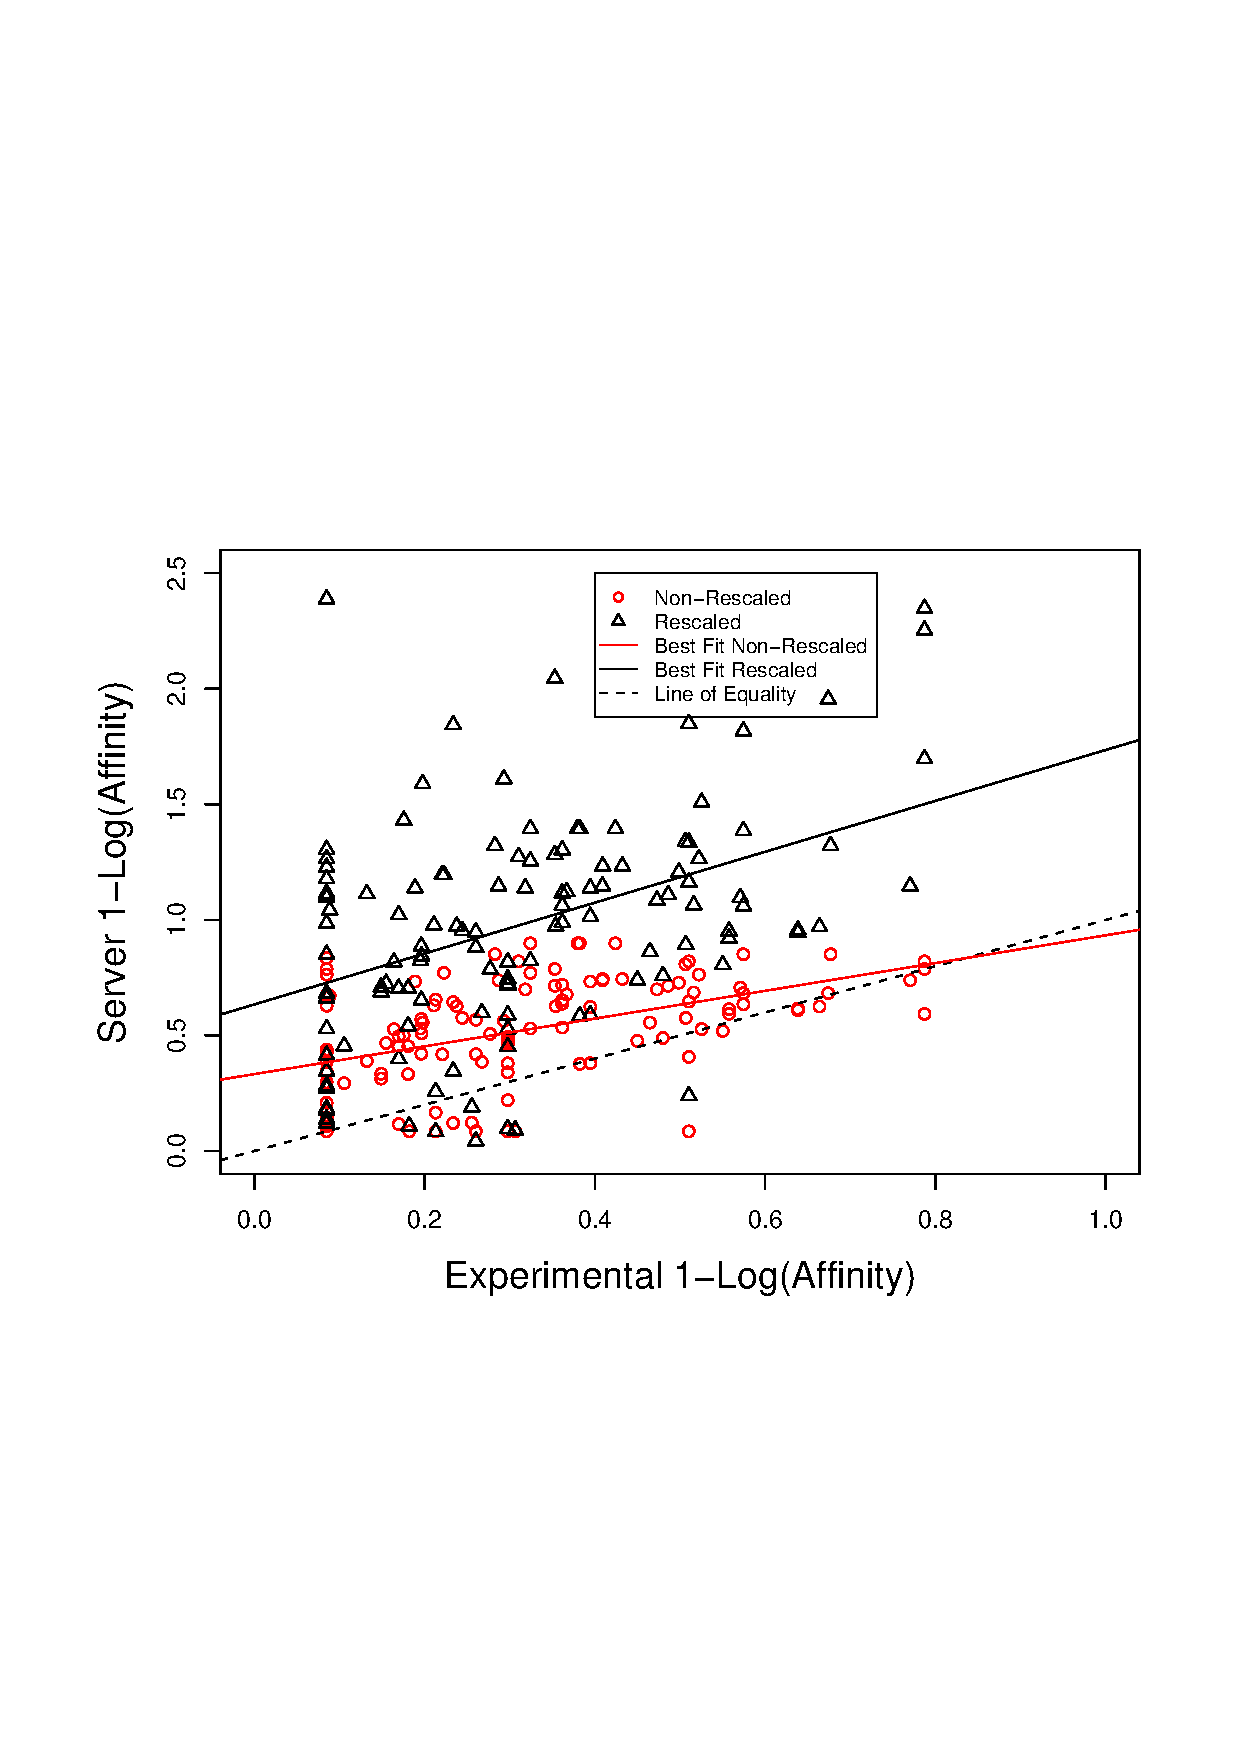
\includegraphics[width=14cm]{./Figures/chapter4/figureAffinityComp}
%\rule{35em}{0.5pt}
\caption[A comparison of experimental and predicted binding affinities]{The experimental binding affinities for 128 epitopes were obtained from IEDB \citep{peters2005} and converted to a log scale ($1-\log _{50000} \left( \text{affinity} \right)$). These epitopes were then tested using NetMHC v3.0 to produce 2 sets of predicted binding affinities; rescaled or non-rescaled. The predicted scores were also converted to a log scale ($1-\log _{50000} \left( \text{affinity} \right)$) and the non-parametric Spearman's $\rho$ was used to calculate the correlation between experimental and predicted data.}
\label{chapter4/figureAffinityComp}
\end{figure}

\begin{figure}[htp]
\centering
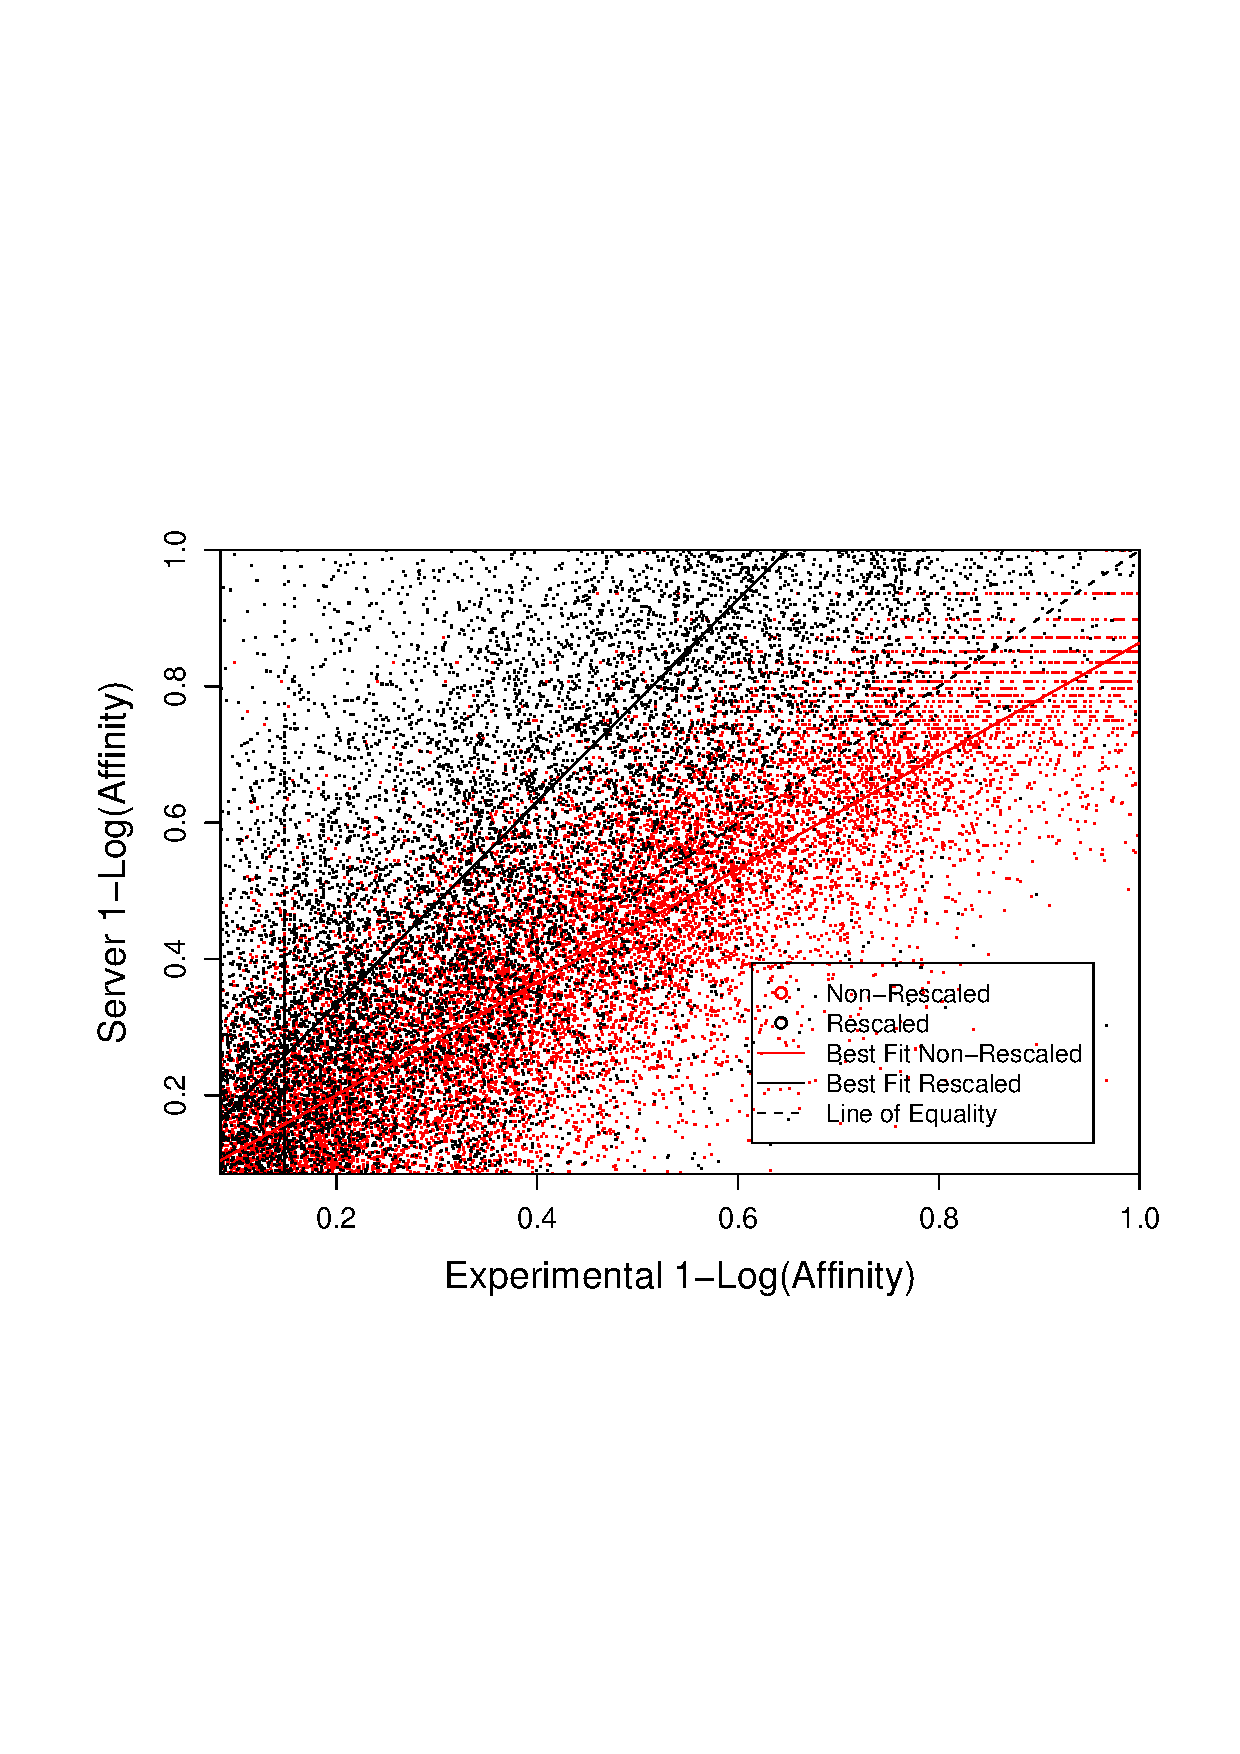
\includegraphics[width=14cm]{./Figures/chapter4/figureCompareAll}
%\rule{35em}{0.5pt}
\caption[A second comparison of experimental and predicted binding affinities]{The experimental binding affinities for 29,336 epitopes were obtained from IEDB and converted to a log scale ($1-\log _{50000} \left( \text{affinity} \right)$). These epitopes were then tested using NetMHC v3.0 to produce 2 sets of predicted binding affinities; rescaled or non-rescaled. The predicted scores were also converted to a log scale ($1-\log _{50000} \left( \text{affinity} \right)$) and the non-parametric Spearman's $\rho$ was used to calculate the correlation between experimental and predicted data. The correlation between non-rescaled predicted affinities and experimental data showed a $P$ value of $< 0.001$ (Spearman's $\rho$ = 0.877). Rescaled predicted affinities and experimental data gave a $P$ value of $< 0.001$ (Spearman�s $\rho$ = 0.816). The absolute difference between the 2 best-fit lines and the line of equality was calculated and it was shown that the non-rescaled values were significantly closer to the line of equality (Wilcoxon Paired Signed Rank Test; $P$ value $< 0.001$).}
\label{chapter4/figureCompareAll}
\end{figure}

\subsection{The Effect of Negative Data Volume}\label{chapter4/results/NegVol}

As explained in \sref{chapter4/methodsDatasets}, we multiplied the negative set of each dataset by the number of allele predictors being tested. This was to mirror an analysis where one would check every possible peptide-allele pair of a pathogen-MHC class I interaction when searching for potential epitopes. A possible argument was that the resultant positive/negative ratio in our datasets was unrealistically low with such a high proportion of negative data. To counter this, the SYF$^1$ dataset was modified to contain 148 positive epitopes and 78,111 negative peptides, which gave a positive/negative ratio of 0.2\%, a figure close to the estimated 1\% of all natural peptides that would bind to a given MHC molecule \citep{larsen2005}. In order to test the difference in prediction accuracy between rescaled and non-rescaled predicted affinities with this reduced dataset, each of the 78,111 negative peptides was randomly paired with 1 of the 10 supertype predictors (see \sref{chapter4/methodsSYF1}) and the predicted binding affinity was found for each of theses pairs. Rescaling again resulted in a significant loss of performance (bootstrap test: $P < 0.001$, \fref{chapter4/figureReducedNeg}).

Related to this result, we performed a general analysis of the effect of positive and negative set size on the AUC values obtained in ROC curve analysis. As this is outside the scope of this chapter, this is explained in \aref{AppendixA/sizeEffects}.

\begin{figure}[htp]
\centering
\includegraphics[width=12cm]{./Figures/chapter4/figureReducedNegative}
\caption[The effect of a reduced negative dataset]{The result of the ROC curve analysis, using the SYF$^1$ dataset, with a negative set of 78,111 peptides. The difference remains significant between the two curves (bootstrap test: $P < 0.001$).}
\label{chapter4/figureReducedNeg}
\end{figure}

\subsection{Is Rescaling Necessary to Maintain Low Variation in Sensitivity?}

Another argument that could be made for rescaling is that, in its absence, those allele predictors with a lower accuracy would have lower sensitivity i.e.~fewer epitopes would be detected from those particular alleles (Morten Nielsen, pers.~comm.). We tested this hypothesis using the SYF$^1$ dataset. A score threshold value for rescaled and non-rescaled affinity values was identified at a specificity of 0.95 for the complete dataset (0.2068 for non-rescaled affinity values and 0.4330 for rescaled affinity values, using $1-\log _{50000} \left( \text{affinity} \right)$). Next the sensitivity and specificity values per supertype allele were calculated at these threshold values. The result is shown in \fref{chapter4/figureRevArg}. There is no evidence for a large decrease in the variation in allelic sensitivity upon rescaling. The ranges of sensitivities are identical with or without rescaling and the standard deviations are very similar (0.1526 non-rescaled, 0.1528 rescaled), if anything, slightly higher upon rescaling.

\begin{figure}[htp]
\centering
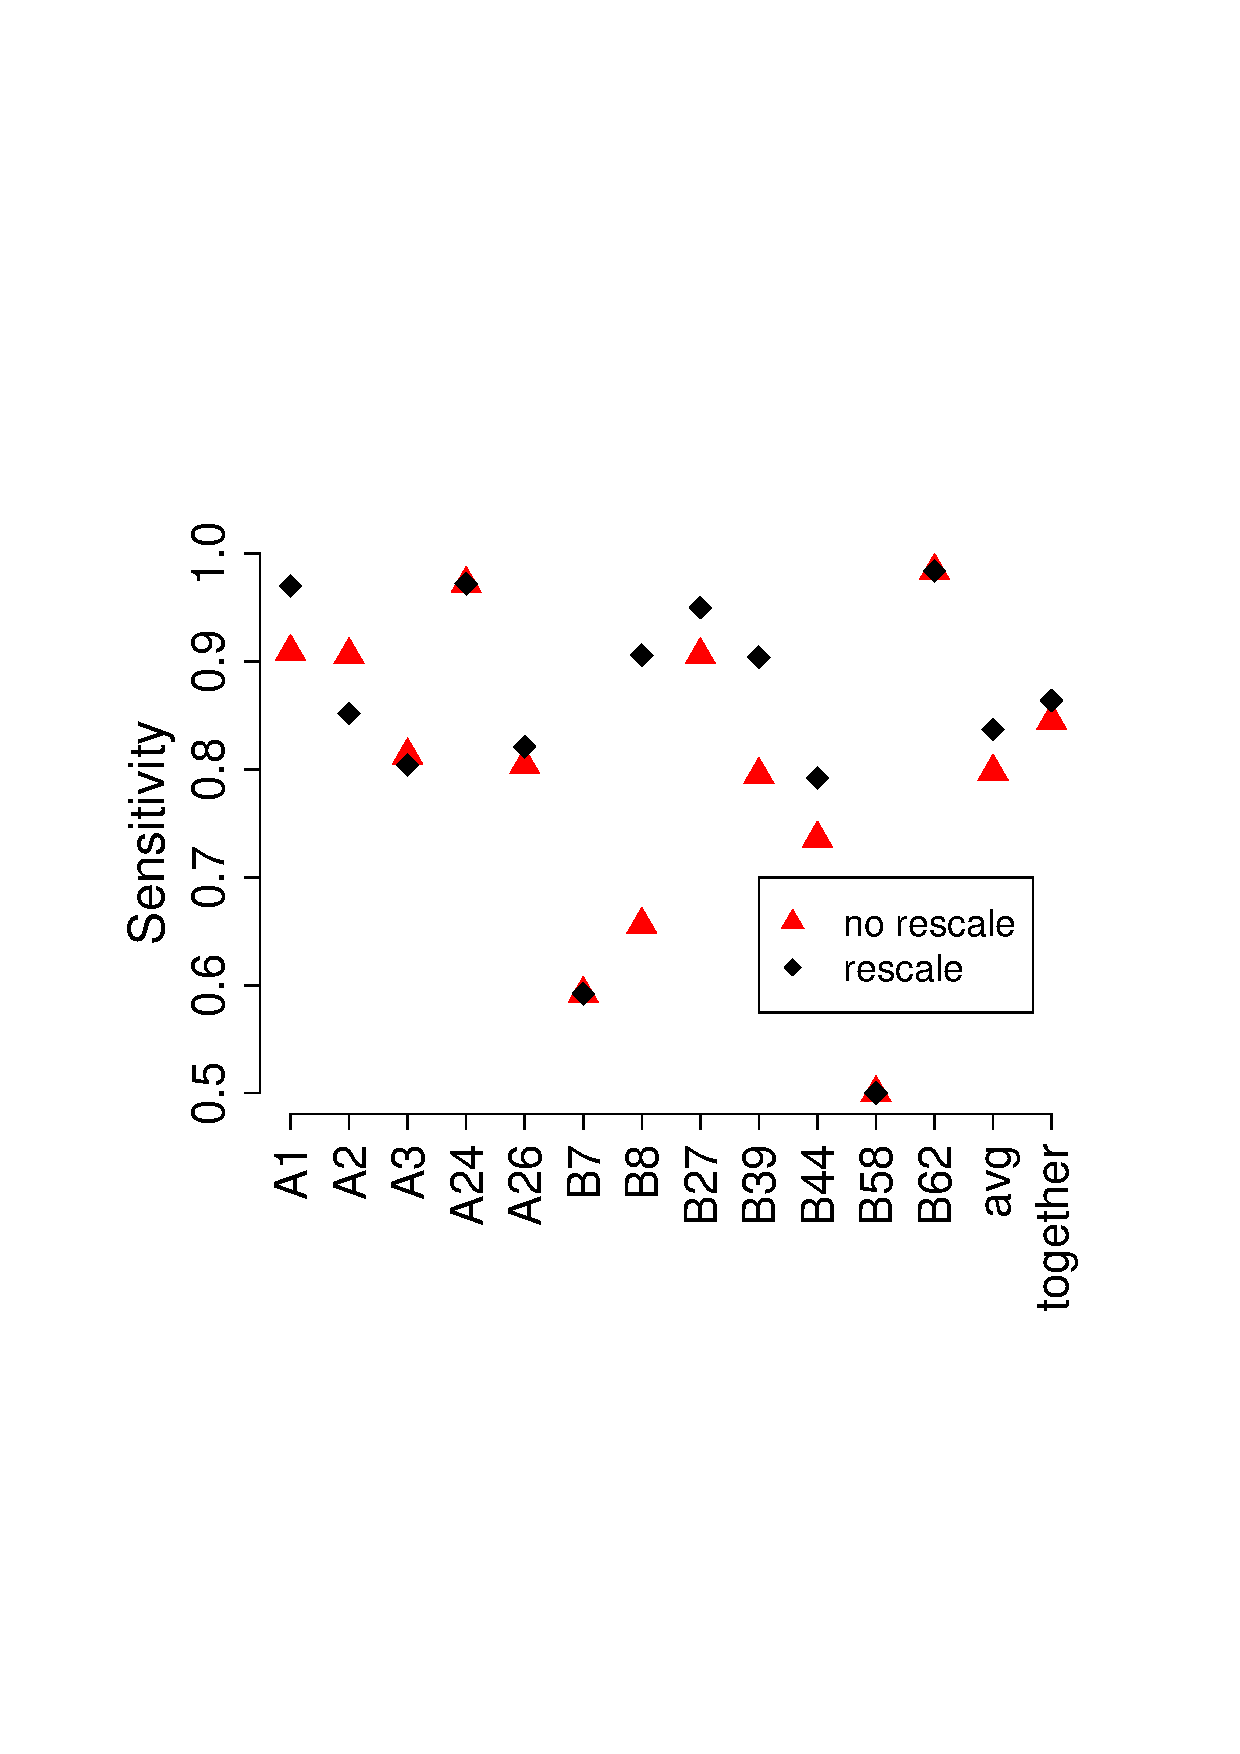
\includegraphics[width=12cm]{./Figures/chapter4/figureRevArg}
\caption[The effect of rescaling on sensitivity]{The effect of rescaling on sensitivity. For each supertype, the sensitivity was calculated when rescaling and not rescaling the predicted binding affinities. The final two results give the average sensitivities across all supertypes (`avg') and the sensitivities of all supertypes measured together (`together').}
\label{chapter4/figureRevArg}
\end{figure}

%%%%%%%%%%%%%%%%%%%%%%%%%%%%%%%%%%%%%%%%%%%%%%%%%%%%%%%%%%%%%%%%%%%%%%%%%%%%%%%%%%%%%%%%%%%%%%%%%%%%

\section{Producing Metaserver}\label{chapter4/results/metaserver}

These results demonstrated a significant improvement in accuracy over NetMHC v3.0 and NetCTL v2.1 when classifying epitopes across a number of HLA class I alleles. Therefor, we decided to produce our own web-based prediction server based on these results, which we called Metaserver.

Metaserver is summarised in \eref{chapter4/equation1}. In this calculation the NetMHC estimated binding affinity is still combined with a rescale value in order to take advantage of the NetCTL-specific information relating to the processing (TAP and cleavage) of the peptide before it binds to HLA class I. However, the rescale value for Metaserver is the same across all alleles and is an average of the rescale values for each individual allele. In summary, Metaserver takes binding information from NetMHC, TAP and cleavage information from NetCTL, but removes the assumption that each HLA class I binds the same number of peptides by `averaging out' the rescaling of the predicted binding affinity. 

\begin{align}
\text{Metaserver Epitope Score} =& \text{ NetMHC Binding Affinity} / \text{~`Averaged' Rescale Value } + \nonumber \\
& \; w_{1} * \text{NetCTL TAP} + w_{2} * \text{NetCTL Cleavage}
\label{chapter4/equation1}
\end{align}

\noindent
$w_1$ and $w_2$ above represent the weightings that are applied to the TAP and cleavage prediction scores respectively. In all calculations, $w_1 = 0.05$ and $w_2 = 0.15$. Metaserver uses a Perl LWP script to access the web servers NetMHC and NetCTL and the website itself is written in PHP (\fref{chapter4/websiteView}). 

\begin{figure}[htp]
\centering
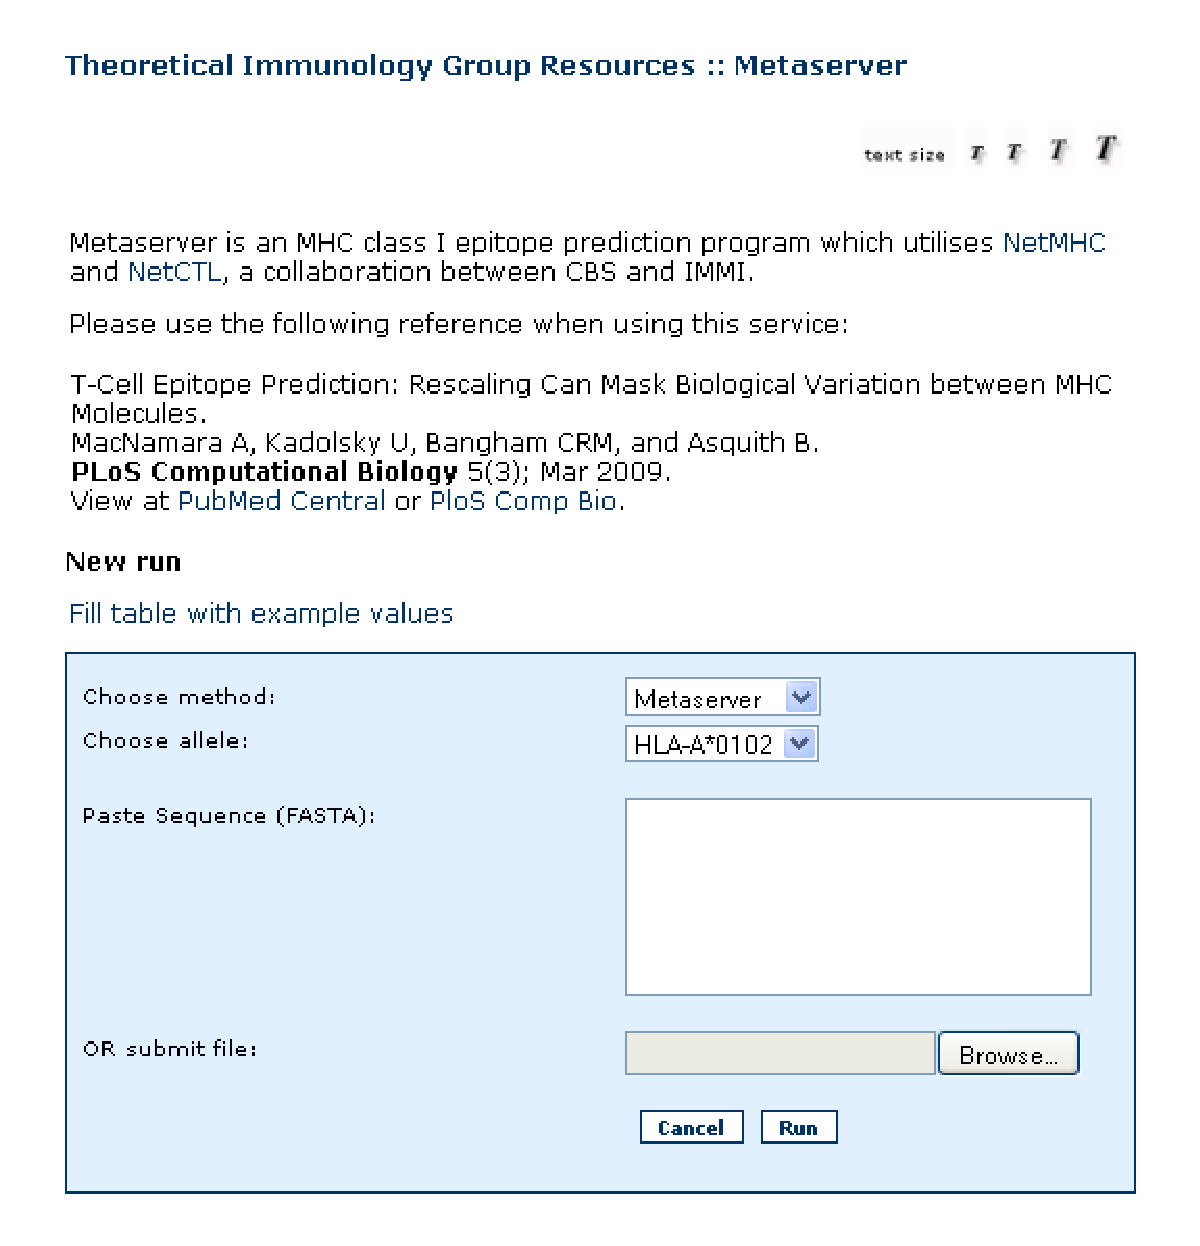
\includegraphics[width=10cm]{./Figures/chapter4/websiteView}
%\rule{35em}{0.5pt}
\caption[The Metaserver website]{A screenshot showing the Metaserver web-based resource. The site is hosted at:\\ \href{http://linuxwebdev.cc.ic.ac.uk/theoreticalimmunology/trans/metaserver.php}{\texttt{http://linuxwebdev.cc.ic.ac.uk/theoreticalimmunology/trans/metaserver.php}}\\}
\label{chapter4/websiteView}
\end{figure}

%%%%%%%%%%%%%%%%%%%%%%%%%%%%%%%%%%%%%%%%%%%%%%%%%%%%%%%%%%%%%%%%%%%%%%%%%%%%%%%%%%%%%%%%%%%%%%%%%%%%

\section{Discussion}

Rescaling is, in theory, a sound approach to improving epitope prediction and in particular comparability of predictions obtained using different allelic predictors. However, using a number of different measures of accuracy, in the context of two commonly used prediction methods, we have demonstrated that rescaling actually impairs rather than improves predictive performance and comparability. We suggest that rescaling predicted affinities results in a loss of information that outweighs any advantage gained in correcting for differences in training data. 

The first approach used ROC curve analysis and showed clear differences between rescaling and non-rescaling. The ROC curve gives a graphical representation of how well the prediction method ranks true epitopes among a set of non-binding peptides. Or to use an analogy, how efficient it is at finding the epitopic needle in a haystack of random peptides. From \fref{chapter4/figure1}, it is clear that rescaling across all allelic predictors results in a performance loss in terms of how well the method ranks its peptides by binding affinity; that is, rescaling impairs intra-allelic comparisons. This loss could be demonstrated using epitope data from a number of sources (SYFPEITHI, the HIV Molecular Immunology Database) and with two different methods of prediction (the combined approach of NetCTL v1.2 and NetMHC v3.0). This effect of rescaling would be detrimental to any studies screening across a number of alleles for possible epitopes (such as \citep{wang2007}). The effect of this performance difference can be gauged from \fref{chapter4/figure1} A. In order to identify correctly 85\% of the epitopes the percentage of false positives detected was 9\% and 15\%, for non-rescaled and rescaled methods respectively. To put this result into context, the viral protein NS1 from the H5N1 strain of Avian Influenza A consists of 221 overlapping nonamers. To screen this protein for potential epitopes, 33 epitopes would need to be experimentally checked for each MHC molecule of interest if rescaled predictions were used, as opposed to 20 for the non-rescaled predictions (providing 85\% epitope coverage was sufficient).

Added to the significant results from the ROC curve analysis, we also demonstrated the positive effect of removing rescaling in terms of the correlation with experimental data (\fref{chapter4/figureAffinityComp}) and also in terms of per-protein and sensitivity analysis (\fref{chapter4/figureBoxplots} and \tref{chapter4/table2} and \tref{chapter4/table3}). Taken together, these results strongly demonstrate the improvement in accuracy of removing the condition of rescaling when comparing predictions between alleles.

There has been little research on the variation in `stickiness' among MHC molecules, i.e.~whether some MHC class I molecules are capable of binding to a greater number of epitopes than others. The binding motifs for MHC-peptide binding vary across the range of alleles, but the assumption made for rescaling is that each molecule would bind to the same number of peptides out of a large random selection. Estimates based upon mass spectrometry suggest that over 2,000 peptides are associated with HLA-A2.1 and -B7 and it is speculated that the actual total could be over 10,000 per MHC molecule \citep{Engelhard1994a}. However, it is not known how this number varies between molecules. It has been postulated that the twin constraints of effective pathogen recognition but tolerance of self would result in a very narrow range of promiscuity for viable MHC class I molecules \citep{George2005}. Contrary to this, recent research has shown that this range may be wider than initially envisaged \citep{Frahm2007} and our results suggest that there is considerable inter-allelic variation in promiscuity.

This data may also be informative regarding optimization of peptide cargo in the endoplasmic reticulum (ER). We would argue that peptide optimization is the biological interpretation of rescaling: alleles have similar numbers of epitopes because peptides with a lower binding affinity are replaced in the ER\@. We know that optimisation cannot be complete because otherwise every allele would just present one epitope: the one with highest affinity. However, it seems likely that there is a degree of optimization \citep{Elliott2006, Williams2002}. The observation that rescaling gives worse predictions may put a bound on how much optimisation is occurring. Allied to this, it has been observed that the release of an MHC class I molecule from the peptide-loading complex with a suboptimal peptide takes precedence over the prolonged detention of the MHC class I molecule in the complex until an optimal peptide comes along \citep{Elliott2006}. Hence, peptide optimization acts to reduce inter-allelic variation and promiscuity results from inter-allelic variation in allele-peptide affinity. However, this peptide optimization is limited by time and is not complete and hence, we note this variation in promiscuity across different alleles.

In summary, we suggest that much of the observed variation between allelic predictors reflects genuine biological information which should not be discarded as experimental noise and that rescaling is based on an unjustified assumption: that all alleles bind the same number of peptides. Removing this assumption, we have demonstrated a significantly improved predictive performance. These conclusions are important both for studies that use prediction methods to understand the CTL response and for T cell epitope discovery programs where avoiding rescaling could save a large amount of experimental effort, ultimately leading to improved vaccine implementation.

In the context of our work on HTLV-I, this research allowed us to fully test NetMHC v3.0 as software to predict HTLV-I epitopes. NetMHC v3.0 demonstrated high accuracy identifying experimentally verified epitopes from HIV (Lanl$^{179}$ and Lanl$^{661}$), human and other viral sources (SYF$^1$). \cref{Chapter6} follows on from this verificiation to test NetMHC v3.0 in the context of HTLV-I and and hence predict HTLV-I epitopes. From this information, we could test hypotheses relating to protective and detrimental effects of MHC class I alleles. 
	% Rescaling
% Chapter 5, changed from chapter 6 - still labelled as chapter 6

\chapter{The Prediction of Disease From Peptide Binding Affinities}
\label{Chapter6}
\lhead{Chapter 5. \emph{The Prediction of Disease From Peptide Binding Affinities}}

\section{Introduction}

The application of epitope prediction software has almost exclusively been used to identify specific epitope - MHC class I complexes i.e.~identifying epitopes from a predefined protein that bind to a particular MHC class I molecule \citep{Westrop2009a}. To the best of our knowledge, this study was the first to use this software to define the epitope repertoire of a virus (HTLV-I) across a large cohort of individuals, in order to identify the epitope properties of a successful CD8$^+$ T cell response. The possibility of success depended on the accuracy of the epitope prediction software used. In \cref{Chapter4}, we tested this software and produced our own implementation (Metaserver) of two widely available web-based epitope prediction servers, NetMHC and NetCTL. We showed that Metaserver was able to predict HIV epitopes with high sensitivity (\sref{chapter4/results}). These results allowed us to bring forward this software to use with HTLV-I and test our hypotheses concerning the role of HLA class I in infection.

Most HTLV-I-infected individuals have a strong, chronically activated CD8$^+$ T cell response to HTLV-I and it is unclear why this fails to eradicate the virus. Furthermore, there is evidence for both protective effects \citep{Jeffery1999, Vine2004, Asquith2005a} and pathogenic effects \citep{Jacobson1990, Greten1998, Kubota2000, Jacobson2002} of HTLV-I specific CD8$^+$ T cells. As in all viral infections, the attributes of a protective antiviral response \emph{in vivo} are unknown, although specificity for the viral protein Tax is a strong candidate. There are good reasons to believe that a Tax-specific CD8$^+$ response \citep{Sundaram2003} may be particularly protective. Firstly, Tax is the immunodominant HTLV-I antigen in this response \citep{Kannagi1991, Goon2004}. Secondly, HLA-A*02, which is associated with protection in southern Japan \citep{Jeffery1999}, binds several Tax epitopes \citep{Parker1994}, notably Tax 11--19, which is bound unusually strongly \citep{Hausmann1999}. Thirdly, Tax is one of the first HTLV-I proteins to be expressed and it has been shown, for HIV-I infected cells \emph{in vitro}, that CD8$^+$ T cells specific to early viral proteins are particularly effective in viral control \citep{Baalen2002a}. Finally, it has been shown that the selective pressure exerted on Tax is higher in asymptomatic carriers than in those that have developed HAM/TSP \citep{Niewiesk1994}. 

\subsection{How can CD8$^+$ cell protective efficacy be quantified?}

Measurements of CD8$^+$ cell frequency, phenotype, function and specificity are informative but, because antigen load influences each of these factors, it can be difficult to ascertain if a particular immune profile is the cause or effect of good pathogen control \citep{Barber2006, Lichterfeld2007a, Streeck2008, Bangham2009}. An alternative approach is host genotype analysis. Polymorphisms in immune-related genes, particularly the HLA class I genes, have been associated with outcome in \emph{Plasmodium falciparum}, \emph{Mycobacterium tuberculosis}, HIV-I, HTLV-I and Hepatitis B Virus infection. The benefit of a genotypic analysis is that the direction of causality is unequivocal; the drawback is that, in common with all `omics' approaches to identify biomarkers, mechanistic insight is limited. Provided linkage disequilibrium can be ruled out, class I associations imply that the protective effect is mediated by CD8$^+$ T or NK cells. However, why one particular allele should be protective remains unclear and so provides no information about how to manipulate the immune response to enhance protection.

Hence, the aim of this section was to develop a method to test the hypothesis that the effectiveness of an individual�s HTLV-I-specific response and thus their proviral load and HAM/TSP risk was determined by the epitope binding properties of their HLA class I alleles. Specifically, we focused on the question, ``does strong binding to peptides from a specific HTLV-I protein benefit the host?''. We used a novel ranking measure to define the relationship between HLA class I and HTLV-I proteins. This approach is generally applicable to all pathogens, including those in which few epitopes have been identified experimentally.

\section{Methods}

\subsection{Epitope Prediction}\label{chapter5/MethPred}

We used two different algorithms to predict HLA class I epitopes: Metaserver and Epipred. Figures based on Metaserver predictions are in the main text, the corresponding figures for Epipred are in supplementary information.

\subsubsection{Metaserver}

Metaserver is described in detail in \sref{chapter4/results/metaserver}. Briefly, it is a combination of two web-based prediction methods that use artificial neural nets, NetCTL v1.2 \citep{larsen2005} and NetMHC v3.0 \citep{buus2003, nielsen2003}. Metaserver combines the two methods and removes a normalising assumption (which maintains that all alleles bind the same number of peptides) to produce a technique that shows improved accuracy in epitope prediction \citep{Macnamara2009} and predicts epitopes for 43 HLA molecules.

%Metaserver is a combination of two web-based prediction methods that use artificial neural nets, NetCTL v1.2 \citep{larsen2005} and NetMHC v3.0 \citep{buus2003, nielsen2003}. NetCTL is an integrated method that predicts TAP transport, proteasomal cleavage and HLA binding for 12 different class I alleles. NetMHC v3.0 predicts HLA-peptide binding for 43 HLA molecules. Metaserver combines the two methods and removes a normalising assumption (which held that all alleles bind the same number of peptides) to produce a technique that shows improved accuracy in epitope prediction \citep{Macnamara2009} (and chapter *** REF ***) and predicts epitopes for 43 HLA molecules.

\subsubsection{Epipred}

In order to validate our results, we used a second, independent method of epitope prediction \citep{heckerman2007}. Epipred uses a logistic regression model that is trained on all available data across all HLA class I alleles and then specified for an individual allele. 

\subsection{Epitope Prediction - Allele Coverage}\label{AlleleCoverage}

Metaserver provided coverage of 84\% of the total count of A/B alleles in the Kagoshima cohort. 

The missing alleles are: A0207, A0210, A2603, A3201, B1301, B1501, B1508, B1511, B1518, B2704, B3701, B3802, B4005, B4006, B4601, B4801, B5201, B5501, B5504, B5601, B5603, B5605, B5705, B5901, and B6701. 

We were able to obtain predictions for \{A0207, A0210\}, A2603 and \{B4005, B4006\} to a resolution of 2 digits by combining the predictions of other A02*, A26* and B40* predictors according to their frequency in Kagoshima. For example, to obtain a 2-digit ``A02'' predictor that could be used in place of A0207, \eref{chapter6/equation1} was used:

\begin{equation}
\mbox{A02 Binding Affinity} = \frac{\sum_{i = 3^{rd}/4^{th} digit}^n\left(\mbox{Binding Affinity: A02i} * \mbox{Freq A02i}\right)}{\sum_{i = 3^{rd}/4^{th} digit}^n \mbox{Freq A02i}}
\label{chapter6/equation1}
\end{equation}

A02i being the set of $n$ 4-digit A02 alleles in the Kagoshima cohort for which we have predictors.

\subsection{Prediction Quality}

The accuracy of epitope prediction algorithms has increased to such an extent that the correlation between predicted binding affinities and measured binding affinity is as strong as the correlations of measurements between different laboratories \citep{Peters2006}. The specificity of epitope predictors has been tested by predicting a set of CTL epitopes and subsequently verifying CD8$^+$ T cell responses against these epitopes experimentally. Using this technique has yielded true-positive (correctly predicted) estimates of 62-80\% \citep{Schmid2008}. Using the more direct approach of mass spectrometry to determine HLA-peptide binding yielded a true positive rate of greater than 98\% \citep{Fortier2008}. Additionally, we verified the prediction software we used (Metaserver and Epipred) for HTLV-I peptides (\sref{chapter6/methods/verify}).

\subsection{The Rank Measure}\label{RankMeasure}

Both prediction methods that we use produce a score for each peptide-HLA that represents the binding strength of that complex. In theory this score would allow us to compare predicted binding affinities between alleles. However, between allele comparisons can be problematic. Firstly, within-allele comparisons (i.e.~predictions for different peptides to the same allele) are thought to be more comparable than predictions between alleles \citep{larsen2005}. Secondly, whether or not a normalisation procedure should be applied for between-allele comparisons is still being debated in the community \citep{Macnamara2009}. To avoid the potential problem of between-allele comparisons we used the rank measure technique introduced by Borghans \emph{et al.} \citep{borghans2007} in which she quantified the strength of peptide-HLA class I binding for peptides from a particular protein by ranking the strength of binding of peptides from the protein of interest to the allele amongst the strength of binding of peptides from the entire proteome to that allele. Specifically, we split each protein in the HTLV-I reference sequence into overlapping nonamers offset by a single amino acid. Using the epitope prediction software, a predicted binding affinity score was calculated for each of these peptides to each HLA allele of interest. For each allele we ranked all nonamers from the proteome from the strongest to weakest predicted binding scores. This produced a list of rank values for each protein to that particular allele that quantified the binding relationship between that allele and the protein (an example is given in \tref{chapter6/table6}). Additionally, we repeated all calculations simply using the raw predicted affinity score rather than the rank measure. All of our conclusions were replicated (\tref{chapter6/table5}). 

\begin{table}[htp]
\begin{center}

\begin{tabular}{|c|c|c|c|c|c|c|}
\hline
& \multicolumn{2}{c|}{A*02} & \multicolumn{2}{c|}{B*54} & \multicolumn{2}{c|}{C*08} \bigstrut \\
\hline
1 & Gag & TPKDKTKVL & Tax & LPTTLFQPA & Tax & YLYQLSPPI \bigstrut[t] \\
2 & Pol & PADPKEKDL & Pro & LPVIPLDPA & Tax & LLFGYPVYV \\
3 & Rof & RPPPAPCLL & Env & FPFSLLVDA & Pol & ALLGEIQWV \\
4 & P12 & RPPPAPCLL & Pol & MPVFTLSPV & Pol & SLISHGLPV \\
5 & Gag & NANKECQKL & Rof & LPITMRFPA & Pol & FQPYFAFTV \\
6 & Gag & ANNPQQQGL & P12 & LPITMRFPA & Gag & FMQTIRLAV \\
7 & Gag & GAPPNHRPW & Pro & LPFRTTPIV & Pol & LTYDAVPTV \\
\ldots & \ldots & \ldots & \ldots & \ldots & \ldots & \ldots \\
3389 & P12 & LLLFLLPPS & Tax & DNDHEPQIS & Tax & DNDHEPQIS \bigstrut[b] \\

\hline
\end{tabular}
\end{center}

\caption[An example of the rank method]{An example of the rank method used to measure the targeting of specific HTLV-I proteins by HLA class-I alleles. The predicted binding affinities for every overlapping nonamer peptide in the HTLV-I proteome ($N = 3389$) was derived for each allele of interest. These were then ordered from strongest to weakest binding. Then, for each protein, the associated rank values were taken as a measure of the strength of binding of that protein by that allele. In the table above, the alleles previously associated with disease outcome and proviral load are shown along with the ordered HTLV-I peptides that bind to that allele (1 being the strongest, 3389 being the weakest). The strongest binders from Pol, for example, would be as follows: \{Cw*08, 2\}, \{B*5401, 4\}, \{A*02, 3\}.}
\label{chapter6/table6}
\end{table}

\subsection{Independence of Ranks}\label{IndependenceRanks}

The rank method of Borghans \emph{et al.} in its original form \citep{borghans2007} assumes that the predicted ranks are independent. We were concerned that the binding of the top 8 peptides from a protein to an allele may not be independent of one another because the strength of the strongest binder provides information about the strength of the second highest binder. For this reason, apart from \fref{chapter6/figureExtra}, which we also verified by an independent method, only the top rank for each protein-allele pair was used. This data is shown in \aref{AppendixC}, \tref{appendixc/table7}. 

\subsection{Experimental Quantification of HLA Class I - Peptide Binding}\label{chapter6/methods/verify}

The REVEAL\superscript{TM} HLA-peptide binding assay (ProImmune Ltd., Oxford, UK) was used to quantify peptide-HLA binding. For each allele-peptide combination that was tested, assembly of peptide-HLA complexes was quantified by ELISA with a conformation-dependent anti-HLA antibody. Samples of assembling peptide-HLA complexes were taken at a defined time point and snap-frozen in liquid nitrogen prior to analysis. The assembly for each peptide-HLA complex was then compared against a positive control peptide for that allele as the percentage of assembled peptide relative to that control. We selected four HLA class I alleles and 50 HTLV-I peptides for each allele. The allele choice was based on allele frequency in the Kagoshima database and included 2 A alleles and 2 B alleles as well as alleles for which we knew that the epitope prediction tended to be poor. The 50 HTLV-I nonamer peptides for each allele were selected to represent a range of predicted binding affinities, from weak to strong binding peptides. They originated from 4 HTLV-I reference strain proteins: Tax, HBZ, Gag and Polymerase.
 
\subsection{Protective versus Detrimental Alleles}\label{MethodsChapter6Result2}
 
\emph{Method for Results \sref{Chapter6Result2}.}
 
Due to allele coverage (see \sref{AlleleCoverage}), it was necessary to use Metaserver for A*0201 and B*5401 and Epipred for Cw*0801. As the rank values were derived for each allele separately, it was acceptable to use different prediction methods for each allele in this case. The ranks of the strongest binding 8 peptides from each protein to the alleles A*0201 and Cw*0801 (16 rank values) were compared against the ranks of the strongest binding 8 peptides to the allele B*5401 (8 rank values). A Wilcoxon-Mann-Whitney test was performed for each protein to test for differences between the two sets of rank values. \tref{chapter6/table7} shows an example of this calculation.

\begin{table}[htp]
\begin{center}

\begin{tabular}{|c|c|c|c|c|c|c|}
\cline{1-1}
\cline{3-3}
\cline{5-5}
\cline{7-7}
Count & & Cw*08 Ranks & & A*02 Ranks & & B*54 Ranks \bigstrut \\
\cline{1-1}
\cline{3-3}
\cline{5-5}
\cline{7-7}
1 &  & 17 &  & 1 &  & 1 \bigstrut[t] \\
2 &  & 18 &  & 2 &  & 17 \\ 
3 &  & 26 &  & 14 &  & 28 \\
4 &  & 55 & AND & 23 & VERSUS & 31 \\
5 &  & 90 &  & 33 &  & 32 \\
6 &  & 92 &  & 35 &  & 33 \\
7 &  & 95 &  & 46 &  & 39 \\
8 &  & 104 &  & 67 &  & 40 \bigstrut[b] \\
\cline{1-1}
\cline{3-3}
\cline{5-5}
\cline{7-7}
\end{tabular}
\end{center}

\caption[Protective class-I alleles bind HBZ strongly]{Protective class-I alleles bind HBZ strongly: For each protein (in this example, Tax), the ranks of the top 8 binding peptides from the protein to the allele were compared between detrimental (B*54) and protective (A*02 and Cw*08) alleles.}
\label{chapter6/table7}
\end{table}
 
\subsection{HAM/TSP versus Asymptomatic Carriers}\label{MethodsChapter6Result3}

\emph{Method for Results \sref{Chapter6Result3}.}
 
The analysis was carried out on each HTLV-I protein in turn. For each individual in the Kagoshima cohort, the rank of the top binding peptide from the HTLV-I protein to each of the individual�s A and B HLA class I alleles was found (see \sref{RankMeasure}). These ranks were then split into two groups - those from HAM/TSP patients and those from asymptomatic carriers (AC). The two sets of ranks (HAM/TSP versus AC) were then compared for each protein using a Wilcoxon-Mann-Whitney test (null hypothesis: HAM/TSP patients and asymptomatic carriers bind the protein equally strongly). \tref{chapter6/table8} shows an example of this calculation.

\begin{table}[htp]
\begin{center}

{
\renewcommand{\arraystretch}{1.3}
\begin{tabulary}{0.85\textwidth}{|p{2.6cm}|L|L|L|L|}
\hline
\multicolumn{5}{|c|}{HAM/TSP} \\
\hline
Individual & Rank of strongest binding HBZ peptide to locus A1 & Rank of strongest binding HBZ peptide to locus A2 & Rank of strongest binding HBZ peptide to locus B1 & Rank of strongest binding HBZ peptide to locus B2 \\
\hline
HAM/TSP 1 & \{A2402, \textbf{208}\} & \{A2402, \textbf{208}\} & \{B4002, \textbf{3}\} & \{B4002, \textbf{3}\} \\
HAM/TSP 2 & \{A2402, \textbf{208}\} & \{A3101, \textbf{42}\} & \{B5101, \textbf{42}\} & \{B0702, \textbf{84}\} \\
HAM/TSP 3 & \{A2402, \textbf{208}\} & \{A2601, \textbf{2}\} & \{B5401, \textbf{125}\} & \{B3501, \textbf{93}\} \\
\ldots & \ldots & \ldots & \ldots & \ldots \\
HAM/TSP 230 & \{A2601, \textbf{2}\} & \{A3101, \textbf{42}\} & \{B3501, \textbf{93}\} & \{B3501, \textbf{93}\} \\
\hline
\multicolumn{5}{|c|}{AC} \\
\hline
AC 1 & \{A2402, \textbf{208}\} & \{A2601, \textbf{2}\} & \{B5401, \textbf{125}\} & \{B5601, \textbf{NA}\} \\
AC 2 & \{A2402, \textbf{208}\} & \{A3301, \textbf{9}\} & \{B3501, \textbf{93}\} & \{B4402, \textbf{2}\} \\
AC 3 & \{A2402, \textbf{208}\} & \{A2402, \textbf{208}\} & \{B3501, \textbf{93}\} & \{B4402, \textbf{2}\} \\
\ldots & \ldots & \ldots & \ldots & \ldots \\
AC 202 & \{A0201, \textbf{22}\} & \{A3101, \textbf{42}\} & \{B3501, \textbf{93}\} & \{B4001, \textbf{7}\} \\
\hline
\multicolumn{5}{|p{13.7cm}|}{All rank values (in bold) for the HAM/TSP group were compared against all rank values (in bold) for the AC group using a Wilcoxon-Mann-Whitney test.} \\
\hline
\end{tabulary}
}

\end{center}

\caption[Asymptomatic carriers bind HBZ more strongly than HAM/TSP patients]{Asymptomatic carriers bind HBZ more strongly than HAM/TSP patients: For each protein (in this example, HBZ), the rank of the strongest binding peptide to each allele of the A and B loci was found for each individual. These were then compared between HAM/TSP and AC. Key = \{allele, rank of strongest binding peptide from the protein of interest to that allele\}.}
\label{chapter6/table8}
\end{table}

\subsection{Rank versus Proviral Load}\label{MethodsChapter6Result4}

\emph{Method for Results \sref{Chapter6Result4}.}

We considered each HTLV-I protein in turn. Firstly, we split the cohort by disease status (AC or HAM/TSP). Then, for each individual, we counted the number of alleles they possessed that were strong binders to the protein of interest and then tested for a correlation between the number of strong binders to the protein and proviral load using the Spearman rank correlation. A strong binding allele to a particular protein was defined as one that was in the top 40\% of alleles. That is, the rank of the top binding peptide from the HTLV-I protein to each of the individual�s A and B HLA class I alleles was found (see \sref{RankMeasure}). This set of rank values (pooled HAM/TSP and AC) was then ordered from highest to lowest rank and the alleles that were represented in the top 40\% of these ranks were defined as strong binding alleles to that protein (see \tref{chapter6/table9}). Importantly, for each protein, we looked at the relationship between strength of binding and proviral load separately in HAM/TSP patients and ACs and then combined the $P$ values using Fisher�s combined test (rather than simply looking at the relationship in the whole cohort). Therefore we could be confident that any relationship between protein binding and proviral load that we found did not follow trivially from a relationship between protein binding and disease status and the fact that asymptomatic carriers have a significantly lower load than HAM/TSP patients.

Our alternative metric for this method used the Rank Measure to quantify the strength of binding of peptides from each HTLV-I protein to each individual�s A and B alleles. We then tested for any correlation between these values and the individuals� proviral load for HAM/TSP patients and asymptomatic carriers.

\begin{table}[htp]
\begin{center}

{
\renewcommand{\arraystretch}{1.5}
\begin{tabulary}{0.85\textwidth}{|C|C|C|C|C|p{2.6cm}|}
\hline
1 & 2 & 3 & 4 & 5 & 6 \\
\hline
\{A2601, 2\} & \{A2601, 2\} & \{A2601, 2\} & \{B4402, 2\} & \{B4402, 2\} & \{B4002, 3\} \\
\hline
\multicolumn{6}{c}{} \\
\hline
7 & 8 & 9 & 10 & \ldots & $n$ = number of alleles in the cohort (1728) \\
\hline
\{B4002, 3\} & \{B4001, 7\} & \{A3301, 9\} & \{A0201, 22\} & \ldots & \{A2402, 208\} \\
\hline
\end{tabulary}
}

\end{center}

\caption[HBZ peptide binding is a consistent predictor of proviral load]{HBZ peptide binding is a consistent predictor of proviral load: Again, for each protein (in this example, HBZ), the relationship between the number of strong binding alleles to peptides from that protein and proviral load was examined. For each protein, the definition of a strong binding allele to that protein was as follows: For HBZ, the \{HLA, rank\} data from both HAM/TSP and AC groups was ordered from strongest to weakest binding.}
\label{chapter6/table9}
\end{table}

\subsection{Prevented Fraction of Disease, F\subscript{P}}\label{MethodsChapter6FP}

\emph{Method for Results \sref{Chapter6ResultFP}.}

To calculate the prevented fraction (F\subscript{P}) of disease \citep{Jeffery1999, Bangham2008a}, we used a $2 \times 2$ contingency table (\tref{chapter6/tableChi}):

\begin{table}[htp]
\begin{center}

\begin{tabular}{|c|cc|}
\hline
 & \textbf{G$^+$} & \textbf{G$^-$} \bigstrut \\
\hline
D & $a = 183$ & $b = 47$ \bigstrut[t] \\
H & $c = 181$ & $d = 21$ \bigstrut[b] \\
\hline
\end{tabular}
\end{center}

\caption[The input matrix for the F\subscript{P} test]{The input matrix for the F\subscript{P} test. The numbers indicated are those used for the calculation in \sref{Chapter6ResultFP}.}
\label{chapter6/tableChi}
\end{table}

D = disease (HAM/TSP), H = healthy, G$^+$ = positive for protective genotype and G$^-$ = negative for protective genotype. The fraction (F\subscript{P}) of potential cases of disease D in the population that is prevented by the genotype G$^+$ is given by \eref{chapter6/equationFP}:

\begin{equation}
F_P = \left(1 - R\right) \times \left[1 - \left(\frac{dr_1}{br_2}\right)\right]
\label{chapter6/equationFP}
\end{equation}

$R$ is the prevalence rate of disease D in the population, $r_1 = a + b$ and $r_2 = c + d$. In the case of HAM/TSP, $R$ is estimated as $\leq 1\%$ of the HTLV-I-infected population. F\subscript{P} is approximately normally distributed: the standard deviation is given by \eref{chapter6/equation2}: 

\begin{equation}
SD\left(F_P\right) = \left(1 - R - F_P\right) \times \sqrt{ \left[ \left( \frac{c}{d} r_2 \right) + \left( \frac{a}{b} r_1 \right) \right] }
\label{chapter6/equation2}
\end{equation}

% Jefferys has sqrt{}, Bangham does not.

\subsection{Detection of HTLV-I specific CD8$^+$ T cells}

All subjects attended the HTLV-I clinic at St Mary�s Hospital, London, gave written informed consent and the study was approved by the St Mary�s NHS Trust Local Research Ethics Committee. Peripheral blood mononuclear cells (PBMC) were isolated from whole blood from HTLV-I infected individuals by density gradient centrifugation. PBMC were depleted of CD4$^+$ T cells using MACS beads (Miltenyi Biotec). The resulting cells were cultured in duplicate at a density of 100,000 cells per well in the presence of a range of concentrations of pooled overlapping 20mer peptides (offset by 6 amino acids) spanning HBZ, Tax, or with medium alone. After 6 hours, IFN-$\gamma$ producing cells were detected by ELISpot (Mabtech). The threshold for a positive response to peptide was defined as greater than the mean plus two standard deviations of the number of spots in the medium only control. 

\subsection{HTLV-I Proteome}

The reference strain is from \citep{Seiki1983}, with the exception of HBZ, which was identified more recently and described in \citep{Satou2006} (see \aref{AppendixC}, \tref{appendixc/table2}).

\clearpage

%%%%%%%%%%%%%%%%%%%%%%%%%%%%%%%%%%%%%%%%%%%%%%%%%%%%%%%%%%%%%%%%%%%%%%%%%%%%%%%%%%%%%%%%%%%%%%%%%%%%
%%%%%%%%%%%%%%%%%%%%%%%%%%%%%%%%%%%%%%%%%%%%%%%%%%%%%%%%%%%%%%%%%%%%%%%%%%%%%%%%%%%%%%%%%%%%%%%%%%%%


\section{Results}\label{chapter6Results}

\subsection{Verification of Epitope Prediction Software}

Approximately 50 HLA class I-epitope pairs have been identified for HTLV-I \citep{Parker1994, Pique1996, Sundaram2003, Kubota2007} (mainly from the immunodominant protein Tax \citep{Goon2004} in the context of A*02); this represents a small and non-random fraction of the approximately 2200 nonamer epitopes that could be bound by the alleles of the Kagoshima cohort\footnote{This figure is 1\% \citep{larsen2005} of the 3,389 overlapping nonamers of the HTLV-I proteome multiplied by the number of unique alleles (65) in the cohort.}. Therefore we used epitope prediction software to systematically predict HTLV-I epitopes. The epitope prediction software that we used has been extensively validated for other organisms, but because of the lack of experimental data, it has not previously been tested for HTLV-I. One of the most stringent requirements for a peptide to be an epitope is its ability to bind the HLA allele of interest, so to validate the epitope prediction software, we measured experimentally the binding affinity of 200 HTLV-I peptide-allele combinations (\aref{AppendixC}, \tref{appendixc/table1}). We found a strong positive correlation between experimental measurement and the theoretical prediction for each of the two epitope prediction methods used (Metaserver: all $P < 0.00001$, Spearman�s rank correlation; \fref{chapter6/figure1}. Epipred: all $P < 0.001$, Spearman�s rank correlation; \fref{chapter6/figure2}. Full $P$ values in \tref{chapter6/table1}). We conclude that these epitope prediction software packages accurately predict relative (i.e.~rank order) HTLV-I peptide binding affinities. Throughout this chapter, the tests based on Metaserver predicted affinities were repeated using Epipred predicted affintities. All conclusions were replicated by both methods and by the alternative metric of raw predicted binding affinities (\tref{chapter6/table5}). The SIR metric, an alternative method of quantifying protein specificity, was also tested in \aref{AppendixC}, \sref{appendixc/sir}.

\begin{table}[htp]
\begin{center}

\begin{tabular}{|c|c|c|c|c|}
\hline
& \multicolumn{2}{c|}{Metaserver} & \multicolumn{2}{c|}{Epipred} \bigstrut \\
\hline
Allele & $R_S$ & $P$ & $R_S$ & $P$ \bigstrut \\
\hline
A0201 ($n=50$) & $0.76$ & $1 \times 10^{-10}$ & $0.48$ & $4 \times 10^{-4}$ \bigstrut[t] \\
B0702 ($n=44$) & $0.62$ & $9 \times 10^{-6}$ & $0.65$ & $2 \times 10^{-6}$ \\
A2402 ($n=49$) & $0.65$ & $5 \times 10^{-7}$ & $0.68$ & $8 \times 10^{-8}$ \\
B3501 ($n=49$) & $0.68$ & $9 \times 10^{-8}$ & $0.47$ & $6 \times 10^{-4}$ \bigstrut[b] \\
\hline
Combined & & $3 \times 10^{-25}$ & & $1 \times 10^{-16}$ \bigstrut \\
\hline
\end{tabular}
\end{center}

\caption[The comparison of predicted and experimental data]{The Spearman rank coefficients and $P$ values for each of the comparisons between predicted and experimental binding data.}
\label{chapter6/table1}
\end{table}

\begin{figure}[htp]
\centering
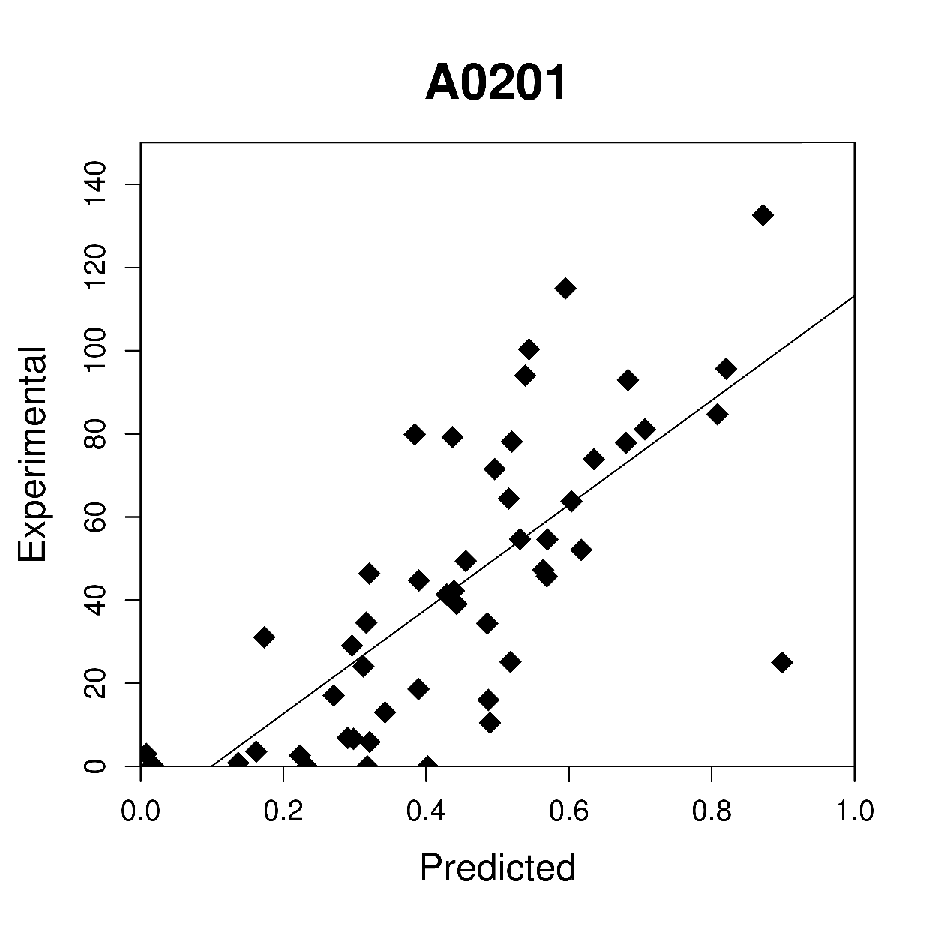
\includegraphics[width=7cm]{./Figures/chapter6/lower_res/exper_meta_1}%
\hspace{0cm}%
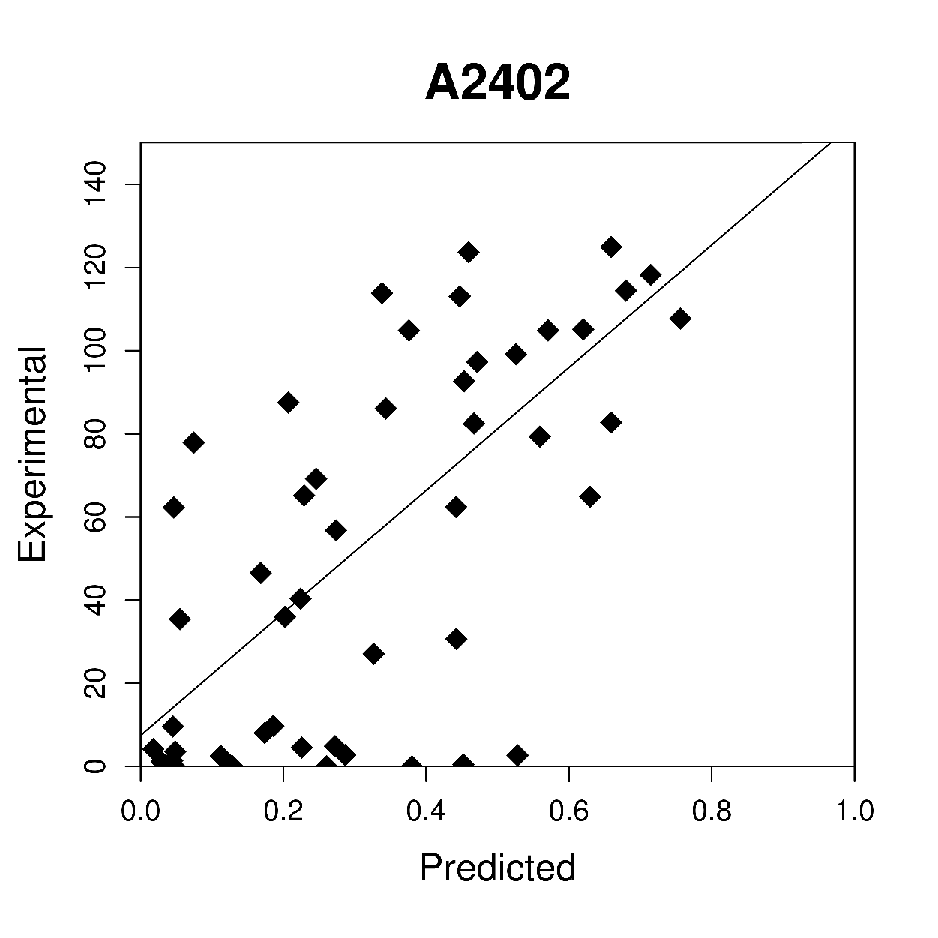
\includegraphics[width=7cm]{./Figures/chapter6/lower_res/exper_meta_2} \\
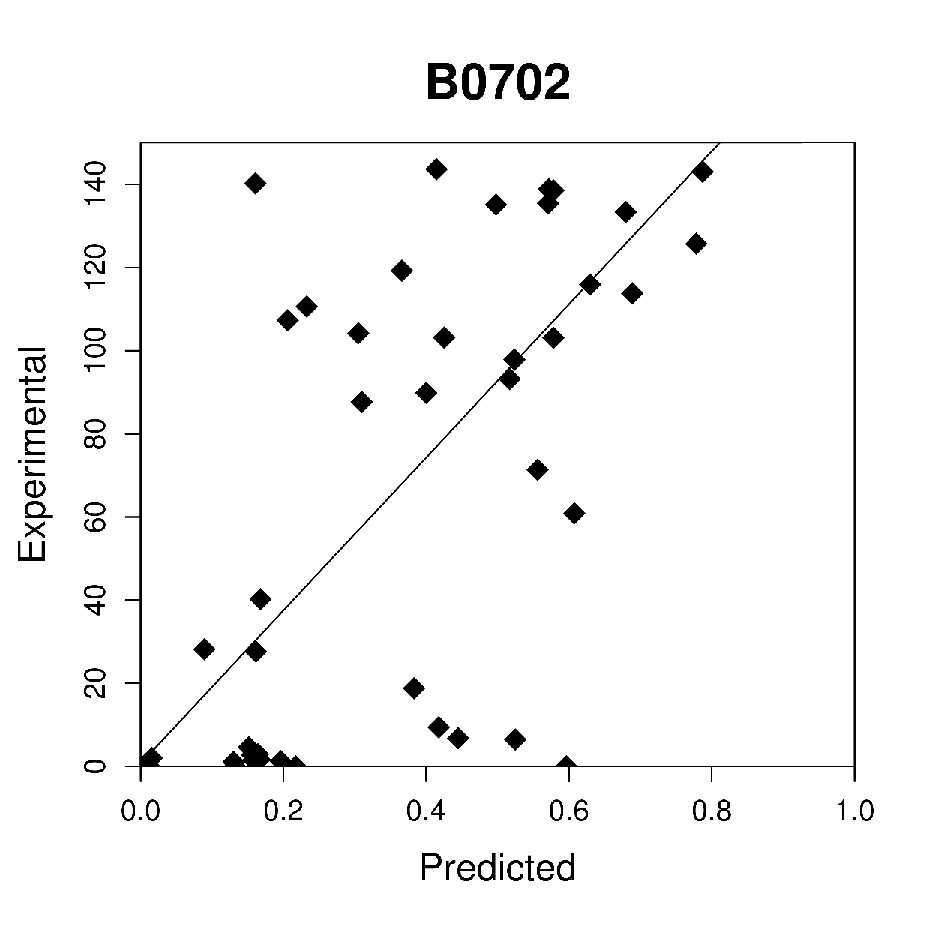
\includegraphics[width=7cm]{./Figures/chapter6/lower_res/exper_meta_3}%
\hspace{0cm}%
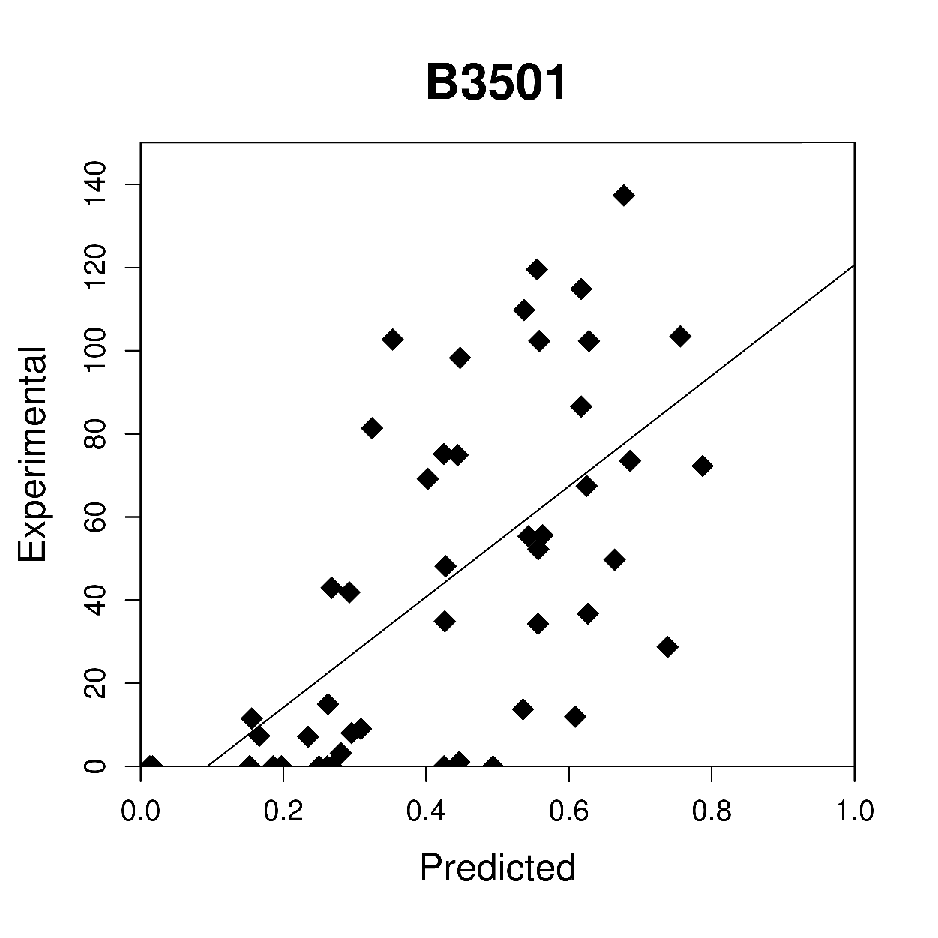
\includegraphics[width=7cm]{./Figures/chapter6/lower_res/exper_meta_4} \\
\caption[Experimental data for Metaserver]{The correlation between the experimentally measured binding affinities (\% binding compared to control peptide) and the predicted binding affinities ($1-\log _{50000} \left( \text{affinity} \right)$) of Metaserver for each of the 4 alleles analysed.}
\label{chapter6/figure1}
\end{figure}

\begin{figure}[htp]
\centering
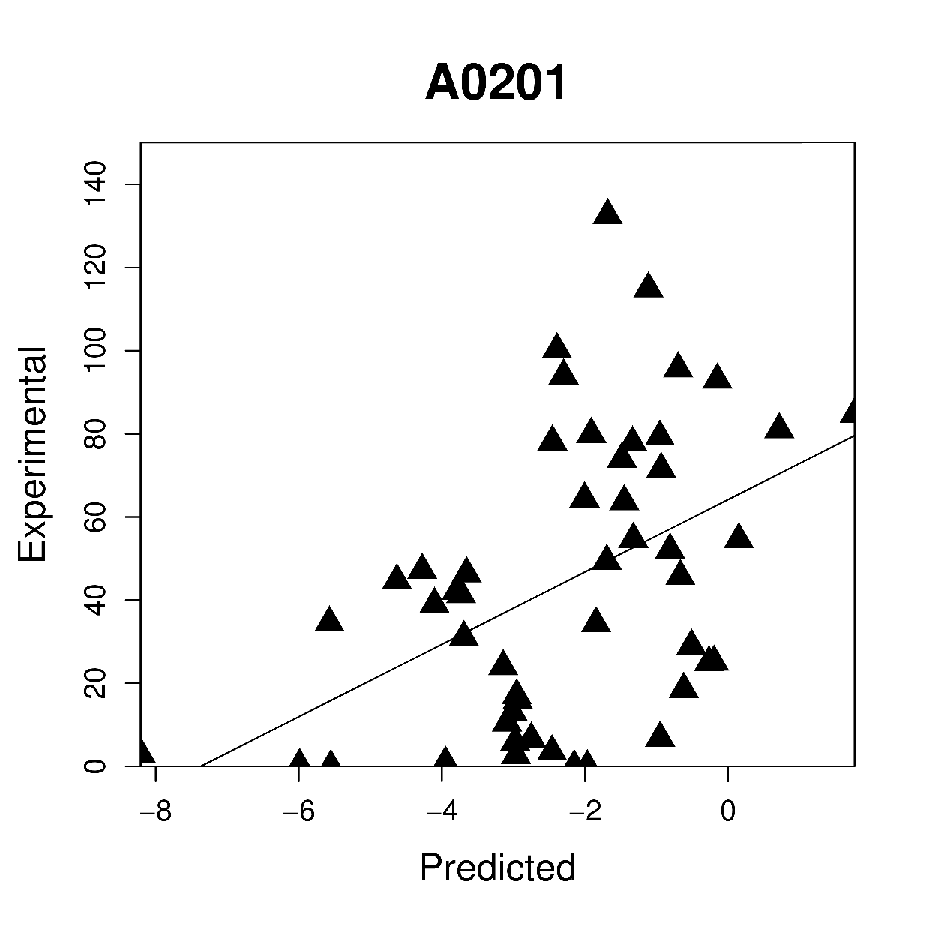
\includegraphics[width=7cm]{./Figures/chapter6/lower_res/exper_epi_1}%
\hspace{0cm}%
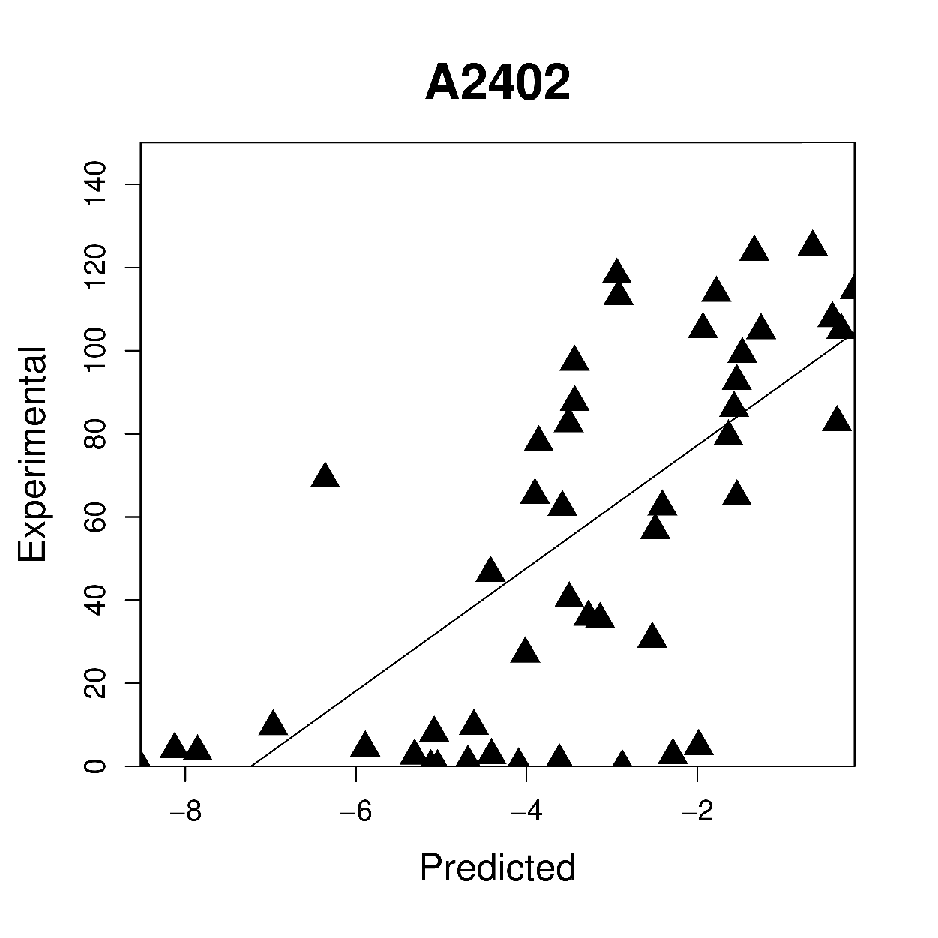
\includegraphics[width=7cm]{./Figures/chapter6/lower_res/exper_epi_2} \\
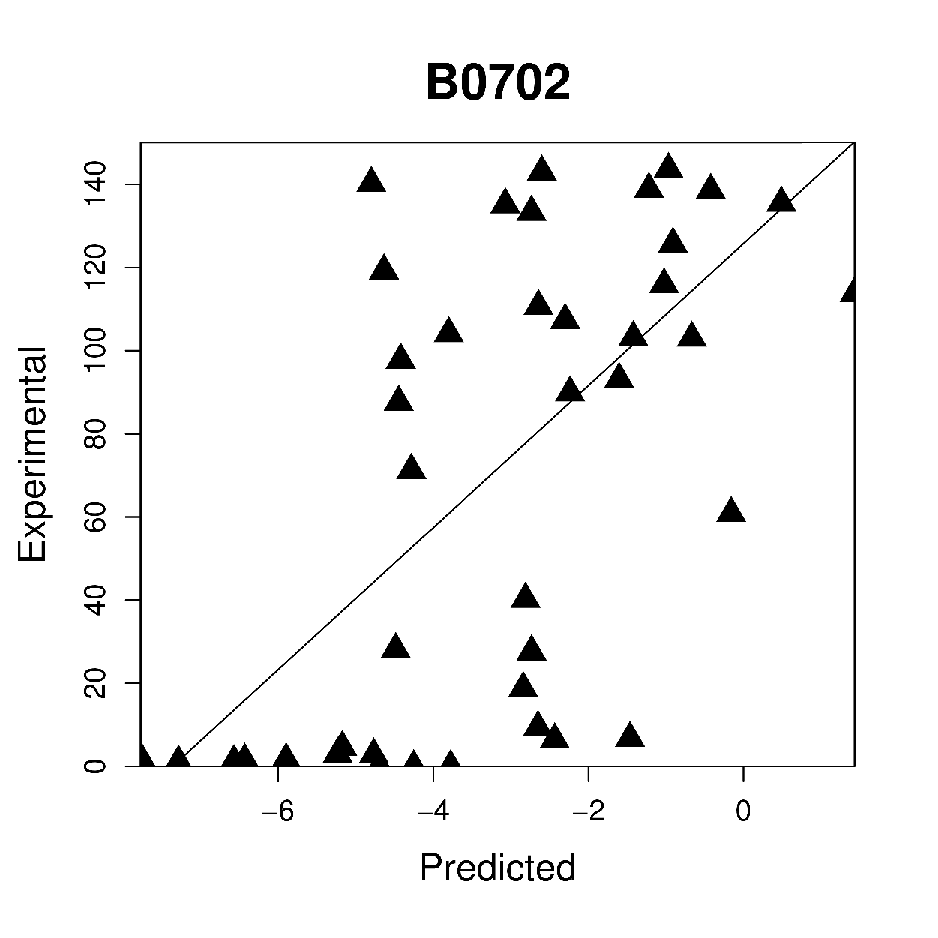
\includegraphics[width=7cm]{./Figures/chapter6/lower_res/exper_epi_3}%
\hspace{0cm}%
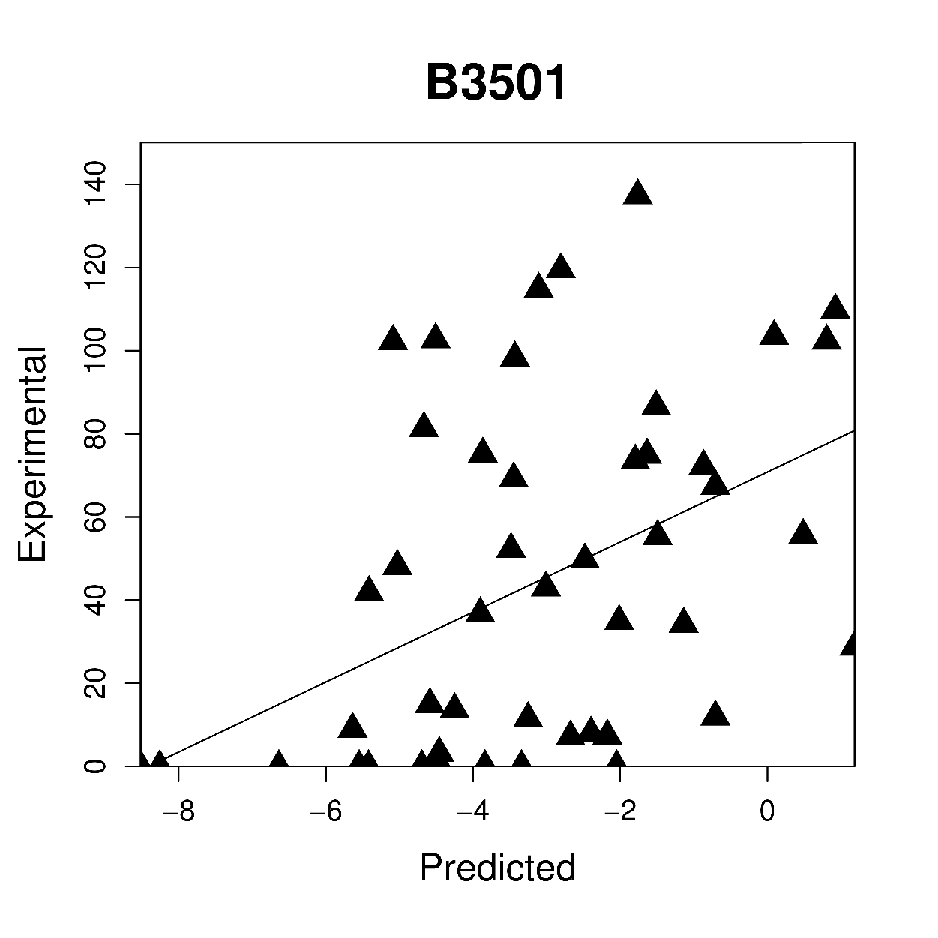
\includegraphics[width=7cm]{./Figures/chapter6/lower_res/exper_epi_4} \\
\caption[Experimental data for Epipred]{The correlation between the experimentally measured binding affinities (\% binding compared to control peptide) and the predicted binding affinities ($1-\log _{50000} \left( \text{affinity} \right)$) of Epipred for each of the 4 alleles analysed.}
\label{chapter6/figure2}
\end{figure}

\subsection{Protective class I alleles bind HBZ strongly}\label{Chapter6Result2}

A number of associations between HLA class I alleles and protection or disease risk in HTLV-I infection have been identified in a population in southern Japan \citep{Jeffery1999, Jeffery2000}. We performed a rigorous reanalysis of these associations for verification and refinement in \cref{Chapter3}. From this data, \gene{A*0201} and \gene{Cw*0801} were classed as protective alleles and \gene{B*5401} as a detrimental allele in the context of disease risk and proviral load. Hence, we started our analysis of HTLV-I epitopes with these alleles.

We compared the predicted HTLV-I peptide-binding affinities of \gene{A*0201} and \gene{Cw*0801}, with those of \gene{B*5401} (see Methods, \sref{MethodsChapter6Result2}). Peptides from the HTLV-I protein HBZ bound to HLA A*0201 and Cw*0801 significantly more strongly compared to B*5401 ($P = 0.0002$, Wilcoxon-Mann-Whitney; \fref{chapter6/figureExtra}, \tref{chapter6/tableExtra}). Repeating the analysis with another protective allele from the \gene{A*02} family, \gene{A*0206}, instead of \gene{A*0201} yielded identical conclusions ($P = 0.0007$, Wilcoxon-Mann-Whitney; data not shown). These $P$ values need to be treated with caution because the rank of the binding affinity of one HBZ peptide for A*0201 may not be independent of the rank of the binding affinity of a second peptide to A*0201 and similarly for Cw*0801 and B*5401. However, we also found that the difference in binding strength (i.e.~the rank of the top A*0201 binding peptide minus the rank of the top B*5401 binding peptide) was significantly greater for HBZ than for other HTLV-I proteins ($P < 0.001$, binomial test). This statistic is based only on the top binding peptide so it does not assume different peptides have independent binding affinity ranks. Henceforth, we only considered the top binding peptide to avoid the potential problem of dependence (see Methods, \sref{IndependenceRanks}).

\begin{figure}[htp]
\centering
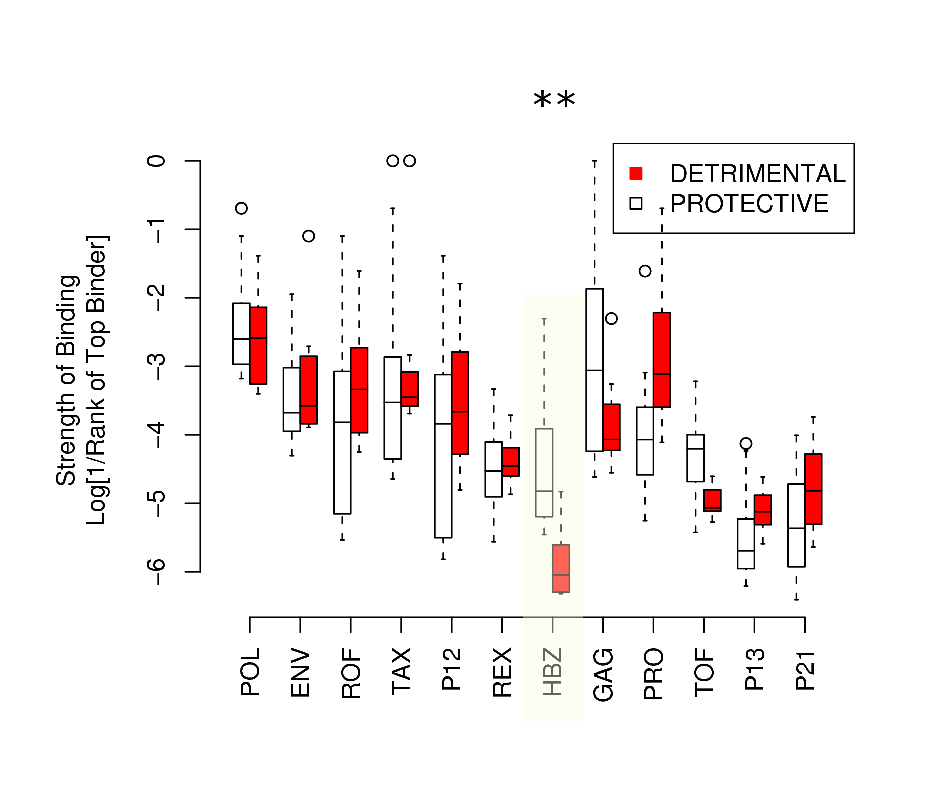
\includegraphics[width=14cm]{./Figures/chapter6/fig_2_edit}
\rule{35em}{0.5pt}
\caption[Protective class I alleles bind HBZ strongly]{The strength of binding of protective alleles (A*02/Cw*08) and detrimental alleles (B*54) across the 12 HTLV-I proteins. The y-axis gives strength of binding of the top 8 binding peptides from each protein. The level of significance indicated is corrected for multiple comparisons. All $P$ values are shown in \tref{chapter6/tableExtra}.}
\label{chapter6/figureExtra}
\end{figure}


\begin{table}[htp]
\begin{center}

\begin{tabular}{|c|c|}
\hline
Protein & Mann-Whitney 2-tailed $P$ value \bigstrut \\
\hline
Pol & 0.4999 \bigstrut[t] \\
Env & 0.5003 \\
Rof & 0.2091 \\
Tax & 0.4257 \\
P12 & 0.2978 \\
Rex & 0.5283 \\
HBZ & 0.0002 \\
Gag & 0.2572 \\
Pro & 0.0087 \\
Tof & 0.0131 \\
P13 & 0.0523 \\
P21 & 0.1200 \bigstrut[b] \\
\hline
\end{tabular}

\end{center}

\caption[Protective class I alleles bind HBZ strongly]{The $P$ values associated with \fref{chapter6/figureExtra}.}
\label{chapter6/tableExtra}
\end{table}

\subsection{Asymptomatic carriers bind HBZ more strongly than HAM/TSP patients}\label{Chapter6Result3}

Having established that the known protective HLA class I alleles bind to peptides from HBZ more strongly than the known detrimental allele, we examined peptide binding by all alleles in the Kagoshima cohort. We compared the predicted epitopes for asymptomatic carriers ($n = 202$) and HAM/TSP patients ($n = 230$) from the Kagoshima cohort. We predicted the HTLV-I peptides bound most strongly by each individual, given their HLA class I types and then tested for differences between the two subject groups (see Methods, \sref{MethodsChapter6Result3}). The results are illustrated in \fref{chapter6/figure3} and \tref{chapter6/table3}. One result remained highly statistically significant after correction for multiple comparisons and was consistent across both prediction methods: asymptomatic carriers have HLA class I alleles that bind more strongly to peptides from HBZ compared to HAM/TSP patients (Metaserver: $P = 0.0002$, Wilcoxon-Mann-Whitney. Epipred: $P < 0.0001$, Wilcoxon-Mann-Whitney; \fref{chapter6/figure3}). A bootstrap analysis was performed to confirm this result in both Metaserver and Epipred (\fref{chapter6/BootstrapMeta} and \fref{chapter6/BootstrapEpi}).

\begin{table}[htp]
\begin{center}

%\setlength{\extrarowheight}{1.5pt}
%\setlength{\tymin}{2cm}
%\tymax=\maxdimen
\begin{tabulary}{0.8\textwidth}{|l|p{1.5cm}|L|L|p{1.5cm}|L|L|}
\hline
& \multicolumn{3}{c|}{Metaserver} & \multicolumn{3}{c|}{Epipred} \\
\hline
Protein & $P$ value (2 tailed) & Group with strongest binding & Significance after correction & $P$ value (2 tailed) & Group with strongest binding	& Significance after correction \\
\hline
pol & 0.0005 & AC & ** & 0.0744 & AC & - \\
env & 0.0019 & HAM & * & 0.7203 & HAM & - \\
rof & 0.0023 & HAM & * & 0.0127 & HAM & - \\
tax & 0.3320 & AC & - & 0.8320 & HAM & - \\
p12 & 0.0168 & HAM & - & 0.0940 & HAM & - \\
rex & 0.4706 & AC & - & 0.7639 & AC & - \\
HBZ & 0.0002 & AC & ** & 0.000002 & AC & *** \\
gag & 0.0011 & AC & * & 0.1265 & HAM & - \\
pro & 0.0970 & HAM & - & 0.0143 & HAM & - \\
tof & 0.4111 & HAM & - & 0.0256 & HAM & - \\
p13 & 0.8524 & AC & - & 0.7308 & AC & - \\
p21 & 0.0341 & AC & - & 0.0018 & HAM & * \\
\hline
\end{tabulary}
\end{center}

\caption[The binding strength to all HTLV-I proteins of HAM/TSP and AC alleles]{The differences in the strength of binding of the alleles between AC and HAM/TSP patients to each of the 12 HTLV-I proteins.}
\label{chapter6/table3}
\end{table}

\begin{figure}[htp]
\centering
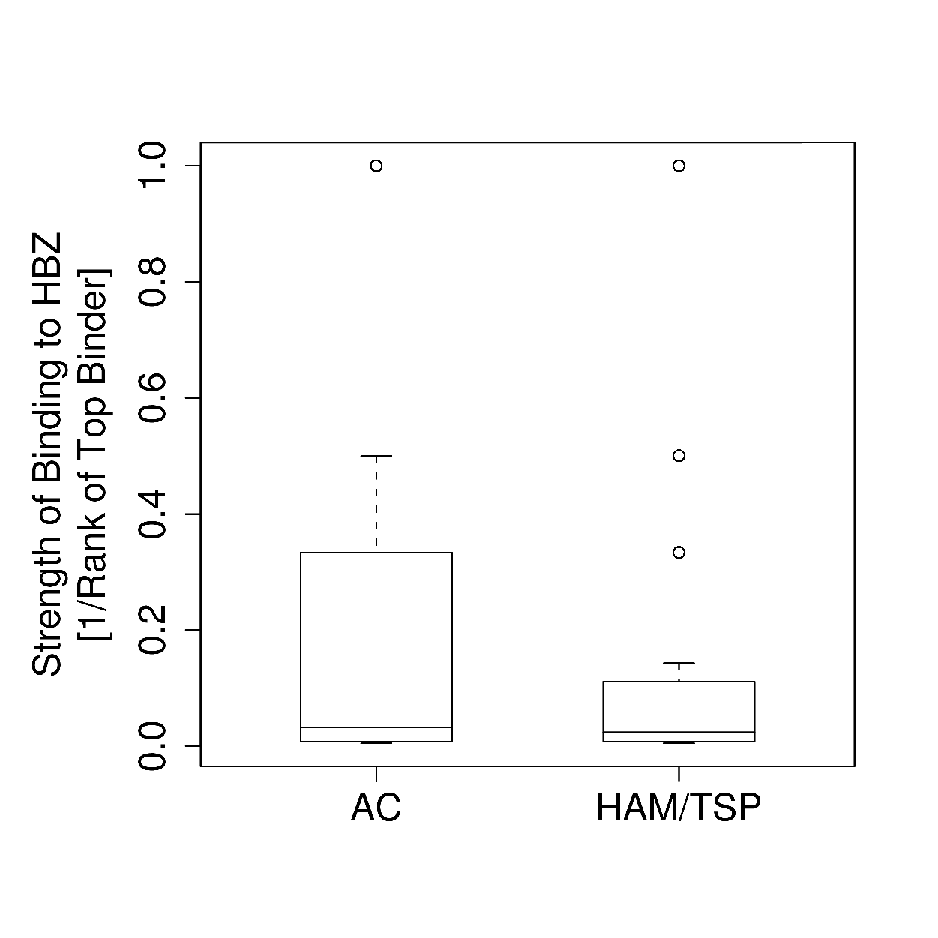
\includegraphics[width=7cm]{./Figures/chapter6/lower_res/fig_3_meta}%
\hspace{0cm}%
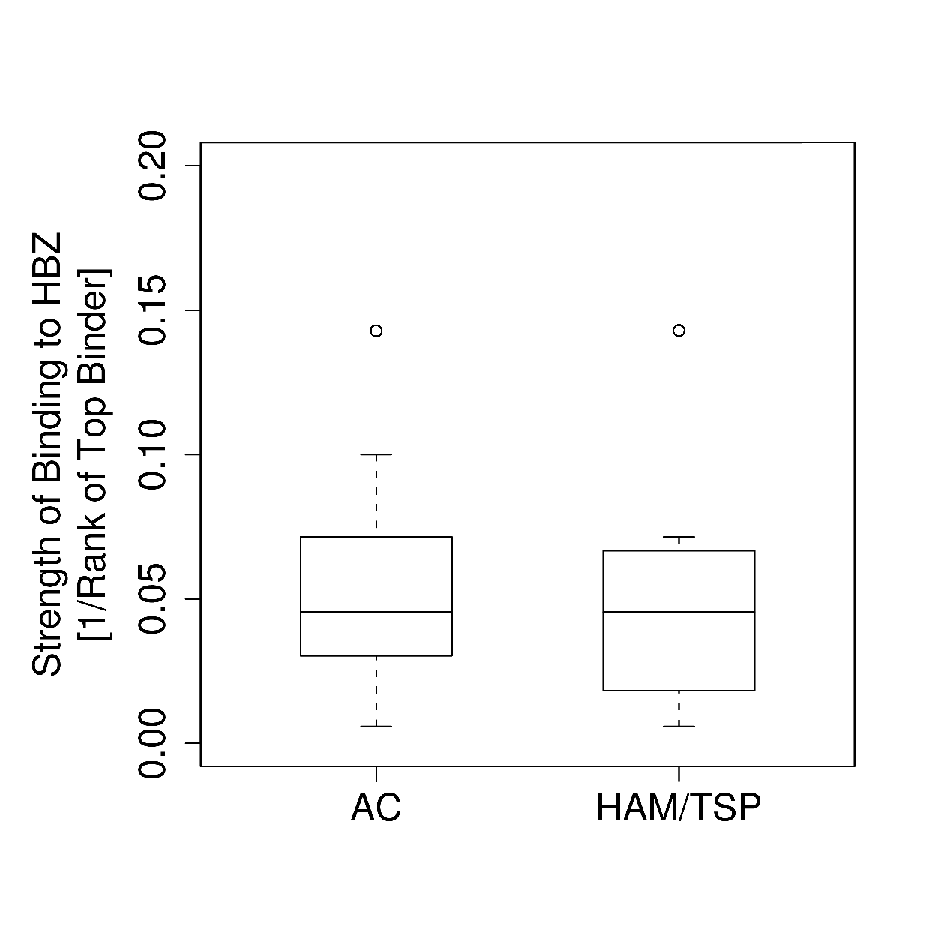
\includegraphics[width=7cm]{./Figures/chapter6/lower_res/fig_3_epi} \\
\caption[The strength of binding to HBZ]{The strength of binding of the HLA class I alleles of asymptomatic carriers and HAM/TSP patients to HBZ. Asymptomatic carriers have HLA class I alleles that bind HBZ significantly more strongly than HAM/TSP patients (Metaserver, left panel: $P = 0.0002$. Epipred, right panel: $P = 2 \times 10^{-6}$).}
\label{chapter6/figure3}
\end{figure}

To test whether this association was caused solely by the known protective and detrimental HLA alleles, the analysis for HBZ was repeated excluding A*02 and B*54. The results showed that, amongst the HLA-A alleles, A*02 was responsible for the protective effect, whereas in HLA-B more than one allele contributed significant effects. Overall, strong binding of HBZ peptides was associated with asymptomatic status, even when A*02, B*54 and Cw*08 were excluded from the analysis (Metaserver: $P = 0.04$, Wilcoxon-Mann-Whitney. Epipred: $P = 0.006$, Wilcoxon-Mann-Whitney; \tref{chapter6/table2}).

\begin{table}[htp]
\begin{center}

\newcommand{\rr}{\raggedright}
\newcommand{\tn}{\tabularnewline}

{
	\renewcommand{\arraystretch}{1.2}
	\begin{tabular}{|l|l|p{2.5cm}|p{4cm}|}
	\hline
	\multicolumn{2}{|c|}{} & \rr Whole cohort ($N=202, 230$) & \rr Excluding A*02 \& B*54 ($N=84,116$) \tn
	\hline
	\multirow{3}{*}{Metaserver} & A alleles & 0.006 & 0.81 \tn
	& B alleles & 0.001 & 0.01 \tn
	& Combined & 0.0005 & 0.04 \tn
	\hline
	\multirow{3}{*}{Epipred} & A alleles & 0.0009 & 0.72 \tn
	& B alleles & 0.0002 & 0.001 \tn
	& Combined & 0.000001 & 0.006 \tn
	\hline
	\end{tabular}
}	
	
\end{center}

\caption[The binding strength to HBZ for HAM/TSP and AC individuals]{The difference in binding strength to HBZ between HAM/TSP patients and asymptomatic carriers. The first column gives the $P$ values of the Wilcoxon-Mann-Whitney tests for the A and B loci. The second column repeats this analysis excluding individuals with either the A*02 or B*54 alleles.}
\label{chapter6/table2}
\end{table}

\begin{figure}[p]
\centering
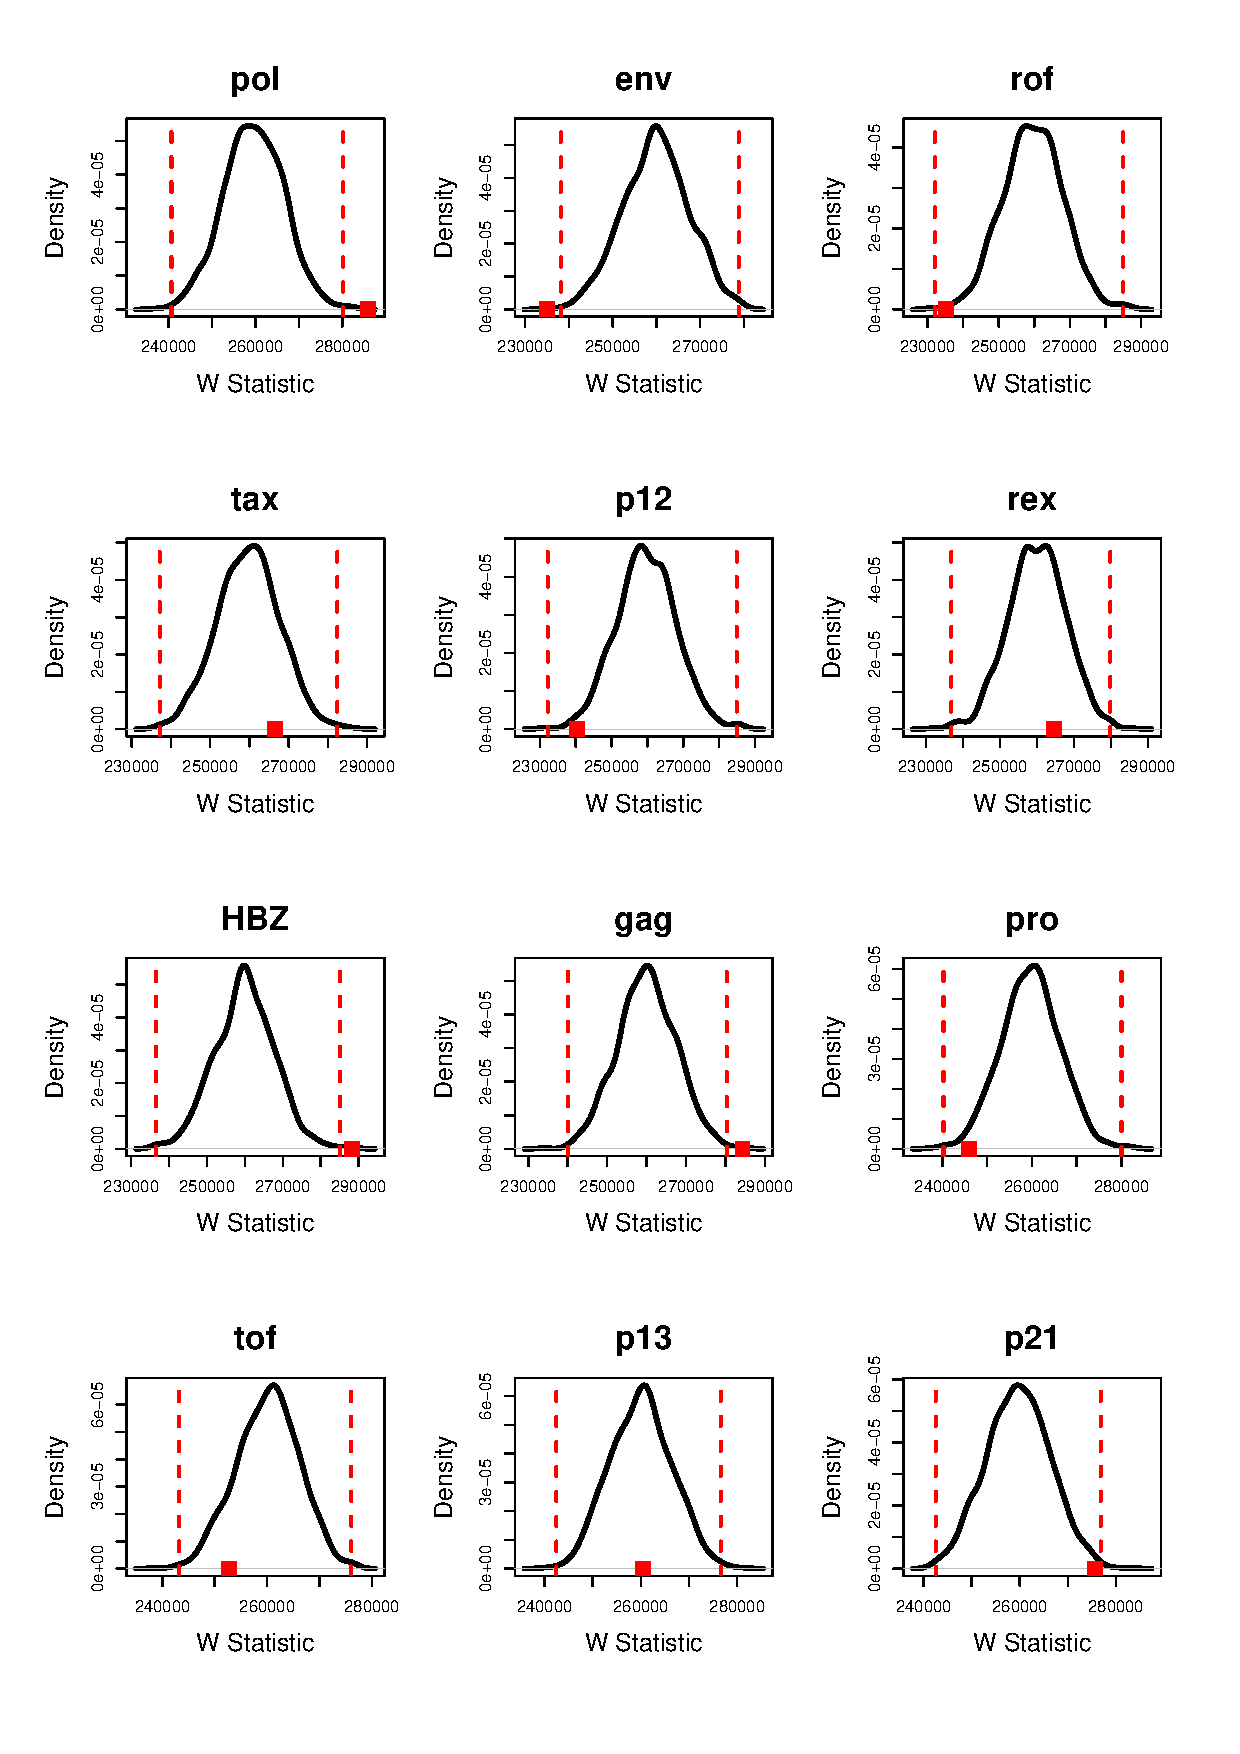
\includegraphics[width=14cm]{./Figures/chapter6/test/bootstrap_meta} \\
\caption[The bootstrap analysis for Metaserver]{A bootstrapping method to validate the conclusion of \sref{Chapter6Result3} (ACs bind HBZ more strongly than HAM/TSP patients). The 432 individuals of the Kagoshima cohort were randomly assigned to an `AC' and `HAM/TSP' group. The Mann-Whitney test was then performed on these groups. This was repeated 1,000 times and the density plot of the resultant W statistics of each test was plotted, together with the W statistic from the `true' test (red dot). The dotted lines represent the 2-tailed levels of significance after the Bonferroni adjustment for multiple comparisons. As can be seen from the HBZ graph, the W statistic value is still significantly different from the null distribution of bootstrapped W statistic values. This analysis for Metaserver was repeated for Epipred in \fref{chapter6/BootstrapEpi}.}
\label{chapter6/BootstrapMeta}
\end{figure}

\begin{figure}[p]
\centering
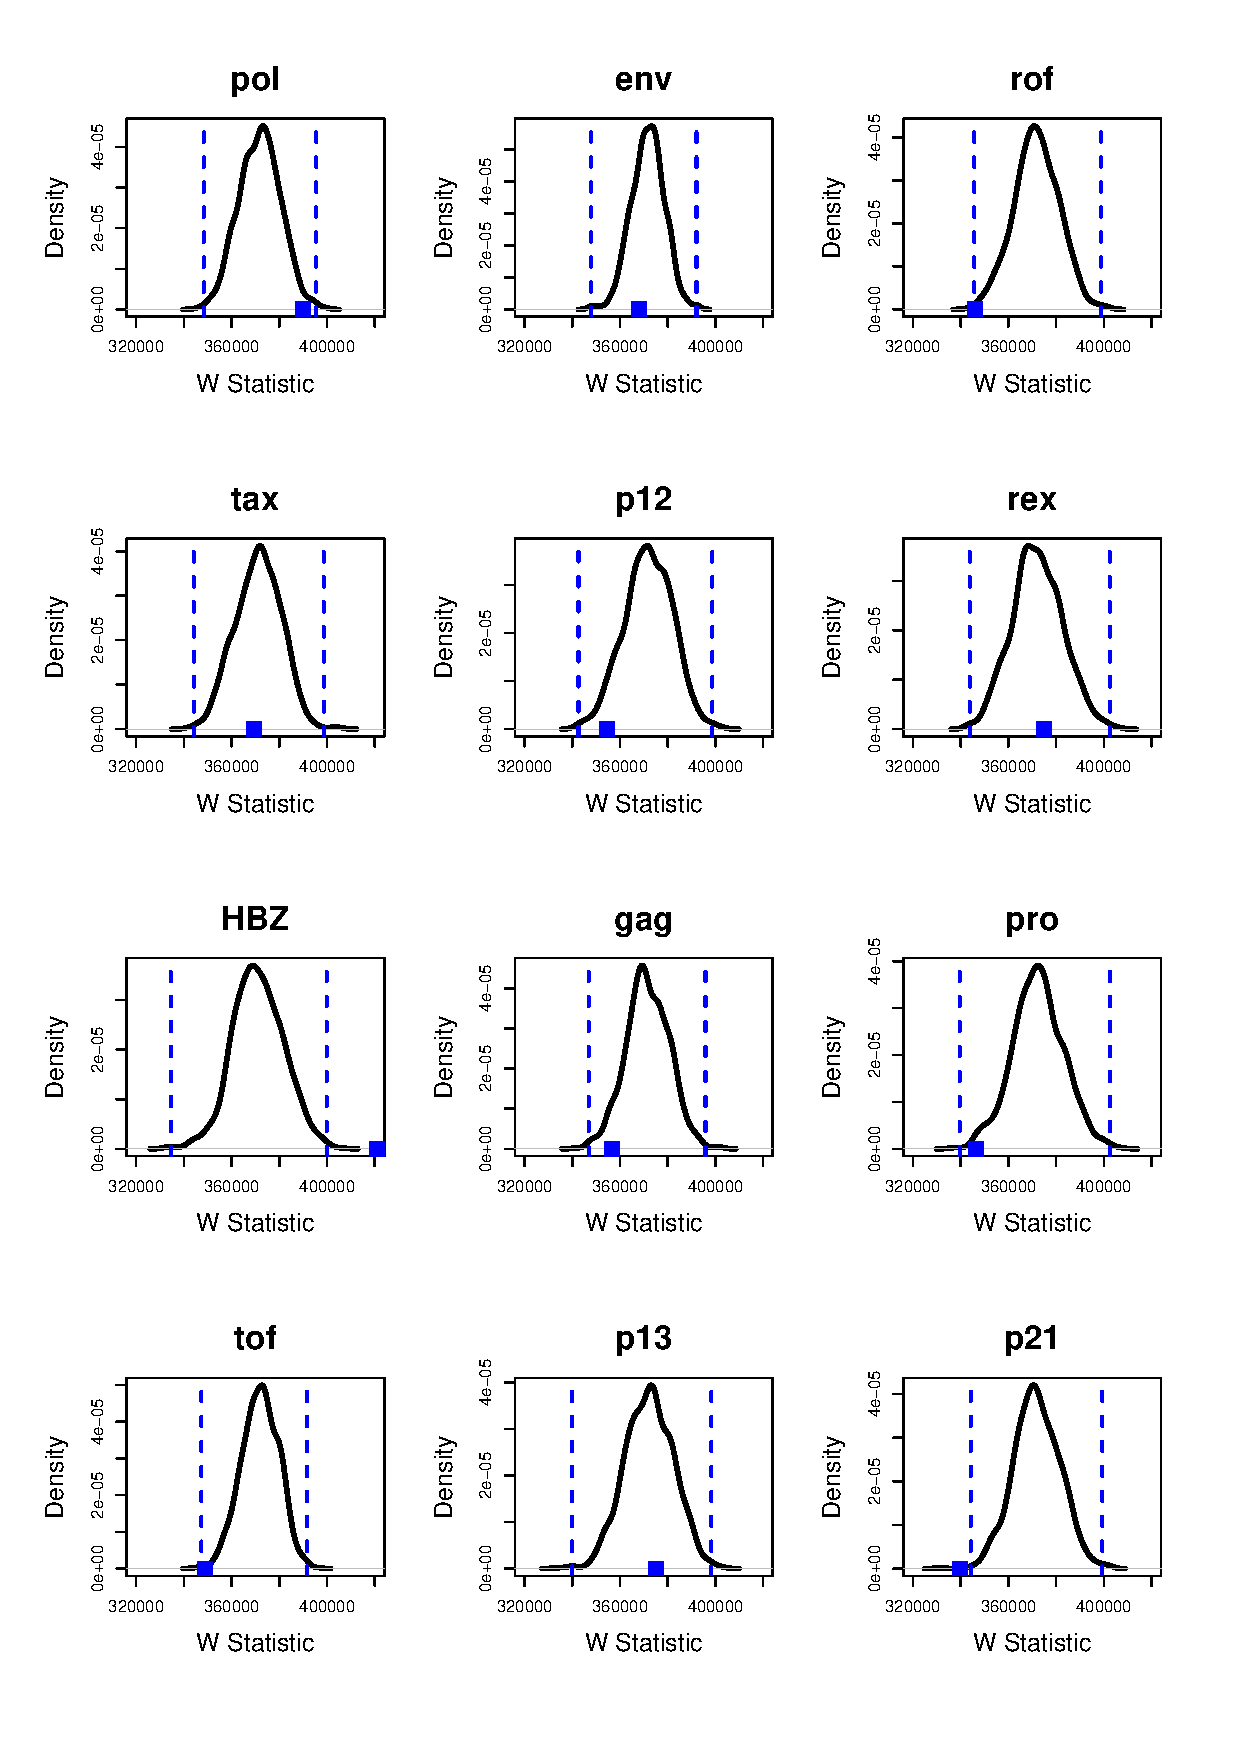
\includegraphics[width=14cm]{./Figures/chapter6/test/bootstrap_epi} \\
\caption[The bootstrap analysis for Epipred]{The bootstrap analysis for Epipred, described in \fref{chapter6/BootstrapMeta}. The W statistic value for HBZ is significantly different from the null distribution of bootstrapped W statistic values.}
\label{chapter6/BootstrapEpi}
\end{figure}

\subsection{Individuals whose HLA class I genotype predisposed them to bind HBZ peptides strongly had a significantly lower proviral load}\label{Chapter6Result4}

Next we investigated why strong binding of HBZ peptides was associated with remaining asymptomatic. One of the best predictors of HAM/TSP is a high proviral load of HTLV-I \citep{Nagai1998}. We therefore tested the hypothesis that strong predicted binding of HBZ peptides was associated with a lower proviral load. The number of alleles that each individual possessed that strongly bound peptides from HBZ was plotted against their proviral load (see Methods, \sref{MethodsChapter6Result4}). We found that the number of HLA Class I alleles that an individual had that strongly bound HBZ peptides was significantly negatively correlated with their proviral load (Metaserver: $P = 0.016$, Spearman�s rank correlation. Epipred: $P = 0.1$, Spearman�s rank correlation; \fref{chapter6/figure4}). We tested this correlation independently in HAM/TSP patients and asymptomatic carriers and then combined the $P$ values (rather than simply testing the whole cohort), so this result does not follow trivially from our previous observation than asymptomatic carriers bind HBZ significantly more strongly than HAM/TSP patients. An alternative metric, the binding strength of the top HBZ-binding peptide to each allele instead of the number of strongly binding alleles, yielded an identical conclusion i.e.~there was a significant negative correlation between the proviral load and the strength of binding to HBZ peptides (Metaserver: $P = 0.008$, Spearman�s rank correlation. Epipred: $P = 0.003$, Spearman�s rank correlation).

\begin{figure}[htp]
\centering
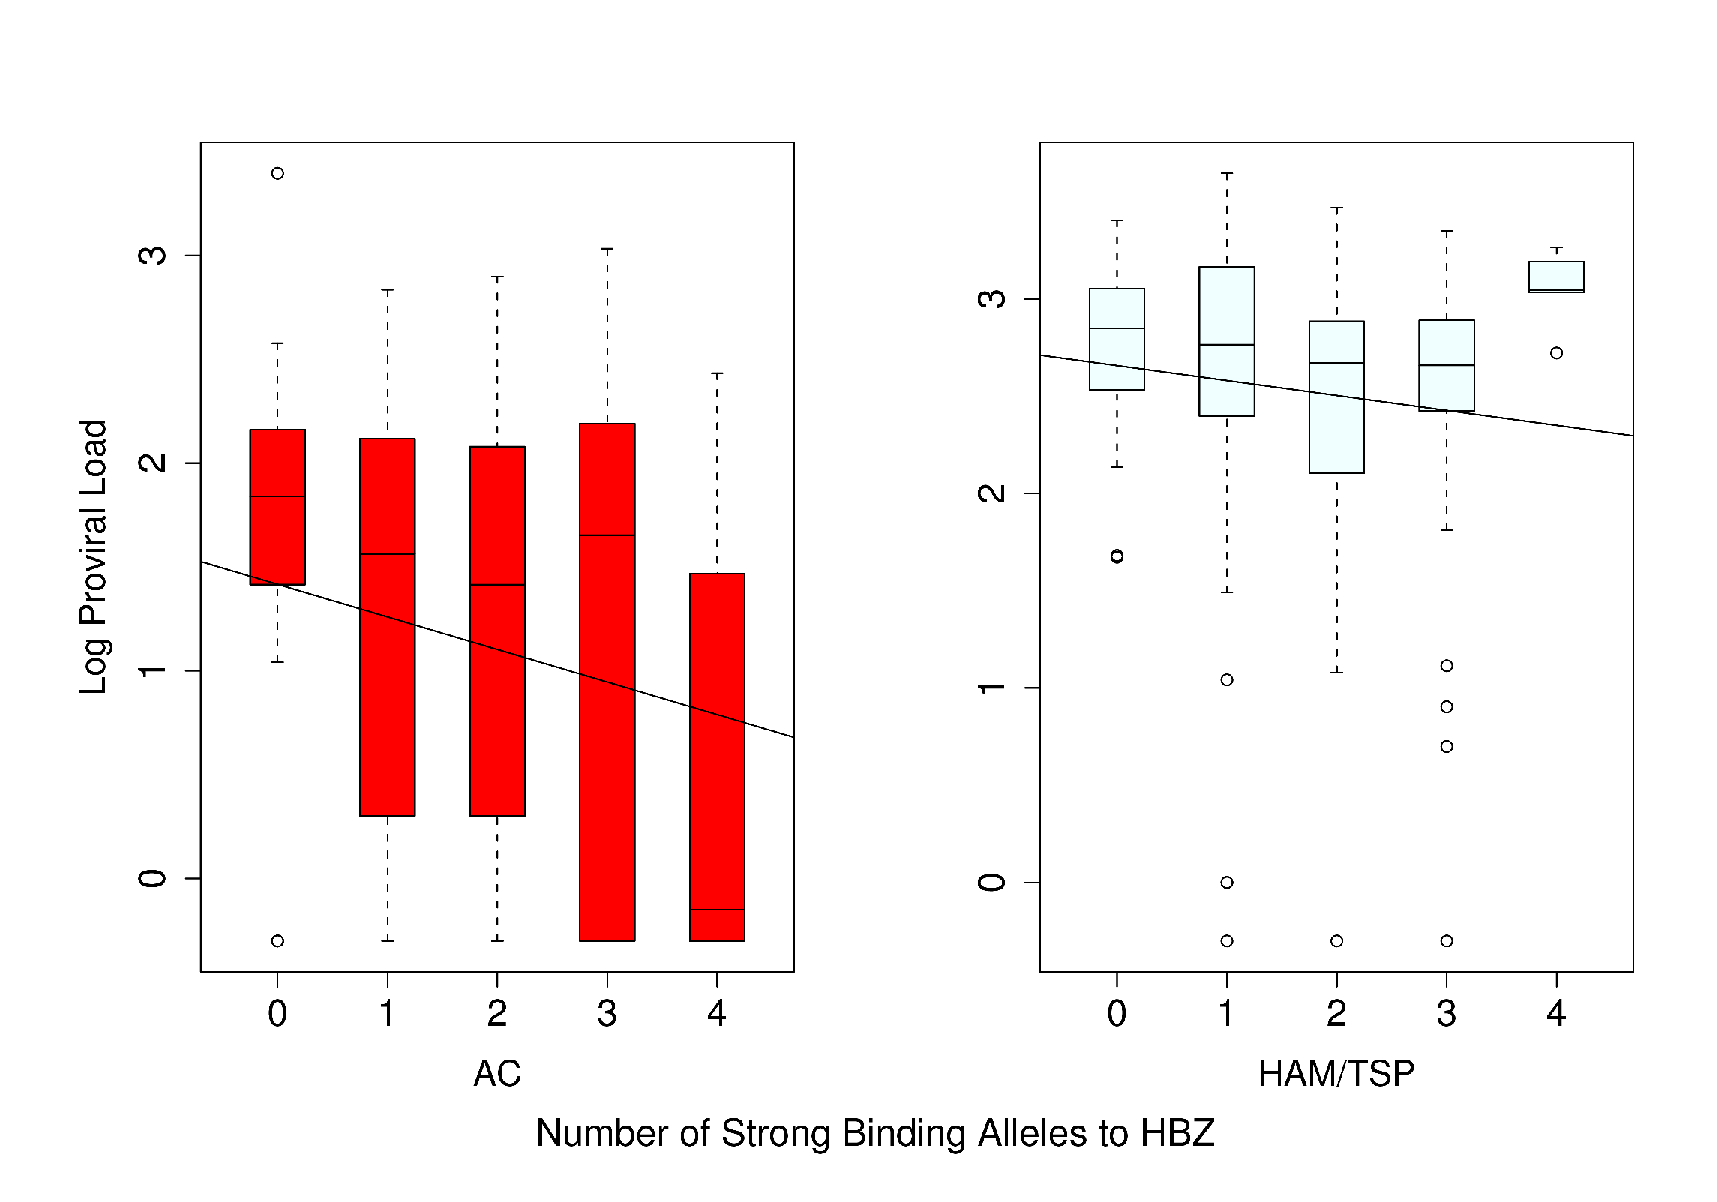
\includegraphics[width=14cm]{./Figures/chapter6/lower_res/fig_4_meta} \\
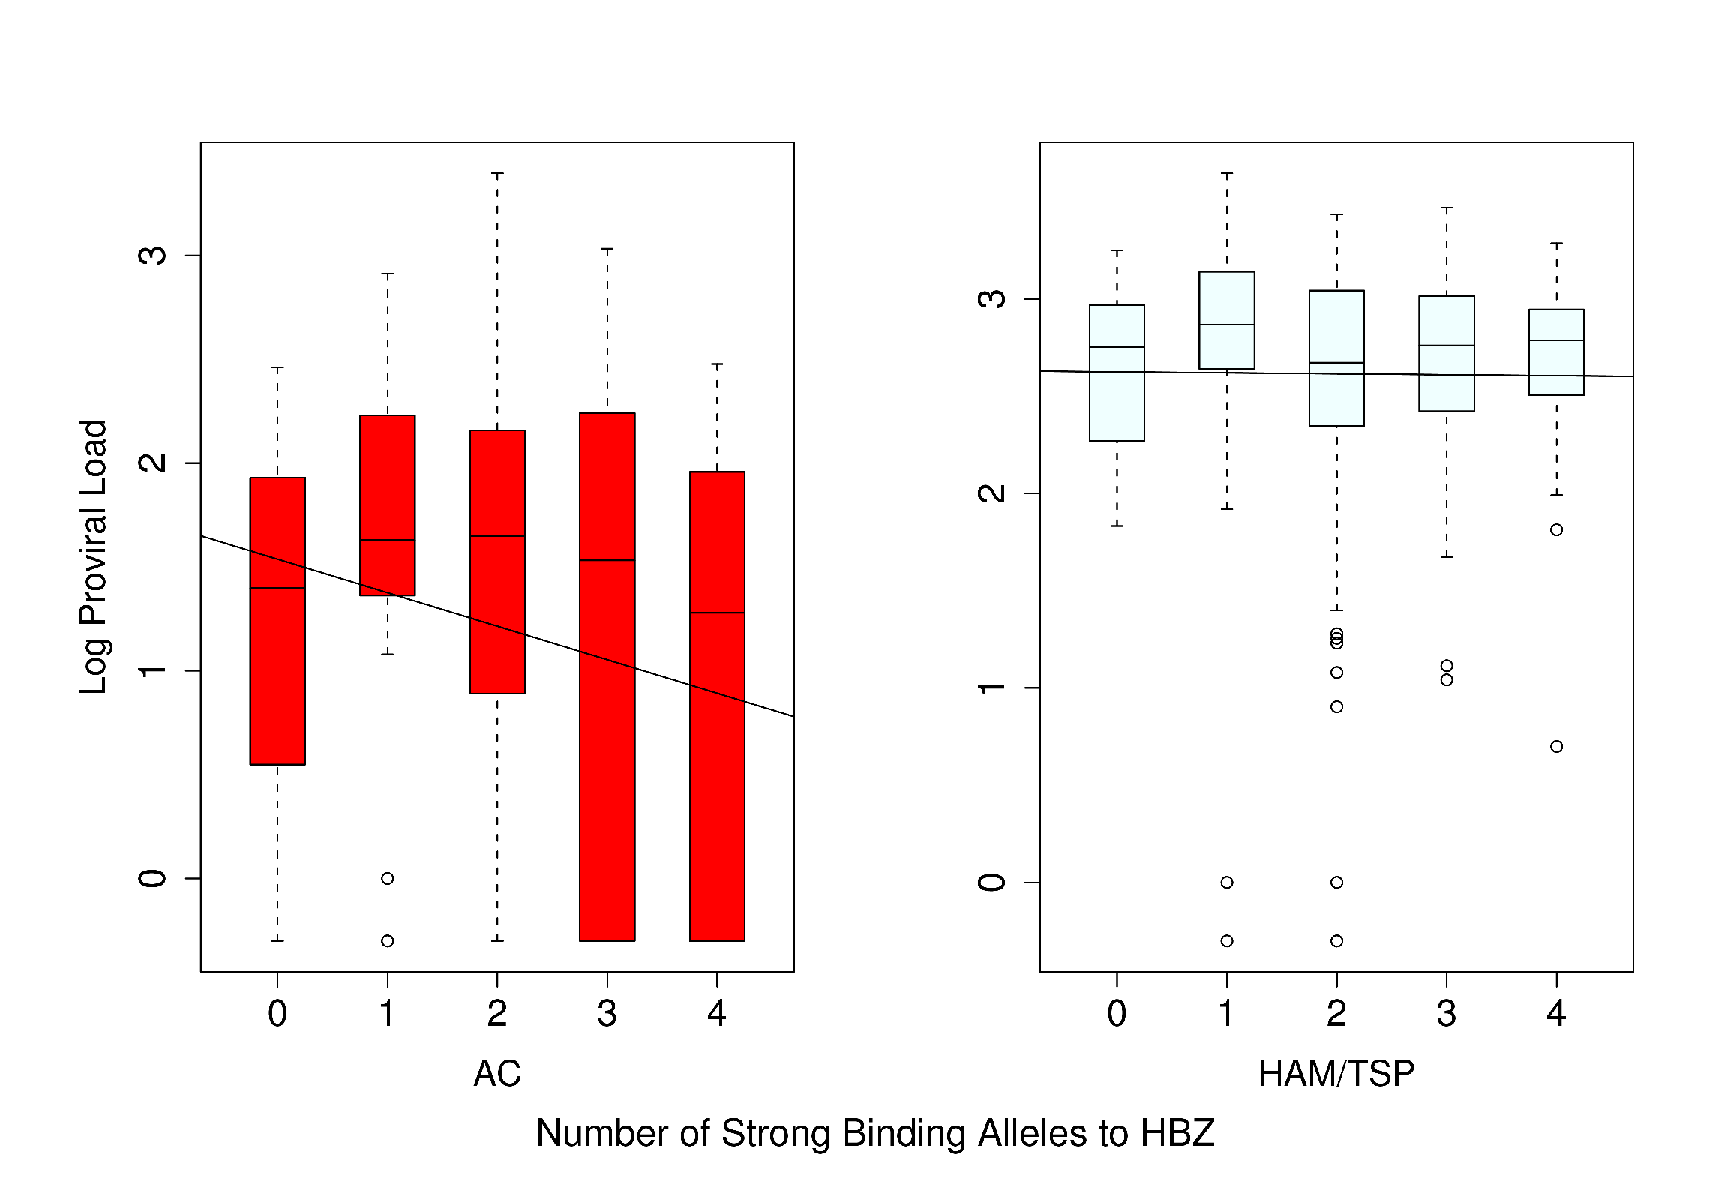
\includegraphics[width=14cm]{./Figures/chapter6/lower_res/fig_4_epi} \\
\caption[The strength of binding to HBZ and proviral load]{The count of strong binding alleles to HBZ per individual against their proviral load in AC and HAM/TSP groups. The number of strong binders to HBZ is significantly negatively correlated with proviral load (Metaserver, top panel: $P = 0.016$. Epipred, bottom panel: $0.1$).}
\label{chapter6/figure4}
\end{figure}

\subsection{HBZ Peptide Binding is a Consistent Predictor of Proviral Load}\label{chapter6/results/pred}

Next we compared our peptide-binding analysis of HLA class I genotype with a traditional frequency-based ``presence or absence of an allele'' analysis. Previously a ``traditional'' analysis yielded inconsistent results \citep{Jeffery1999, Jeffery2000, Vine2002}. For example, A*02 was a significant predictor of load in ACs but not in patients with HAM/TSP. We therefore directly compared the ability of the two methods to predict proviral load in ACs and HAM/TSP patients (\tref{chapter6/table4}). This analysis showed that whilst binding HBZ was a significant predictor of proviral load in both ACs and HAM/TSP patients ($P = 0.001$, $P = 0.017$), HLA-A*02 (presence/absence) was a significant predictor in ACs only ($P = 0.01$) and HLA-B*54 for HAM/TSP patients only ($P = 0.019$). The proportion of variance in proviral load explained was marginally higher for the peptide binding analysis. The observation that HBZ binding strength correlated with proviral load in both ACs and HAM/TSP patients suggests that peptide binding is the more fundamental predictor than HLA genotype. Further details of the predictive strength of peptide binding for proviral load and disease risk is described in \aref{AppendixC}, \sref{appendixc/log}.  

\begin{table}[htp]
\begin{center}

\begin{tabular}{|l|l|l|l|l|l|l|}
\hline
& \multicolumn{3}{c|}{Binding (A and B only)} & \multicolumn{3}{c|}{Genotype (A and B only)} \bigstrut \\
\hline
\multirow{3}{*}{AC Proviral Load} & HBZ & 0.001 & *** & \multirow{2}{*}{A*02} & \multirow{2}{*}{0.01} & \multirow{2}{*}{**} \bigstrut[t] \\
& Pro & 0.013 & * & & & \bigstrut[b] \\
\cline{2-7}
& \multicolumn{3}{c|}{$R^2 = 0.054$} & \multicolumn{3}{c|}{$R^2 = 0.034$} \bigstrut \\
\hline
\multirow{2}{*}{HAM/TSP Proviral Load} & HBZ & 0.017 & * & B*54 & 0.019 & * \bigstrut \\
\cline{2-7}
& \multicolumn{3}{c|}{$R^2 = 0.026$} & \multicolumn{3}{c|}{$R^2 = 0.025$} \bigstrut \\
\hline
\end{tabular}
\end{center}

\caption[Multiple regression models predicting proviral load]{The significant predictors and their associated P values for each of the multiple regression models of proviral load.}
\label{chapter6/table4}
\end{table}

\subsection{Proteins whose peptides are bound strongly by asymptomatic carriers are those associated with a lower proviral load}\label{chapter6/resultsProt}

In the work above we established that the HTLV-I protein that is associated with the most significant reduction in HAM/TSP risk when bound by HLA class I molecules (i.e.~HBZ, \tref{chapter6/table3}) is also, independently, associated with a significant reduction in proviral load when bound (\fref{chapter6/figure4}). We wished to investigate whether this relationship held across all proteins. We ranked each HTLV-I protein by the following criteria: 

\begin{enumerate}
\item Is strong binding of peptides from this protein associated with a lower HAM/TSP prevalence? 
\item Is strong binding of peptides from this protein associated with a lower proviral load (tested independently in AC and HAM/TSP groups and then recombined, to avoid trivial associations)?
\end{enumerate}

\tref{chapter6/table2HypothRank} illustrates this concept. The first column ranks the HTLV-I proteins according to whether they were bound more strongly by asymptomatic carriers or HAM/TSP patients (\fref{chapter6/figure5Meta} x-axis; at the extremes ACs were significantly more likely to bind peptides from HBZ, HAM/TSP patients were significantly more likely to bind peptides from Env). This list could be viewed as the ``rank order of targets for a vaccine designed to reduce HAM/TSP risk''. The second column ranks the proteins according to whether binding their peptides was associated with a lower proviral load (\fref{chapter6/figure5Meta}, y-axis; at the extremes binding of HBZ was associated with a significantly lower proviral load, binding of Env was associated with a significantly higher proviral load). This list could be viewed as the ``rank order of targets for a vaccine designed to reduce proviral load''.  

We then compared these two sets of ranks and found them to be strongly positively correlated (Metaserver: $R_S = 0.86$, $P = 0.0005$, Spearman�s rank correlation; \fref{chapter6/figure5Meta}. Epipred: $R_S = 0.66$, $P = 0.02$, Spearman�s rank correlation; \fref{chapter6/figure5Epi}). That is, proteins whose peptides are bound strongly by asymptomatic carriers are, independently, those associated with a lower load when bound. This observation has two important implications. Firstly, HLA class I binding of peptides from different proteins has a differential impact on both proviral load and HAM/TSP risk. Secondly, the fact that across all alleles and across all proteins, peptide binding associated with immune control (reduced proviral load) is strongly correlated with prevention of HAM/TSP is the strongest evidence yet that the CD8$^+$ T cell response can have a beneficial role in HTLV-I infection.

\begin{table}[htp]
\centering
\begin{tabular}{|c|c|c|}
\hline
& \multicolumn{2}{c|}{Targeting this protein is associated with:} \bigstrut \\
\hline
& Reduced HAM/TSP Frequency & Reduced Proviral Load \bigstrut \\
\hline
\multirow{3}{*}{\begin{sideways}Best\end{sideways}} & HBZ & Gag \bigstrut[t] \\
& Pol & HBZ \\
& Gag & Pol \\
\multirow{6}{*}{$\downarrow$} & P21 & Rex \\
& Tax & Tof \\
& Rex & P21 \\
& P13 & Pro \\
& Tof & Tax \\
& Pro & P13 \\
\multirow{3}{*}{\begin{sideways}Worst\end{sideways}} & P12 & P12 \\
& Rof & Rof \\
& Env & Env \bigstrut[b]\\
\hline
\end{tabular}
\caption[The rank order of HTLV-I protein targets]{The rank order of targeting HTLV-I proteins according to their potential to reduce the risk of HAM/TSP (first column) and reduce proviral load (second column).}
\label{chapter6/table2HypothRank}
\end{table}

\begin{figure}[htp]
\centering
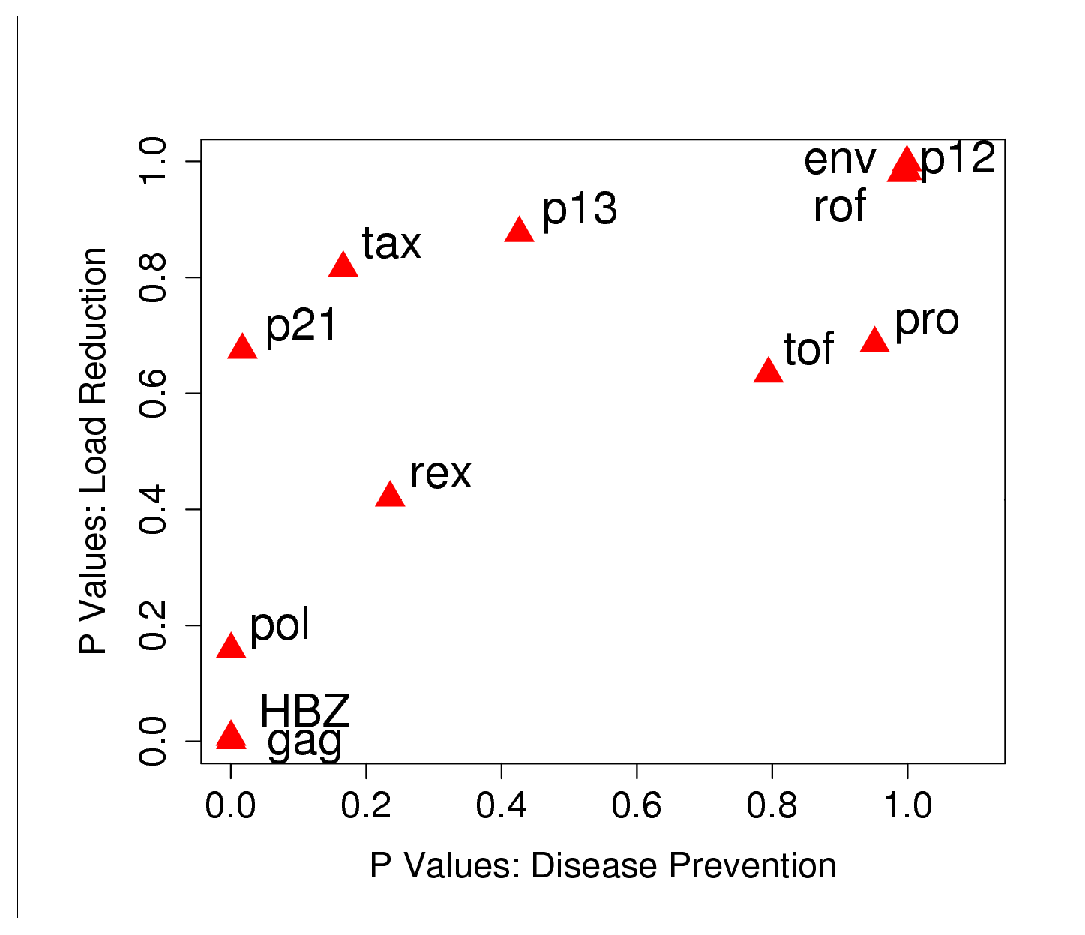
\includegraphics[width=14cm]{./Figures/chapter6/lower_res/fig_5_meta}
\rule{35em}{0.5pt}
\caption[The correlation of hypotheses for Metaserver]{The correlation between the $P$ values of the 1-tailed hypotheses: targeting this protein is associated with a lower proviral load and targeting this protein is associated with a lower HAM/TSP prevalence ($R_S=0.86$, $P = 0.0005$). In addition to HBZ, Gag also produced significant results in this analysis (it was significantly associated with a lower HAM/TSP prevalence ($P = 0.0005$) and a lower proviral load ($P = 0.002$)). However, we did not focus on this result as it was not repeated independently with Epipred.}
\label{chapter6/figure5Meta}
\end{figure}

\begin{figure}[htp]
\centering
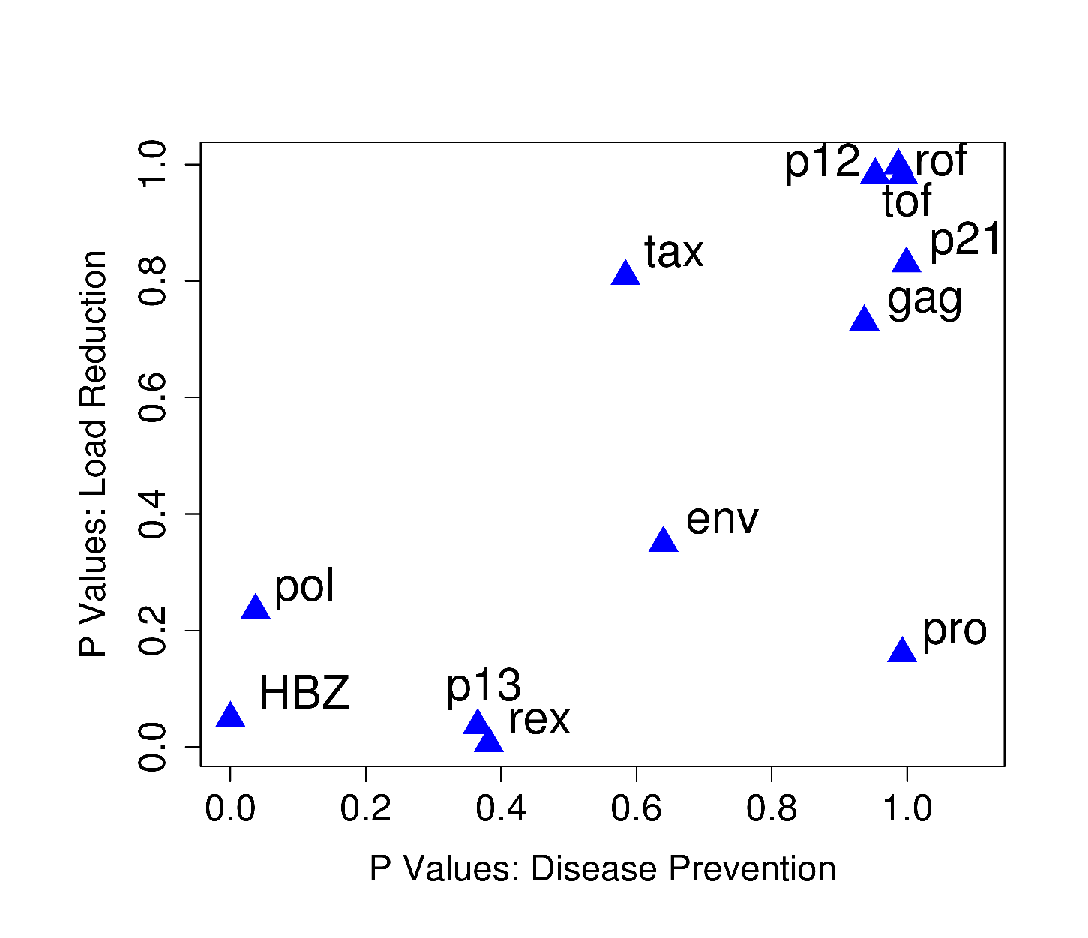
\includegraphics[width=14cm]{./Figures/chapter6/lower_res/fig_5_epi}
\rule{35em}{0.5pt}
\caption[The correlation of hypotheses for Epipred]{The correlation between the $P$ values of the 2 hypotheses: targeting this protein is associated with a reduction in HAM/TSP prevalence and targeting this protein is associated with a reduction in proviral load ($R_S=0.66$, $P = 0.02$). Epitope binding predictions made using Epipred.}
\label{chapter6/figure5Epi}
\end{figure}

\subsection{The Prevented Fraction of Disease, F\subscript{P}}\label{Chapter6ResultFP}

We calculated the prevented fraction of disease attributable to the possession of one or more strong binding alleles to HBZ \citep{Jeffery1999} (see Methods, \sref{MethodsChapter6FP}). This showed that the possession of strong HBZ-binding HLA alleles prevented $\left( F_P \right) \sim 48\% \left( SD \, 12.3\% \right)$ of potential cases of HAM/TSP in the study population. However, the strength of HBZ binding is not the only determinant of disease status: in a logistic regression model, the strength of HBZ binding alone could only predict 55\% of cases of HAM/TSP.

\subsection{HBZ Specific CD8$^+$ T Cells can be Detected \emph{ex vivo}}

This work strongly implies that HBZ-specific CD8$^+$ T cells play a protective role in HTLV-I infection. HBZ immunogenicity has been studied in ATL patients \citep{Satou2006, Matsuoka2009} but it is unknown whether a HBZ-specific CD8$^+$ T cell response is generated or even whether HBZ protein is expressed in asymptomatic carriers and HAM/TSP patients. We therefore sought to identify HBZ-specific CD8$^+$ T cells in PBMCs from HTLV-I infected individuals. We assayed IFN-$\gamma$ production by ELISpot following stimulation in vitro with a pool of overlapping peptides that spanned the entire HBZ protein. Of 45 subjects tested, 31\% had detectable HBZ-specific CD8$^+$ T cells. We conclude that HBZ protein is expressed in vivo and is immunogenic.

\subsection{The Comparative Immunogenicity of HBZ and Tax}

How does the immunogenicity of HBZ compare to Tax? We compared the predicted top binding peptide from HBZ and Tax to 43 alleles (the allele capacity of Metaserver). Peptides from Tax bind significantly more strongly than peptides from HBZ ($P = 0.00002$, paired Wilcoxon-Mann-Whitney; \fref{chapter6/figureImmun}, panel A). Consistent with this, the frequency of Tax-specific CD8$^+$ T cells by IFN-$\gamma$ ELISpot was also greater than the frequency of HBZ-specific CD8$^+$ T cells in the 45 HTLV-I infected individuals ($P = 0.000006$, paired Wilcoxon-Mann-Whitney; \fref{chapter6/figureImmun}, panel B).

\begin{figure}[htp]
\centering
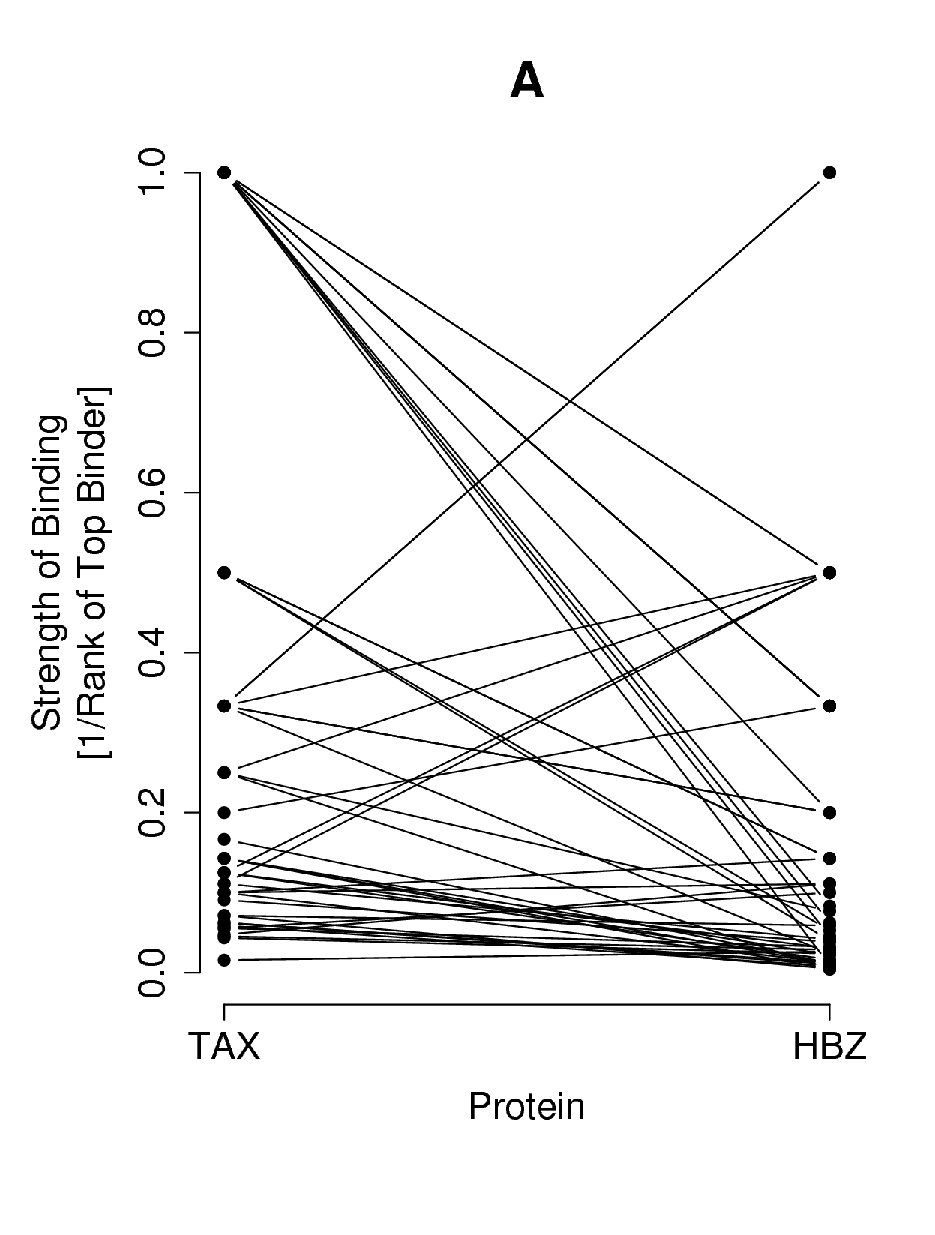
\includegraphics[width=7cm]{./Figures/chapter6/lower_res/immunogenicity_tax_hbz}%
\hspace{0cm}%
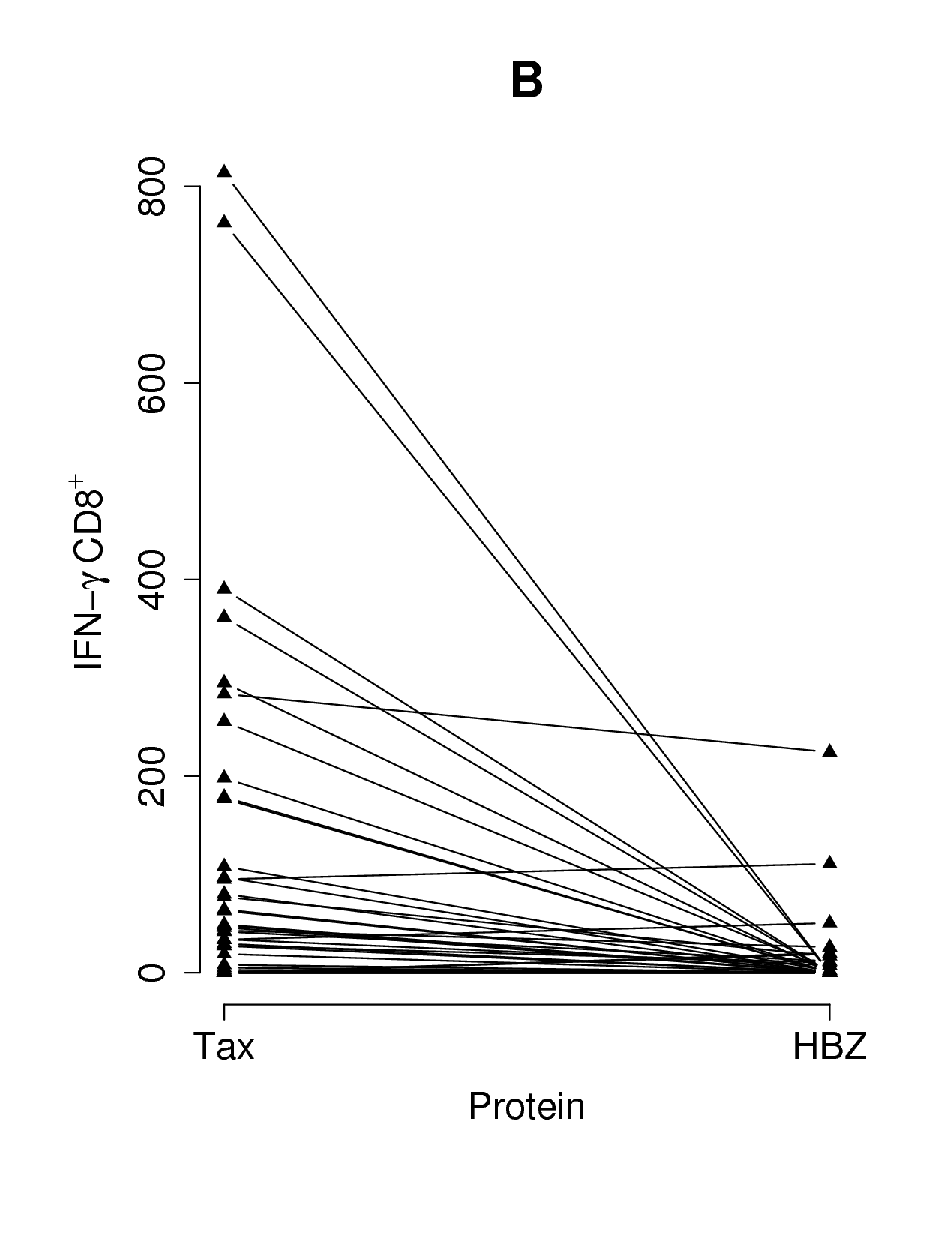
\includegraphics[width=7cm]{./Figures/chapter6/lower_res/immunogenicity_exper} \\
\caption[The comparative immunogenicity of HBZ and Tax]{The comparative immunogenicity of HBZ and Tax. A, The predicted top binding peptide from Tax and HBZ to each of the 43 alleles for which Metaserver predicts binding affinities was found. Peptides from Tax are bound more strongly than peptides from HBZ ($P = 0.00002$, paired Wilcoxon-Mann-Whitney). B, Consistent with this, the frequency of Tax-specific CD8$^+$ T cells was also greater compared to HBZ CD8$^+$ T cells in the 45 HTLV-I infected individuals tested using by IFN-$\gamma$ ELISpot ($P = 0.000006$, paired Wilcoxon-Mann-Whitney).}
\label{chapter6/figureImmun}
\end{figure}


%%%%%%%%%%%%%%%%%%%%%%%%%%%%%%%%%%%%%%%%%%%%%%%%%%%%%%%%%%%%%%%%%%%%%%%%%%%%%%%%%%%%%%%%%%%%%%%%%%%%

\begin{table}[htp]
\begin{center}

\begin{sideways}
{
\renewcommand{\arraystretch}{1.5}
\begin{tabulary}{1.5\textwidth}{|c|L|c|c|c|c|L|}
\hline
& \multirow{2}{*}{Null hypothesis} & \multicolumn{2}{c}{Rank measure} & \multicolumn{2}{|c|}{Raw score} & \multirow{2}{*}{Conclusion} \\
\cline{3-6}
& & Metaserver & Epipred & Metaserver & Epipred & \\	
\hline
1 & Protective and detrimental alleles target HBZ equally & \multicolumn{2}{c|}{$0.0002$} & - & - & Protective alleles bind HBZ significantly more strongly than detrimental alleles \\
\hline
2 & AC and HAM/TSP patients target HBZ equally & $0.0002$ & $0.000002$ & $0.002$ & $0.001$ & ACs have HLA alleles that bind HBZ significantly more strongly compared to HAM/TSP patients \\
\hline
3 & AC and HAM/TSP patients target HBZ equally (excluding A02, B54 and Cw08) & $0.04$ & $0.006$ & $0.14$ & $0.03$ & ACs bind HBZ significantly more strongly compared to HAM/TSP patients even when known protective and detrimental alleles are excluded \\
\hline
4 & There is no correlation between proviral load and the number of alleles that bind HBZ strongly & $0.016$ & $0.1$ & $0.01$ & $0.032$ & The higher the number of strong binding alleles to HBZ per individual, the lower their proviral load \\
\hline
5 & There is no correlation between proviral load and the strength of HBZ binding & $0.008$ & $0.04$ & $0.003$ & $0.085$ & The greater the strength of HBZ binding (rank method), the lower the proviral load \\
\hline
6 & There is no correlation between load reduction (count) and disease prevalence reduction & $0.0005$ & $0.02$ & $0.004$ & $0.03$ & Proteins that are strongly bound by asymptomatic carriers are, independently, those associated with a greater reduction in load when bound \\
\hline
7 & There is no correlation between load reduction (rank) and disease prevalence reduction & $< 2.2 \times 10^{-16}$ & $0.003$ & $0.002$ & $0.2$ & As above, using the rank measure to quantify the effect of binding strength on proviral load \\
\hline
\end{tabulary}
}
\end{sideways}
\end{center}

\caption[The summary of epitope prediction hypothesis testing]{The results of hypothesis testing repeated using different epitope prediction methods (Metaserver and Epipred) and different metrics (a rank measure which only compares within alleles (i.e. not between alleles) and a raw binding score measure which compares between as well as within alleles).}
\label{chapter6/table5}
\end{table}


%%%%%%%%%%%%%%%%%%%%%%%%%%%%%%%%%%%%%%%%%%%%%%%%%%%%%%%%%%%%%%%%%%%%%%%%%%%%%%%%%%%%%%%%%%%%%%%%%%%%
%%%%%%%%%%%%%%%%%%%%%%%%%%%%%%%%%%%%%%%%%%%%%%%%%%%%%%%%%%%%%%%%%%%%%%%%%%%%%%%%%%%%%%%%%%%%%%%%%%%%


\section{Discussion}\label{chapter6/discussion}

Using validated epitope prediction software, we show that strong binding of peptides from the HTLV-I basic leucine zipper factor (HBZ) protein is associated with a reduced risk of HAM/TSP and a reduced proviral load in a population with endemic HTLV-I infection in southern Japan. We demonstrated that protection is not limited to a small subset of HLA class I alleles previously associated with disease status and proviral load (HLA-A*02 and HLA-Cw*08), but is more generally associated with HLA class I alleles that bind strongly to HBZ.

Prior to this analysis CD8$^+$ T cells specific for the HTLV-I protein Tax were often considered as the best candidate for `efficient' or `protective' CD8$^+$ cells because of the immunodominance of Tax in the CD8$^+$ T cell response \citep{Kannagi1991, Goon2004}. Our finding that binding of HBZ peptides rather than Tax peptides is protective raises the question why HBZ? 

The HBZ gene was identified recently \citep{Gaudray2002}. It is encoded by the complementary strand of the HTLV-I genome and its promoter lies in the 3� LTR rather than the 5� LTR. It functions by binding to the transcription factor CREB-2. There are two major splice variants of the HBZ transcript, SP1 and SP2; the variant SP1 is more abundant and is the variant used in this study \citep{Cavanagh2006}. Expression of HBZ suppresses Tax-mediated transactivation through the 5� LTR \citep{Gaudray2002, Basbous2003} and thereby inhibits expression of other HTLV-I genes \citep{Gaudray2002, Li2009}; HBZ can be expressed in the absence of transcription of other HTLV-I genes. Additionally, HBZ RNA promotes the proliferation of infected T-lymphocytes \citep{Satou2006}. This dual action - reduction of HTLV-I expression and subsequent protection from immune surveillance, and enhancement of infected cell proliferation - probably confers a survival advantage on HBZ-expressing cells and is consistent with the observations that HBZ enhances persistence in HTLV-I inoculated rabbits \citep{Li2009} and that ATL cells often have a hypermethylated or deleted 5� LTR but an intact functional 3� LTR \citep{Satou2006}.

We hypothesise that if HBZ-specific CD8$^+$ T cells are weak or absent then infected cells that express HBZ but not other viral proteins will escape immune surveillance and proliferate rapidly, leading to a large increase in proviral load. HBZ-specific CD8$^+$ T cells would then play an important role in preventing this proliferation of provirus-positive cells and blocking this strategy of persistence. If this conclusion is correct that HLA class I recognition of HBZ plays a central role in the control of HTLV-I replication than one might expect that HBZ in HTLV-I would have evolved to minimize the effect of this class I recognition. Consistent with this hypothesis, we find that the predicted binding affinity to HBZ peptides is significantly weaker than that of Tax peptides and that the frequency of HBZ-specific CD8$^+$ T cells is significantly lower than the frequency of Tax-specific CD8$^+$ T cells. Although the low immunogenicity of HBZ is precisely what we predict given its central importance in maintaining HTLV-I persistence it is nevertheless striking that these low frequency responses are so important. This result challenges the prevailing assumption in HTLV-I research and in immunology in general that the immunodominant responses are the most interesting and important.

This approach to studying the association between HLA class I genotype and the outcome of infection has a number of strengths compared with a traditional frequency-based analysis. Firstly, it is more mechanistic: knowing that binding HBZ is associated with a reduced proviral load and disease risk compared with knowing that A*02 is associated with these outcomes is a simultaneously more fundamental and more applicable level of understanding. Secondly, identification of protective epitopes immediately suggests a practical approach to increase the efficiency of an individual�s anti-viral response. Thirdly, because the same effect (e.g.~HBZ binding) can be identified for many alleles it is less likely to be a spurious result of linkage disequilibrium or genetic stratification. Finally, effects due to multiple low-frequency alleles can be captured because analysis is made at the level of peptide binding rather than allelic frequency. 

In summary, using a novel and generalizable approach, we have identified one of the constituents of an effective CD8$^+$ T cell response in HTLV-I infection.

%%%%%%%%%%%%%%%%%%%%%%%%%%%%%%%%%%%%%%%%%%%%%%%%%%%%%%%%%%%%%%%%%%%%%%%%%%%%%%%%%%%%%%%%%%%%%%%%%%%%
%%%%%%%%%%%%%%%%%%%%%%%%%%%%%%%%%%%%%%%%%%%%%%%%%%%%%%%%%%%%%%%%%%%%%%%%%%%%%%%%%%%%%%%%%%%%%%%%%%%%	% Specificity
% Chapter 6, changed from chapter 5 - still labelled as chapter 5

\chapter{Antigen Expression as a Determinant of CTL Lysis in HTLV-I Infection} % Write in your own chapter title
\label{Chapter5}
\lhead{Chapter 6. \emph{Antigen Expression as a Determinant of CTL Lysis}}

\section{Introduction}

So far, this study has concentrated on the epitope properties that are associated with disease risk and proviral load. For this chapter, we extended this work to examine the CD8$^+$ T cell response itself, specifically in terms of its dynamics as a function of antigen expression of infected CD4$^+$ T cells. 

In human T-lymphotropic virus type 1 (HTLV-I) infection, a high frequency of HTLV-I-specific CTLs can co-exist stably with a high
proviral load and the proviral load is strongly correlated with the risk of HTLV-I-associated inflammatory diseases. In \cref{Chapter2}, \sref{chapter2/CTLResponse}, it was discussed how these observations have led to the hypothesis that HTLV-I specific CTLs are ineffective in controlling HTLV-I replication but contribute to the pathogenesis of the inflammatory diseases. However, evidence from host and viral immunogenetics and gene expression microarrays suggests that a strong CTL response is associated with a low proviral load and a low risk of HAM/TSP. To further examine the role of CTLs in HTLV-I infection, a collaborative experiment was carried out to quantify the frequency, lytic activity and functional avidity of HTLV-I-specific CD8$^+$ cells in fresh, unstimulated PBMCs from individuals with natural HTLV-I infection. The ELISpot assays and flow cytometry experiments were performed by Aileen Rowan and Tarek Kattan. My role, using a system of ordinary differential equations, was to quantify the efficiency of CD8$^+$ lysis in their \emph{ex vivo} experiments.   

We have previously investigated methods of quantifying antiviral CTL efficiency. In HTLV-I infection, both effector CTLs and infected target cells are often present in fresh blood at frequencies sufficiently high to obviate the need for enrichment of specific
subpopulations. We have exploited this feature to develop an assay of CD8$^+$ cell-mediated suppression of HTLV-I expression in
fresh PBMCs \citep{Asquith2005a}. As a marker of proviral expression we use the viral protein Tax, a regulatory protein expressed early in the life cycle of HTLV-I \citep{Asquith2005a}. We previously showed that this suppression of HTLV-I depended on CD8$^+$ T cell frequency and required both perforin and a match in class 1 MHC genotype between effector and target cells \citep{Hanon2000}, consistent with classical class 1 MHC-restricted CTL lysis. Mathematical modeling can be used to quantify the rate of killing of Tax-expressing CD4$^+$ cells per CD8$^+$ cell per day. We use the term lytic efficiency to denote this per-CD8$^+$-cell rate of lysis. This assay of lytic efficiency showed that the rate of CTL-mediated lysis of HTLV-I-infected cells in fresh PBMCs was inversely correlated with the proviral load, both in patients with HAM/TSP and in asymptomatic HTLV-I carriers (ACs) \citep{Asquith2005a}.

This measure of lytic efficiency has two chief limitations. First, the antiviral activity is expressed per CD8$^+$ cell, not per virus-specific CD8$^+$ cell, since there is no currently available method to measure in the same assay the lytic activity and the total frequency of CD8$^+$ T cells specific to all viral epitopes in each individual (an ELISpot assay that detects IFN$\gamma$ production comes closest to this definition. However, this assay only detects the activation of CD8$^+$ cells and not their lytic efficiency). Second, rate of lysis is likely to be a composite parameter that is a function of both the frequency of the Ag specific CD8$^+$ cells and the ``quality'' of their effector functions at the single-cell level \citep{Seder2008} (i.e.~it is not clear what effector functions might affect the lysis rate). In an acute viral infection, efficient elimination of the virus is associated with a high frequency of Ag-specific T cells \citep{Stambas2007}. But in persistent infections, the complexity of the equilibrium dynamics makes it impossible to infer the efficiency of virus-specific CTLs directly from their steady-state frequency \citep{Asquith2007}.

For this chapter, I modified this model of lytic efficiency to take account of the observation that Tax expression per cell is not constant in the HTLV-I-infected target CD4$^+$ cells, but increases over the 18 hour incubation time. The results of this analysis were estimates of the lytic efficiency of CTLs specific to high Tax expressing cells and, separately, low Tax expressing cells.

%%%%%%%%%%%%%%%%%%%%%%%%%%%%%%%%%%%%%%%%%%%%%%%%%%%%%%%%%%%%%%%%%%%%%%%%%%%%%%%%%%%%%%%%%%%%%%%%%%%%

\section{Methods}

The cell preparation, culture and flow cytometry analysis was carried out by Tarek Kattan.

\subsection{PBMC Separation}

Peripheral blood mononuclear cells (PBMCs) were isolated from whole blood by density gradient centrifugation using Histopaque-1077 (Sigma, Poole, United Kingdom) from EDTA-anticoagulated blood samples taken from HTLV-I infected individuals. All individuals attended the HTLV-I clinic at St Mary�s Hospital, London and gave written informed consent. Isolated PBMCs were washed twice in PBS and then cryopreserved in fetal calf serum (FCS, Sigma) with 10\% dimethyl sulfoxide (DMSO, Sigma).

\subsection{Cell Culture}\label{chapter5/methodsCulture}

Cells were thawed, washed twice in PBS and then cultured in complete medium consisting of RPMI 1640 medium (Sigma) supplemented with
10\% FCS, 2 mM L-Glutamine, 100 U/ml Penicillin and 100$\mu$g/ml Streptomycin (Life Technologies). Cells were incubated for different times at $37\,^{\circ}\mathrm{C}$ in 5\% CO$_2$. When required, CD8$^+$ or CD4$^+$ cells were depleted by positive selection using Ab coated magnetic microbeads following the manufacturer's instructions (Miltenyi Biotec, Surrey, United Kingdom).

\subsection{Flow Cytometric Detection of Tax Expression}

After incubation, cells were surface-stained with mAbs specific to CD4 and CD8 at 15$\mu$g/ml in each case (Beckman Coulter, Marseille, France). Cells were fixed with 2\% paraformaldehyde (PFA, Sigma) and then permeabilized using PBS/0.1\% Triton X-100 (Sigma). Finally, cells were stained intracellularly with the FITC conjugated Ab anti-Tax protein Lt-4 \citep{Lee1989}, diluted 1/100. Cells were analyzed on a Coulter Epics XL flow cytometer. Thirty thousand events were routinely collected during acquisition of the data. The data were analyzed using Coulter Expo32 software (Beckman Coulter). Tax$^+$cells were divided in flow-cytometric analysis into two gates, corresponding respectively to Tax\superscript{low} and Tax\superscript{high} cells according to fluorescence intensity. The line dividing these gates was arbitrarily defined; the same definition was used in the analysis of all samples.

\subsection{Rate of CD8$^+$ Cell-mediated Lysis}\label{chapter5/methodsLysis}

The rate (``efficiency'') of CD8$^+$ cell-mediated lysis of HTLV-I-infected cells was estimated as previously described \citep{Asquith2005a}. CD8$^+$ cell lytic efficiency (expressed as the proportion of Tax-expressing CD4$^+$ cells killed per CD8$^+$ cell per day) was calculated for each HTLV-I-infected individual tested using \eref{chapter5/equation1}:

\begin{equation}
\frac{dy}{dt} = c - \epsilon y z
\label{chapter5/equation1}
\end{equation}

where $y$ is the proportion of CD4$^+$ cells expressing Tax, $c$ is the rate of increase of Tax expression, which is assumed to be constant during the short-term culture, $\epsilon$ is the CD8$^+$ cell-mediated antiviral efficacy (expressed as the proportion of CD4$^+$ Tax$^+$ cells killed per CD8$^+$ cell per day) and $z$ is the proportion of lymphocytes that are CD8$^+$. This model was solved analytically and fitted to the data using non-linear least-squares regression (SPSS v12), providing an estimate of the antiviral efficacy ($\epsilon$) in each individual.

\eref{chapter5/equation1} used a constant rate $c$ to describe Tax expression in the absence of CD8$^+$ cells. However, since observations from experimental time course data (\fref{chapter5/figureTimeCourse}) suggested a non-linear rate of increase of Tax expression, it was necessary to modify the existing model. 2 models were considered as possibilities:

\begin{center}

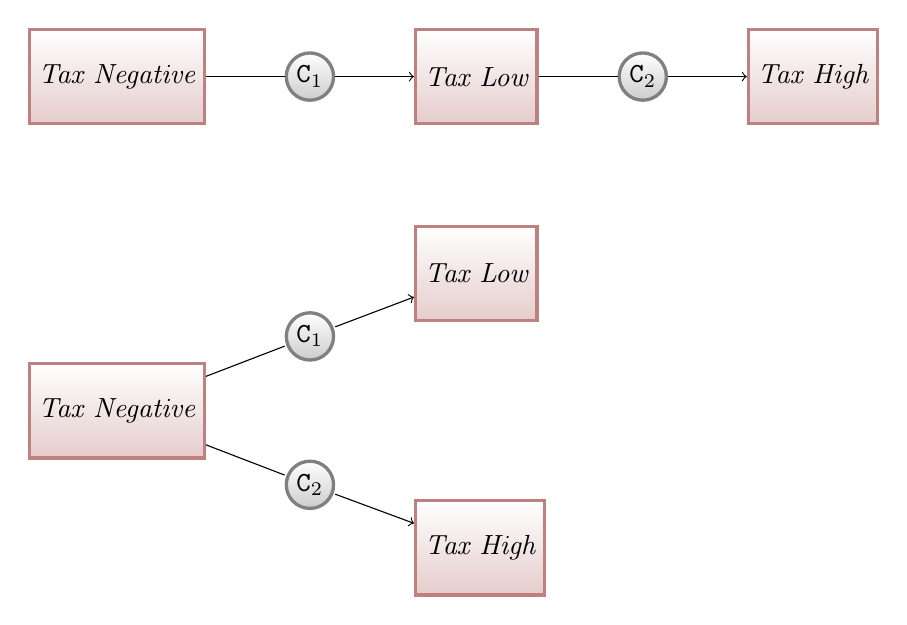
\begin{tikzpicture}[nonterminal/.style={
	rectangle,
	minimum size=12mm,
	very thick,
	draw=red!50!black!50, 
	top color=white, 
	bottom color=red!50!black!20,
	font=\itshape
	},terminal/.style={
	rectangle,minimum size=6mm,rounded corners=3mm,
	very thick,draw=black!50,
	top color=white,bottom color=black!20,
	font=\ttfamily
	}
]

\node (atom1) [nonterminal] {Tax Negative};
\node (rate1) [terminal,right=of atom1] {C$_1$};
\node (atom2) [nonterminal,right=of rate1] {Tax Low};
\node (rate2) [terminal,right=of atom2] {C$_2$};
\node (atom3) [nonterminal,right=of rate2] {Tax High};

\path	(atom1) edge[-] (rate1)
	(rate1) edge[->] (atom2)
	(atom2) edge[-] (rate2)
	(rate2) edge[->] (atom3);

\node (atom4) [nonterminal, below=of atom1, yshift=-20mm] {Tax Negative};
\node (rate3) [terminal, above right=of atom4, yshift=-10mm] {C$_1$};
\node (rate4) [terminal, below right=of atom4, yshift=10mm] {C$_2$};
\node (atom5) [nonterminal, right=of rate3, yshift=8mm] {Tax Low};
\node (atom6) [nonterminal, right=of rate4, yshift=-8mm] {Tax High};

\path	(atom4) edge[-] (rate3)
	(rate3) edge[->] (atom5)
	(atom4) edge[-] (rate4)
	(rate4) edge[->] (atom6);

\end{tikzpicture}
\end{center}

The first model represents a progression from Tax\superscript{negative} to Tax\superscript{low} to Tax\superscript{high} expressing CD4$^+$ cells as a single population. The second models the appearance of Tax\superscript{low} and Tax\superscript{high} expressing CD4$^+$ cells as 2 distinct populations. Instead of a single parameter $c$ that defines the rate of increase of Tax expression in \eref{chapter5/equation1}, each model introduces 2 rate parameters: $c_1$, the rate of increase of low Tax expression and $c_2$, the rate of increase of high Tax expression. Both models were fitted to the time course data and it was found that the `single population' model was a more accurate fit of the data (see \sref{chapter5/results/TaxExpress}). The `single population' model was designated `Model 1'.

In Model 1, the Tax\superscript{low} population (as defined from the gated FACS) is produced at a constant rate $c_1$ and the Tax\superscript{high} population at a rate $c_2$. The following pair of linked ordinary differential equations, \eref{chapter5/equation2} and \eref{chapter5/equation3}, describe the model:

\begin{equation}
\frac{dy}{dt} = c_1 - c_2y
\label{chapter5/equation2}
\end{equation}

\begin{equation}
\frac{dw}{dt} = c_{2}y
\label{chapter5/equation3}
\end{equation}

Here, $y$ is the proportion of CD4$^+$ cells expressing low levels of Tax and $w$ is the proportion of CD4$^+$ cells expressing high levels of Tax. Solving these equations, we have \eref{chapter5/equation4} and \eref{chapter5/equation5}:

\begin{equation}
y = \left( \frac{c_1}{c_2} \right) \left( 1 - e^{-c_2 t} \right)
\label{chapter5/equation4}
\end{equation}

\begin{equation}
w = c_1 \left( t + \frac{e^{-c_2 t}}{c_2} - \frac{1}{c_2} \right)
\label{chapter5/equation5}
\end{equation}

\eref{chapter5/equation4} and \eref{chapter5/equation5} were fitted to the data using non-linear least-squares regression (\tref{chapter5/table1}), providing an estimate for $c_1$ and $c_2$ in each individual. \eref{chapter5/equation2} and \eref{chapter5/equation3} were then modified to describe the rate of CD8$^+$ cell-mediated lysis of Tax\superscript{low} CD4$^+$ cells and Tax\superscript{high} CD4$^+$ cells separately:

\begin{equation}
\frac{dy}{dt} = c_1 - c_2 y - \epsilon^{\text{low}} y z 
\label{chapter5/equation6}
\end{equation}

\begin{equation}
\frac{dw}{dt} = c_1\left(1 - \frac{1}{e^{c_2t}}\right) - \epsilon^{\text{high}} w z 
\label{chapter5/equation7}
\end{equation}

\eref{chapter5/equation6} and \eref{chapter5/equation7} (Model 2) were solved analytically and fitted to the data using non-linear least-squares regression. From the resulting data, estimates for the rate of killing of CD4$^+$ cells expressing low levels of Tax ($\epsilon$\superscript{low}) and high levels of Tax ($\epsilon$\superscript{high}) were produced for each individual.

\subsubsection{Bootstrap}\label{chapter5/methodsBootstrap}

A bootstapping method was used to test the robustness of the $\epsilon$\superscript{low} and $\epsilon$\superscript{high} parameters for each patient. 50 new datasets were generated per individual for both their expression levels of Tax\superscript{low} and Tax\superscript{high}. \eref{chapter5/equation6} and \eref{chapter5/equation7} were then fitted to this data, which gave a standard deviation of the resulting values of $\epsilon$\superscript{low} and $\epsilon$\superscript{high} (see \tref{chapter5/table1}).

%%%%%%%%%%%%%%%%%%%%%%%%%%%%%%%%%%%%%%%%%%%%%%%%%%%%%%%%%%%%%%%%%%%%%%%%%%%%%%%%%%%%%%%%%%%%%%%%%%%%

\section{Results}

\subsection{Modeling Tax expression}\label{chapter5/results/TaxExpress}

Flow cytometric analysis was used to divide the Tax-expressing CD4$^+$ population into high Tax-expressing and low Tax-expressing
cells. The 2 models of Tax expression, `single' and `dual' populations, were solved and fitted to the experimental data to give estimates of the parameters $c_1$ and $c_2$ in each case. \tref{chapter5/tableTaxFits} shows the $R^2$ values for the fits of the respective models for each of the patients. The accuracy of the `single population' model was significantly better for low Tax expression and better for high Tax expression (Tax low: $P = 0.0001$, Tax high, $P = 0.095$; paired Wilcoxon-Mann-Whitney). From these results, we chose the `single population' as our model of Tax expression over 18 hours.

\begin{table}[htp]
\begin{center}

\begin{tabular}{|c|c|c|c|c|c|}
\hline
& Names & Single Low & Single High & Dual Low & Dual High \bigstrut \\
\hline
1 & HAP  & 0.4571 & 0.8297 & 0.1126 & 0.8575 \bigstrut[t] \\
2 & HAY  & 0.8710 & 0.8408 & 0.8586 & 0.1214 \\
3 & HBE  & 0.2665 & 0.4938 & -0.2782 & 0.4277 \\
4 & HBX  & 0.7376 & -1.4986 & 0.6609 & 0.2523 \\
6 & HCH  & 0.1675 & 0.4303 & -0.2767 & 0.7503 \\
8 & HFB  & -1.0925 & 0.7753 & -2.6407 & 0.7978 \\
11 &  TAK & 0.8165 & 0.4660 & 0.8179 & 0.0435 \\
12 &  TAQ & 0.9461 & 0.8541 & 0.9361 & 0.7629 \\
13 &  TAW & -0.0586 & -0.2140 & -0.5068 & 0.4870 \\
14 &  TAZ & 0.8401 & 0.7504 & 0.8006 & 0.0256 \\
15 &  TBC & 0.6124 & 0.9268 & -0.2076 & -0.7341 \\
16 &  TBJ & 0.7501 & 0.6986 & 0.5346 & -0.0517 \\
17 &  TBP & 0.7397 & 0.9457 & 0.3094 & -0.1896 \\
19 &  TCL & 0.6367 & 0.5781 & 0.3577 & 0.1122 \\
20 &  UV1 & -0.1119 & 0.6705 & -0.7201 & -1.6188 \bigstrut[b] \\
\hline
\end{tabular}
\end{center}

\caption[The accuaracy of alternative models of Tax expression]{The $R^2$ values showing the accuracy of the single and dual population models fitting the experimental time course data of Tax\superscript{low} and Tax\superscript{high} expression.}
\label{chapter5/tableTaxFits}
\end{table}

\eref{chapter5/equation2} and \eref{chapter5/equation3} were then fitted to the Tax\superscript{low} and Tax\superscript{high} data respectively by non-linear least squares regression. Values for the parameters $c_1$ and $c_2$ were calculated from this analysis for each of the 15 patients (\tref{chapter5/table1}). Examples for 6 of the patients are shown in \fref{chapter5/figureTimeCourse}. The data for the other 9 patients is in \aref{AppendixB}, \fref{appendixb/figureTimecourse}.


\begin{figure}[htp]
\centering
\includegraphics[width=7cm]{./Figures/chapter5/figure_timecourse_hap}%
\hspace{0cm}%
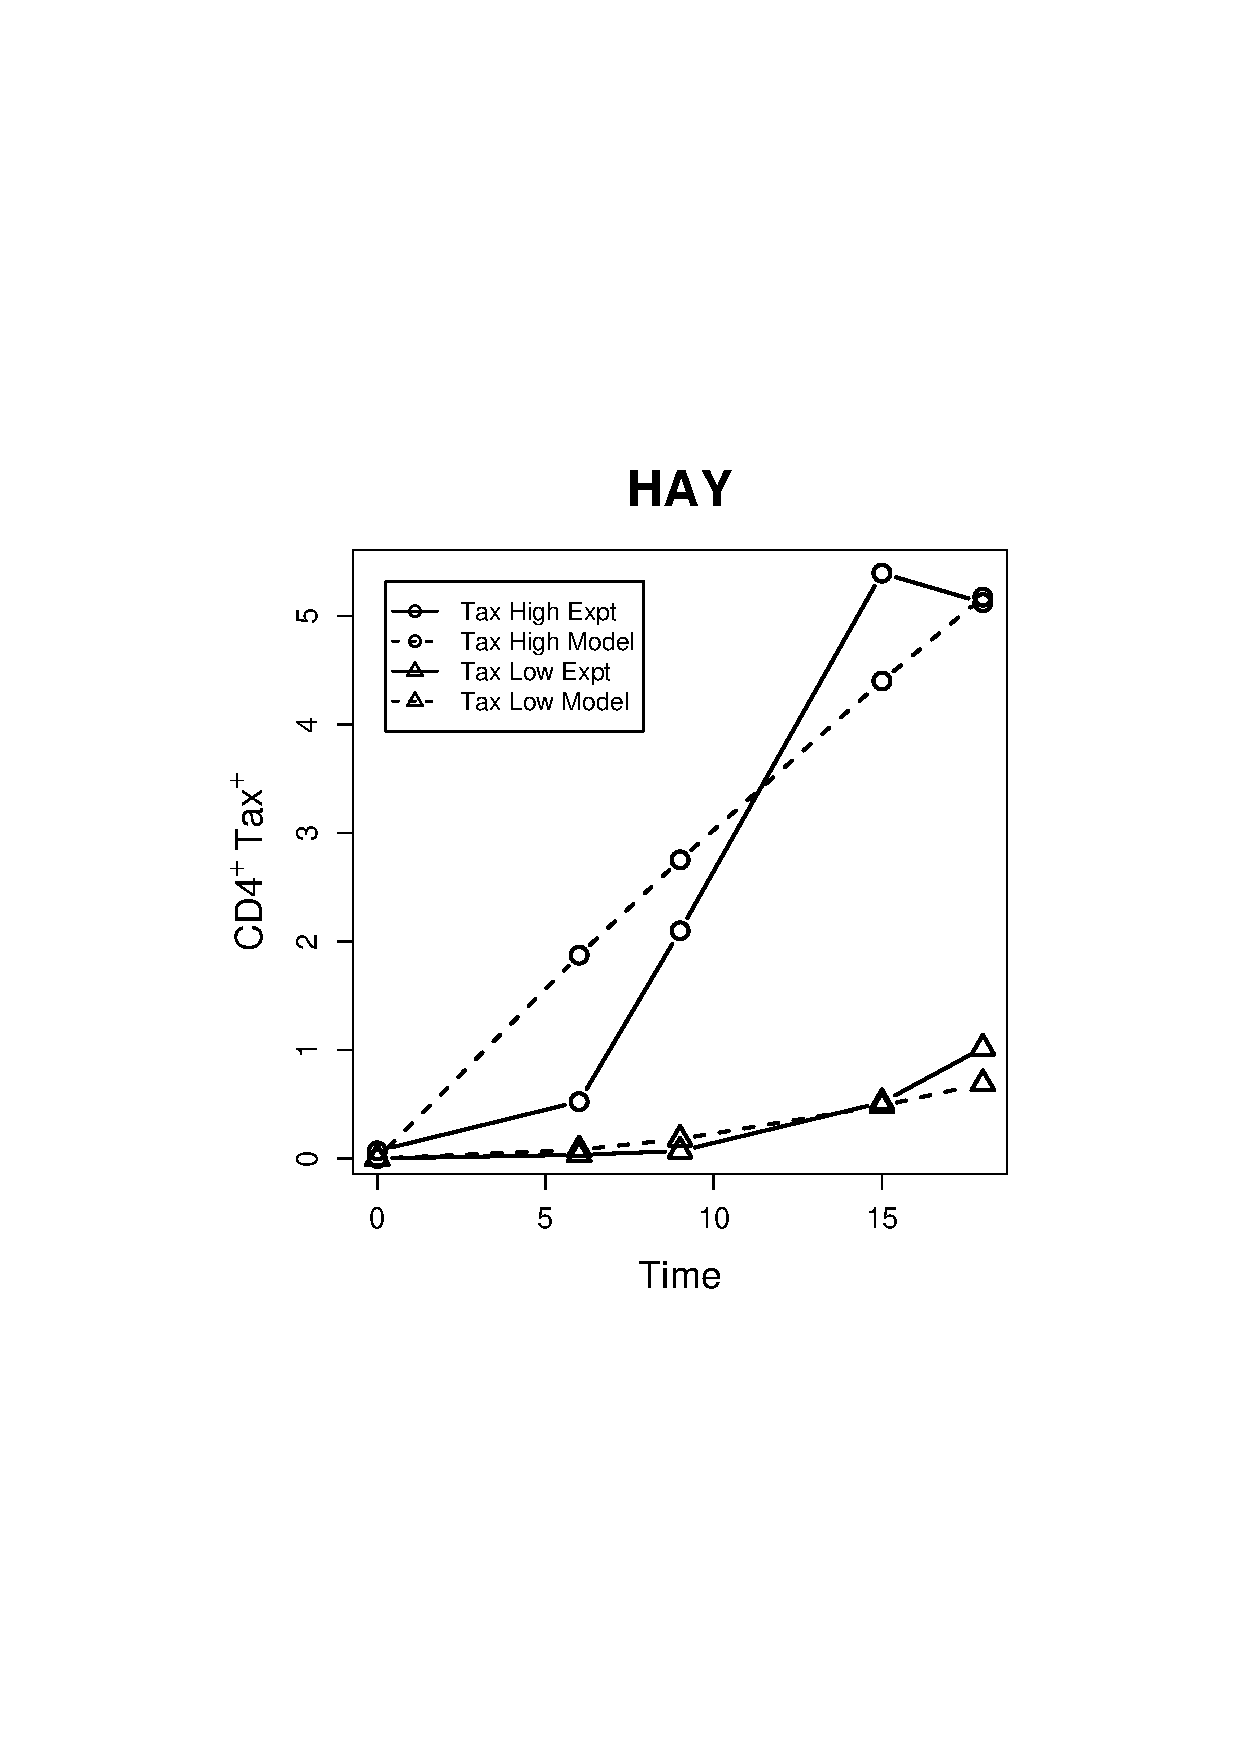
\includegraphics[width=7cm]{./Figures/chapter5/figure_timecourse_hay} \\
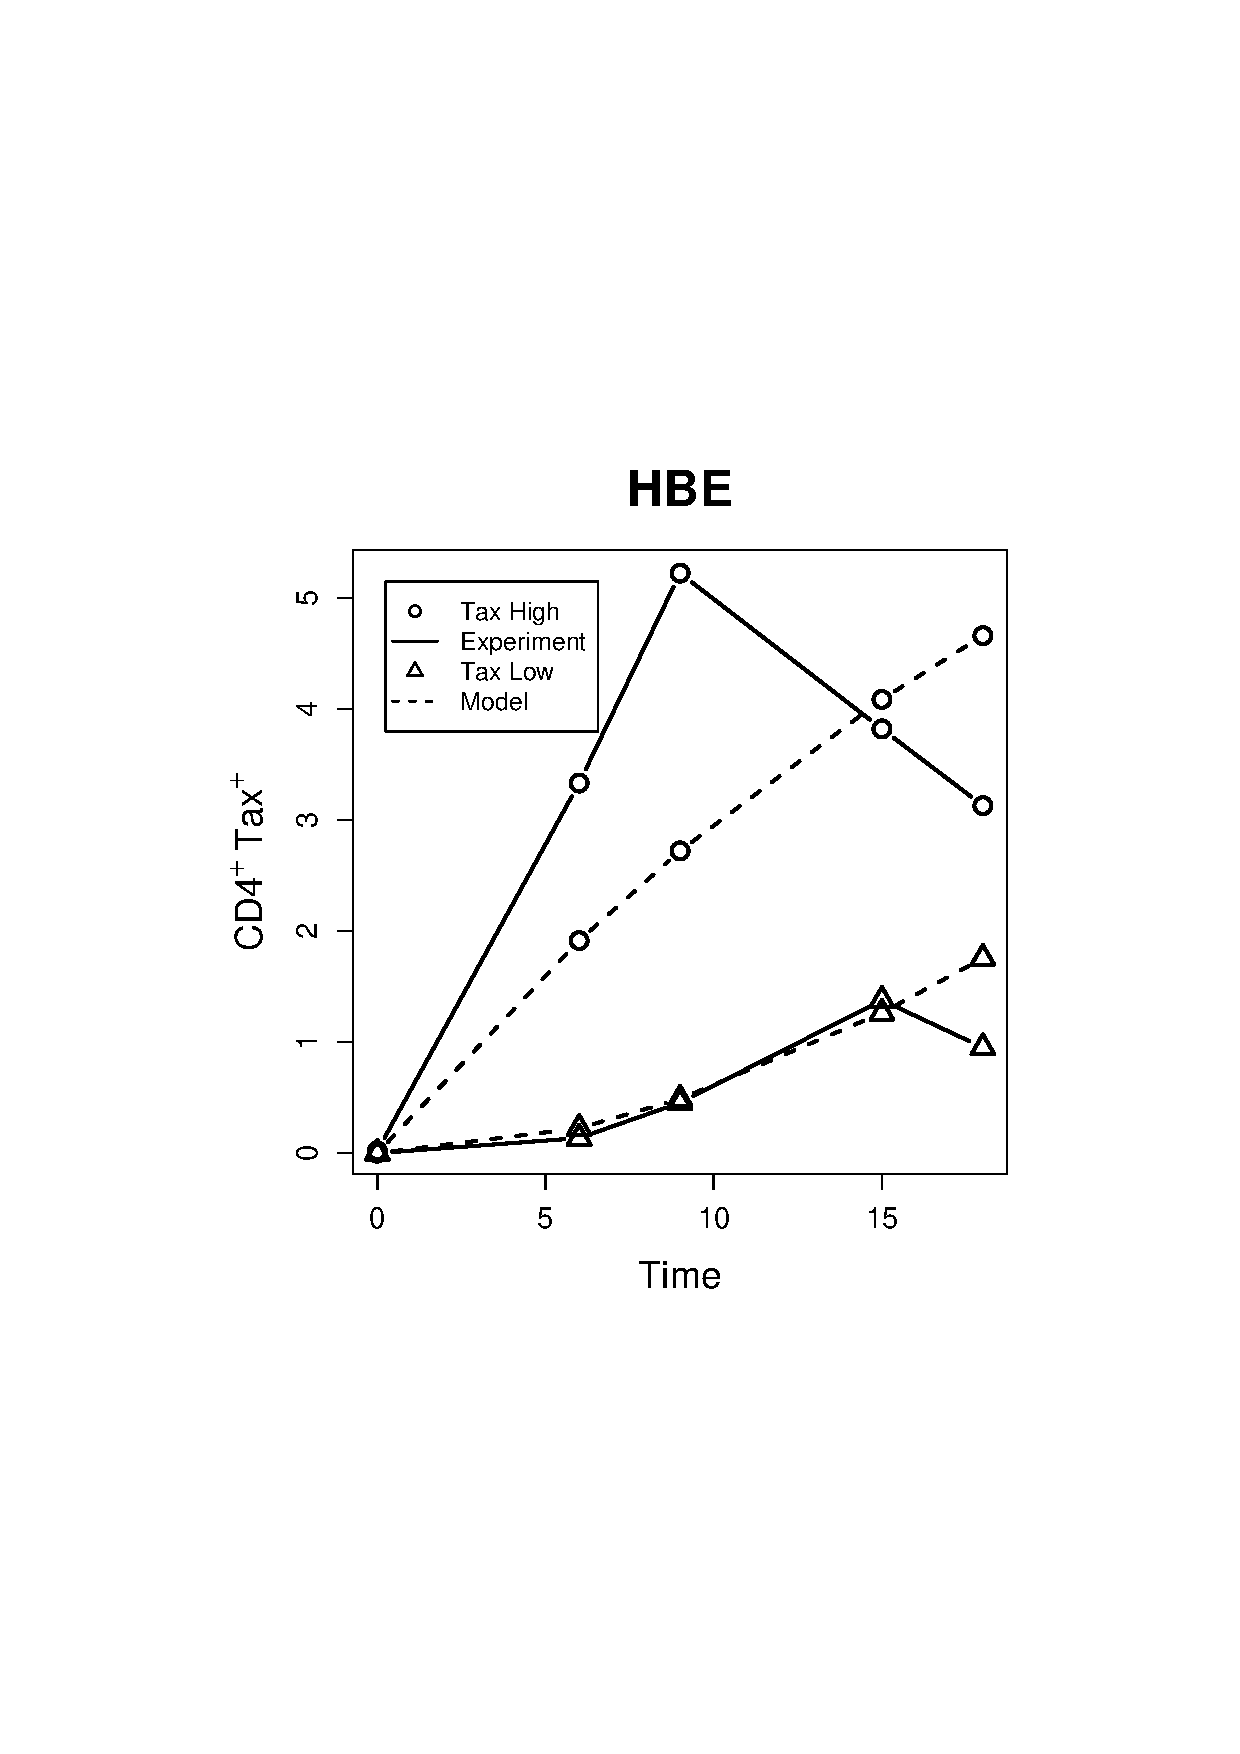
\includegraphics[width=7cm]{./Figures/chapter5/figure_timecourse_hbe}%
\hspace{0cm}%
\includegraphics[width=7cm]{./Figures/chapter5/figure_timecourse_hbx} \\
\includegraphics[width=7cm]{./Figures/chapter5/figure_timecourse_hch}%
\hspace{0cm}%
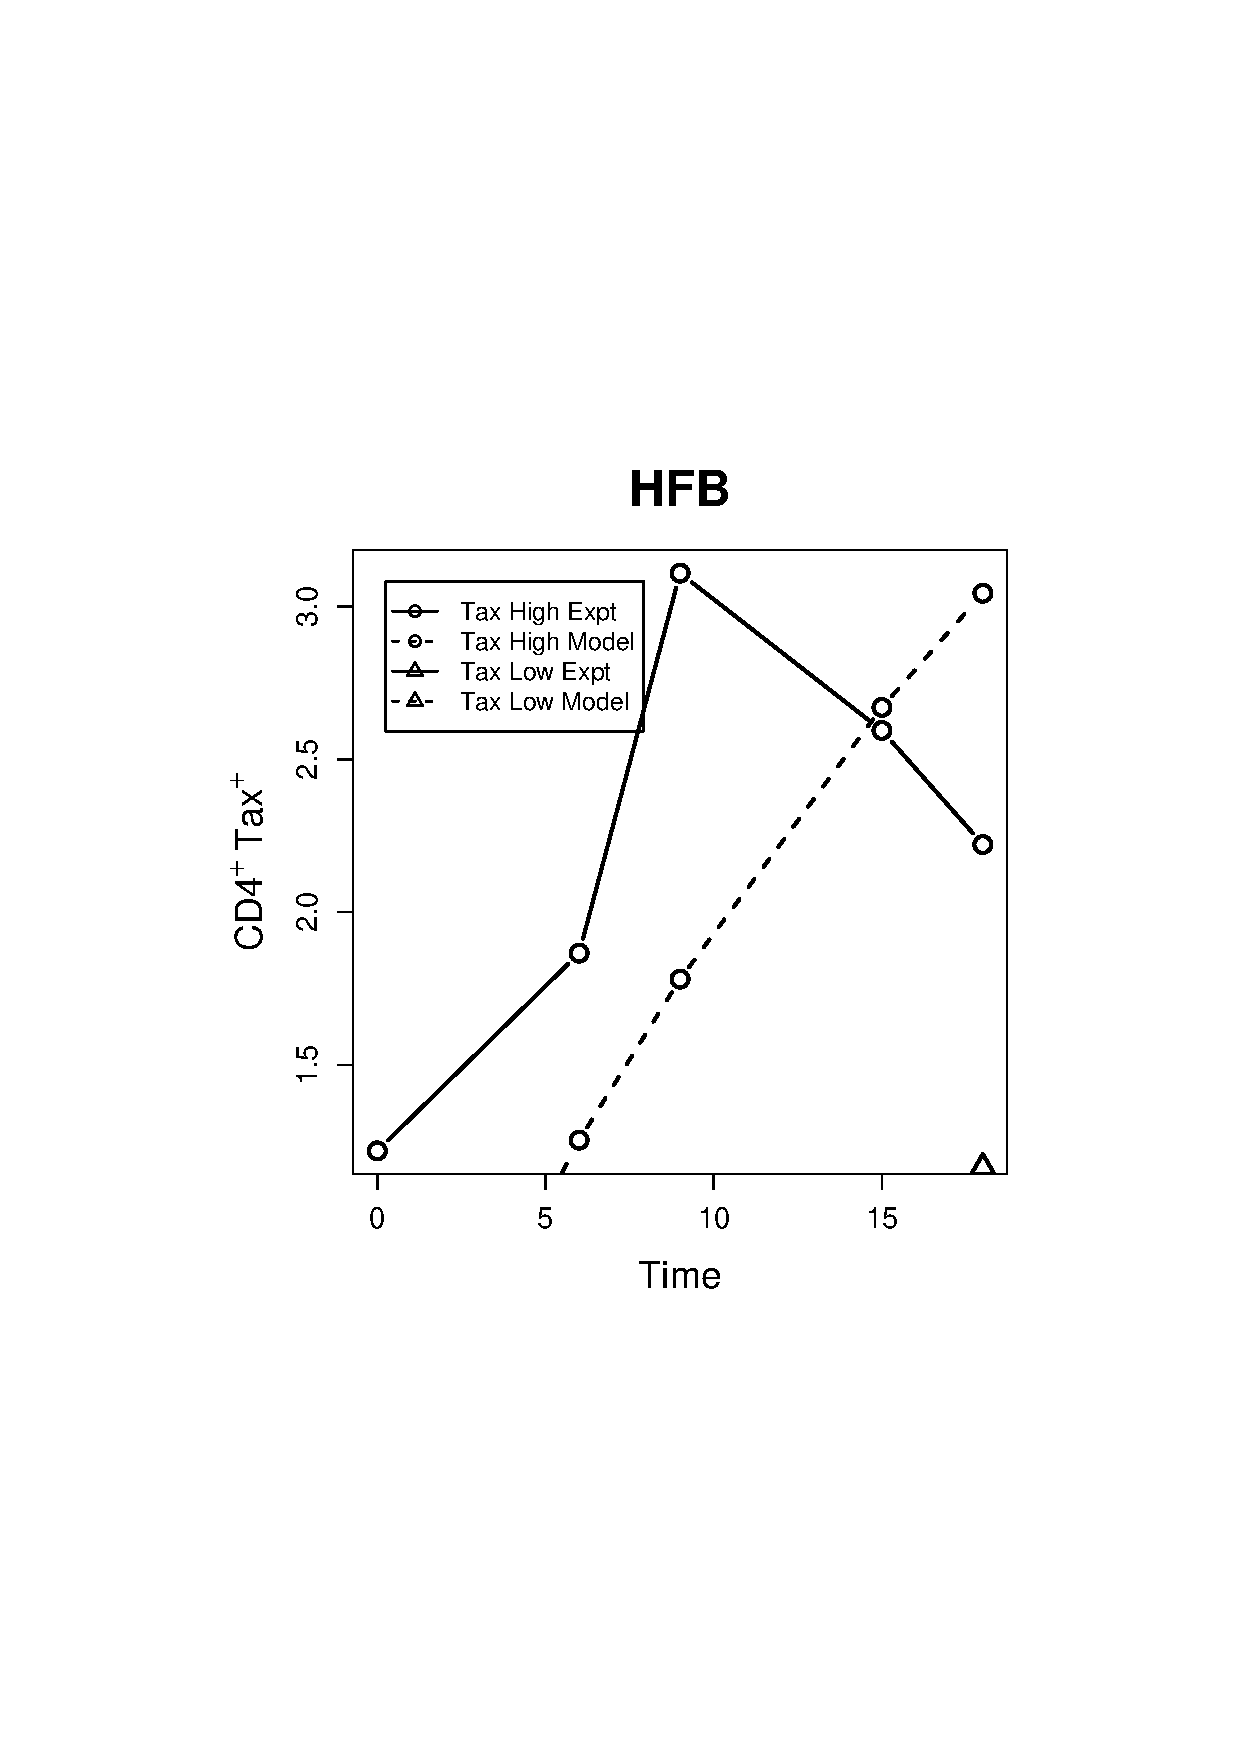
\includegraphics[width=7cm]{./Figures/chapter5/figure_timecourse_hfb} \\
\caption[The Tax expression time course]{This figure shows examples of the time course of Tax expression as the proportion of CD4$^+$ lymphocytes that were Tax\superscript{high} or Tax\superscript{low} over 18 hours culture (see \sref{chapter5/methodsCulture}). \eref{chapter5/equation2} and \eref{chapter5/equation3} were fitted to the Tax\superscript{low} and Tax\superscript{high} data respectively.}
\label{chapter5/figureTimeCourse}
\end{figure}

\subsection{The CD8$^+$ Antiviral Efficacy Assay}

\eref{chapter5/equation6} and \eref{chapter5/equation7} were fitted to the antiviral efficacy assay data for all 15 patients. The data shown for each patient is the proportion of CD4$^+$ lymphocytes that were Tax\superscript{high} and Tax\superscript{low} following 18 h co-culture with different proportions of CD8$^+$ lymphocytes. The parameters $\epsilon$\superscript{low} and $\epsilon$\superscript{high} were measured by non-linear least squares regression. The assay was repeated in each patient. \fref{chapter5/figureLysisAssay} shows this data for 3 patients. The data for the other 12 patients is in \aref{AppendixB}, \fref{appendixb/figureLysisHighLow}.

\fref{chapter5/figurePairedEpsilon} shows a statistically significantly higher rate of CD8$^+$ cell-mediated lysis of the Tax\superscript{high} cells than that of the Tax\superscript{low} cells ($P = 0.004$, Wilcoxon-Mann-Whitney, $n=15$). \fref{chapter5/figureCompareLysis} shows the plot of $\epsilon$\superscript{low} against $\epsilon$\superscript{high} for each patient. The strong linear relationship ($R^2 = 0.855$, $P < 0.001$) suggests the ratio $\epsilon$\superscript{high}/$\epsilon$\superscript{low} is maintained across patients.

There was strong agreememt between the 2 repeats per patients of the estimates for $\epsilon$\superscript{low} and $\epsilon$\superscript{high} ($\epsilon$\superscript{low}: $R^2 = 0.9492$, $P < 0.001$. $\epsilon$\superscript{high}: $R^2 = 0.890$, $P < 0.001$; \aref{AppendixB}, \fref{appendixb/figureLysisHighLow}). \aref{AppendixB} also contains a comparison of the original $\epsilon$ and $c$ parameters from \eref{chapter5/equation1} against $\epsilon$\superscript{low} and $\epsilon$\superscript{high} (\fref{appendixb/figure2}) and $c_1$ and $c_2$ (\fref{appendixb/figure3}).

Finally, \aref{AppendixB}, \fref{chapter5/figureRatio} shows there was no difference in the ratio of Tax expression between HAM/TSP patients and ACs ($P = 0.871$, Wilcoxon-Mann-Whitney, HAM/TSP: $n=16$, AC: $n=12$).

\begin{figure}[htp]
\centering
\includegraphics[width=7cm]{./Figures/chapter5/figure_lysis_hap_rep_1}%
\hspace{0cm}%
\includegraphics[width=7cm]{./Figures/chapter5/figure_lysis_hap_rep_2} \\
\includegraphics[width=7cm]{./Figures/chapter5/figure_lysis_hay_rep_1}%
\hspace{0cm}%
\includegraphics[width=7cm]{./Figures/chapter5/figure_lysis_hay_rep_2} \\
\includegraphics[width=7cm]{./Figures/chapter5/figure_lysis_hbe_rep_1}%
\hspace{0cm}%
\includegraphics[width=7cm]{./Figures/chapter5/figure_lysis_hbe_rep_2} \\
\caption[CD8$^+$ antiviral efficacy assay]{The figure
shows examples of the antiviral efficacy assay for patients HAP, HAY and HBE. The proportion of CD4$^+$ lymphocytes that were Tax\superscript{high} and Tax\superscript{low} following 18 h co-culture with different proportions of CD8$^+$ lymphocytes was measured. The model (\eref{chapter5/equation6} and \eref{chapter5/equation7}, \sref{chapter5/methodsLysis}) was fitted to this data and in this way the rate of clearance of Tax\superscript{low}CD4$^+$ and Tax\superscript{high}CD4$^+$ cells per day per CD8$^+$ cell (antiviral efficacy) was estimated. This was repeated in the same subject.}
\label{chapter5/figureLysisAssay}
\end{figure}

\begin{figure}[htp]
\centering
\includegraphics[width=14cm]{./Figures/chapter5/pairedEpsilon}
\caption[A paired comparison of the rates of lysis]{The rates of lysis $\epsilon$\superscript{low} and $\epsilon$\superscript{high} compared per patient. Tax\superscript{high} cells were killed faster than Tax\superscript{low} cells in the same individual ($P = 0.004$, Wilcoxon-Mann-Whitney, $n=15$).}
\label{chapter5/figurePairedEpsilon}
\end{figure}

\begin{figure}[htp]
\centering
\includegraphics[width=14cm]{./Figures/chapter5/figureEpsilonHighLow}
\caption[The ratio of Tax\superscript{high}/Tax\superscript{high} lysis rates]{A comparison of the rates of lysis $\epsilon$\superscript{low} and $\epsilon$\superscript{high}. The data represents the average $\epsilon$\superscript{low} and $\epsilon$\superscript{high} from the 2 repeats per patient. The was a strong linear correlation across all patients for this ratio ($R^2 = 0.855$, $P < 0.001$).}
\label{chapter5/figureCompareLysis}
\end{figure}

\begin{table}[htp]
\begin{center}
{
\small
\begin{tabulary}{\textwidth}{|L|L|L|L|L|L|L|L|}
\hline
& Names & $C_1$ & $C_2$ & $\epsilon$ Low 1 & $\epsilon$ Low 2 & $\epsilon$ High 1 & $\epsilon$ High 2 \bigstrut \\
\hline
1 & HAP & 5.49168 & 0.80208 & 0.06325 & 0.03579 & 0.08192 & 0.04930 \bigstrut[t] \\
2 & HAY & 7.82112 & 0.34128 & 0.00998 & 0.01941 & -0.00819 & 0.02481 \\
3 & HBE & 8.55912 & 0.9036 & 0.10483 & 0.10640 & 0.41622 & 0.41790 \\
4 & HBX & 4.1112 & 0.29808 & 0.06160 & 0.06127 & 0.13806 & 0.12907 \\
6 & HCH & 6.78072 & 0.68136 & 0.07576 & 0.07223 & 0.24124 & 0.18569 \\
8 & HFB & 5.61096 & 0.9168 & -0.00280 & -0.01707 & -0.02105 & 0.02714 \\
11 & TAK & 4.80936 & 0.07488 & 0.03289 & 0.02731 & 0.05000 & 0.07240 \\
12 & TAQ & 3.87672 & 0.14112 & 0.03150 & 0.05664 & 0.04257 & -0.13534 \\
13 & TAW & 4.28592 & 0.86304 & 0.19241 & 0.18434 & 0.53716 & 0.59616 \\
14 & TAZ & 12.6408 & 0.27312 & 0.03840 & 0.02830 & 0.07164 & 0.04612 \\
15 & TBC & 53.83248 & 1.08096 & 0.00462 & 0.00097 & 0.03455 & 0.03117 \\
16 & TBJ & 14.04216 & 0.54552 & 0.15732 & 0.13589 & 0.42991 & 0.31358 \\
17 & TBP & 18.14064 & 0.87336 & -0.00313 & 0.00972 & 0.03025 & 0.02982 \\
19 & TCL & 2.9952 & 0.5952 & 0.05158 & 0.05430 & 0.11593 & 0.10564 \\
20 & UV1 & 2.5392 & 1.04928 & -0.02919 & -0.01079 & 0.04658 & -0.00212 \bigstrut[b] \\
\hline
\hline
& Names & $\epsilon$ Low Avg & $\epsilon$ High Avg & $\epsilon$ Low 1 SD & $\epsilon$ Low 2 SD & $\epsilon$ High 1 SD & $\epsilon$ High 2 SD \bigstrut \\
\hline
1 & HAP & 0.04952 & 0.06561 & 0.02272 & 0.02713 & 0.06017 & 0.02021 \bigstrut[t] \\
2 & HAY & 0.01469 & 0.00831 & 0.0178 & 0.02471 & 0.01251 & 0.04833 \\
3 & HBE & 0.10561 & 0.41706 & 0.0623 & 0.13736 & 0.30864 & 0.28325 \\
4 & HBX & 0.06143 & 0.13356 & 0.01437 & 0.0671 & 0.06328 & 0.12195 \\
6 & HCH & 0.07399 & 0.21347 & 0.0375 & 0.04678 & 0.18174 & 0.02042 \\
8 & HFB & -0.00993 & 0.00304 & 0.01811 & 0.02293 & 0.03427 & 0.04355 \\
11 & TAK & 0.0301 & 0.0612 & 0.01943 & 0.01747 & 0.05339 & 0.03249 \\
12 & TAQ & 0.04407 & -0.04639 & 0.01176 & 0.13824 & 0.05061 & 0.10499 \\
13 & TAW & 0.18837 & 0.56666 & 0.0659 & 0.07396 & 0.11129 & 0.32662 \\
14 & TAZ & 0.03335 & 0.05888 & 0.03852 & 0.0228 & 0.07298 & 0.04592 \\
15 & TBC & 0.0028 & 0.03286 & 0.0101 & 0.00806 & 0.02315 & 0.02376 \\
16 & TBJ & 0.1466 & 0.37175 & 0.04261 & 0.02233 & 0.19724 & 0.08156 \\
17 & TBP & 0.0033 & 0.03004 & 0.01462 & 0.00265 & 0.01026 & 0.0256 \\
19 & TCL & 0.05294 & 0.11078 & 0.09165 & 0.11836 & 0.13564 & 0.17345 \\
20 & UV1 & -0.01999 & 0.02223 & 0.0046 & 0.04018 & 0.11681 & 0.05295 \bigstrut[b] \\
\hline
\end{tabulary}
}
\end{center}
\caption[The summary statistics of the CTL lysis model]{The summary statistics for the model of CTL-mediated lysis efficiency against CD4$^+$ cells expressing either high or low levels of Tax. Each row gives the statistics per patient. The columns from left to right: $C_1$ and $C_2$ refer to the estimated rates of change per 24 hours between Tax\superscript{negative} and Tax\superscript{low} and Tax\superscript{low} and Tax\superscript{high} respectively. $\epsilon$ low 1 and 2 and $\epsilon$ high 1 and 2 give the values of $\epsilon$ derived from the model for the 2 repeats of low Tax and high Tax expressing cells respectively. $\epsilon$ low average and $\epsilon$ high average are the respective means of the 2 repeats. The next 4 columns show the standard deviation values derived from the estimates of $\epsilon$ for the 2 repeats of low and high. These were calculated using a bootstrap method (see \sref{chapter5/methodsBootstrap}).}
\label{chapter5/table1}
\end{table}


\begin{table}[htp]
\begin{center}
{
\small
\begin{tabulary}{\textwidth}{|L|L|L|L|L|L|L|L|}
\hline
 & Names & $R^2$ TC Low & $R^2$ TC High & $R^2$ High 1 & $R^2$ High 2 & $R^2$ Low 1 \bigstrut \\
\hline
1 & HAP & 0.45711 & 0.82968 & 0.76929 & 0.92048 & 0.86973 \bigstrut[t] \\
2 & HAY & 0.87095 & 0.84082 & 0.3946 & 0.29511 & 0.43637 \\
3 & HBE & 0.26648 & 0.49379 & 0.80528 & 0.93747 & 0.82434 \\
4 & HBX & 0.7376 & -1.49857 & 0.96126 & 0.78407 & 0.95216 \\
6 & HCH & 0.16752 & 0.43028 & 0.55425 & 0.97523 & 0.78886 \\
8 & HFB & -1.09248 & 0.77528 & 0.12536 & 0.39027 & 0.00464 \\
11 & TAK & 0.81652 & 0.46595 & 0.78497 & 0.95456 & 0.82724 \\
12 & TAQ & 0.94614 & 0.85412 & 0.8894 & 0.14617 & 0.913 \\
13 & TAW & -0.05858 & -0.21404 & 0.98371 & 0.89219 & 0.9684 \\
14 & TAZ & 0.84013 & 0.75042 & 0.64513 & 0.51961 & 0.46895 \\
15 & TBC & 0.61237 & 0.92676 & 0.87283 & 0.76828 & 0.089 \\
16 & TBJ & 0.75008 & 0.69859 & 0.86004 & 0.88222 & 0.72689 \\
17 & TBP & 0.73966 & 0.94565 & 0.94029 & 0.95061 & 0.06192 \\
19 & TCL & 0.63667 & 0.57808 & 0.89715 & 0.73001 & 0.64048 \\
20 & UV1 & -0.11191 & 0.67047 & 0.43589 & 0.00057 & 0.88353 \bigstrut[b] \\
\hline
\hline
 & Names & $R^2$ Low 2 &  $C$ Rep 1 & $C$ Rep 2 & $\epsilon$ Rep 1 & $\epsilon$ Rep 2 \bigstrut \\
\hline
1 & HAP & 0.47586 & 4.817 & 5.454 & 0.047 & 0.034 \bigstrut[t] \\
2 & HAY & 0.46641 & 8.705 & 9.021 & 0.008 & 0.021 \\
3 & HBE & 0.83602 & 6.585 & 13.191 & 0.081 & 0.2 \\
4 & HBX & 0.66433 & 4.552 & 4.294 & 0.077 & 0.067 \\
6 & HCH & 0.55311 & 4.052 & 4.09 & 0.037 & 0.032 \\
8 & HFB & 0.1863 & 3.106 & 3.617 & -0.015 & -0.002 \\
11 & TAK & 0.85024 & 5.798 & 5.664 & 0.04 & 0.035 \\
12 & TAQ & 0.51971 & 5.63 & 5.78 & 0.045 & 0.044 \\
13 & TAW & 0.92851 & 10.931 & 3.999 & 0.452 & 0.161 \\
14 & TAZ & 0.63307 & 14.711 & 12.33 & 0.044 & 0.027 \\
15 & TBC & 0.00652 & 51.142 & 52.394 & 0.013 & 0.01 \\
16 & TBJ & 0.83239 & 4.94 & 5.435 & 0.041 & 0.036 \\
17 & TBP & 0.87595 & 24.185 & 23.942 & 0.014 & 0.022 \\
19 & TCL & 0.75114 & 3.351 & 3.81 & 0.059 & 0.066 \\
20 & UV1 & 0.02592 & 2.216 & 1.988 & 0.008 & -0.004 \bigstrut[b] \\
\hline
\end{tabulary}
}
\end{center}
\contcaption{Continued: The $R^2$ values for fits of the model against the experimental data are shown for the time course model ($R^2$ TC low and $R^2$ TC high) and the 2 repeats in the lysis model ($R^2$ high and $R^2$ low). Finally the original values of the $C$ constant and $\epsilon$ are shown for 2 repeats per patient ($C$ Rep 1, $C$ Rep 2, $\epsilon$ Rep 1 and $\epsilon$ Rep 2).}
\end{table}

%%%%%%%%%%%%%%%%%%%%%%%%%%%%%%%%%%%%%%%%%%%%%%%%%%%%%%%%%%%%%%%%%%%%%%%%%%%%%%%%%%%%%%%%%%%%%%%%%%%%

\section{Discussion}

CD8$^+$ T cells have been shown in vitro to require only 10 complexes of MHC/peptide to elicit a lytic effector response \citep{Purbhoo2004, Sykulev1996, Christinck1991}. The detection of a significant difference in the rate of CTL-mediated lysis between cells with high Tax expression and those with low Tax expression was therefore surprising, since even the low Tax cells contain sufficient Tax protein to be readily detected by flow cytometry. Inefficient lysis might be caused by inefficient Ag processing, which would result in turn in few MHC/Tax peptide complexes being presented on the infected cell surface, despite the high level of intracellular Tax protein as indicated by intracellular staining. Alternatively, it is possible that there is not a uniformly high probability of CTL-mediated lysis when a low threshold of MHC/peptide density on the cell surface is exceeded, but rather that the probability of CTL-mediated lysis increases progressively with increasing density of MHC peptide complexes. Finally, it is possible that despite the immunogenicity of Tax protein in the CD8$^+$ T cell response \citep{Goon2004}, recognition of another HTLV-I Ag by CTLs might be the factor that limits the rate of HTLV-I replication in vivo \citep{Jacobson1990, Pique2000b}.	% Tax Model
% Chapter 7

\chapter{The KIR Gene Cluster and HTLV-I}
\label{Chapter7}
\lhead{Chapter 7. \emph{The KIR Gene Cluster and HTLV-I}}

\section{Introduction}

Natural killer (NK) cells are critical components of the innate immune system that have direct involvement in the anti-viral immune response \citep{Biron1999}. In addition to direct cytotoxic and antiviral functions, they have the potential to interact with components of the adaptive immune system, including T cells and dendritic cells \citep{Raulet2004}. This interaction implies a broad role in immunity and potential involvement in a wide range of diseases, including infections, cancers, and autoimmune disorders. NK cells are controlled by many activating and inhibitory receptors \citep{Lanier2005,Colucci2002}. In humans, one of the key receptor families contributing to the NK cell receptor repertoire is the killer cell immunoglobulin (Ig)-like receptor (KIR) family. They were first identified by their ability to impart some specificity on natural killer (NK) cytolysis \citep{Harel-Bellan1986,Moretta1990}. Similar to many NK cell receptors, KIRs are expressed on T cells in addition to NK cells, affirming their role in adaptive immunity.

There is extensive diversity at the KIR gene locus, which stems from both its polygenic and multi-allelic polymorphism \citep{Uhrberg1997}. KIR gene expression patterns can vary clonally \citep{Valiante1997}, adding yet another layer of complexity to the system. Diversity at the locus may be the result of selection pressures, in a manner analogous to that proposed for the HLA class I loci. Overall, however, KIR genes can be classified as activating or inhibitory. Combinations of these genes occur to generate haplotypes with widely differing balances between activating and inhibitory types.

In this chapter, we tested the hypothesis that certain KIR-HLA associations are beneficial or detrimental regarding disease status and proviral load in HTLV-I infection. This was based on the model that KIRs synergize with HLAs to generate compound genotypes that provide different levels of activation and inhibition, which impacts viral control. 

\section{Methods}

\subsection{Database}

The Kagoshima dataset (see \sref{chapter3/kagoshima}) provided information on the presence or absence of expression of the KIR genes of \tref{chapter7/tableKirHla}.

\subsection{Tested Associations}

For each HAM/TSP patient ($n = 230$) and AC ($n = 202$) in the dataset, we tested for the presence of each KIR and its associated HLA ligand (\tref{chapter7/tableKirHla}). The total number of inhibitory and activating pairs were counted per individual and tested against proviral load separately for both HAM/TSP and AC groups.

\begin{table}[htp]
\begin{center}
\begin{tabular}{|l|l|l|l|l|l|l|l|l|}
\hline
\multicolumn{5}{|c|}{Inhibitory} & \multicolumn{4}{c|}{Activating} \bigstrut \\
\hline
2DL1 & 2DL2 & 2DL3 & 3DL1 & 3DL2 & 2DS1\footnotemark & 2DS2 & 2DS4 & 3DS1 \bigstrut \\
\hline
C02 & C01 & C01 & B08 & A03 & C02 & C01 & C04 & B08 \bigstrut[t] \\
C04 & C03 & C03 & B13 & A11 & C04 & C03 &     & B13 \\
C05 & C07 & C07 & B27 &     & C05 & C07 &     & B27 \\
C06 & C08 & C08 & B44 &     & C06 & C08 &     & B44 \\
    &     &     & B51 &     &     &     &     & B51 \\
    &     &     & B52 &     &     &     &     & B52 \\    
    &     &     & B53 &     &     &     &     & B53 \\
    &     &     & B57 &     &     &     &     & B57 \\
    &     &     & B58 &     &     &     &     & B58 \bigstrut[b] \\
\hline
\end{tabular}
\end{center}
\caption[A summary of KIR ligand specificity]{A summary of KIR ligand specificity. Each individual in the Kagoshima dataset was labelled yes/no for the expression of the KIR alleles. For both the inhibitory and activating KIRs, their respective ligands \citep{Carrington2009} are listed. The ligands are grouped according to sequence similarites. The B alleles are those that contain the Bw4 serological motif (HLA-B\superscript{Bw4}) and the C alleles are grouped according to their amino acid residue at position 80: the group C01 \ldots C08 contain asparagine at position 80 (HLA-C\superscript{Asn80}) and the C02 \ldots C06 group contain lysine (HLA-C\superscript{Lys80}).}
\label{chapter7/tableKirHla}
\end{table}

\footnotetext{The Kagoshima dataset contained no information for 2DS1.}

We also tested whether the presence of known protective KIR-HLA associations from other pathogenic infections (see \sref{chapter7/discussion}) were protective in HTLV-I infection.

\section{Results}

We found no significant relationship between the count of inhibitory HLA-KIR interactions and proviral load, for either HAM/TSP or AC groups (\fref{chapter7/figure1}; AC: $R^2 = 0.01$, $P = 0.154$. HAM/TSP: $R^2 < 0.001$, $P = 0.96$).

\begin{figure}[htp]
\centering
\includegraphics[width=7cm]{./Figures/chapter7/figureInhibAC}%
\hspace{0cm}%
\includegraphics[width=7cm]{./Figures/chapter7/figureInhibHAM} \\
\caption[Inhibitory HLA-KIR interactions and proviral load]{The count of inhibitory HLA-KIR interactions per individual plotted against their proviral load. No significant monotonic univariate relationship was found for AC or HAM/TSP groups (AC: $R^2 = 0.01$, $P = 0.154$. HAM/TSP: $R^2 < 0.001$, $P = 0.96$).}
\label{chapter7/figure1}
\end{figure}

\fref{chapter7/figure2} shows no relationship between the count of activating KIR-HLA interactions per individual and proviral load, again for both HAM/TSP and AC groups (AC: $R^2 < 0.001$, $P = 0.867$. HAM/TSP: $R^2 = 0.003$, $P = 0.397$). We also found no relationship between the difference in activating and inhibitory KIR-HLA interactions and proviral load for the 2 groups (AC: $R^2 = 0.012$, $P = 0.117$. HAM/TSP: $R^2 = 0.002$, $P = 0.498$).

\begin{figure}[htp]
\centering
\includegraphics[width=7cm]{./Figures/chapter7/figureActivAC}%
\hspace{0cm}%
\includegraphics[width=7cm]{./Figures/chapter7/figureActivHAM} \\
\caption[Activating HLA-KIR interactions and proviral load]{The count of activating HLA-KIR interactions per individual plotted against their proviral load. No significant monotonic univariate relationship was found for AC or HAM/TSP groups (AC: $R^2 < 0.001$, $P = 0.867$. HAM/TSP: $R^2 = 0.003$, $P = 0.397$).}
\label{chapter7/figure2}
\end{figure}

\tref{chapter7/table2DL3} and \tref{chapter7/table3DS1} also demonstrate that KIR genes associated with disease outcome in other pathogens (see \sref{chapter7/discussion}) show no protective effect in terms of HTLV-I disease status (2DL3: $\chi^2 = 1.243$, $P = 0.265$. 3DS1: $\chi^2 = 0.006$, $P = 0.938$). There was no difference in proviral load between individuals expressing 2DL3 and those that did not (HAM/TSP: $P = 0.874$, AC: $P = 0.207$, Wilcoxon-Mann-Whitney). This was also the case for 3DS1 (HAM/TSP: $P = 0.393$, AC: $P = 0.289$, Wilcoxon-Mann-Whitney).

\begin{table}[htp]
\begin{center}
\begin{tabular}{|l|ll|}
\hline
 & HAM/TSP & AC \bigstrut \\
\hline
2DL3$^+$ & $n = 198$ & $n = 165$ \bigstrut[t] \\
2DL3$^-$ & $n = 32$ & $n = 37$ \bigstrut[b] \\
\hline
\end{tabular}
\end{center}
\caption[Disease risk and 2DL3]{The number of HAM/TSP and AC individuals that express KIR2DL3. There was no significant difference in the frequency of expression between the 2 groups ($\chi^2 = 1.243$, $P = 0.265$).}
\label{chapter7/table2DL3}
\end{table}

\begin{table}[htp]
\begin{center}
\begin{tabular}{|l|ll|}
\hline
 & HAM/TSP & AC \bigstrut \\
\hline
3DS1$^+$ & $n = 38$ & $n = 33$ \bigstrut[t] \\
3DS1$^-$ & $n = 192$ & $n = 169$ \bigstrut[b] \\
\hline
\end{tabular}
\end{center}
\caption[Disease risk and 2DS1]{The number of HAM/TSP and AC individuals that express KIR2DS1. There was no significant difference in the frequency of expression between the 2 groups ($\chi^2 = 0.006$, $P = 0.938$).}
\label{chapter7/table3DS1}
\end{table}

\section{Discussion}\label{chapter7/discussion}

Previous data regarding the effect of NK cells on HTLV-I infection has been sparse (\sref{chapter2/OtherImmune}) and, to my knowledge, this is the first time KIR-HLA associations have been examined in HTLV-I. Using the expression data of several KIR alleles and the presence of their associated MHC class I ligands in 230 HAM/TSP patients and 202 AC individuals, no significant associations were found with proviral load or disease status.

A number of assumptions have been made with this analysis regarding the interaction between KIRs and MHC class I. Combinations of KIR genes combine to generate haplotypes with widely differing balances between activating and inhibitory types. Summing across both types and analysing separately may be an over-simplification of how the KIR genes interact. This is based on previous KIR-HLA association studies \citep{Khakoo2006}, as well as evidence of a quantitative model of KIR protection against disease in HCV \citep{Khakoo2004}. However, it should be noted that, although binding of KIR to MHC class I is determined by simple motifs (\tref{chapter7/tableKirHla}), this binding may not be strictly observed. The receptor-ligand interaction can be modulated by the peptide bound to HLA. For instance, KIR3DL2 binds HLA-A3 and -A11, but in binding studies using an HLA-A11 tetramer, this was only the case when specific viral peptides were refolded with the HLA molecule \citep{Khakoo2006}.

Bearing in mind these assumptions, the results of summing both the inhibitory and activating KIR-HLA interactions for each individual and comparing the count against proviral load yielded no significant relationships (\fref{chapter7/figure1} and \fref{chapter7/figure2}).

The combination of KIR3DS1 and HLA-B alleles that contain the Bw4 serological motif (HLA-B\superscript{Bw4}) has been found to be protective in both HIV \cite{Martin2002,Gaudieri2005} and HCV \cite{Khakoo2004} infection. In HCV, it was also found that there was an increased frequency of the inhibitory receptor KIR2DL3 in combination with HLA-C alleles with asparagine at position 80 (HLA-C\superscript{Asn80}) \citep{Khakoo2004}. This raises the hypothesis that certain KIR-HLA combinations confer a level of non-specific protection against multiple viral infections. However, we found no such association for either KIR-HLA interaction with disease status in HTLV-I infection (\tref{chapter7/table2DL3} and \tref{chapter7/table3DS1}).

	% KIR / Other Work
% Chapter 8

\chapter{Conclusion} % Write in your own chapter title
\label{Chapter8}
\lhead{Chapter 8. \emph{Conclusion}} % Write in your own chapter title to set the page header

\section{Introduction}

The immune response to HTLV-I infection has remained an intriguing and difficult area of research for the 30 years since its discovery and classification. Why approximately 95\% of individuals who are infected with the virus remain asymptomatic and the remainder develop either debilitating inflammatory conditions (e.g.~HAM/TSP) or an aggressive T-cell lymphoma (ATL) is still not fully understood. The immune response to HTLV-I infection includes cytotoxic T lymphocytes (CTLs), antibodies, T\subscript{reg} cells and natural killer (NK) cells (\sref{chapter2/pathogenesis}). However among these adaptive immune responses, it is the CTL response that is the most important determinant of disease and proviral load.

The conflicting results of the role of CTLs (or CD8$^+$ T cells) in controlling HTLV-I infection has painted a confused picture of this arm of the immune response. On the one hand, the protective effect of a strong CD8$^+$ T cell response has been demonstrated by selection pressure on the dominant target antigen, Tax \citep{Niewiesk1994, Kubota2007}, host genetics \citep{Jeffery1999, Jeffery2000, Vine2002} and gene expression microarrays \citep{Vine2004}. Contrary to these results, the effect of HTLV-I-specific CD8$^+$ T cell frequency has been ambiguous, with different groups reporting little effect of frequency on proviral load \citep{Parker1992, Parker1994} and some reporting a positive correlation with proviral load \citep{Kubota2000, Wodarz2001}.

These data has led to the hypothesis that it is the quality of the virus-specific CTLs, and not their frequency, that determines their effectiveness in controlling viral load and the risk of associated disease \citep{Nowak1996}. This quality has been defined by a mathematical model of CTL-mediated lysis \citep{Asquith2005a} and has yielded the observation that approximately 35\% of the between-individual variation in proviral load can be explained by variation in their CD8$^+$ T cell lytic efficiency \citep{Asquith2005a, Kattan2009}.

So what is the functional basis of this variation in CD8$^+$ T cell lysis efficiency? The are a number of possibilites that have been investigated: variation in the sensitivity of CD8$^+$ T cells to antigen concentration (``functional avidity'' \citep{Kattan2009}), the ability of HTLV-I-specific CD8$^+$ T cells to respond in multiple ways to antigen (``polyfunctionality'' \citep{Bangham2009}) and the role of regulatory T cells in the CTL response \citep{Toulza2008}. However, the focus of my PhD was the observation of the protective effect of the HLA class I alleles \emph{A*02} and \emph{Cw*08} and the detrimental effect of \emph{B*54} \citep{Jeffery1999}, as well as the overall protective effect of HLA class I heterozygosity \citep{Jeffery2000}.

This variation in HLA class I effect across different alleles in terms of proviral load and the risk of associated disease suggested two observations :

\begin{enumerate}[(i)]
\item The association between HLA class I and proviral load and disease status in HTLV-I infection was - given the unequivocal function of HLA class I to display viral antigen to CTLs - the strongest evidence that CTL efficiency controls HTLV-I infection.
\item The functional difference between protective and detrimental HLA class I alleles could be understood by studying the viral epitopes that bind to these alleles.
\end{enumerate}

From this information, we formulated the following structure to try and understand the underlying mechanism of HLA class I protection:

\begin{enumerate}[(a)]
\item Refine and, if possible, improve upon existing knowledge of the associations between HLA class I alleles and markers of HTLV-I infection.
\item Rigorously test existing epitope prediction software to predict the HTLV-I epitopes that bind to the HLA class I alleles of interest.
\item Use this information to test hypotheses about the epitope properties of protective and detrimental alleles.
\item Model the CD8$^+$ T cell response in terms of its rate of lysis of infected CD4$^+$ T cells.
\item Further understand the role of CTLs and NK cells in HTLV-I infection.
\end{enumerate}

\section{A Summary of Results by Chapter}

\subsection{Refining HLA class I Allele Associations}

\cref{Chapter3} built upon the conclusions of the series of papers by Jefferys \emph{et al.} \citep{Jeffery1999, Jeffery2000} detailing the HLA class I associations with proviral load and the risk of HAM/TSP in HTLV-I infection. The conclusions of these papers can be summarised as follows:

\begin{enumerate}[(i)]
\item The presence of \emph{HLA-A*02} is associated with a lower risk of HAM/TSP and a reduced proviral load in aymptomatic carriers of HTLV-I (but not in HAM/TSP individuals).
\item Independent of the \emph{HLA-A*02} effect, the presence of \emph{HLA-Cw*08} is associated with a lower risk of HAM/TSP and a reduced proviral load in aymptomatic carriers of HTLV-I (but not in HAM/TSP individuals).
\item \emph{HLA-B*054} is associated with an increased risk of HAM/TSP and a higher proviral load in HAM/TSP patients (but not in asymptomatic carriers).
\item Individals who are heterozygous at all three HLA class I loci have a lower proviral load than those who are homozygous at one or more loci.
\end{enumerate}

Our goal was to reanalyse this data and test for any further associations. We wanted to increase the pool of statistically significant protective and detrimental alleles, which would provide us with greater power in the analysis of their epitopes. We used a combination of Mann-Whitney U tests, $\chi^2$ analysis and a novel ranking test (\sref{chapter3/methods}). This analysis suggested other HLA class I alleles could be associated with HTLV-I infection outcome (e.g.~\fref{chapter3/figureRobust}). However, these associations did not prove significant using the the data of the Kagoshima Cohort (\sref{chapter3/kagoshima}).

\subsection{Rescaling in Epitope Prediction}

The initial goal of \cref{Chapter4} was to verify epitope prediction software for our use in predicting HTLV-I epitopes. Based on our preliminary analysis, we decided to focus on the subject of rescaling predicted binding affinities - a normalization procedure built on the assumption that different HLA class I molecules will bind to the same number of viral peptides. We used a combination of ROC curve and ranking analysis (\sref{chapter4/results}) to show that, when comparing predicted binding affinitities between alleles, non-rescaled affinities are more accurate for epitope discovery. We incorporated these results into a web-based epitope prediction server (Metaserver, \sref{chapter4/results/metaserver}) and our analysis of rescaling has been verified and acknowledged by other members of the epitope prediction community \citep{Stranzl2010}.

\subsection{Using Predicted Binding Affinities}

In \cref{Chapter6}, we used epitope prediction software to define the predicted epitopes of HTLV-I. We defined our approach to understanding the basis of HLA class I protection in terms of specificity i.e.~is it advantageous (in terms of proviral load and risk of HAM/TSP) to possess alleles that bind strongly to specific HTLV-I proteins? In order to test this, we built upon a novel ranking method by Borghans \emph{et al.} \citep{borghans2007} for the study of HIV epitopes. Our method defined the strength of binding of 9-mer peptides from a specific HTLV-I protein in terms of their rank binding strength compared to every other 9-mer peptide in the HTLV-I proteome. Using this method, along with raw predicted binding affinities and the SIR metric (\sref{appendixc/sir}), and also 2 independent methods of epitope prediction (Metaserver and Epipred, \sref{chapter5/MethPred}), we reached the following conclusions:

\begin{enumerate}[(1)]
\item HLA Class I alleles previously associated with reduced proviral load and HAM/TSP prevalence (HLA-A*02 and -Cw*08) were predicted to bind epitopes from the viral protein HBZ significantly more strongly than an allele associated with increased proviral load and HAM/TSP prevalence (HLA-B*54).
\item Asymptomatic carriers had a HLA class I genotype that predisposed them to bind epitopes from HBZ significantly more strongly than HAM/TSP patients. This result remained significant even when all individuals who possessed \gene{A*02}, \gene{B*54} and/or \gene{Cw*08} were excluded from the cohort.
\item Individuals whose HLA class I genotype predisposed them to strongly bind HBZ epitopes had a significantly reduced proviral load. This result was independent of the disease association reported above.
\item Across all HTLV-I proteins, those proteins that were preferentially targeted by asymptomatic carriers were those associated with a greater reduction in proviral load when bound.
\item HBZ-specific CD8$^+$ cells were detectable by IFN$\gamma$ ELISpot in fresh PBMC from HTLV-I infected individuals.
\end{enumerate}

The importance of HBZ in inhibiting expression of other HTLV-I genes \citep{Gaudray2002, Li2009} and in promoting the proliferation of infected T-lymphocytes \citep{Satou2006} certainly complemented our findings that the protein is an important target for the host immune system. The recent observation, however, that HBZ-specific CTLs could not lyse HTLV-I infected cells in ATL patients had cast some doubt on this theory \citep{Suemori2009}. In response to this data, our laboratory (Aileen Rowan) has shown that HBZ-specific CD8$^+$ cells are detectable by a CD107a degranulation assay (as an alternative to IFN$\gamma$ ELISpot, mentioned above). We also showed that naturally infected cells from asymptomatic carriers and HAM/TSP patients are susceptible to lysis by HBZ-specific CTLs. The difference in susceptibility between non-leukaemic and ATL patients to HBZ-specific CD8$^+$ cells may be because ATL cells are inherently harder to kill and/or express lower levels of HBZ (B.~Asquith, pers.~comm.).

It was also interesting to compare the ranking of proteins in terms of proviral load and disease risk (\sref{chapter6/resultsProt}) and the immunodominance hierarchy established by Goon \emph{et al.} \citep{Goon2004}. The immunodominance hierarchy ranked the HTLV-I proteins in terms of the frequency of protein-specific CD8$^+$ T cell responses. This hierarchy of proteins (highest to lowest frequency: Tax, Pol, Env, Gag, Rof, Tof, Pro, Rex) beared no relationship to our rank order of protective immune responses \tref{chapter6/table2HypothRank}. This suggested again that immunodominance, as we found with Tax, was not necessarily related to protection in terms of targeting specific proteins in HTLV-I.   

The relationship between Tax, as the immunodominant target, and HBZ is becoming more apparent through results such as those above. The data suggests that HBZ is important during the chronic stage of infection, where Tax expression is suppressed and is thus not presented to the immune system. Tax expression then increases to drive short phases of rapid expansion of infected T lymphocytes (C.~ Bangham, pers.~comm.). Work is ongoing in our laboratory to test hypotheses generated from this relationship.

\subsection{Understanding CTL Lysis and Antigen Expression}

\cref{Chapter5} built upon the model describing the CD8$^+$ T cell-mediated lysis of HTLV-I-infected cells \citep{Asquith2005a}. This was modified by fitting a new model to time course expression data of the HTLV-I protein Tax, which better described the non-linear rate of increase of Tax expression. Using this model yielded the following results:

\begin{enumerate}[(1)]
\item A new model of CD8$^+$ T cell-mediated lysis of Tax\superscript{low} and Tax\superscript{high} expressing CD4$^+$ T cells.
\item Target CD4$^+$ T cells expressing high levels of antigen (Tax) were killed significantly quicker than CD4$^+$ T cells expressing low levels of antigen.
\item The ratio of killing rates of high and low Tax expressing CD4$^+$ T cells was maintained across patients. 
\end{enumerate}

Why the ratio of the high and low rates of lysis ($\epsilon$) should remain constant across individuals is unknown. A possible explanation is that the probability of CTL-mediated lysis increases progressively with increasing density of MHC class I - peptide complexes and that the change in probability remains constant across individuals. Unfortunately, we did not have time to explore this question further.   

\subsection{The KIR:HLA Relationship in HTLV-I Infection}

\cref{Chapter7} examined the effect of KIR-HLA genotype on proviral load and HAM/TSP prevalence in HTLV-I infection:

\begin{enumerate}[(1)]
\item We found no significant relationship between the count of inhibitory or activiating HLA-KIR interactions and proviral load, for both HAM/TSP and AC groups. 
\item KIR genes associated with disease outcome in HIV and HCV showed no protective effect in terms of HTLV-I disease status or proviral load.
\end{enumerate}

\section{Final Remarks}

% Method is generalizable

The question of how HTLV-I persists as a chronic infection despite the activation of a strong T lymphocyte and antibody response remains unanswered. This is perhaps not surprising considering the multiple factors that have been shown to influence HTLV-I expression, proviral load and the risk of developing associated inflammatory diseases and ATL (\tref{chapter8/HTLVpers}). However, despite these multiple factors, there is strong evidence that it is the CTL response to HTLV-I infection that is the most important determinant of disease progression \citep{Niewiesk1995, Kubota2007, Vine2004, Jeffery1999, Jeffery2000, Asquith2005a}. One of these strands of evidence was the association between specific HLA class I alleles and protection from disease in HTLV-I infection. The goal of this research was to understand the underlying mechanism of this protection.

Our use of epitope prediction software resulted in a method of theoretically defining the presentation of viral peptides by HLA class I to cytotoxic T lymphocytes. The resulting identification of the HTLV-I protein HBZ as an important target of the immune system has aided the understanding of how HTLV-I persists \emph{in vivo} and has focused experimental work on this protein. The rank method we developed can also be applied to other disease causing pathogens, especially where HLA class I associations with protection have been found (e.g.~HCV).   

% rank order compared to immunogenicity

%%%%%%%%%%%%%%%%%%%%%%%%%%%%%%%%%%%%%%%%%%%%%%%%%%%%%%%%%%%%%%%%%%%%%%%%%%%%%%%%%%%%%%%%%%%%%%%%%%%%
%%%%%%%%%%%%%%%%%%%%%%%%%%%%%%%%%%%%%%%%%%%%%%%%%%%%%%%%%%%%%%%%%%%%%%%%%%%%%%%%%%%%%%%%%%%%%%%%%%%%

\begin{table}[htp]
\begin{center}
\begin{sideways}

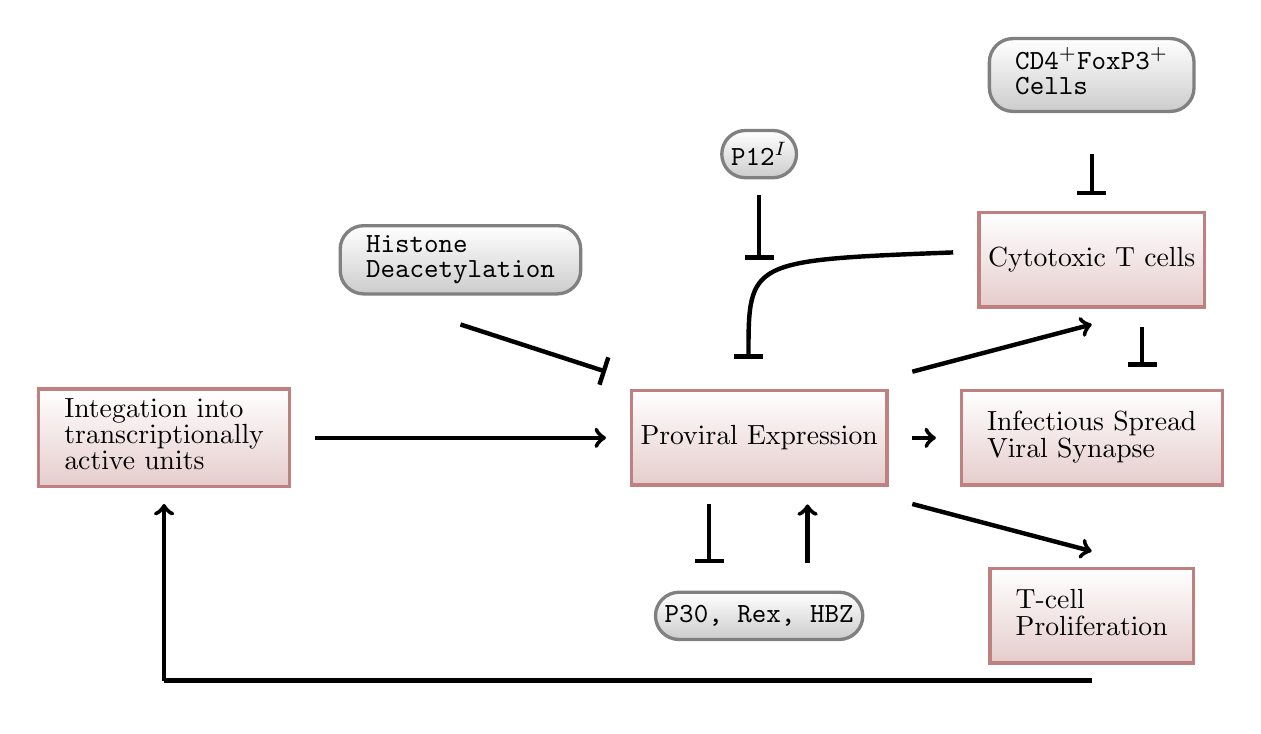
\begin{tikzpicture}[nonterminal/.style={
	rectangle,
	minimum size=12mm,
	very thick,
	draw=red!50!black!50, 
	top color=white, 
	bottom color=red!50!black!20
%	font=\itshape
	},terminal/.style={
	rectangle,minimum size=6mm,rounded corners=3mm,
	very thick,draw=black!50,
	top color=white,bottom color=black!20,
	font=\ttfamily
	},point/.style={
	circle,inner sep=0pt,minimum size=2pt,fill=red
	},point1/.style={
	coordinate,thick,draw=black!50
	}
]

\matrix[row sep=2mm,column sep=3mm] {
& & & & & & & \node (atom3) [terminal] {{\renewcommand{\arraystretch}{0.75}\begin{tabular}{l} CD4$^+$FoxP3$^+$ \\ Cells \end{tabular}}};
\\
 & & & & \node (atomP12) [terminal] {P12$^I$}; & & & \node (POSP) [point1] {.}; \\
 & & & & \node (POSY) [point1] {.}; & & & \node (POSQ) [point1] {.}; \\
% First row
 & & \node (atomHIS) [terminal] {{\renewcommand{\arraystretch}{0.75}\begin{tabular}{l} Histone \\ Deacetylation \end{tabular}}}; & & \node (POSZ) [point1] {.}; & & \node (POSO) [point1] {.}; & \node (atomCTL) [nonterminal] {Cytotoxic T cells}; \\
 & & \node (POSI) [point1] {.}; & & & & & \node (POSF) [point1] {.}; \\
 & & & & & & & \\
 & & & & & & & \\
 & & & \node (POSJ) [point1] {.}; & \node (POSN) [point1] {.}; & \node (POSE) [point1] {.}; & & \\
% Second row
\node (atom1) [nonterminal] {{\renewcommand{\arraystretch}{0.75}\begin{tabular}{l} Integation into \\ transcriptionally \\ active units \end{tabular}}}; & \node (POSA) [point1] {.}; & & \node (POSB) [point1] {.}; & \node (atom2) [nonterminal] {Proviral Expression}; & \node (POSC) [point1] {.}; & \node (POSD) [point1] {.}; & \node (atom3) [nonterminal] {{\renewcommand{\arraystretch}{0.75}\begin{tabular}{l} Infectious Spread \\ Viral Synapse \end{tabular}}};\\
\node (POSM) [point1] {.}; & & & & \node (POSR) [point1] {.}; & \node (POSG) [point1] {.}; & & \\
 & & & & & & & \\
 & & & & & & & \\
 & & & & \node (POSS) [point1] {.}; & & & \node (POSH) [point1] {.}; \\
% Third row
 & & & & \node (atomProt) [terminal] {P30, Rex, HBZ}; & & & \node (atomProl) [nonterminal] {{\renewcommand{\arraystretch}{0.75}\begin{tabular}{l} T-cell \\ Proliferation \end{tabular}}};\\
\node (POSK) [point1] {.}; & & & & & & & \node (POSL) [point1] {.}; \\
\\
};

%(x,y)
\draw[-|, ultra thick] (4.1,1.45) .. controls (1.5,1.35) .. (1.5,0.1);
\draw[ultra thick]	(POSA) edge[->] (POSB);
\draw[ultra thick]	(POSC) edge[->] (POSD);
\draw[ultra thick]	(POSE) edge[->] (POSF);
\draw[ultra thick]	(POSG) edge[->] (POSH);
\draw[ultra thick]	(POSI) edge[-|] (POSJ);
\draw[ultra thick]	(POSK) edge[-] (POSL);
\draw[ultra thick]	(POSK) edge[->] (POSM);
\draw[ultra thick]	(POSP) edge[-|] (POSQ);
\draw[ultra thick]	(POSY) edge[-|] (POSZ);
\draw[-|, ultra thick] (1,-1.75) -- (1,-2.5);
\draw[<-, ultra thick] (2.25,-1.75) -- (2.25,-2.5);
\draw[-|, ultra thick] (6.5,0.5) -- (6.5,0);

\end{tikzpicture}

\end{sideways}
\end{center}
\caption[The persistence of HTLV-I \emph{in vivo}]{The persistence of HTLV-I \emph{in vivo}. The stimulatory and inhibitory factors controlling HTLV-I proliferation (C.~Bangham, pers.~comm.).}
\label{chapter8/HTLVpers}
\end{table}

%%%%%%%%%%%%%%%%%%%%%%%%%%%%%%%%%%%%%%%%%%%%%%%%%%%%%%%%%%%%%%%%%%%%%%%%%%%%%%%%%%%%%%%%%%%%%%%%%%%%
%%%%%%%%%%%%%%%%%%%%%%%%%%%%%%%%%%%%%%%%%%%%%%%%%%%%%%%%%%%%%%%%%%%%%%%%%%%%%%%%%%%%%%%%%%%%%%%%%%%%	% General Discussion
%\input{./Chapters/Chapter10}	% Template Chapter

%% ----------------------------------------------------------------
% Now begin the Appendices, including them as separate files

\addtocontents{toc}{\vspace{2em}}	% Add a gap in the Contents, for aesthetics

\appendix	% Cue to tell LaTeX that the following 'chapters' are Appendices

% Appendix A

\chapter{Supplementary Data for Chapter 4}\label{AppendixA}
\lhead{Appendix A. \emph{Supplementary Data for Chapter 4}}

\section{Datasets}

The epitope datasets used in \cref{Chapter4} are detailed below. Each table gives the epitope, MHC class I allele and source protein of the epitope.

\clearpage

\begin{table}[htp]
\begin{center}
\begin{sideways}
{
\scriptsize
\begin{tabulary}{1.5\textwidth}{|l|l|l|l|l|l|l|l|l|l|l|l|}
\hline
Epitope & Allele & Protein & Start & Epitope & Allele & Protein & Start & Epitope & Allele & Protein & Start\bigstrut \\
\hline
AYSSWMYSY & A1 & EBN3\_EBV & 44 & SVASTITGV & A2 & ADFP\_HUMAN & 129 & NAYEYFTKI & B7 & BAK2\_HUMAN & 106 \bigstrut[t] \\
AIVDKVPSV & A2 & COPG\_HUMAN & 147 & SVFAGVVGV & A2 & CYG3\_HUMAN & 581 & NAYVNINRI & B7 & HAPP\_HUMAN & 363 \\
ALADGVQKV & A2 & APL1\_HUMAN & 160 & TIHDIILEC & A2 & VE6\_HPV16 & 29 & NPVPVGNIY & B7 & GAG\_HV2G1 & 257 \\
ALANGIEEV & A2 & APL3\_HUMAN & 172 & TILLGIFFL & A2 & MSHR\_HUMAN & 244 & NSSKVSQNY & B7 & GAG\_HV1J3 & 123 \\
ALASHLIEA & A2 & EHD2\_HUMAN & 507 & VLEETSVML & A2 & VIE1\_HCMVA & 316 & PPIPVGDIY & B7 & GAG\_HV1MA & 259 \\
ALFGALFLA & A2 & PLTP\_HUMAN & 2 & VMAPRTLVL & A2 & 1A23\_HUMAN & 3 & PPSGKGGNY & B7 & GAG\_HV2CA & 127 \\
ALLNIKVKL & A2 & K1CR\_HUMAN & 364 & WLNEVEFKL & A2 & DMD\_HUMAN & 1281 & SPKLPVSSL & B7 & DRI1\_HUMAN & 372 \\
ALLVLYSFA & A2 & LMP1\_EBV & 51 & YLDNGVVFV & A2 & DDB1\_HUMAN & 316 & SPYQNIKIL & B7 & SPSY\_HUMAN & 145 \\
ALPHAILRL & A2 & ACTB\_HUMAN & 170 & YLVTRHADV & A2 & POLG\_HCVH & 1131 & TSEHSHFSL & B7 & DCE2\_HUMAN & 277 \\
FLALIICNA & A2 & MSHR\_HUMAN & 283 & YVDPVITSI & A2 & MET\_HUMAN & 654 & TVLDVGDAY & B7 & POL\_HV1BR & 274 \\
FLDGNELTL & A2 & CLI1\_HUMAN & 167 & DADKYAVTV & B7 & OM1E\_CHLTR & 367 & VFPTKDVAL & B7 & PP65\_HCMVA & 187 \\
FLDGNEMTL & A2 & CLI4\_HUMAN & 178 & DAEMTTRMV & B7 & PSBA\_HUMAN & 90 & VPSEPGGVL & B7 & PTN6\_HUMAN & 422 \\
FLDPRPLTV & A2 & CP1B\_HUMAN & 190 & DAENAMRYI & B7 & CB20\_HUMAN & 93 & WASRELERF & B7 & GAG\_HV1BR & 35 \\
FLLDKKIGV & A2 & TCPB\_HUMAN & 218 & DALLIIPKV & B7 & TCPW\_HUMAN & 441 & YAFNMKATV & B7 & HS7C\_HUMAN & 545 \\
GLIEKNIEL & A2 & DNM1\_HUMAN & 425 & DALLKFSHI & B7 & BI1\_HUMAN & 11 & ELRRKMMYM & B8 & VIE1\_HCMVA & 199 \\
GLLGTLVQL & A2 & CTNB\_HUMAN & 400 & DALLQMITI & B7 & EF2\_HUMAN & 347 & ELRSRYWAI & B8 & VNUC\_IAPUE & 380 \\
GLYPGLIWL & A2 & IRF6\_HUMAN & 21 & DALRSILTI & B7 & SYM\_HUMAN & 703 & GEIYKRWII & B8 & GAG\_HV1BR & 258 \\
KASEKIFYV & A2 & SSX2\_HUMAN & 41 & DAYVLPKLY & B7 & RS26\_HUMAN & 60 & VMLRWGVLA & B8 & NCAP\_HRSVA & 256 \\
LLFDRPMHV & A2 & ROM\_HUMAN & 268 & DGYEQAARV & B7 & TCPE\_HUMAN & 135 & WVKEKVVAL & B8 & NK4\_HUMAN & 175 \\
LLMGTLGIV & A2 & VE7\_HPV16 & 82 & DPYEVSYRI & B7 & BTG1\_HUMAN & 107 & ARFGLIQSM & B27 & Y174\_HUMAN & 81 \\
LTAGFLIFL & A2 & LMP2\_EBV & 453 & DPYKVYRIV & B7 & IRF4\_HUMAN & 120 & GRFSGLLGR & B27 & IL16\_HUMAN & 180 \\
NLLPKLHIV & A2 & CLI1\_HUMAN & 179 & FAYVQIKTI & B7 & CP51\_HUMAN & 454 & GRNVVLDKS & B27 & CH60\_YEREN & 35 \\
NLTISDVSV & A2 & MUC1\_HUMAN & 1133 & HPDIVIYQY & B7 & POL\_HV1U4 & 329 & IRAAPPPLF & B27 & PRTP\_HUMAN & 2 \\
QLIDKVWQL & A2 & SC14\_HUMAN & 593 & IPQQHTQVL & B7 & CEA5\_HUMAN & 632 & IRAASAITA & B27 & CH60\_YEREN & 420 \\
RLVDDFLLV & A2 & TERT\_HUMAN & 865 & KPAFFAEKL & B7 & ANX1\_HUMAN & 273 & IRGAIILAK & B27 & RS2\_HUMAN & 151 \\
SLFPGKLEV & A2 & FLIH\_HUMAN & 1010 & KPSLPFTSL & B7 & CYRG\_HUMAN & 3 & IRLRPGGKK & B27 & GAG\_HV1BR & 18 \\
SLIGHLQTL & A2 & DUS5\_HUMAN & 337 & LPRSTVINI & B7 & IFM1\_HUMAN & 19 & IRNDEELNK & B27 & H2AC\_HUMAN & 87 \\
SLSEKTVLL & A2 & CD59\_HUMAN & 106 & MPMNVADLI & B7 & IF42\_HUMAN & 399 & IRRGVMLAV & B27 & CH60\_HUMAN & 140 \\
SLWGQPAEA & A2 & CA54\_HUMAN & 18 & MPWFKGWKV & B7 & EF11\_HUMAN & 208 & KRGIDKAVI & B27 & CH60\_YEREN & 117 \\
STAPPVHNV & A2 & MUC1\_HUMAN & 950 & NAACMALNI & B7 & OM1E\_CHLTR & 121 & KRIQEIIEQ & B27 & CH60\_HUMAN & 369 \bigstrut[b] \\
\hline
\end{tabulary}
}
\end{sideways}
\end{center}
\caption[The SYF$^1$ dataset]{The SYF$^1$ dataset.}\label{appendixa/table1}
\end{table}

\begin{table}[htp]
\begin{center}
\begin{sideways}
{
\scriptsize
\begin{tabulary}{1.5\textwidth}{|l|l|l|l|l|l|l|l|}
\hline
Epitope & Allele & Protein & Start & Epitope & Allele & Protein & Start \bigstrut \\
\hline
KRTLKIPAM & B27 & CH60\_HUMAN & 469 & ALNFPGSQK & A3 & PM17\_HUMAN & 87 \bigstrut[t] \\
MRMATPLLM & B27 & HG2A\_HUMAN & 107 & RLGVRATRK & A3 & POLG\_HCV1 & 43 \\
NRIVYLYTK & B27 & RL34\_HUMAN & 27 & GPISGHVLK & A3 & PP65\_HCMVA & 16 \\
QRNLYIAGF & B27 & CDM\_HUMAN & 100 & YTPTISRER & A3 & PSB2\_HUMAN & 147 \\
QRNVNIFKF & B27 & LDHA\_HUMAN & 110 & QAIKGMHIR & A3 & RL17\_HUMAN & 34 \\
QRVNVQPEL & B27 & PGTB\_HUMAN & 321 & SLADIMAKR & A3 & RL24\_HUMAN & 86 \\
TRYQGVNLY & B27 & PAB1\_HUMAN & 289 & DTIEIITDR & A3 & ROA2\_HUMAN & 139 \\
AENLWVTVY & B44 & ENV\_HV1S3 & 30 & ETIGEILKK & A3 & ROK\_HUMAN & 95 \\
AETPDIKLF & B44 & RS5\_HUMAN & 12 & FCVGFTKKR & A3 & RS3A\_HUMAN & 137 \\
NEGLGWAGW & B44 & POLG\_HCVJ6 & 88 & EVVVSGKLR & A3 & RS3\_HUMAN & 135 \\
IALYLQQNW & B58 & LMP1\_EBV & 156 & ETFSGVYKK & A3 & RS7\_HUMAN & 171 \\
ITTKAISRW & B58 & TCPG\_HUMAN & 159 & STIEYVIQR & A3 & S23B\_HUMAN & 115 \\
KTKEVIQEW & B58 & TALI\_HUMAN & 343 & TPAGGGFPR & A3 & TISB\_HUMAN & 43 \\
VSFIEFVGW & B58 & EBN4\_EBV & 279 & AIYKQSQHM & A24 & P53\_HUMAN & 161 \\
AFHHVAREL & B62 & NEF\_HV1BR & 190 & AYSQQTRGL & A24 & POLG\_HCVBK & 1031 \\
GFYPGSIEV & B62 & HB2I\_HUMAN & 150 & EYLQLVFGI & A24 & MAG2\_HUMAN & 156 \\
IKADHVSTY & B62 & HA2Q\_HUMAN & 32 & EYLVSFGVW & A24 & CORA\_HPBVJ & 117 \\
WQYFFPVIF & B62 & MAG3\_HUMAN & 143 & HYTNASDGL & A24 & LCK\_HUMAN & 207 \\
DTAAQITQR & A3 & 1B35\_HUMAN & 161 & KYTSFPWLL & A24 & DPOL\_HPBVJ & 756 \\
TIIDILTKR & A3 & ANX1\_HUMAN & 63 & QFQSIYAKF & A24 & RECO\_HUMAN & 47 \\
TIVNILTNR & A3 & ANX2\_HUMAN & 54 & QYDPVAALF & A24 & PP65\_HCMVA & 341 \\
TIIDIITHR & A3 & ANX6\_HUMAN & 384 & RWPSCQKKF & A24 & WT1\_HUMAN & 417 \\
ATIGTAMYK & A3 & BRL1\_EBV & 134 & TFDYLRSVL & A24 & LCK\_HUMAN & 485 \\
GSPATWTTR & A3 & CA34\_HUMAN & 1436 & TYGEIFEKF & A24 & N4BM\_HUMAN & 107 \\
YVNVNMGLK & A3 & CORA\_HPBV4 & 88 & VYAETKHFL & A24 & TERT\_HUMAN & 324 \\
RFKMFPEVK & A3 & DCE2\_HUMAN & 255 & VYALPLKML & A24 & PP65\_HCMVA & 113 \\
TLYCVHQRI & A3 & GAG\_HV1BR & 83 & VYGFVRACL & A24 & TERT\_HUMAN & 461 \\
IVGLNKIVR & A3 & GAG\_HV1EL & 266 & YYMIGEQKF & A24 & NNMT\_HUMAN & 203 \\
DVFVVGTER & A3 & GTFI\_HUMAN & 53 &  &  &  & \\
SIMKWNRER & A3 & NB6M\_HUMAN & 48 &  &  &  & \bigstrut[b] \\
\hline
\end{tabulary}
}
\end{sideways}
\end{center}
\contcaption{Continued}
\end{table}





\begin{table}[htp]
\begin{center}
\begin{sideways}
{
\scriptsize
\begin{tabulary}{1.5\textwidth}{|l|l|l|l|l|l|l|l|l|l|l|l|}
\hline
Epitope & Allele & Protein & HXB2 & Epitope & Allele & Protein & HXB2 & Epitope & Allele & Protein & HXB2 \bigstrut \\
\hline
RRGWEALKY & A1 & gp160 & 787 & TLNAWVKVV & A2 & p24-p2p7p1 & 19 & RLRPGGKKK & A3 & p17 & 20 \bigstrut[t] \\
WIYHTQGYF & A1 & Nef & 113 & AMQMLKETI & A2 & p24-p2p7p1 & 65 & TVRLIKLLY & A3 & Rev & 15 \\
YFPDWQNYT & A1 & Nef & 120 & AEWDRVHPV & A2 & p24-p2p7p1 & 78 & KLLYQSNPP & A3 & Rev & 20 \\
GSEELRSLY & A1 & p17 & 71 & TLQEQIGWM & A2 & p24-p2p7p1 & 110 & RILGTYLGR & A3 & Rev & 58 \\
QRPLVTIKI & A1 & Protease & 7 & MTNNPPIPV & A2 & p24-p2p7p1 & 118 & ALVEICTEM & A3 & RT & 33 \\
ISERILGTY & A1 & Rev & 55 & RMYSPTSIL & A2 & p24-p2p7p1 & 143 & NTPVFAIKK & A3 & RT & 57 \\
LWVTVYYGV & A2 & gp160 & 34 & YVDRFYKTL & A2 & p24-p2p7p1 & 164 & GIPHPAGLK & A3 & RT & 93 \\
VTVYYGVPV & A2 & gp160 & 36 & VLAEAMSQV & A2 & p24-p2p7p1 & 230 & AIFQSSMTK & A3 & RT & 158 \\
NVWATHACV & A2 & gp160 & 67 & LVGPTPVNI & A2 & Protease & 76 & QIYPGIKVR & A3 & RT & 269 \\
QMHEDIISL & A2 & gp160 & 103 & ALVEICTEM & A2 & RT & 33 & QIIEQLIKK & A3 & RT & 520 \\
KLTPLCVSL & A2 & gp160 & 121 & YTAFTIPSI & A2 & RT & 127 & KVYLAWVPA & A3 & RT & 530 \\
KLTSCNTSV & A2 & gp160 & 192 & VIYQYMDDL & A2 & RT & 179 & TACTNCYCK & A3 & Tat & 20 \\
QRGPGRAFV & A2 & gp160 & 310 & YQYMDDLYV & A2 & RT & 181 & HMYVSGKAR & A3 & Vif & 28 \\
TLKQIASKL & A2 & gp160 & 341 & KIEELRQHL & A2 & RT & 201 & KLTEDRWNK & A3 & Vif & 168 \\
TMGAASMTL & A2 & gp160 & 529 & ILKEPVHGV & A2 & RT & 309 & IQRGPGRAF & A24 & gp160 & 309 \\
AVLSIVNRV & A2 & gp160 & 700 & PLVKLWYQL & A2 & RT & 421 & FYCNSTQLF & A24 & gp160 & 383 \\
RLVNGSLAL & A2 & gp160 & 747 & KLGKAGYVT & A2 & RT & 451 & RYLKDQQLL & A24 & gp160 & 585 \\
RLRDLLLIV & A2 & gp160 & 770 & ALQDSGLEV & A2 & RT & 485 & WYIKLFIMI & A24 & gp160 & 680 \\
LLNATAIAV & A2 & gp160 & 814 & AIIRILQQL & A2 & Vpr & 59 & SYHRLRDLL & A24 & gp160 & 767 \\
RVIEVVQGA & A2 & gp160 & 828 & RILQQLLFI & A2 & Vpr & 62 & HSQRRQDIL & A24 & Nef & 102 \\
RIRQGLERI & A2 & gp160 & 846 & VVAIIIAIV & A2 & Vpu & 13 & RQDILDLWI & A24 & Nef & 106 \\
QVRDQAEHL & A2 & Integrase & 164 & SLWDQSLKP & A3 & gp160 & 110 & GYFPDWQNY & A24 & Nef & 119 \\
LLWKGEGAV & A2 & Integrase & 241 & VSFEPIPIH & A3 & gp160 & 208 & DSRLAFHHV & A24 & Nef & 186 \\
ATNAACAWL & A2 & Nef & 50 & HSFNCGGEF & A3 & gp160 & 374 & AFHHVAREL & A24 & Nef & 190 \\
AAVDLSHFL & A2 & Nef & 83 & AVDLSHFLK & A3 & Nef & 84 & KYKLKHIVW & A24 & p17 & 28 \\
YPLTFGWCY & A2 & Nef & 135 & DLSHFLKEK & A3 & Nef & 86 & EIYKRWIIL & A24 & p24-p2p7p1 & 128 \\
LTFGWCYKL & A2 & Nef & 137 & ILDLWIYHT & A3 & Nef & 109 & DYVDRFYKT & A24 & p24-p2p7p1 & 163 \\
LEWRFDSRL & A2 & Nef & 181 & PLTFGWCYK & A3 & Nef & 136 & VYYDPSKDL & A24 & RT & 317 \\
AFHHVAREL & A2 & Nef & 190 & AFHHVAREL & A3 & Nef & 190 & IYQEPFKNL & A24 & RT & 341 \\
SLYNTVATL & A2 & p17 & 77 & KIRLRPGGK & A3 & p17 & 18 & EVIPMFSAL & A26 & p24-p2p7p1 & 35 \bigstrut[b] \\	
\hline
\end{tabulary}
}
\end{sideways}
\end{center}
\caption[The Lanl$^{179}$ dataset]{The Lanl$^{179}$ dataset.}\label{appendixa/table2}
\end{table}

\begin{table}[htp]
\begin{center}
\begin{sideways}
{
\scriptsize
\begin{tabulary}{1.5\textwidth}{|l|l|l|l|l|l|l|l|l|l|l|l|}
\hline
Epitope & Allele & Protein & HXB2 & Epitope & Allele & Protein & HXB2 & Epitope & Allele & Protein & HXB2 \bigstrut \\
\hline
YVDRFYKTL & A26 & p24-p2p7p1 & 164 & GRAFVTIGK & B27 & gp160 & 314 & IVLPEKDSW & B58 & RT & 244 \bigstrut[t] \\
ETKLGKAGY & A26 & RT & 449 & GRRGWEALK & B27 & gp160 & 786 & ITTESIVIW & B58 & RT & 375 \\
IPRRIRQGL & B7 & gp160 & 843 & KIRLRPGGK & B27 & p17 & 18 & VSGKARGWF & B58 & Vif & 31 \\
LPPVVAKEI & B7 & Integrase & 28 & IRLRPGGKK & B27 & p17 & 19 & AVRHFPRIW & B58 & Vpr & 30 \\
FPVTPQVPL & B7 & Nef & 68 & KRWIILGLN & B27 & p24-p2p7p1 & 131 & SFNCGGEFF & B62 & gp160 & 375 \\
TPQVPLRPM & B7 & Nef & 71 & RWIILGLNK & B27 & p24-p2p7p1 & 132 & RAIEAQQHL & B62 & gp160 & 557 \\
RPMTYKAAV & B7 & Nef & 77 & VRHFPRIWL & B27 & Vpr & 31 & THLEGKVIL & B62 & Integrase & 66 \\
TPGPGVRYP & B7 & Nef & 128 & TPQDLNTML & B39 & p24-p2p7p1 & 48 & IKQEFGIPY & B62 & Integrase & 135 \\
YPLTFGWCY & B7 & Nef & 135 & HPVHAGPIA & B39 & p24-p2p7p1 & 84 & RKAKIIRDY & B62 & Integrase & 263 \\
KIRLRPGGK & B7 & p17 & 18 & LEKHGAITS & B44 & Nef & 37 & RMRRAEPAA & B62 & Nef & 19 \\
SPRTLNAWV & B7 & p24-p2p7p1 & 16 & AAVDLSHFL & B44 & Nef & 83 & MTYKAAVDL & B62 & Nef & 79 \\
ATPQDLNTM & B7 & p24-p2p7p1 & 47 & KEKGGLEGL & B44 & Nef & 92 & AAVDLSHFL & B62 & Nef & 83 \\
TPQDLNTML & B7 & p24-p2p7p1 & 48 & GELDRWEKI & B44 & p17 & 11 & YFPDWQNYT & B62 & Nef & 120 \\
HPVHAGPIA & B7 & p24-p2p7p1 & 84 & SEGATPQDL & B44 & p24-p2p7p1 & 44 & LTFGWCYKL & B62 & Nef & 137 \\
ANPDCKTIL & B7 & p24-p2p7p1 & 194 & KETINEEAA & B44 & p24-p2p7p1 & 70 & WRFDSRLAF & B62 & Nef & 183 \\
GPGHKARVL & B7 & p24-p2p7p1 & 223 & EEAAEWDRV & B44 & p24-p2p7p1 & 75 & RLRPGGKKK & B62 & p17 & 20 \\
YPLTSLRSL & B7 & p24-p2p7p1 & 352 & AEWDRVHPV & B44 & p24-p2p7p1 & 78 & RFAVNPGLL & B62 & p17 & 43 \\
SPAIFQSSM & B7 & RT & 156 & CTERQANFL & B44 & p24-p2p7p1 & 294 & VKVVEEKAF & B62 & p24-p2p7p1 & 24 \\
IPLTEEAEL & B7 & RT & 293 & KELYPLTSL & B44 & p24-p2p7p1 & 349 & FSPEVIPMF & B62 & p24-p2p7p1 & 32 \\
YLAWVPAHK & B7 & RT & 532 & IEELRQHLL & B44 & RT & 202 & GHQAAMQML & B62 & p24-p2p7p1 & 61 \\
FPRIWLHGL & B7 & Vpr & 34 & REPHNEWTL & B44 & Vpr & 12 & GLNKIVRMY & B62 & p24-p2p7p1 & 137 \\
RVKEKYQHL & B8 & gp160 & 2 & RAIEAQQHL & B58 & gp160 & 557 & YVDRFYKTL & B62 & p24-p2p7p1 & 164 \\
FNCGGEFFY & B8 & gp160 & 376 & KTAVQMAVF & B58 & Integrase & 173 & GHKAIGTVL & B62 & Protease & 68 \\
GGKKKYKLK & B8 & p17 & 24 & KAAVDLSHF & B58 & Nef & 82 & IHSISERIL & B62 & Rev & 52 \\
ELRSLYNTV & B8 & p17 & 74 & HTQGYFPDW & B58 & Nef & 116 & IPLTEEAEL & B62 & RT & 293 \\
EIKDTKEAL & B8 & p17 & 93 & YTPGPGVRY & B58 & Nef & 127 & DVKQLTEAV & B62 & RT & 364 \\
GEIYKRWII & B8 & p24-p2p7p1 & 127 & ISPRTLNAW & B58 & p24-p2p7p1 & 15 & ITKALGISY & B62 & Tat & 39 \\
NANPDCKTI & B8 & p24-p2p7p1 & 193 & FSPEVIPMF & B58 & p24-p2p7p1 & 32 & WHLGQGVSI & B62 & Vif & 79 \\
DCKTILKAL & B8 & p24-p2p7p1 & 197 & STLQEQIGW & B58 & p24-p2p7p1 & 109 & AVRHFPRIW & B62 & Vpr & 30 \\
GPKVKQWPL & B8 & RT & 18 & QASQEVKNW & B58 & p24-p2p7p1 & 176 & & & & \bigstrut[b] \\		
\hline
\end{tabulary}
}
\end{sideways}
\end{center}
\contcaption{Continued}
\end{table}

\begin{table}[htp]
\begin{center}
\begin{sideways}
{
\tiny
\begin{tabulary}{1.5\textwidth}{|l|l|l|l|l|l|l|l|l|l|l|l|}
\hline
Epitope & Allele & Protein & HXB2 & Epitope & Allele & Protein & HXB2 & Epitope & Allele & Protein & HXB2 \bigstrut \\
\hline
RRGWEALKY & A0101 & gp160 & 787 & KLTSCNTSV & A0202 & gp160 & 192 & LLWKGEGAV & A0203 & Integrase & 241 \bigstrut[t] \\
WIYHTQGYF & A0101 & Nef & 113 & QRGPGRAFV & A0202 & gp160 & 310 & ATNAACAWL & A0203 & Nef & 50 \\
YFPDWQNYT & A0101 & Nef & 120 & TLKQIASKL & A0202 & gp160 & 341 & AAVDLSHFL & A0203 & Nef & 83 \\
GSEELRSLY & A0101 & p17 & 71 & TMGAASMTL & A0202 & gp160 & 529 & YPLTFGWCY & A0203 & Nef & 135 \\
QRPLVTIKI & A0101 & Protease & 7 & AVLSIVNRV & A0202 & gp160 & 700 & LTFGWCYKL & A0203 & Nef & 137 \\
ISERILGTY & A0101 & Rev & 55 & RLVNGSLAL & A0202 & gp160 & 747 & LEWRFDSRL & A0203 & Nef & 181 \\
LWVTVYYGV & A0201 & gp160 & 34 & RLRDLLLIV & A0202 & gp160 & 770 & AFHHVAREL & A0203 & Nef & 190 \\
VTVYYGVPV & A0201 & gp160 & 36 & LLNATAIAV & A0202 & gp160 & 814 & SLYNTVATL & A0203 & p17 & 77 \\
NVWATHACV & A0201 & gp160 & 67 & RVIEVVQGA & A0202 & gp160 & 828 & TLNAWVKVV & A0203 & p24-p2p7p1 & 19 \\
QMHEDIISL & A0201 & gp160 & 103 & RIRQGLERI & A0202 & gp160 & 846 & AMQMLKETI & A0203 & p24-p2p7p1 & 65 \\
KLTPLCVSL & A0201 & gp160 & 121 & QVRDQAEHL & A0202 & Integrase & 164 & AEWDRVHPV & A0203 & p24-p2p7p1 & 78 \\
KLTSCNTSV & A0201 & gp160 & 192 & LLWKGEGAV & A0202 & Integrase & 241 & TLQEQIGWM & A0203 & p24-p2p7p1 & 110 \\
QRGPGRAFV & A0201 & gp160 & 310 & ATNAACAWL & A0202 & Nef & 50 & MTNNPPIPV & A0203 & p24-p2p7p1 & 118 \\
TLKQIASKL & A0201 & gp160 & 341 & AAVDLSHFL & A0202 & Nef & 83 & RMYSPTSIL & A0203 & p24-p2p7p1 & 143 \\
TMGAASMTL & A0201 & gp160 & 529 & YPLTFGWCY & A0202 & Nef & 135 & YVDRFYKTL & A0203 & p24-p2p7p1 & 164 \\
AVLSIVNRV & A0201 & gp160 & 700 & LTFGWCYKL & A0202 & Nef & 137 & VLAEAMSQV & A0203 & p24-p2p7p1 & 230 \\
RLVNGSLAL & A0201 & gp160 & 747 & LEWRFDSRL & A0202 & Nef & 181 & LVGPTPVNI & A0203 & Protease & 76 \\
RLRDLLLIV & A0201 & gp160 & 770 & AFHHVAREL & A0202 & Nef & 190 & ALVEICTEM & A0203 & RT & 33 \\
LLNATAIAV & A0201 & gp160 & 814 & SLYNTVATL & A0202 & p17 & 77 & YTAFTIPSI & A0203 & RT & 127 \\
RVIEVVQGA & A0201 & gp160 & 828 & TLNAWVKVV & A0202 & p24-p2p7p1 & 19 & VIYQYMDDL & A0203 & RT & 179 \\
RIRQGLERI & A0201 & gp160 & 846 & AMQMLKETI & A0202 & p24-p2p7p1 & 65 & YQYMDDLYV & A0203 & RT & 181 \\
QVRDQAEHL & A0201 & Integrase & 164 & AEWDRVHPV & A0202 & p24-p2p7p1 & 78 & KIEELRQHL & A0203 & RT & 201 \\
LLWKGEGAV & A0201 & Integrase & 241 & TLQEQIGWM & A0202 & p24-p2p7p1 & 110 & ILKEPVHGV & A0203 & RT & 309 \\
ATNAACAWL & A0201 & Nef & 50 & MTNNPPIPV & A0202 & p24-p2p7p1 & 118 & PLVKLWYQL & A0203 & RT & 421 \\
AAVDLSHFL & A0201 & Nef & 83 & RMYSPTSIL & A0202 & p24-p2p7p1 & 143 & KLGKAGYVT & A0203 & RT & 451 \\
YPLTFGWCY & A0201 & Nef & 135 & YVDRFYKTL & A0202 & p24-p2p7p1 & 164 & ALQDSGLEV & A0203 & RT & 485 \\
LTFGWCYKL & A0201 & Nef & 137 & VLAEAMSQV & A0202 & p24-p2p7p1 & 230 & AIIRILQQL & A0203 & Vpr & 59 \\
LEWRFDSRL & A0201 & Nef & 181 & LVGPTPVNI & A0202 & Protease & 76 & RILQQLLFI & A0203 & Vpr & 62 \\
AFHHVAREL & A0201 & Nef & 190 & ALVEICTEM & A0202 & RT & 33 & VVAIIIAIV & A0203 & Vpu & 13 \\
SLYNTVATL & A0201 & p17 & 77 & YTAFTIPSI & A0202 & RT & 127 & LWVTVYYGV & A0206 & gp160 & 34 \\
TLNAWVKVV & A0201 & p24-p2p7p1 & 19 & VIYQYMDDL & A0202 & RT & 179 & VTVYYGVPV & A0206 & gp160 & 36 \\
AMQMLKETI & A0201 & p24-p2p7p1 & 65 & YQYMDDLYV & A0202 & RT & 181 & NVWATHACV & A0206 & gp160 & 67 \\
AEWDRVHPV & A0201 & p24-p2p7p1 & 78 & KIEELRQHL & A0202 & RT & 201 & QMHEDIISL & A0206 & gp160 & 103 \\
TLQEQIGWM & A0201 & p24-p2p7p1 & 110 & ILKEPVHGV & A0202 & RT & 309 & KLTPLCVSL & A0206 & gp160 & 121 \\
MTNNPPIPV & A0201 & p24-p2p7p1 & 118 & PLVKLWYQL & A0202 & RT & 421 & KLTSCNTSV & A0206 & gp160 & 192 \\
RMYSPTSIL & A0201 & p24-p2p7p1 & 143 & KLGKAGYVT & A0202 & RT & 451 & QRGPGRAFV & A0206 & gp160 & 310 \\
YVDRFYKTL & A0201 & p24-p2p7p1 & 164 & ALQDSGLEV & A0202 & RT & 485 & TLKQIASKL & A0206 & gp160 & 341 \\
VLAEAMSQV & A0201 & p24-p2p7p1 & 230 & AIIRILQQL & A0202 & Vpr & 59 & TMGAASMTL & A0206 & gp160 & 529 \\
LVGPTPVNI & A0201 & Protease & 76 & RILQQLLFI & A0202 & Vpr & 62 & AVLSIVNRV & A0206 & gp160 & 700 \\
ALVEICTEM & A0201 & RT & 33 & VVAIIIAIV & A0202 & Vpu & 13 & RLVNGSLAL & A0206 & gp160 & 747 \\
YTAFTIPSI & A0201 & RT & 127 & LWVTVYYGV & A0203 & gp160 & 34 & RLRDLLLIV & A0206 & gp160 & 770 \\
VIYQYMDDL & A0201 & RT & 179 & VTVYYGVPV & A0203 & gp160 & 36 & LLNATAIAV & A0206 & gp160 & 814 \\
YQYMDDLYV & A0201 & RT & 181 & NVWATHACV & A0203 & gp160 & 67 & RVIEVVQGA & A0206 & gp160 & 828 \\
KIEELRQHL & A0201 & RT & 201 & QMHEDIISL & A0203 & gp160 & 103 & RIRQGLERI & A0206 & gp160 & 846 \\
ILKEPVHGV & A0201 & RT & 309 & KLTPLCVSL & A0203 & gp160 & 121 & QVRDQAEHL & A0206 & Integrase & 164 \\
PLVKLWYQL & A0201 & RT & 421 & KLTSCNTSV & A0203 & gp160 & 192 & LLWKGEGAV & A0206 & Integrase & 241 \\
KLGKAGYVT & A0201 & RT & 451 & QRGPGRAFV & A0203 & gp160 & 310 & ATNAACAWL & A0206 & Nef & 50 \\
ALQDSGLEV & A0201 & RT & 485 & TLKQIASKL & A0203 & gp160 & 341 & AAVDLSHFL & A0206 & Nef & 83 \\
AIIRILQQL & A0201 & Vpr & 59 & TMGAASMTL & A0203 & gp160 & 529 & YPLTFGWCY & A0206 & Nef & 135 \\
RILQQLLFI & A0201 & Vpr & 62 & AVLSIVNRV & A0203 & gp160 & 700 & LTFGWCYKL & A0206 & Nef & 137 \\
VVAIIIAIV & A0201 & Vpu & 13 & RLVNGSLAL & A0203 & gp160 & 747 & LEWRFDSRL & A0206 & Nef & 181 \\
LWVTVYYGV & A0202 & gp160 & 34 & RLRDLLLIV & A0203 & gp160 & 770 & AFHHVAREL & A0206 & Nef & 190 \\
VTVYYGVPV & A0202 & gp160 & 36 & LLNATAIAV & A0203 & gp160 & 814 & SLYNTVATL & A0206 & p17 & 77 \\
NVWATHACV & A0202 & gp160 & 67 & RVIEVVQGA & A0203 & gp160 & 828 & TLNAWVKVV & A0206 & p24-p2p7p1 & 19 \\
QMHEDIISL & A0202 & gp160 & 103 & RIRQGLERI & A0203 & gp160 & 846 & AMQMLKETI & A0206 & p24-p2p7p1 & 65 \\
KLTPLCVSL & A0202 & gp160 & 121 & QVRDQAEHL & A0203 & Integrase & 164 & AEWDRVHPV & A0206 & p24-p2p7p1 & 78 \bigstrut[b] \\
\hline
\end{tabulary}
}
\end{sideways}
\end{center}
\caption[The Lanl$^{661}$ dataset]{The Lanl$^{661}$ dataset.}\label{appendixa/table3}
\end{table}

\begin{table}[htp]
\begin{center}
\begin{sideways}
{
\tiny
\begin{tabulary}{1.5\textwidth}{|l|l|l|l|l|l|l|l|l|l|l|l|}
\hline
Epitope & Allele & Protein & HXB2 & Epitope & Allele & Protein & HXB2 & Epitope & Allele & Protein & HXB2 \bigstrut \\
\hline
TLQEQIGWM & A0206 & p24-p2p7p1 & 110 & ILKEPVHGV & A0211 & RT & 309 & KLTPLCVSL & A0216 & gp160 & 121 \bigstrut[t] \\
MTNNPPIPV & A0206 & p24-p2p7p1 & 118 & PLVKLWYQL & A0211 & RT & 421 & KLTSCNTSV & A0216 & gp160 & 192 \\
RMYSPTSIL & A0206 & p24-p2p7p1 & 143 & KLGKAGYVT & A0211 & RT & 451 & QRGPGRAFV & A0216 & gp160 & 310 \\
YVDRFYKTL & A0206 & p24-p2p7p1 & 164 & ALQDSGLEV & A0211 & RT & 485 & TLKQIASKL & A0216 & gp160 & 341 \\
VLAEAMSQV & A0206 & p24-p2p7p1 & 230 & AIIRILQQL & A0211 & Vpr & 59 & TMGAASMTL & A0216 & gp160 & 529 \\
LVGPTPVNI & A0206 & Protease & 76 & RILQQLLFI & A0211 & Vpr & 62 & AVLSIVNRV & A0216 & gp160 & 700 \\
ALVEICTEM & A0206 & RT & 33 & VVAIIIAIV & A0211 & Vpu & 13 & RLVNGSLAL & A0216 & gp160 & 747 \\
YTAFTIPSI & A0206 & RT & 127 & LWVTVYYGV & A0212 & gp160 & 34 & RLRDLLLIV & A0216 & gp160 & 770 \\
VIYQYMDDL & A0206 & RT & 179 & VTVYYGVPV & A0212 & gp160 & 36 & LLNATAIAV & A0216 & gp160 & 814 \\
YQYMDDLYV & A0206 & RT & 181 & NVWATHACV & A0212 & gp160 & 67 & RVIEVVQGA & A0216 & gp160 & 828 \\
KIEELRQHL & A0206 & RT & 201 & QMHEDIISL & A0212 & gp160 & 103 & RIRQGLERI & A0216 & gp160 & 846 \\
ILKEPVHGV & A0206 & RT & 309 & KLTPLCVSL & A0212 & gp160 & 121 & QVRDQAEHL & A0216 & Integrase & 164 \\
PLVKLWYQL & A0206 & RT & 421 & KLTSCNTSV & A0212 & gp160 & 192 & LLWKGEGAV & A0216 & Integrase & 241 \\
KLGKAGYVT & A0206 & RT & 451 & QRGPGRAFV & A0212 & gp160 & 310 & ATNAACAWL & A0216 & Nef & 50 \\
ALQDSGLEV & A0206 & RT & 485 & TLKQIASKL & A0212 & gp160 & 341 & AAVDLSHFL & A0216 & Nef & 83 \\
AIIRILQQL & A0206 & Vpr & 59 & TMGAASMTL & A0212 & gp160 & 529 & YPLTFGWCY & A0216 & Nef & 135 \\
RILQQLLFI & A0206 & Vpr & 62 & AVLSIVNRV & A0212 & gp160 & 700 & LTFGWCYKL & A0216 & Nef & 137 \\
VVAIIIAIV & A0206 & Vpu & 13 & RLVNGSLAL & A0212 & gp160 & 747 & LEWRFDSRL & A0216 & Nef & 181 \\
LWVTVYYGV & A0211 & gp160 & 34 & RLRDLLLIV & A0212 & gp160 & 770 & AFHHVAREL & A0216 & Nef & 190 \\
VTVYYGVPV & A0211 & gp160 & 36 & LLNATAIAV & A0212 & gp160 & 814 & SLYNTVATL & A0216 & p17 & 77 \\
NVWATHACV & A0211 & gp160 & 67 & RVIEVVQGA & A0212 & gp160 & 828 & TLNAWVKVV & A0216 & p24-p2p7p1 & 19 \\
QMHEDIISL & A0211 & gp160 & 103 & RIRQGLERI & A0212 & gp160 & 846 & AMQMLKETI & A0216 & p24-p2p7p1 & 65 \\
KLTPLCVSL & A0211 & gp160 & 121 & QVRDQAEHL & A0212 & Integrase & 164 & AEWDRVHPV & A0216 & p24-p2p7p1 & 78 \\
KLTSCNTSV & A0211 & gp160 & 192 & LLWKGEGAV & A0212 & Integrase & 241 & TLQEQIGWM & A0216 & p24-p2p7p1 & 110 \\
QRGPGRAFV & A0211 & gp160 & 310 & ATNAACAWL & A0212 & Nef & 50 & MTNNPPIPV & A0216 & p24-p2p7p1 & 118 \\
TLKQIASKL & A0211 & gp160 & 341 & AAVDLSHFL & A0212 & Nef & 83 & RMYSPTSIL & A0216 & p24-p2p7p1 & 143 \\
TMGAASMTL & A0211 & gp160 & 529 & YPLTFGWCY & A0212 & Nef & 135 & YVDRFYKTL & A0216 & p24-p2p7p1 & 164 \\
AVLSIVNRV & A0211 & gp160 & 700 & LTFGWCYKL & A0212 & Nef & 137 & VLAEAMSQV & A0216 & p24-p2p7p1 & 230 \\
RLVNGSLAL & A0211 & gp160 & 747 & LEWRFDSRL & A0212 & Nef & 181 & LVGPTPVNI & A0216 & Protease & 76 \\
RLRDLLLIV & A0211 & gp160 & 770 & AFHHVAREL & A0212 & Nef & 190 & ALVEICTEM & A0216 & RT & 33 \\
LLNATAIAV & A0211 & gp160 & 814 & SLYNTVATL & A0212 & p17 & 77 & YTAFTIPSI & A0216 & RT & 127 \\
RVIEVVQGA & A0211 & gp160 & 828 & TLNAWVKVV & A0212 & p24-p2p7p1 & 19 & VIYQYMDDL & A0216 & RT & 179 \\
RIRQGLERI & A0211 & gp160 & 846 & AMQMLKETI & A0212 & p24-p2p7p1 & 65 & YQYMDDLYV & A0216 & RT & 181 \\
QVRDQAEHL & A0211 & Integrase & 164 & AEWDRVHPV & A0212 & p24-p2p7p1 & 78 & KIEELRQHL & A0216 & RT & 201 \\
LLWKGEGAV & A0211 & Integrase & 241 & TLQEQIGWM & A0212 & p24-p2p7p1 & 110 & ILKEPVHGV & A0216 & RT & 309 \\
ATNAACAWL & A0211 & Nef & 50 & MTNNPPIPV & A0212 & p24-p2p7p1 & 118 & PLVKLWYQL & A0216 & RT & 421 \\
AAVDLSHFL & A0211 & Nef & 83 & RMYSPTSIL & A0212 & p24-p2p7p1 & 143 & KLGKAGYVT & A0216 & RT & 451 \\
YPLTFGWCY & A0211 & Nef & 135 & YVDRFYKTL & A0212 & p24-p2p7p1 & 164 & ALQDSGLEV & A0216 & RT & 485 \\
LTFGWCYKL & A0211 & Nef & 137 & VLAEAMSQV & A0212 & p24-p2p7p1 & 230 & AIIRILQQL & A0216 & Vpr & 59 \\
LEWRFDSRL & A0211 & Nef & 181 & LVGPTPVNI & A0212 & Protease & 76 & RILQQLLFI & A0216 & Vpr & 62 \\
AFHHVAREL & A0211 & Nef & 190 & ALVEICTEM & A0212 & RT & 33 & VVAIIIAIV & A0216 & Vpu & 13 \\
SLYNTVATL & A0211 & p17 & 77 & YTAFTIPSI & A0212 & RT & 127 & LWVTVYYGV & A0219 & gp160 & 34 \\
TLNAWVKVV & A0211 & p24-p2p7p1 & 19 & VIYQYMDDL & A0212 & RT & 179 & VTVYYGVPV & A0219 & gp160 & 36 \\
AMQMLKETI & A0211 & p24-p2p7p1 & 65 & YQYMDDLYV & A0212 & RT & 181 & NVWATHACV & A0219 & gp160 & 67 \\
AEWDRVHPV & A0211 & p24-p2p7p1 & 78 & KIEELRQHL & A0212 & RT & 201 & QMHEDIISL & A0219 & gp160 & 103 \\
TLQEQIGWM & A0211 & p24-p2p7p1 & 110 & ILKEPVHGV & A0212 & RT & 309 & KLTPLCVSL & A0219 & gp160 & 121 \\
MTNNPPIPV & A0211 & p24-p2p7p1 & 118 & PLVKLWYQL & A0212 & RT & 421 & KLTSCNTSV & A0219 & gp160 & 192 \\
RMYSPTSIL & A0211 & p24-p2p7p1 & 143 & KLGKAGYVT & A0212 & RT & 451 & QRGPGRAFV & A0219 & gp160 & 310 \\
YVDRFYKTL & A0211 & p24-p2p7p1 & 164 & ALQDSGLEV & A0212 & RT & 485 & TLKQIASKL & A0219 & gp160 & 341 \\
VLAEAMSQV & A0211 & p24-p2p7p1 & 230 & AIIRILQQL & A0212 & Vpr & 59 & TMGAASMTL & A0219 & gp160 & 529 \\
LVGPTPVNI & A0211 & Protease & 76 & RILQQLLFI & A0212 & Vpr & 62 & AVLSIVNRV & A0219 & gp160 & 700 \\
ALVEICTEM & A0211 & RT & 33 & VVAIIIAIV & A0212 & Vpu & 13 & RLVNGSLAL & A0219 & gp160 & 747 \\
YTAFTIPSI & A0211 & RT & 127 & LWVTVYYGV & A0216 & gp160 & 34 & RLRDLLLIV & A0219 & gp160 & 770 \\
VIYQYMDDL & A0211 & RT & 179 & VTVYYGVPV & A0216 & gp160 & 36 & LLNATAIAV & A0219 & gp160 & 814 \\
YQYMDDLYV & A0211 & RT & 181 & NVWATHACV & A0216 & gp160 & 67 & RVIEVVQGA & A0219 & gp160 & 828 \\
KIEELRQHL & A0211 & RT & 201 & QMHEDIISL & A0216 & gp160 & 103 & RIRQGLERI & A0219 & gp160 & 846 \bigstrut[b] \\
\hline
\end{tabulary}
}
\end{sideways}
\end{center}
\contcaption{Continued}
\end{table}

\begin{table}[htp]
\begin{center}
\begin{sideways}
{
\tiny
\begin{tabulary}{1.5\textwidth}{|l|l|l|l|l|l|l|l|l|l|l|l|}
\hline
Epitope & Allele & Protein & HXB2 & Epitope & Allele & Protein & HXB2 & Epitope & Allele & Protein & HXB2 \bigstrut \\
\hline
QVRDQAEHL & A0219 & Integrase & 164 & DLSHFLKEK & A1101 & Nef & 86 & RLRPGGKKK & A3001 & p17 & 20 \bigstrut[t] \\
LLWKGEGAV & A0219 & Integrase & 241 & TLYCVHQRI & A1101 & p17 & 84 & KQNPDIVIY & A3001 & RT & 173 \\
ATNAACAWL & A0219 & Nef & 50 & AIFQSSMTK & A1101 & RT & 158 & KLNWASQIY & A3001 & RT & 263 \\
AAVDLSHFL & A0219 & Nef & 83 & QIYPGIKVR & A1101 & RT & 269 & QRGPGRAFV & A3002 & gp160 & 310 \\
YPLTFGWCY & A0219 & Nef & 135 & FVNTPPLVK & A1101 & RT & 416 & IVNRVRQGY & A3002 & gp160 & 704 \\
LTFGWCYKL & A0219 & Nef & 137 & QIIEQLIKK & A1101 & RT & 520 & KYWWNLLQY & A3002 & gp160 & 794 \\
LEWRFDSRL & A0219 & Nef & 181 & RYLKDQQLL & A2301 & gp160 & 585 & KIQNFRVYY & A3002 & Integrase & 219 \\
AFHHVAREL & A0219 & Nef & 190 & KYKLKHIVW & A2301 & p17 & 28 & RLRPGGKKK & A3002 & p17 & 20 \\
SLYNTVATL & A0219 & p17 & 77 & IYQEPFKNL & A2301 & RT & 341 & KQNPDIVIY & A3002 & RT & 173 \\
TLNAWVKVV & A0219 & p24-p2p7p1 & 19 & IQRGPGRAF & A2402 & gp160 & 309 & KLNWASQIY & A3002 & RT & 263 \\
AMQMLKETI & A0219 & p24-p2p7p1 & 65 & FYCNSTQLF & A2402 & gp160 & 383 & VRYPLTFGW & A3301 & Nef & 133 \\
AEWDRVHPV & A0219 & p24-p2p7p1 & 78 & RYLKDQQLL & A2402 & gp160 & 585 & RLAFHHVAR & A3301 & Nef & 188 \\
TLQEQIGWM & A0219 & p24-p2p7p1 & 110 & WYIKLFIMI & A2402 & gp160 & 680 & MVHQAISPR & A3301 & p24-p2p7p1 & 10 \\
MTNNPPIPV & A0219 & p24-p2p7p1 & 118 & SYHRLRDLL & A2402 & gp160 & 767 & AIFQSSMTK & A3301 & RT & 158 \\
RMYSPTSIL & A0219 & p24-p2p7p1 & 143 & HSQRRQDIL & A2402 & Nef & 102 & FYVDGAANR & A3301 & RT & 440 \\
YVDRFYKTL & A0219 & p24-p2p7p1 & 164 & RQDILDLWI & A2402 & Nef & 106 & EYRKILRQR & A3301 & Vpu & 29 \\
VLAEAMSQV & A0219 & p24-p2p7p1 & 230 & GYFPDWQNY & A2402 & Nef & 119 & ETAYFLLKL & A6801 & Integrase & 96 \\
LVGPTPVNI & A0219 & Protease & 76 & DSRLAFHHV & A2402 & Nef & 186 & VTLWQRPLV & A6801 & Protease & 3 \\
ALVEICTEM & A0219 & RT & 33 & AFHHVAREL & A2402 & Nef & 190 & DTVLEEMSL & A6801 & Protease & 30 \\
YTAFTIPSI & A0219 & RT & 127 & KYKLKHIVW & A2402 & p17 & 28 & NTPVFAIKK & A6801 & RT & 57 \\
VIYQYMDDL & A0219 & RT & 179 & EIYKRWIIL & A2402 & p24-p2p7p1 & 128 & AIFQSSMTK & A6801 & RT & 158 \\
YQYMDDLYV & A0219 & RT & 181 & DYVDRFYKT & A2402 & p24-p2p7p1 & 163 & ETAYFLLKL & A6802 & Integrase & 96 \\
KIEELRQHL & A0219 & RT & 201 & VYYDPSKDL & A2402 & RT & 317 & VTLWQRPLV & A6802 & Protease & 3 \\
ILKEPVHGV & A0219 & RT & 309 & IYQEPFKNL & A2402 & RT & 341 & DTVLEEMSL & A6802 & Protease & 30 \\
PLVKLWYQL & A0219 & RT & 421 & IQRGPGRAF & A2403 & gp160 & 309 & NTPVFAIKK & A6802 & RT & 57 \\
KLGKAGYVT & A0219 & RT & 451 & FYCNSTQLF & A2403 & gp160 & 383 & AIFQSSMTK & A6802 & RT & 158 \\
ALQDSGLEV & A0219 & RT & 485 & RYLKDQQLL & A2403 & gp160 & 585 & RAEPAADRV & A6901 & Nef & 22 \\
AIIRILQQL & A0219 & Vpr & 59 & WYIKLFIMI & A2403 & gp160 & 680 & RVGAASRDL & A6901 & Nef & 29 \\
RILQQLLFI & A0219 & Vpr & 62 & SYHRLRDLL & A2403 & gp160 & 767 & IPRRIRQGL & B0702 & gp160 & 843 \\
VVAIIIAIV & A0219 & Vpu & 13 & HSQRRQDIL & A2403 & Nef & 102 & LPPVVAKEI & B0702 & Integrase & 28 \\
SLWDQSLKP & A0301 & gp160 & 110 & RQDILDLWI & A2403 & Nef & 106 & FPVTPQVPL & B0702 & Nef & 68 \\
VSFEPIPIH & A0301 & gp160 & 208 & GYFPDWQNY & A2403 & Nef & 119 & TPQVPLRPM & B0702 & Nef & 71 \\
HSFNCGGEF & A0301 & gp160 & 374 & DSRLAFHHV & A2403 & Nef & 186 & RPMTYKAAV & B0702 & Nef & 77 \\
AVDLSHFLK & A0301 & Nef & 84 & AFHHVAREL & A2403 & Nef & 190 & TPGPGVRYP & B0702 & Nef & 128 \\
DLSHFLKEK & A0301 & Nef & 86 & KYKLKHIVW & A2403 & p17 & 28 & YPLTFGWCY & B0702 & Nef & 135 \\
ILDLWIYHT & A0301 & Nef & 109 & EIYKRWIIL & A2403 & p24-p2p7p1 & 128 & KIRLRPGGK & B0702 & p17 & 18 \\
PLTFGWCYK & A0301 & Nef & 136 & DYVDRFYKT & A2403 & p24-p2p7p1 & 163 & SPRTLNAWV & B0702 & p24-p2p7p1 & 16 \\
AFHHVAREL & A0301 & Nef & 190 & VYYDPSKDL & A2403 & RT & 317 & ATPQDLNTM & B0702 & p24-p2p7p1 & 47 \\
KIRLRPGGK & A0301 & p17 & 18 & IYQEPFKNL & A2403 & RT & 341 & TPQDLNTML & B0702 & p24-p2p7p1 & 48 \\
RLRPGGKKK & A0301 & p17 & 20 & EVIPMFSAL & A2601 & p24-p2p7p1 & 35 & HPVHAGPIA & B0702 & p24-p2p7p1 & 84 \\
TVRLIKLLY & A0301 & Rev & 15 & YVDRFYKTL & A2601 & p24-p2p7p1 & 164 & ANPDCKTIL & B0702 & p24-p2p7p1 & 194 \\
KLLYQSNPP & A0301 & Rev & 20 & ETKLGKAGY & A2601 & RT & 449 & GPGHKARVL & B0702 & p24-p2p7p1 & 223 \\
RILGTYLGR & A0301 & Rev & 58 & EVIPMFSAL & A2602 & p24-p2p7p1 & 35 & YPLTSLRSL & B0702 & p24-p2p7p1 & 352 \\
ALVEICTEM & A0301 & RT & 33 & YVDRFYKTL & A2602 & p24-p2p7p1 & 164 & SPAIFQSSM & B0702 & RT & 156 \\
NTPVFAIKK & A0301 & RT & 57 & ETKLGKAGY & A2602 & RT & 449 & IPLTEEAEL & B0702 & RT & 293 \\
GIPHPAGLK & A0301 & RT & 93 & SFEPIPIHY & A2902 & gp160 & 209 & YLAWVPAHK & B0702 & RT & 532 \\
AIFQSSMTK & A0301 & RT & 158 & FNCGGEFFY & A2902 & gp160 & 376 & FPRIWLHGL & B0702 & Vpr & 34 \\
QIYPGIKVR & A0301 & RT & 269 & RIKQIINMW & A2902 & gp160 & 419 & RVKEKYQHL & B0801 & gp160 & 2 \\
QIIEQLIKK & A0301 & RT & 520 & YFPDWQNYT & A2902 & Nef & 120 & FNCGGEFFY & B0801 & gp160 & 376 \\
KVYLAWVPA & A0301 & RT & 530 & LYNTVATLY & A2902 & p17 & 78 & GGKKKYKLK & B0801 & p17 & 24 \\
TACTNCYCK & A0301 & Tat & 20 & NCYCKKCCF & A2902 & Tat & 24 & ELRSLYNTV & B0801 & p17 & 74 \\
HMYVSGKAR & A0301 & Vif & 28 & HIVSPRCEY & A2902 & Vif & 127 & EIKDTKEAL & B0801 & p17 & 93 \\
KLTEDRWNK & A0301 & Vif & 168 & QRGPGRAFV & A3001 & gp160 & 310 & GEIYKRWII & B0801 & p24-p2p7p1 & 127 \\
SVITQACPK & A1101 & gp160 & 199 & IVNRVRQGY & A3001 & gp160 & 704 & NANPDCKTI & B0801 & p24-p2p7p1 & 193 \\
NTLKQIASK & A1101 & gp160 & 340 & KYWWNLLQY & A3001 & gp160 & 794 & DCKTILKAL & B0801 & p24-p2p7p1 & 197 \\
AVDLSHFLK & A1101 & Nef & 84 & KIQNFRVYY & A3001 & Integrase & 219 & GPKVKQWPL & B0801 & RT & 18 \bigstrut[b] \\
\hline
\end{tabulary}
}
\end{sideways}
\end{center}
\contcaption{Continued}
\end{table}

\begin{table}[htp]
\begin{center}
\begin{sideways}
{
\tiny
\begin{tabulary}{1.5\textwidth}{|l|l|l|l|l|l|l|l|l|l|l|l|}
\hline
Epitope & Allele & Protein & HXB2 & Epitope & Allele & Protein & HXB2 & Epitope & Allele & Protein & HXB2 \bigstrut \\
\hline
RVKEKYQHL & B0802 & gp160 & 2 & TVLDVGDAY & B3501 & RT & 107 & DSRLAFHHV & B5101 & Nef & 186 \bigstrut[t] \\
FNCGGEFFY & B0802 & gp160 & 376 & FSVPLDEDF & B3501 & RT & 116 & AFHHVAREL & B5101 & Nef & 190 \\
GGKKKYKLK & B0802 & p17 & 24 & SPAIFQSSM & B3501 & RT & 156 & NANPDCKTI & B5101 & p24-p2p7p1 & 193 \\
ELRSLYNTV & B0802 & p17 & 74 & NPDIVIYQY & B3501 & RT & 175 & EKEGKISKI & B5101 & RT & 42 \\
EIKDTKEAL & B0802 & p17 & 93 & IPLTEEAEL & B3501 & RT & 293 & QGWKGSPAI & B5101 & RT & 151 \\
GEIYKRWII & B0802 & p24-p2p7p1 & 127 & EPIVGAETF & B3501 & RT & 432 & IPLTEEAEL & B5101 & RT & 293 \\
NANPDCKTI & B0802 & p24-p2p7p1 & 193 & DARLVITTY & B3501 & Vif & 61 & EPIVGAETF & B5101 & RT & 432 \\
DCKTILKAL & B0802 & p24-p2p7p1 & 197 & HTGERDWHL & B3501 & Vif & 73 & EAVRHFPRI & B5101 & Vpr & 29 \\
GPKVKQWPL & B0802 & RT & 18 & TPQDLNTML & B3901 & p24-p2p7p1 & 48 & YPLTFGWCY & B5301 & Nef & 135 \\
SFNCGGEFF & B1501 & gp160 & 375 & HPVHAGPIA & B3901 & p24-p2p7p1 & 84 & TPQDLNTML & B5301 & p24-p2p7p1 & 48 \\
RAIEAQQHL & B1501 & gp160 & 557 & LEKHGAITS & B4001 & Nef & 37 & PPIPVGEIY & B5301 & p24-p2p7p1 & 122 \\
THLEGKVIL & B1501 & Integrase & 66 & AAVDLSHFL & B4001 & Nef & 83 & QASQEVKNW & B5301 & p24-p2p7p1 & 176 \\
IKQEFGIPY & B1501 & Integrase & 135 & KEKGGLEGL & B4001 & Nef & 92 & ASQEVKNWM & B5301 & p24-p2p7p1 & 177 \\
RKAKIIRDY & B1501 & Integrase & 263 & GELDRWEKI & B4001 & p17 & 11 & TPPQKQEPI & B5301 & p24-p2p7p1 & 339 \\
RMRRAEPAA & B1501 & Nef & 19 & SEGATPQDL & B4001 & p24-p2p7p1 & 44 & YPLTSLRSL & B5301 & p24-p2p7p1 & 352 \\
MTYKAAVDL & B1501 & Nef & 79 & KETINEEAA & B4001 & p24-p2p7p1 & 70 & IPLTEEAEL & B5301 & RT & 293 \\
AAVDLSHFL & B1501 & Nef & 83 & EEAAEWDRV & B4001 & p24-p2p7p1 & 75 & RAIEAQQHL & B5701 & gp160 & 557 \\
YFPDWQNYT & B1501 & Nef & 120 & AEWDRVHPV & B4001 & p24-p2p7p1 & 78 & KTAVQMAVF & B5701 & Integrase & 173 \\
LTFGWCYKL & B1501 & Nef & 137 & CTERQANFL & B4001 & p24-p2p7p1 & 294 & KAAVDLSHF & B5701 & Nef & 82 \\
WRFDSRLAF & B1501 & Nef & 183 & KELYPLTSL & B4001 & p24-p2p7p1 & 349 & HTQGYFPDW & B5701 & Nef & 116 \\
RLRPGGKKK & B1501 & p17 & 20 & IEELRQHLL & B4001 & RT & 202 & YFPDWQNYT & B5701 & Nef & 120 \\
RFAVNPGLL & B1501 & p17 & 43 & REPHNEWTL & B4001 & Vpr & 12 & YTPGPGVRY & B5701 & Nef & 127 \\
VKVVEEKAF & B1501 & p24-p2p7p1 & 24 & LEKHGAITS & B4002 & Nef & 37 & LTFGWCYKL & B5701 & Nef & 137 \\
FSPEVIPMF & B1501 & p24-p2p7p1 & 32 & AAVDLSHFL & B4002 & Nef & 83 & ISPRTLNAW & B5701 & p24-p2p7p1 & 15 \\
GHQAAMQML & B1501 & p24-p2p7p1 & 61 & KEKGGLEGL & B4002 & Nef & 92 & FSPEVIPMF & B5701 & p24-p2p7p1 & 32 \\
GLNKIVRMY & B1501 & p24-p2p7p1 & 137 & GELDRWEKI & B4002 & p17 & 11 & STLQEQIGW & B5701 & p24-p2p7p1 & 109 \\
YVDRFYKTL & B1501 & p24-p2p7p1 & 164 & SEGATPQDL & B4002 & p24-p2p7p1 & 44 & QASQEVKNW & B5701 & p24-p2p7p1 & 176 \\
GHKAIGTVL & B1501 & Protease & 68 & KETINEEAA & B4002 & p24-p2p7p1 & 70 & FSVPLDEDF & B5701 & RT & 116 \\
IHSISERIL & B1501 & Rev & 52 & EEAAEWDRV & B4002 & p24-p2p7p1 & 75 & IVLPEKDSW & B5701 & RT & 244 \\
IPLTEEAEL & B1501 & RT & 293 & AEWDRVHPV & B4002 & p24-p2p7p1 & 78 & ITTESIVIW & B5701 & RT & 375 \\
DVKQLTEAV & B1501 & RT & 364 & CTERQANFL & B4002 & p24-p2p7p1 & 294 & VSGKARGWF & B5701 & Vif & 31 \\
ITKALGISY & B1501 & Tat & 39 & KELYPLTSL & B4002 & p24-p2p7p1 & 349 & AVRHFPRIW & B5701 & Vpr & 30 \\
WHLGQGVSI & B1501 & Vif & 79 & IEELRQHLL & B4002 & RT & 202 & RAIEAQQHL & B5801 & gp160 & 557 \\
AVRHFPRIW & B1501 & Vpr & 30 & REPHNEWTL & B4002 & Vpr & 12 & KTAVQMAVF & B5801 & Integrase & 173 \\
TEKLWVTVY & B1801 & gp160 & 31 & TEKLWVTVY & B4402 & gp160 & 31 & KAAVDLSHF & B5801 & Nef & 82 \\
YDTEVHNVW & B1801 & gp160 & 61 & LYNTVATLY & B4402 & p17 & 78 & HTQGYFPDW & B5801 & Nef & 116 \\
QDILDLWIY & B1801 & Nef & 107 & EEKAFSPEV & B4402 & p24-p2p7p1 & 28 & YTPGPGVRY & B5801 & Nef & 127 \\
YPLTFGWCY & B1801 & Nef & 135 & SEGATPQDL & B4402 & p24-p2p7p1 & 44 & ISPRTLNAW & B5801 & p24-p2p7p1 & 15 \\
NNETPGIRY & B1801 & RT & 136 & QEPIDKELY & B4402 & p24-p2p7p1 & 344 & FSPEVIPMF & B5801 & p24-p2p7p1 & 32 \\
NPDIVIYQY & B1801 & RT & 175 & EEMSLPGRW & B4402 & Protease & 34 & STLQEQIGW & B5801 & p24-p2p7p1 & 109 \\
GRAFVTIGK & B2705 & gp160 & 314 & EELRQHLLR & B4402 & RT & 203 & QASQEVKNW & B5801 & p24-p2p7p1 & 176 \\
GRRGWEALK & B2705 & gp160 & 786 & TEKLWVTVY & B4403 & gp160 & 31 & IVLPEKDSW & B5801 & RT & 244 \\
KIRLRPGGK & B2705 & p17 & 18 & LYNTVATLY & B4403 & p17 & 78 & ITTESIVIW & B5801 & RT & 375 \\
IRLRPGGKK & B2705 & p17 & 19 & EEKAFSPEV & B4403 & p24-p2p7p1 & 28 & VSGKARGWF & B5801 & Vif & 31 \\
RWIILGLNK & B2705 & p24-p2p7p1 & 132 & SEGATPQDL & B4403 & p24-p2p7p1 & 44 & AVRHFPRIW & B5801 & Vpr & 30 \\
VRHFPRIWL & B2705 & Vpr & 31 & QEPIDKELY & B4403 & p24-p2p7p1 & 344 &  &  &  &  \\
DPNPQEVVL & B3501 & gp160 & 78 & EEMSLPGRW & B4403 & Protease & 34 &  &  &  &  \\
RPVVSTQLL & B3501 & gp160 & 252 & EELRQHLLR & B4403 & RT & 203 &  &  &  &  \\
TAVPWNASW & B3501 & gp160 & 606 & EEKAFSPEV & B4501 & p24-p2p7p1 & 28 &  &  &  &  \\
FPVTPQVPL & B3501 & Nef & 68 & AETFYVDGA & B4501 & RT & 437 &  &  &  &  \\
WIYHTQGYF & B3501 & Nef & 113 & DPNPQEVVL & B5101 & gp160 & 78 &  &  &  &  \\
YPLTFGWCY & B3501 & Nef & 135 & LPCRIKQII & B5101 & gp160 & 416 &  &  &  &  \\
RPGGKKKYK & B3501 & p17 & 22 & RAIEAQQHL & B5101 & gp160 & 557 &  &  &  &  \\
WASRELERF & B3501 & p17 & 36 & GACRAIRHI & B5101 & gp160 & 835 &  &  &  &  \\
HSNQVSQNY & B3501 & p17 & 124 & LPPVVAKEI & B5101 & Integrase & 28 &  &  &  &  \\
PPIPVGEIY & B3501 & p24-p2p7p1 & 122 & YFPDWQNYT & B5101 & Nef & 120 &  &  &  & \bigstrut[b] \\
\hline
\end{tabulary}
}
\end{sideways}
\end{center}
\contcaption{Continued}
\end{table}

\clearpage

\section{The HIV HXB2 Proteome}

The viral strain HXB2 (\tref{appendixa/HXB2}) (GenBank Accession Number \href{http://www.ncbi.nlm.nih.gov/nuccore/1906382}{K03455}) is used as a reference strain for the HIV epitope datasets in \cref{Chapter4}. The position of the defined epitope location relative to the sequence of the HXB2 protein is indicated in these datasets. HXB2 was selected as the reference strain because so many studies use HXB2, and because crystal structures for HXB2-related proteins are available.

\begin{table}[htp]
\begin{center}
\begin{tabulary}{\textwidth}{|L|}
\hline
gp160 \bigstrut[t] \\
MRVKEKYQHLWRWGWRWGTMLLGMLMICSATEKLWVTVYYGVPVWKEATT \bigstrut[t] \\
TLFCASDAKAYDTEVHNVWATHACVPTDPNPQEVVLVNVTENFNMWKNDM \\
VEQMHEDIISLWDQSLKPCVKLTPLCVSLKCTDLKNDTNTNSSSGRMIME \\
KGEIKNCSFNISTSIRGKVQKEYAFFYKLDIIPIDNDTTSYKLTSCNTSV \\
ITQACPKVSFEPIPIHYCAPAGFAILKCNNKTFNGTGPCTNVSTVQCTHG \\
IRPVVSTQLLLNGSLAEEEVVIRSVNFTDNAKTIIVQLNTSVEINCTRPN \\
NNTRKRIRIQRGPGRAFVTIGKIGNMRQAHCNISRAKWNNTLKQIASKLR \\
EQFGNNKTIIFKQSSGGDPEIVTHSFNCGGEFFYCNSTQLFNSTWFNSTW \\
STEGSNNTEGSDTITLPCRIKQIINMWQKVGKAMYAPPISGQIRCSSNIT \\
GLLLTRDGGNSNNESEIFRPGGGDMRDNWRSELYKYKVVKIEPLGVAPTK \\
AKRRVVQREKRAVGIGALFLGFLGAAGSTMGAASMTLTVQARQLLSGIVQ \\
QQNNLLRAIEAQQHLLQLTVWGIKQLQARILAVERYLKDQQLLGIWGCSG \\
KLICTTAVPWNASWSNKSLEQIWNHTTWMEWDREINNYTSLIHSLIEESQ \\
NQQEKNEQELLELDKWASLWNWFNITNWLWYIKLFIMIVGGLVGLRIVFA \\
VLSIVNRVRQGYSPLSFQTHLPTPRGPDRPEGIEEEGGERDRDRSIRLVN \\
GSLALIWDDLRSLCLFSYHRLRDLLLIVTRIVELLGRRGWEALKYWWNLL \\
QYWSQELKNSAVSLLNATAIAVAEGTDRVIEVVQGACRAIRHIPRRIRQG \\
LERILL \bigstrut[b] \\
\hline
Integrase \bigstrut[t] \\
FLDGIDKAQDEHEKYHSNWRAMASDFNLPPVVAKEIVASCDKCQLKGEAM \bigstrut[t] \\
HGQVDCSPGIWQLDCTHLEGKVILVAVHVASGYIEAEVIPAETGQETAYF \\
LLKLAGRWPVKTIHTDNGSNFTGATVRAACWWAGIKQEFGIPYNPQSQGV \\
VESMNKELKKIIGQVRDQAEHLKTAVQMAVFIHNFKRKGGIGGYSAGERI \\
VDIIATDIQTKELQKQITKIQNFRVYYRDSRNPLWKGPAKLLWKGEGAVV \\
IQDNSDIKVVPRRKAKIIRDYGKQMAGDDCVASRQDED \bigstrut[b] \\
\hline
Nef \bigstrut[t] \\
MGGKWSKSSVIGWPTVRERMRRAEPAADRVGAASRDLEKHGAITSSNTAA \bigstrut[t] \\ 
TNAACAWLEAQEEEEVGFPVTPQVPLRPMTYKAAVDLSHFLKEKGGLEGL \\
IHSQRRQDILDLWIYHTQGYFPDWQNYTPGPGVRYPLTFGWCYKLVPVEP \\
DKIEEANKGENTSLLHPVSLHGMDDPEREVLEWRFDSRLAFHHVARELHP \\
EYFKNC \bigstrut[b] \\
\hline
p17 \bigstrut[t] \\
MGARASVLSGGELDRWEKIRLRPGGKKKYKLKHIVWASRELERFAVNPGL \bigstrut[t] \\
LETSEGCRQILGQLQPSLQTGSEELRSLYNTVATLYCVHQRIEIKDTKEA \\
LDKIEEEQNKSKKKAQQAAADTGHSNQVSQNY \bigstrut[b] \\
\hline
p24-p2p7p1p6 \bigstrut[t] \\
PIVQNIQGQMVHQAISPRTLNAWVKVVEEKAFSPEVIPMFSALSEGATPQ \bigstrut[t] \\
DLNTMLNTVGGHQAAMQMLKETINEEAAEWDRVHPVHAGPIAPGQMREPR \\
GSDIAGTTSTLQEQIGWMTNNPPIPVGEIYKRWIILGLNKIVRMYSPTSI \\
LDIRQGPKEPFRDYVDRFYKTLRAEQASQEVKNWMTETLLVQNANPDCKT \\
ILKALGPAATLEEMMTACQGVGGPGHKARVLAEAMSQVTNSATIMMQRGN \\
FRNQRKIVKCFNCGKEGHTARNCRAPRKKGCWKCGKEGHQMKDCTERQAN \\
FLGKIWPSYKGRPGNFLQSRPEPTAPPEESFRSGVETTTPPQKQEPIDKE \\
LYPLTSLRSLFGNDPSSQ \bigstrut[b] \\
\hline
\end{tabulary}
\end{center}
\caption[The HIV HXB2 proteome]{The HIV HXB2 proteome}\label{appendixa/HXB2}
\end{table}


\begin{table}[t]
\begin{center}
\begin{tabulary}{\textwidth}{|L|}
\hline
Protease \bigstrut[t] \\
PQVTLWQRPLVTIKIGGQLKEALLDTGADDTVLEEMSLPGRWKPKMIGGI \bigstrut[t] \\
GGFIKVRQYDQILIEICGHKAIGTVLVGPTPVNIIGRNLLTQIGCTLNF \bigstrut[b] \\
\hline
Rev \bigstrut[t] \\
MAGRSGDSDEELIRTVRLIKLLYQSNPPPNPEGTRQARRNRRRRWRERQR \bigstrut[t] \\
QIHSISERILGTYLGRSAEPVPLQLPPLERLTLDCNEDCGTSGTQGVGSP \\
QILVESPTVLESGTKE \bigstrut[b] \\
\hline
RT \bigstrut[t] \\
PISPIETVPVKLKPGMDGPKVKQWPLTEEKIKALVEICTEMEKEGKISKI \bigstrut[t] \\
GPENPYNTPVFAIKKKDSTKWRKLVDFRELNKRTQDFWEVQLGIPHPAGL \bigstrut[b] \\
\hline
\end{tabulary}
\end{center}
\contcaption{Continued}
\end{table}


\section{The Effect of Set Size on ROC Curves}\label{AppendixA/sizeEffects}

From \sref{chapter4/results/NegVol}, we examined the effect of a reduced negative dataset on rescaling and we found that rescaling still significantly reduced epitope detection accuracy. \fref{chapter4/figureEffectPos} and \fref{chapter4/figureEffectNeg} show a more general examination of the effect on AUC values when the positive and negative set sizes are altered.

We used epitope data from the SYF$^1$ dataset (\sref{chapter4/methodsDatasets}) to test two effects: the change in AUC values when the positive (epitope) set size is changed with a constant negative (random peptide) set size, and vice versa. \fref{chapter4/figureEffectPos} shows that changing the positive set size has no significant effect on the AUC values. However, increasing the negative set size significantly increases the AUC value (\fref{chapter4/figureEffectNeg}, $P < 0.001$). The reason for this is that, assuming the positive set size is drawn from the same distribution, the proportion of epitopes discovered as the threshold changes would not vary even as the positive set size increases. However, increasing the negative set size increases the ratio of true positives to true negatives at any threshold, which would result in a larger AUC value. Although this may be viewed as a trivial result, it is worth bearing in mind when comparing AUC values across different datasets. 


\begin{figure}[htp]
\centering
\includegraphics[width=10cm]{./Figures/chapter4/effectSizePositive}
\caption[The effect of positive set size]{The effect of positive set size on AUC values. The data for each ROC curve was randomly assigned from the SYF$^1$ dataset. For each size classification, 5 random samples of positive and negative data was used.}
\label{chapter4/figureEffectPos}
\end{figure}

\begin{figure}[htp]
\centering
\includegraphics[width=10cm]{./Figures/chapter4/effectSizeNegative}
\caption[The effect of negative set size]{The effect of neagative set size on AUC values. The positive and negative data was selected as in \fref{chapter4/figureEffectPos}.}
\label{chapter4/figureEffectNeg}
\end{figure}

	% Supplementary Data for Chapter 4
% Appendix C *** Appendix for chapter 5 now, labels remain "chapter 6" and "appendix C"

\chapter{Supplementary Data for Chapter 5}\label{AppendixC}
\lhead{Appendix B. \emph{Supplementary Data for Chapter 5}}

\section{The SIR Score}\label{appendixc/sir}

The SIR (Size of the Immune Repertoire) score \citep{Vider-Shalit2007} is a permutation measure where the number of predicted binders per allele is compared for each HTLV-I protein against a random protein of the same size. Briefly, for each protein-allele combination, the number of predicted strong binders ($< 50$ $nM$) and weak binders ($< 500$ $nM$) was found for both the consensus HTLV-I sequence and a randomized counterpart (using the amino acid frequencies present in HTLV-I). This ratio could then be used in place of the rank measure (\sref{RankMeasure}). There are a number of reasons though why this measure is not as effective as the rank measure for detecting the strength of binding to a given protein. Firstly, the SIR measure fails to take into account competition with other peptides for the same allele and secondly, it relates more to evolution i.e.~does this protein sequence contain more epitopes than would be expected? Therefore, one sequence could have a higher SIR score than another while containing fewer epitopes. However, it is useful to use as many independent methods as possible. Most of the tests outlined in \sref{chapter6Results} were repeated using the SIR measure (\tref{appendixc/table4}).The only finding that was not replicated was that the protective alleles A*0201 and Cw*08 bind HBZ more strongly than B*5401. We believe this is probably a question of power as we tested this hypothesis using a chi-squared table of the form:

\begin{table}[htp]
\begin{center}
\begin{tabular}{|c|c|c|}
\hline
 & \textbf{A*0201 \& Cw*0801} & \textbf{B5401} \bigstrut \\
\hline
\textbf{\# Predicted Epitopes} & A & B \bigstrut[t] \\
\textbf{\# Random Predicted Epitopes} & C & D \bigstrut[b] \\
\hline
\end{tabular}
\end{center}
\end{table}

But the numbers A-D were small (HBZ being poorly bound by most alleles, see \sref{chapter6/discussion}).

\begin{table}[htp]
\begin{center}

\begin{sideways}
{
\renewcommand{\arraystretch}{1.5}
\begin{tabulary}{1.5\textwidth}{|c|L|c|c|L|}
\hline
& Null hypothesis & SIR $< 50$ & SIR $< 500$ & Conclusion \\	
\hline
1 & Protective and detrimental alleles target HBZ equally & - & - & Not enough power for this test using the SIR measure \\
\hline
2 & AC and HAM/TSP patients target HBZ equally & 0.07 & 0.004 & ACs have HLA alleles that bind HBZ significantly more strongly compared to HAM/TSP patients \\
\hline
3 & There is no correlation between proviral load and the number of alleles that bind HBZ strongly & 0.014 & 0.01 & The higher the number of strong binding alleles to HBZ per individual, the lower their proviral load \\
\hline
4 & There is no correlation between load reduction (count) and disease prevalence reduction & 0.02 & 0.013 & Proteins that are strongly bound by asymptomatic carriers are, independently, those associated with a greater reduction in load when bound \\
\hline
\end{tabulary}
}
\end{sideways}
\end{center}

\caption[Binding analysis using the SIR measure]{The results of hypothesis testing using the SIR measure to define the strength of binding of HLA class I alleles to HBZ.}
\label{appendixc/table4}
\end{table}

%%%%%%%%%%%%%%%%%%%%%%%%%%%%%%%%%%%%%%%%%%%%%%%%%%%%%%%%%%%%%%%%%%%%%%%%%%%%%%%%%%%%%%%%%%%%%%%%%%%%
%%%%%%%%%%%%%%%%%%%%%%%%%%%%%%%%%%%%%%%%%%%%%%%%%%%%%%%%%%%%%%%%%%%%%%%%%%%%%%%%%%%%%%%%%%%%%%%%%%%%

\section{Multiple and logistic regression}\label{appendixc/log}

\cref{Chapter6}, \sref{chapter6/results/pred} described the power of peptide binding to predict proviral load, compared to associations with HLA genotype. For the analysis in \sref{chapter6/results/pred}, the binding strength of an individual's HLA class I repertoire to a specific HTLV-I protein was defined as the median rank value (see \sref{RankMeasure}) of the individual's A and B alleles. \tref{appendixc/tableMultRegress} compares this measure against other metrics defining the strength of binding of an individual's HLA class I alleles to a specific protein. Each model was tested on the HAM/TSP and AC groups separately. The HTLV-I proteins in the table are whose peptide - MHC class I binding ranks significantly explain a proportion (R$^2$) of the variance in proviral load. 5 different metrics were used. `Count' refers to the number of strong binding alleles that each individual posseses for a specific protein (\sref{RankMeasure}). `Median Rank' and `Median Affinity' refer to the median rank value or median raw predicted binding affinity of the individual's 4 A and B alleles (\sref{MethodsChapter6Result4}). Finally, `Max Rank' and `Max Affinity' refer to the highest rank value or median raw predicted binding affinity of the individual's 4 A and B alleles.

The targeting of HBZ is a significant predictor of proviral load in 5/10 of these models. In each case, the HBZ parameter coefficient is the `correct' sign for a beneficial effect of targeting HBZ: positive for the rank models where a low rank corresponds to strong binding and negative for the raw binding affinity scores where a high score corresponds to strong binding. 

We also tested some logistic regression models that predicted the disease status (asymptomatic or HAM/TSP) using predicted binding specificity to HTLV-I proteins as predictors. As in \tref{appendixc/tableMultRegress}, \tref{appendixc/tableLogRegress} shows the metric used for each model. As mentioned in \sref{Chapter6ResultFP}, these models are weakly predictive of disease status because of the many other determinants involved. However, they do illustrate again the effect of targeting HBZ, with 3/4 of the models showing HBZ as a significant beneficial predictor of HAM/TSP risk.

\begin{table}[htp]
\begin{center}
\begin{tabulary}{1.5\textwidth}{|c|c|c|c|c|c|}
\hline
Group & Method & $R^2$ & Protein & Effect & $P$ Value \bigstrut \\
\hline
AC & Count & 0.044029 & Env & 0.552145 & 0.002725 \bigstrut \\
\hline
\multirow{2}{*}{HAM} & \multirow{2}{*}{Count} & \multirow{2}{*}{0.059642} & Pol & 0.287735 & 0.044292 \bigstrut[t] \\
& & & Gag & -0.466769 & 0.000276 \bigstrut[b] \\
\hline
\multirow{2}{*}{AC} & \multirow{2}{*}{Median Rank} & \multirow{2}{*}{0.053639} & HBZ & 0.014960 & 0.000981 \bigstrut[t] \\
& & & Pro & -0.023219 & 0.012906 \bigstrut[b] \\
\hline
HAM & Median Rank & 0.025510 & HBZ & 0.003767 & 0.016983 \bigstrut \\
\hline
AC & Median Affinity & 0.025705 & HBZ & -1.216011 & 0.022650 \bigstrut \\
\hline
HAM & Median Affinity & 0.032798 & HBZ & -0.856337 & 0.006694 \bigstrut \\
\hline
\multirow{2}{*}{AC} & \multirow{2}{*}{Max Rank} & \multirow{2}{*}{0.048615} & Rof & -0.041019 & 0.025676 \bigstrut[t] \\
& & & P21 & 0.019808 & 0.016166 \bigstrut[b] \\
\hline
\multirow{3}{*}{HAM} & \multirow{3}{*}{Max Rank} & \multirow{3}{*}{0.082557} & P12 & 0.013849 & 0.033824 \bigstrut[t] \\
& & & Gag & 0.127677 & 0.000383 \\
& & & P13 & -0.028241 & 0.048216 \bigstrut[b] \\
\hline
\multirow{2}{*}{HAM} & \multirow{2}{*}{Max Affinity} & \multirow{2}{*}{0.060414} & Pol & 3.081140 & 0.003063 \bigstrut[t] \\
& & & Gag & -2.730876 & 0.000299 \bigstrut[b] \\
\hline
\multirow{2}{*}{AC} & \multirow{2}{*}{Max Affinity} & \multirow{2}{*}{0.088883} & Rof & 3.057874 & 0.004153 \bigstrut[t] \\ 
& & & HBZ & -1.983844 & 0.000140 \bigstrut[b] \\
\hline
\end{tabulary}
\end{center}

\caption[Multiple regression analysis using strength of peptide binding]{The results of multiple regression analysis to predict proviral load using different metrics defining specificity.}\label{appendixc/tableMultRegress}
\end{table}

\begin{table}[htp]
\begin{center}
\begin{tabulary}{1.5\textwidth}{|c|c|c|c|}
\hline
Method & Protein & Effect & $P$ Value \bigstrut \\
\hline
Median Rank & Pol & -0.343359 & 0.000244 \bigstrut[t] \\
Median Rank & Tax & -0.100128 & 0.031052 \\ 
Median Rank & P13 & -0.012620 & 0.045861 \bigstrut[b] \\
\hline
Max Rank & HBZ & -0.011648 & 0.0006 \bigstrut[t] \\
Max Rank & Pro & 0.017276 & 0.0115 \bigstrut[b] \\
\hline
Median Score & Pol & 2.3074 & 0.029 \bigstrut[t] \\
Median Score & HBZ & 1.2674 & 0.00045 \\
Median Score & Pro & -1.5082 & 0.0015 \bigstrut[b] \\
\hline
Max Score & Env & -3.0374 & 0.004 \bigstrut[t] \\
Max Score & HBZ & 1.2742 & 0.00005 \bigstrut[b] \\
\hline
\end{tabulary}
\end{center}

\caption[Logistic regression analysis using strength of peptide binding]{The results of logistic regression analysis to predict disease status using different metrics defining specificity.}\label{appendixc/tableLogRegress}
\end{table}

%%%%%%%%%%%%%%%%%%%%%%%%%%%%%%%%%%%%%%%%%%%%%%%%%%%%%%%%%%%%%%%%%%%%%%%%%%%%%%%%%%%%%%%%%%%%%%%%%%%%
%%%%%%%%%%%%%%%%%%%%%%%%%%%%%%%%%%%%%%%%%%%%%%%%%%%%%%%%%%%%%%%%%%%%%%%%%%%%%%%%%%%%%%%%%%%%%%%%%%%%
%
%\section{The \gene{A*02} and \gene{B*54} Effects}\label{appendixc/AlleleEffect}
%
%\subsection{\gene{A*02}}
%
%The hypothesis that targeting HBZ is beneficial in terms of disease risk and proviral load serves as a potential explanation of the beneficial effect of \gene{A*0201} and the detrimental effect of \gene{B*5401}, as these alleles are defined as strong and weak binding alleles to peptides from HBZ using the rank measure of specificity (\sref{RankMeasure}. The effect of \gene{Cw*08} could not be verified as Metaserver does not have coverage of HLA C alleles (\sref{AlleleCoverage}). However, the protective effect of \gene{A*02} in terms of proviral load is found in asymptomatic carriers only, it has not been shown in HAM/TSP individuals (\sref{chapter3/discussion}). We wanted to test this observation in the context of our findings about HBZ targeting. Due to the allele coverage of Metaserver, we did not have the statistical power to examine this question. Instead, we used another method of epitope prediction: NetMHCpan \citep{Nielsen2007}.
%
%As in Metaserver, which encompasses NetCTL and NetMHC (\sref{chapter4/results/metaserver}), NetMHCpan uses artificial neural networks to predict binding of peptides to MHC class I molecules. However, it also predicts binding to uncharacterized MHC class I molecules by using amino acid sequence information from their peptide binding sites. Hence, this method provided full coverage of the alleles of the Kagoshima Cohort and allowed us to briefly examine the \gene{A*02} protective effect. 
%
%\begin{table}[htp]
%\begin{center}
%\begin{tabular}{|c|c|c|c|c|}
%\hline
%& HAM/TSP & Direction & AC & Direction \bigstrut \\
%\hline
%A02$^+$ (-A02$^*$) vs.~A02$^-$ & 0.1277	& A02$^-$ & 0.005 & A02$^-$ \bigstrut[t] \\			
%A02$^+$ (+A02$^*$) vs.~A02$^-$ & 0.0002	& A02$^+$ & 0.003 & A02$^+$ \bigstrut[b] \\			
%\hline
%\end{tabular}
%\end{center}
%\caption[The A02 effect using NetMHCpan]{}
%\label{appendixc/table3}
%\end{table}
%
%The analysis with NetMHCpan repeated the result (\sref{Chapter6Result3}) that asymptomatic carriers bind HBZ more strongly than HAM/TSP patients (NetMHCpan: $P$ = 0:0001, Wilcoxon-Mann-Whitney. Method described in \sref{MethodsChapter6Result3}). We then tested if there was any difference, \emph{within} the HAM/TSP and AC groups, between \gene{A*02$^+$} individuals excluding their \gene{A*02} alleles and \gene{A*02$^-$} individuals in their strength of binding to HBZ. This was to test the hypothesis that \gene{A*02$^+$} asymptomatic carriers have alleles at their other 4/5 loci that bind stronger to HBZ, compared with \gene{A*02$^+$} HAM/TSP patients and and this could explain why see the \gene{A*02} effect in AC but not HAM/TSP groups.
%
%\subsection{\gene{B*54}}
%
%We attempted to understand the detrimental effect of \gene{B*5401} in the context of the beneficial effect of targeting HBZ (\cref{Chapter6}).
%
%
%
%\begin{figure}[htp]
%\centering
%\includegraphics[width=10cm]{./Figures/chapter6/LogRegressAll.eps} \\
%\includegraphics[width=10cm]{./Figures/chapter6/LogRegressB54Pos.eps} \\
%\includegraphics[width=10cm]{./Figures/chapter6/LogRegressB54Neg.eps}%
%\caption[The B54 effect]{}
%\label{appendixc/A02effect}
%\end{figure}
%
%%%%%%%%%%%%%%%%%%%%%%%%%%%%%%%%%%%%%%%%%%%%%%%%%%%%%%%%%%%%%%%%%%%%%%%%%%%%%%%%%%%%%%%%%%%%%%%%%%%%
%%%%%%%%%%%%%%%%%%%%%%%%%%%%%%%%%%%%%%%%%%%%%%%%%%%%%%%%%%%%%%%%%%%%%%%%%%%%%%%%%%%%%%%%%%%%%%%%%%%%

\section{Methods of epitope definition}\label{appendixc/EpiDefine}

One of the advantages of the rank statistic (\sref{RankMeasure}) that we developed is that it negates the necessity of quantifying a predicted binding affinity threshold to define an epitope. However, for reference purposes, it is useful to define these thresholds for the epitope prediction methods that we used. Generally, it is assumed that strong binding epitopes have an affinity $< 50$ $nM$ and weak binding epitopes an affinity of $< 500$ $nM$ \citep{buus2003}. An alternative and less stringent definition of an epitope threshold can be found from a ROC curve. This is the binding affinity score that defines the most `top-left' point of the ROC curve i.e.~the point at which the difference between the true positive fraction (on the y-axis) and the false negative fraction (on the x-axis) is greatest.

\tref{appendixc/Thresholds} gives the method-specific scores for the 3 epitope prediction methods that we used - Metaserver rescaled, Metaserver non-rescaled and Epipred. The scores are defined for each of the epitope definitions: $< 50$ $nM$, $< 500$ $nM$ and the ROC curve value.

\begin{table}[htp]
\begin{center}
\begin{tabular}{|c|c|c|c|}
\hline
& Epipred & Metaserver Rescaled & Metaserver Non-Rescaled \bigstrut \\
\hline
ROC curve & -4.0706 & 0.3324 & 0.3175 \bigstrut[t] \\
$< 50$ $nM$ & 0.0183 & 1.1705 & 1.4348 \\
$< 500$ $nM$ & -1.3978 & 0.7860 & 0.9458 \bigstrut[b] \\
\hline
\end{tabular}
\end{center}
\caption[Equivalent cut-off measures across prediction methods]{The method-speciific raw binding scores that define the epitope thresholds described in \sref{appendixc/EpiDefine}. The dataset Lanl$^{661}$ (\sref{chapter4/lanl661}) was used to obtain the ROC curve values.}
\label{appendixc/Thresholds}
\end{table}

%%%%%%%%%%%%%%%%%%%%%%%%%%%%%%%%%%%%%%%%%%%%%%%%%%%%%%%%%%%%%%%%%%%%%%%%%%%%%%%%%%%%%%%%%%%%%%%%%%%%
%%%%%%%%%%%%%%%%%%%%%%%%%%%%%%%%%%%%%%%%%%%%%%%%%%%%%%%%%%%%%%%%%%%%%%%%%%%%%%%%%%%%%%%%%%%%%%%%%%%%

\section{The relationship between the CD8$^+$ T cell functional response and binding specificity}\label{appendixc/avidRank}

In \cref{Chapter5}, we showed that the lytic efficiency of HTLV-I Tax specific CD8$^+$ T cells is related to the levels of Tax expression in the target cells. This work was performed in collaboration with experimentalists within our laboratory and further work from them included an examination of frequency and functional avidity as predictors of CD8$^+$ lytic efficiency \citep{Kattan2009}. They showed that the functional avidity of HTLV-I specific CD8$^+$ cells was strongly correlated with their lytic efficiency. 

Our use of epitope prediction software demonstrated that strong MHC class I binding of HBZ reduces disease risk and lowers proviral load (\cref{Chapter6}). Given that the function of MHC class I is to present viral epitopes to CD8$^+$ T cells, it followed that there may be some relationship between lytic efficiency ($\epsilon$) or functional avidity and our measure of how strongly an individual's MHC class I repertoire binds to peptides from the HBZ protein. To answer this question, we used the dataset from Kattan \emph{et al.} \citep{Kattan2009} shown in \tref{appendixc/table5}. Together with lytic efficiency ($\epsilon$), CD8$^+$ T cell frequency and avidity, the genotype of each individual's HLA class I was typed to a resolution of 4 digits. Metaserver did not provide sufficient allele coverage for this dataset. Instead, we used another method of epitope prediction: NetMHCpan \citep{Nielsen2007}.

As in Metaserver, which encompasses NetCTL and NetMHC (\sref{chapter4/results/metaserver}), NetMHCpan uses artificial neural networks to predict binding of peptides to MHC class I molecules. However, it also predicts binding to uncharacterized MHC class I molecules by using amino acid sequence information from their peptide binding sites. Hence, this method provided full coverage of the HLA class I genotypes in \tref{appendixc/table5}.

No significant relationship was found between the strength of HBZ binding and either $\epsilon$ ($R^2 = 0.024$, $P = 0.52$), frequency ($R^2 = 0.00005$, $P = 0.99$) or avidity ($R^2 = 0.006$, $P = 0.73$). This is not a surprising result as these CD8$^+$ T cell variables were all measured in terms of tax expression (i.e.~$\epsilon$ is the rate of killing of Tax$^+$CD4$^+$ cells per CD8$^+$ cell, frequency and avidity are based the quantity of IFN$\gamma$ HTLV-I Tax-specific CD8$^+$ T cells). \fref{appendixc/figureRankComp} shows these relationships for Tax instead of HBZ. In \fref{appendixc/figureRankComp} A, the strength of binding to HTLV-I Tax protein is significantly positively correlated with $\epsilon$ ($R^2 = 0.34$, $P = 0.008$). \fref{appendixc/figureRankComp} B shows a positive correlation between the strength of binding to Tax and avidity, although the relationship is not significant ($R^2 = 0.14$, $P = 0.09$).

The correlation between strength of binding to Tax and $\epsilon$ is an interesting result that shows a relationship between 2 measures of the CD8$^+$ T cell response to HTLV-I infection. In order to explore this relationship, however, it would be necessary to verify the epitope prediction software NetMHCpan and produce the corresponding Tax data ($\epsilon$, frequency and avidity) for HBZ. 

\begin{table}[htp]
\begin{center}

\begin{sideways}
\begin{tabulary}{1.5\textwidth}{|c|c|c|c|c|c|c|c|c|c|}
\hline
Patient & $\epsilon$ & Frequency & Avidity & A1 & A2 & B1 & B2 & C1 & C2 \bigstrut \\
\hline
HAO & NA & 0.404 & 0.967 & A2402 & A3001 & B0702 & B5701 & C0602 & C0701 \bigstrut[t] \\
HAP & 0.041 & 0.197 & 0.945 & A0201 & A0301 & B0702 & B5301 & C0701 & C0401 \\
HAY & 0.015 & 0.123 & 0.927 & A1101 & A0301 & B1501 & B2702 & C0202 & C0401 \\
HBE & 0.141 & 0.224 & 8.643 & A0205 & A3001 & B0705 & B5301 & C0401 & C0702 \\
HBX & 0.072 & 1.442 & 2.069 & A0101 & A6801 & B0702 & B5101 & C0202 & C1504 \\
HBZ & 0.090 & 0.593 & 0.385 & A2901 & A7401 & B3501 & B3501 & C0401 & C0401 \\
HCH & 0.035 & 0.099 & 1.081 & A2901 & A3601 & B4901 & B5301 & C0401 & C0701 \\
HCL & NA & 1.719 & 8.230 & A0101 & A2501 & B0801 & B1801 & C0701 & C1203 \\
HDS & 0.292 & 0.837 & 12.410 & A0201 & A0201 & B0702 & B3503 & C0401 & C0702 \\
HFB & -0.009 & 0.528 & 0.824 & A2601 & A2601 & B3801 & B3801 & C1202 & C1202 \\
HFG & 0.147 & 2.984 & 9.560 & A0201 & A6901 & B4001 & B5501 & C0303 & C0303 \\
N10 & -0.038 & 0.197 & 0.945 & A0201 & A6801 & B4402 & B5802 & C0501 & C0602 \\
N11 & 0.143 & 0.430 & NA & NA & NA & NA & NA & NA & NA \\
N12 & 0.166 & 1.260 & 4.792 & A0201 & A3002 & B3910 & B5703 & C0701 & C1203 \\
TAK & 0.038 & 0.458 & 1.560 & A0201 & A0301 & B5601 & NA & C0102 & NA \\
TAW & 0.307 & 1.685 & 33.681 & A0101 & A2601 & B4101 & B1801 & C1701 & C1203 \\
TAZ & 0.036 & 1.354 & 1.370 & A2402 & A2601 & B5101 & B5201 & C1202 & C1402 \\
TBR & 0.072 & 0.814 & 3.781 & A2402 & A2402 & B1515 & B3906 & C0102 & C0702 \\
TCF & 0.046 & 0.178 & 0.825 & A0301 & A3301 & B4501 & B5301 & C0401 & C1601 \\
TCI & 0.167 & 0.552 & 1.627 & A3601 & A6802 & B1510 & B5301 & C0401 & C0802 \\
TCJ & 0.051 & 0.239 & NA & A0301 & A2301 & B4403 & B4501 & C0401 & C1601 \\
TCL & 0.063 & 0.172 & 2.621 & A0201 & A2301 & B0705 & B4501 & C0702 & C1601 \\
TCP & NA & 0.198 & 10.983 & A0205 & A2301 & B1516 & B5301 & C0401 & C1402 \\
TCR & NA & 1.676 & 34.223 & A3301 & A3601 & B1516 & B5703 & C0701 & C1402 \bigstrut[b] \\
\hline
\end{tabulary}
\end{sideways}

\end{center}
\caption[CD8$^+$ function and MHC class I genotype]{The details of the HTLV-I infected individuals used in \sref{appendixc/avidRank}. $\epsilon$ is the proportion of Tax-expressing CD4$^+$ cells killed per CD8$^+$ cell per day. The frequency is IFN$\gamma^+$ Tax-specific CTLs \citep{Kattan2009}. Avidity ($10^6$ M$^{-1}$) is calculated as in \citep{Kattan2009}.}
\label{appendixc/table5}
\end{table}

\begin{figure}[htp]
\centering
\includegraphics[width=10cm]{./Figures/chapter6/EpRank} \\
\includegraphics[width=10cm]{./Figures/chapter6/avidRank} \\
\caption[Measures of CD8$^+$ T cell efficacy and specificity of MHC class I]{A: The relationship between $\epsilon$ and the binding strength to Tax ($R^2 = 0.34$, $P = 0.008$). The binding strength to Tax is the reciprocal of the median rank value of the top binding Tax peptide to the individual's HLA class I repertoire (A, B and C alleles). B: The relationship between avidity ($10^6$ M$^{-1}$) and the binding strength to Tax ($R^2 = 0.14$, $P = 0.09$).}
\label{appendixc/figureRankComp}
\end{figure}

\clearpage

%%%%%%%%%%%%%%%%%%%%%%%%%%%%%%%%%%%%%%%%%%%%%%%%%%%%%%%%%%%%%%%%%%%%%%%%%%%%%%%%%%%%%%%%%%%%%%%%%%%%
%%%%%%%%%%%%%%%%%%%%%%%%%%%%%%%%%%%%%%%%%%%%%%%%%%%%%%%%%%%%%%%%%%%%%%%%%%%%%%%%%%%%%%%%%%%%%%%%%%%%

\begin{table}[htp]
\begin{center}
\begin{sideways}
{
\scriptsize
\begin{tabulary}{1.5\textwidth}{|c|c|c|c|c|c|c|c|c|c|c|c|c|}
\hline
& \multicolumn{2}{c|}{Pol} & \multicolumn{2}{c|}{Env} & \multicolumn{2}{c|}{Rof} & \multicolumn{2}{c|}{Tax} & \multicolumn{2}{c|}{P12} & \multicolumn{2}{c|}{Rex} \bigstrut \\
\hline
alleles & peptide & affinity & peptide & affinity & peptide & affinity & peptide & affinity & peptide & affinity & peptide & affinity \bigstrut \\
\hline
A0101 & HTDPRDQIY & 10 & SSSSTPLLY & 14 & PSDVSGLLL & 1153 & GSVVCMYLY & 703 & PSDVSGLLL & 1153 & QSTCLETVY & 917 \bigstrut[t] \\
A02 & ALLGEIQWV & 7.86207 & ALQTGITLV & 14.1921 & ILSGLLFLL & 16.1626 & YLYQLSPPI & 5.06404 & ILSGLLFLL & 16.1626 & IVTPYWPPV & 153.291\\
A0201 & YLYHYLRTL & 10 & VLYSPNVSV & 11 & ILSGLLFLL & 13 & LLFGYPVYV & 3 & ILSGLLFLL & 13 & SMDALSAQL & 72\\
A0203 & YLYHYLRTL & 3 & FLNTEPSQL & 2 & MLFRLLSPL & 2 & YLYQLSPPI & 3 & MLFRLLSPL & 2 & SLGDYVRPA & 4\\
A0206 & FQPYFAFTV & 2 & AQPVCSWTL & 8 & MLFRLLSPL & 15 & FLIPRLPSF & 4 & MLFRLLSPL & 15 & AQLYSSLSL & 7\\
A0301 & LLYKYFTDK & 7 & YLFPHWTKK & 9 & TMRFPARWR & 90 & FIFHKFQTK & 12 & TMRFPARWR & 90 & STCLETVYK & 665\\
A1101 & TTTVVFQSK & 7 & SSSSTPLLY & 24 & STMLFRLLS & 227 & QSSSFIFHK & 7 & PITMRFPAR & 2025 & STCLETVYK & 6\\
A2402 & KYKNTLYRL & 40 & KFLATLILF & 17 & LFLLFLPLF & 53 & SFHSLHLLF & 14 & LFLLFLPLF & 53 & PYWPPVQSI & 224\\
A26 & WTINHLNVL & 87.3461 & YTGAVSSPY & 73.1346 & PTPWQLPPF & 3523.25 & TTPGLIWTF & 173.75 & QILSGLLFL & 4815.65 & TGAPSLGDY & 7105.98\\
A2601 & WTINHLNVL & 105 & YTGAVSSPY & 83 & PTPWQLPPF & 4259 & TTPGLIWTF & 203 & QILSGLLFL & 5815 & TGAPSLGDY & 8542\\
A2602 & FTVPQQCNY & 2 & EVDKDISQL & 5 & AINPQLLHF & 8 & FLIPRLPSF & 6 & QILSGLLFL & 41 & TGAPSLGDY & 245\\
A3001 & RPWARTPPK & 8 & YLFPHWTKK & 11 & RRRPRRSQR & 102 & AMRKYSPFR & 4 & RFPARWRFL & 1347 & STCLETVYK & 58\\
A3101 & KVVYLHHVR & 7 & RQLRHLPSR & 6 & MPKTRRRPR & 17 & AMRKYSPFR & 3 & TMRFPARWR & 39 & MPKTRRRPR & 17\\
A3301 & ILRSCHACR & 23 & DLGLSQWAR & 7 & MPKTRRRPR & 50 & AMRKYSPFR & 119 & PITMRFPAR & 180 & MPKTRRRPR & 50\\
B0702 & APRNQPVPF & 8 & VPSSSSTPL & 5 & APSQPAAAF & 8 & SARLHRHAL & 7 & APSQPAAAF & 8 & RPAYIVTPY & 60\\
B1501 & KQFQPYFAF & 46 & YTGAVSSPY & 81 & SLQGLHLAF & 110 & GQHLPTLSF & 56 & FQILSGLLF & 61 & LSACTSTSF & 221\\
B3501 & FPQCTILQY & 14 & LPFNWTHCF & 6 & APSQPAAAF & 14 & IPPSFLQAM & 19 & APSQPAAAF & 14 & RPAYIVTPY & 8\\
B3901 & YHYLRTLAL & 6 & YHATYSLYL & 10 & LHFFFPSTM & 2596 & IQYSSFHSL & 147 & MRFPARWRF & 12998 & YKATGAPSL & 107\\
B40 & FEMQLAHIL & 44.9888 & WKFQHDVNF & 3789.06 & FQILSGLLF & 4594.8 & EELLYKISL & 39.8315 & FQILSGLLF & 4594.8 & AQLYSSLSL & 8671.56\\
B4001 & FEMQLAHIL & 11 & AQPVCSWTL & 1872 & FQILSGLLF & 3488 & EELLYKISL & 25 & FQILSGLLF & 3488 & AQLYSSLSL & 636\\
B4002 & FEMQLAHIL & 66 & REALQTGIT & 654 & FFFPSTMLF & 8666 & EELLYKISL & 49 & FQILSGLLF & 5279 & GEAPLSACT & 2863\\
B4402 & LEAGHIEPY & 593 & LENRVLTGW & 1253 & SQPAAAFLF & 8074 & EELLYKISL & 1037 & SQPAAAFLF & 8074 & MDALSAQLY & 12389\\
B5101 & LPMDNALSI & 13 & LPPFSLSPV & 11 & LPLLLSPSL & 26 & LPTTLFQPA & 42 & LPLLLSPSL & 26 & TPWPTSQGL & 445\\
B5401 & MPVFTLSPV & 4 & FPFSLLVDA & 2 & LPITMRFPA & 2 & LPTTLFQPA & 2 & LPITMRFPA & 2 & FPPPSPGPS & 59\\
B5801 & LTNCHKTRW & 32 & YSLYLFPHW & 13 & ITMRFPARW & 7 & RVIGSALQF & 32 & ITMRFPARW & 7 & LSACTSTSF & 74 \bigstrut[b] \\
\hline
\end{tabulary}
}
\end{sideways}
\end{center}
\caption[The top-ranking MHC class I - peptide binding affinities]{The top ranking MHC class I - peptide pairings for the alleles of the Kagoshima Cohort, according to the rank method (\sref{RankMeasure}).}	
\label{appendixc/table7}
\end{table}

\begin{table}[htp]
\begin{center}
\begin{sideways}
{
\scriptsize
\begin{tabulary}{1.5\textwidth}{|c|c|c|c|c|c|c|c|c|c|c|c|c|}
\hline
& \multicolumn{2}{c|}{HBZ} & \multicolumn{2}{c|}{Gag} & \multicolumn{2}{c|}{Pro} & \multicolumn{2}{c|}{Tof} & \multicolumn{2}{c|}{P13} & \multicolumn{2}{c|}{P21} \bigstrut \\
\hline
alleles & peptide & affinity & peptide & affinity & peptide & affinity & peptide & affinity & peptide & affinity & peptide & affinity \bigstrut \\
\hline
A0101 & MQELGIDGY & 6029 & WLNFLQAAY & 2442 & LQQCQGVLY & 6429 & FSSSFLFKY & 32 & YRLSSTVPY & 20283 & LSACTSTSF & 6727 \bigstrut[t] \\
A02 & AVLDGLLSL & 19.9557 & FMQTIRLAV & 8.75862 & ALFSSNTPL & 18.7783 & LIISPLPRV & 42.4385 & LIISPLPRV & 42.4385 & AQLYSSLSL & 352.256\\
A0201 & AVLDGLLSL & 31 & FMQTIRLAV & 7 & ALFSSNTPL & 11 & LTMLIISPL & 73 & LIISPLPRV & 63 & EMDTWNPPL & 86\\
A0203 & ELVDGLLSL & 19 & FMQTIRLAV & 5 & RLPFRTTPI & 3 & LTMLIISPL & 21 & RLVPHLWGT & 11 & ALSAQLYSS & 61\\
A0206 & AVLDGLLSL & 3 & WQMKDLQAI & 2 & IQAPAVLGL & 29 & RLVPHLWGT & 2 & RLVPHLWGT & 2 & AQLYSSLSL & 7\\
A0301 & KAKQHSARK & 145 & SLLASLLPK & 18 & GITQYSQLK & 77 & SLSFNSSSK & 19 & SSFRIPSLR & 87 & PTFHPPSSR & 1782\\
A1101 & KAADVARRK & 55 & SSYDFHQLK & 4 & GITQYSQLK & 34 & SSFSRSFFR & 3 & SSFRIPSLR & 14 & PTFHPPSSR & 482\\
A2402 & YWQGRLEAM & 4434 & GYPGRVNEI & 40 & PFRTTPIVL & 2930 & SFSRSFFRF & 12 & VWTESSFRI & 35 & QSLIQPPTF & 2171\\
A26 & ELVDGLLSL & 52.8654 & ETPARICPI & 182.25 & DTKNNWAII & 190.25 & LVPHLWGTM & 1229.29 & LVPHLWGTM & 1229.29 & CTPSGEAPL & 9512.65\\
A2601 & ELVDGLLSL & 61 & ETPARICPI & 216 & DTKNNWAII & 215 & FSSSFLFKY & 2530 & LVPHLWGTM & 1478 & CTPSGEAPL & 11277\\
A2602 & ELVDGLLSL & 14 & HTNSPLGDM & 13 & MTVLPIALF & 4 & LVPHLWGTM & 41 & LVPHLWGTM & 41 & EMDTWNPPL & 908\\
A3001 & KAKQHSARK & 6 & KVLVVQPKK & 5 & LFSSNTPLK & 57 & AFSSSFLFK & 43 & MLIISPLPR & 683 & RSLPRQSLI & 1219\\
A3101 & RQRRAEEKR & 43 & WSRDCTQPR & 61 & NTWSGRPWR & 16 & SSFSRSFFR & 2 & RVWRLCTRR & 4 & PTFHPPSSR & 427\\
A3301 & EVESLEAER & 23 & EPYHAFVER & 89 & NTWSGRPWR & 11 & SSFSRSFFR & 7 & HLGPHRWTR & 12 & PTFHPPSSR & 1332\\
B0702 & LPVSCPEDL & 171 & RPPPGPCPL & 9 & LPVLIRLPF & 7 & GPRRSRPRL & 9 & VPYPSTPLL & 33 & PPSPPREPL & 50\\
B1501 & MQELGIDGY & 230 & YQQLWLAAF & 53 & LQQCQGVLY & 147 & FLLATSAAF & 65 & YRLSSTVPY & 1909 & LSACTSTSF & 221\\
B3501 & MQELGIDGY & 492 & DPILRSLAY & 10 & LPVLIRLPF & 9 & VPHLWGTMF & 12 & VPHLWGTMF & 12 & MDALSAQLY & 401\\
B3901 & DKEEEKAVL & 1540 & FVERLNIAL & 330 & SHPKTIEAL & 219 & RRAFSSSFL & 2708 & PHRWTRYRL & 5300 & EMDTWNPPL & 507\\
B40 & EEKQIAEYL & 203.775 & LEEPYHAFV & 434.978 & PEAKRPPVI & 4188.22 & RAFSSSFLF & 13314 & YRLSSTVPY & 35018.8 & AQLYSSLSL & 8671.56\\
B4001 & VEELVDGLL & 260 & EEDALLLDL & 112 & GQTQDHFKL & 406 & RAFSSSFLF & 17075 & YRLSSTVPY & 36290 & AQLYSSLSL & 636\\
B4002 & EEKQIAEYL & 148 & REYQQLWLA & 248 & PEAKRPPVI & 2102 & RAFSSSFLF & 10989 & VPHLWGTMF & 21041 & GEAPLSACT & 2863\\
B4402 & EEEKQIAEY & 295 & AETRGITGY & 231 & LQQCQGVLY & 16483 & SFSRSFFRF & 8791 & SDHLGPHRW & 7122 & MDALSAQLY & 12389\\
B5101 & LPVSCPEDL & 246 & LPKGYPGRV & 185 & LPFRTTPIV & 21 & VPYPSTPLL & 204 & VPYPSTPLL & 204 & LPRQSLIQP & 375\\
B5401 & LPVSCPEDL & 2433 & LPVMHPHGA & 7 & LPVIPLDPA & 2 & RPTGHLSRA & 1054 & RPTGHLSRA & 1054 & FPPPSPGPS & 59\\
B5801 & DLMGEVNYW & 1488 & QAAPGSPQF & 70 & NASRPCNTW & 140 & RAFSSSFLF & 9 & IISPLPRVW & 31 & LSACTSTSF & 74 \bigstrut[b] \\
\hline
\end{tabulary}
}
\end{sideways}
\end{center}
\contcaption{Continued}
\end{table}

%%%%%%%%%%%%%%%%%%%%%%%%%%%%%%%%%%%%%%%%%%%%%%%%%%%%%%%%%%%%%%%%%%%%%%%%%%%%%%%%%%%%%%%%%%%%%%%%%%%%
%%%%%%%%%%%%%%%%%%%%%%%%%%%%%%%%%%%%%%%%%%%%%%%%%%%%%%%%%%%%%%%%%%%%%%%%%%%%%%%%%%%%%%%%%%%%%%%%%%%%

\begin{table}[htp]
\begin{center}
\begin{sideways}
\begin{tabulary}{1.5\textwidth}{|c|c|c|c|c|c|c|c|c|c|}
\hline
Peptide & A0201 & B0702 & A2402 & B3501 & Peptide & A0201 & B0702 & A2402 & B3501 \bigstrut \\
\hline
AAGAALIPV & YES &  &  &  & GLLSLEEEL & YES &  &  &  \bigstrut[t] \\
AAHHWLNFL & YES & YES &  & YES & GYPGRVNEI &  &  & YES &  \\
AASGLFRCL &  & YES &  & YES & GYTRQLEGE &  &  & YES &  \\
ALLGEIQWV & YES &  &  &  & HPGQLGAFL &  & YES &  & YES \\
APLPHTSQC &  & YES &  &  & HQLKKFLKI & YES &  & YES &  \\
APPPPSSPT &  & YES &  &  & IALETPARI & YES &  & YES &  \\
ASGLFRCLP & YES & YES & YES & YES & ICPINYSLL &  &  & YES &  \\
AVLDGLLSL & YES & YES & YES & YES & IFSRSASPI &  &  & YES &  \\
AWQNGLLPF &  &  & YES &  & ILIQTQAQI & YES &  &  &  \\
CPINYSLLA &  &  &  & YES & ILPEDCLPT & YES &  &  &  \\
CPLCQDPTH &  &  &  & YES & IPPSFLQAM &  & YES &  & YES \\
DLMGEVNYW &  &  & YES &  & IPRLPSFPT &  & YES &  &  \\
DPILRSLAY &  &  &  & YES & IPRPPRGLA &  & YES &  &  \\
DPISRLNAL &  & YES &  & YES & IQYSSFHSL & YES & YES & YES &  \\
EEEKQIAEY &  &  &  & YES & IWQGDITHF &  &  & YES &  \\
EKAVLDGLL &  &  & YES &  & KALMPVFTL & YES & YES & YES & YES \\
ELVDGLLSL & YES &  &  & YES & KARRRRRAE &  & YES &  &  \\
EPEEDALLL &  &  &  & YES & KISLTTGAL & YES & YES &  &  \\
EPEPEEDAL &  &  &  & YES & KLLQEKEDL & YES &  &  &  \\
EPGPSSYDF &  &  &  & YES & KQIAEYLKR &  &  & YES &  \\
EYLKRKEEE &  &  & YES &  & KYKNTLYRL &  &  & YES &  \\
EYQQLWLAA &  &  & YES &  & KYLYHYLRT &  &  & YES &  \\
EYTNIPISL &  &  & YES &  & KYTLQSYGL &  &  & YES &  \\
FMQTIRLAV & YES &  &  &  & LAAHHWLNF &  & YES & YES & YES \\
FPGFGQSLL &  & YES &  & YES & LASLLPKGY &  &  &  & YES \\
FPQCTILQY &  &  &  & YES & LEAERRKLL &  & YES &  &  \\
FPTQRTSKT &  &  &  & YES & LLFGYPVYV & YES &  &  &  \\
FVERLNIAL & YES & YES &  & YES & LLITPVLQL & YES &  &  &  \\
GFGQSLLFG & YES & YES & YES & YES & LLLDLPADI & YES &  &  &  \\
GIDGYTRQL & YES &  &  &  & LLQEKEDLM & YES &  &  & YES \bigstrut[b] \\
\hline
\end{tabulary}
\end{sideways}
\end{center}
\caption[The REVEAL\superscript{TM} binding assay peptides]{The HTLV-I peptides that were selected for the REVEAL\superscript{TM} MHC-peptide binding assay, for each allele. These were compared against the predicted binding affinities of Metaserver and Epipred.}
\label{appendixc/table1}
\end{table}


\begin{table}[htp]
\begin{center}
\begin{sideways}
\begin{tabulary}{1.5\textwidth}{|c|c|c|c|c|c|c|c|c|c|}
\hline
Peptide & A0201 & B0702 & A2402 & B3501 & Peptide & A0201 & B0702 & A2402 & B3501 \bigstrut \\
\hline
LLQYLCSSL & YES &  &  &  & QPARAPVTL &  & YES &  & YES \bigstrut[t] \\
LLYKISLTT & YES &  &  &  & QPIPETRSL &  & YES &  &  \\
LMGEVNYWQ & YES &  &  &  & QPRPPPGPC &  & YES &  &  \\
LPEDCLPTT &  &  &  & YES & QYLCSSLVA &  &  & YES &  \\
LPFHSTLTT &  & YES &  & YES & RAEKKAADV &  & YES &  &  \\
LPGLNSRQW &  & YES &  &  & RDRQRRAEE &  & YES &  &  \\
LPTTLFQPA &  &  &  & YES & RGRLRRGPP &  & YES &  &  \\
LPVMHPHGA &  & YES &  &  & RICPINYSL & YES & YES & YES &  \\
LPVSCPEDL &  & YES &  & YES & RPAPPPPSS &  & YES &  &  \\
LQYLCSSLV & YES &  &  &  & RPPPGPCPL &  & YES &  &  \\
LSPPITWPL & YES &  & YES & YES & RPPRGLAAH &  & YES &  & YES \\
LTPPITHTT & YES &  &  & YES & RRRAEKKAA &  & YES &  &  \\
LVEELVDGL & YES &  &  & YES & RVIGSALQF &  & YES & YES & YES \\
LVLQSSSFI & YES & YES &  &  & RVNEILHIL & YES & YES &  & YES \\
LWLAAFAAL &  &  & YES &  & SAQWIPWRL & YES & YES & YES & YES \\
MPVFTLSPV &  & YES &  & YES & SARLHRHAL &  & YES &  &  \\
MQELGIDGY &  &  &  & YES & SFHSLHLLF &  &  & YES &  \\
NFLQAAYRL &  &  & YES & YES & SFLLSHGLI &  &  & YES &  \\
NYSLLASLL &  &  & YES &  & SLVQLRQAL & YES & YES &  & YES \\
PPNHRPWQM &  & YES &  &  & STLTTPGLI & YES &  & YES &  \\
PYHAFVERL &  &  & YES &  & SWASILQGL &  &  & YES &  \\
PYKRIEELL &  &  & YES &  & SYGLLCQTI &  &  & YES &  \\
PYNPTSSGL &  &  & YES &  & TFLKTAAPL &  & YES & YES &  \\
QAAPGSPQF &  &  &  & YES & TLGQHLPTL & YES &  &  &  \\
QAMRKYSPF &  & YES & YES & YES & TLSFPDPGL & YES &  &  &  \\
QLDSLISEA & YES &  &  &  & TLTAWQNGL & YES &  &  &  \\
QLEGEVESL & YES &  &  &  & TLYRLHVWV & YES &  &  &  \\
QLGAFLTNV & YES &  &  &  & TPKDKTKVL &  & YES &  &  \\
QLLASAVLL & YES &  &  &  & TPNIPPSFL &  & YES &  &  \\
QLWLAAFAA & YES &  &  &  & TTPGLIWTF &  &  & YES & \bigstrut[b] \\
\hline
\end{tabulary}
\end{sideways}
\end{center}
\contcaption{Continued}
\end{table}


\begin{table}[htp]
\begin{center}
\begin{sideways}
\begin{tabulary}{1.5\textwidth}{|c|c|c|c|c|}
\hline
Peptide & A0201 & B0702 & A2402 & B3501 \bigstrut \\
\hline
TTPNIPPSF &  &  & YES &  \bigstrut[t] \\
TWPLLPHVI &  &  & YES &  \\
VFTLSPVII &  &  & YES &  \\
VLQSSSFIF &  &  & YES &  \\
VPIRSRWAL &  & YES &  &  \\
VPYKRIEEL &  & YES &  &  \\
VSCPEDLLV &  &  & YES &  \\
WALPELQAL &  &  &  & YES \\
WPLLPHVIF &  &  &  & YES \\
WQGRLEAMW &  &  & YES &  \\
WQMKDLQAI & YES &  & YES &  \\
WTFTDGTPM &  &  &  & YES \\
WTINHLNVL &  &  &  & YES \\
YILWDKQIL & YES &  &  & YES \\
YISQDFLNM & YES &  &  & YES \\
YLCSSLVAS & YES &  &  &  \\
YLYQLSPPI & YES &  &  &  \\
YPGRVNEIL &  & YES &  & YES \\
YWQGRLEAM &  &  & YES & YES \bigstrut[b] \\
\hline
\end{tabulary}
\end{sideways}
\end{center}
\contcaption{Continued}
\end{table}

%%%%%%%%%%%%%%%%%%%%%%%%%%%%%%%%%%%%%%%%%%%%%%%%%%%%%%%%%%%%%%%%%%%%%%%%%%%%%%%%%%%%%%%%%%%%%%%%%%%%
%%%%%%%%%%%%%%%%%%%%%%%%%%%%%%%%%%%%%%%%%%%%%%%%%%%%%%%%%%%%%%%%%%%%%%%%%%%%%%%%%%%%%%%%%%%%%%%%%%%%

\begin{table}[htp]
\begin{center}
\begin{tabulary}{\textwidth}{|L|}
\hline
Gag \bigstrut[t] \\
MGQIFSRSASPIPRPPRGLAAHHWLNFLQAAYRLEPGPSSYDFHQLKKFL \bigstrut[t] \\
KIALETPARICPINYSLLASLLPKGYPGRVNEILHILIQTQAQIPSRPAP \\
PPPSSPTHDPPDSDPQIPPPYVEPTAPQVLPVMHPHGAPPNHRPWQMKDL \\
QAIKQEVSQAAPGSPQFMQTIRLAVQQFDPTAKDLQDLLQYLCSSLVASL \\
HHQQLDSLISEAETRGITGYNPLAGPLRVQANNPQQQGLRREYQQLWLAA \\
FAALPGSAKDPSWASILQGLEEPYHAFVERLNIALDNGLPEGTPKDPILR \\
SLAYSNANKECQKLLQARGHTNSPLGDMLRACQTWTPKDKTKVLVVQPKK \\
PPPNQPCFRCGKAGHWSRDCTQPRPPPGPCPLCQDPTHWKRDCPRLKPTI \\
PEPEPEEDALLLDLPADIPHPKNFIGGEV \bigstrut[b] \\
\hline
Env \bigstrut[t] \\
MGKFLATLILFFQFCPLIFGDYSPSCCTLTIGVSSYHSKPCNPAQPVCSW \bigstrut[t] \\
TLDLLALSADQALQPPCPNLVSYSSYHATYSLYLFPHWTKKPNRNGGGYY \\
SASYSDPCSLKCPYLGCQSWTCPYTGAVSSPYWKFQHDVNFTQEVSRLNI \\
NLHFSKCGFPFSLLVDAPGYDPIWFLNTEPSQLPPTAPPLLPHSNLDHIL \\
EPSIPWKSKLLTLVQLTLQSTNYTCIVCIDRASLSTWHVLYSPNVSVPSS \\
SSTPLLYPSLALPAPHLTLPFNWTHCFDPQIQAIVSSPCHNSLILPPFSL \\
SPVPTLGSRSRRAVPVAVWLVSALAMGAGVAGGITGSMSLASGKSLLHEV \\
DKDISQLTQAIVKNHKNLLKIAQYAAQNRRGLDLLFWEQGGLCKALQEQC \\
RFPNITNSHVPILQERPPLENRVLTGWGLNWDLGLSQWAREALQTGITLV \\
ALLLLVILAGPCILRQLRHLPSRVRYPHYSLIKPESSL \bigstrut[b] \\
\hline
Pro \bigstrut[t] \\
HPTPKKLHRGGGLTSPPTLQQVLPNQDPASILPVIPLDPARRPVIKAQVD \bigstrut[t] \\
TQTSHPKTIEALLDTGADMTVLPIALFSSNTPLKNTSVLGAGGQTQDHFK \\
LTSLPVLIRLPFRTTPIVLTSCLVDTKNNWAIIGRDALQQCQGVLYLPEA \\
KRPPVILPIQAPAVLGLEHLPRPPEISQFPLNQNASRPCNTWSGRPWRQA \\
ISNPTPGQGITQYSQLKRPMEPGDSSTTCGPLTL \bigstrut[b] \\
\hline
Pol \bigstrut[t] \\
GKKAACNLANTGASRPWARTPPKAPRNQPVPFKPERLQALQHLVRKALEA \bigstrut[t] \\
GHIEPYTGPGNNPVFPVKKANGTWRFIHDLRATNSLTIDLSSSSPGPPDL \\
SSLPTTLAHLQTIDLRDAFFQIPLPKQFQPYFAFTVPQQCNYGPGTRYAW \\
KVLPQGFKNSPTLFEMQLAHILQPIRQAFPQCTILQYMDDILLASPSHED \\
LLLLSEATMASLISHGLPVSENKTQQTPGTIKFLGQIISPNHLTYDAVPT \\
VPIRSRWALPELQALLGEIQWVSKGTPTLRQPLHSLYCALQRHTDPRDQI \\
YLNPSQVQSLVQLRQALSQNCRSRLVQTLPLLGAIMLTLTGTTTVVFQSK \\
EQWPLVWLHAPLPHTSQCPWGQLLASAVLLLDKYTLQSYGLLCQTIHHNI \\
STQTFNQFIQTSDHPSVPILLHHSHRFKNLGAQTGELWNTFLKTAAPLAP \\
VKALMPVFTLSPVIINTAPCLFSDGSTSRAAYILWDKQILSQRSFPLPPP \\
HKSAQRAELLGLLHGLSSARSWRCLNIFLDSKYLYHYLRTLALGTFQGRS \\
SQAPFQALLPRLLSRKVVYLHHVRSHTNLPDPISRLNALTDALLITPVLQ \\
LSPAELHSFTHCGQTALTLQGATTTEASNILRSCHACRGGNPQHQMPRGH \\
IRRGLLPNHIWQGDITHFKYKNTLYRLHVWVDTFSGAISATQKRKETSSE \\
AISSLLQAIAHLGKPSYINTDNGPAYISQDFLNMCTSLAIRHTTHVPYNP \\
TSSGLVERSNGILKTLLYKYFTDKPDLPMDNALSIALWTINHLNVLTNCH \\
KTRWQLHHSPRLQPIPETRSLSNKQTHWYYFKLPGLNSRQWKGPQEALQE \\
AAGAALIPVSASSAQWIPWRLLKRAACPRPVGGPADPKEKDLQHHG \bigstrut[b] \\
\hline
\end{tabulary}
\end{center}
\caption[The HTLV-I proteome]{The HTLV-I proteome. This reference strain is from \citep{Seiki1983}, with the exception of HBZ, which was identified more recently and described in \citep{Satou2006}.}\label{appendixc/table2}
\end{table}

\begin{table}[htp]
\begin{center}
\begin{tabulary}{\textwidth}{|L|}
\hline
Rof \bigstrut[t] \\
MPKTRRRPRRSQRKRPPTPWQLPPFSLQGLHLAFQLSSIAINPQLLHFFF \bigstrut[t] \\
PSTMLFRLLSPLSPLALTALLLFLLPPSDVSGLLLRPPPAPCLLLFLPFQ \\
ILSGLLFLLFLPLFFSLPLLLSPSLPITMRFPARWRFLPWRAPSQPAAAF \\
LF \bigstrut[b] \\
\hline
P12 \bigstrut[t] \\
MLFRLLSPLSPLALTALLLFLLPPSDVSGLLLRPPPAPCLLLFLPFQILS \bigstrut[t] \\
GLLFLLFLPLFFSLPLLLSPSLPITMRFPARWRFLPWRAPSQPAAAFLF \bigstrut[b] \\
\hline
Tof \bigstrut[t] \\
MALCCFAFSAPCLHLRSRRSCSSCFLLATSAAFFSARLLRRAFSSSFLFK \bigstrut[t] \\
YSAVCFSSSFSRSFFRFLFSSARRCRSRCVSPRGGAFSPGGPRRSRPRLS \\
SSKDSKPSSTASSSSLSFNSSSKDNSPSTNSSTSRSSGHDTGKHRNSPAD \\
TKLTMLIISPLPRVWTESSFRIPSLRVWRLCTRRLVPHLWGTMFGPPTSS \\
RPTGHLSRASDHLGPHRWTRYRLSSTVPYPSTPLLPHPENL \bigstrut[b] \\
\hline 
P13 \bigstrut[t] \\
MLIISPLPRVWTESSFRIPSLRVWRLCTRRLVPHLWGTMFGPPTSSRPTG \bigstrut[t] \\
HLSRASDHLGPHRWTRYRLSSTVPYPSTPLLPHPENL \bigstrut[b] \\
\hline
Rex \bigstrut[t] \\
MPKTRRRPRRSQRKRPPTPWPTSQGLDRVFFSDTQSTCLETVYKATGAPS \bigstrut[t] \\
LGDYVRPAYIVTPYWPPVQSIRSPGTPSMDALSAQLYSSLSLDSPPSPPR \\
EPLRPSRSLPRQSLIQPPTFHPPSSRPCANTPPSEMDTWNPPLGSTSQPC \\
LFQTPDSGPKTCTPSGEAPLSACTSTSFPPPSPGPSCPT \bigstrut[b] \\
\hline
P21 \bigstrut[t] \\
MDALSAQLYSSLSLDSPPSPPREPLRPSRSLPRQSLIQPPTFHPPSSRPC \bigstrut[t] \\
ANTPPSEMDTWNPPLGSTSQPCLFQTPDSGPKTCTPSGEAPLSACTSTSF \\
PPPSPGPSCPT \bigstrut[b] \\
\hline
Tax \bigstrut[t] \\
MAHFPGFGQSLLFGYPVYVFGDCVQGDWCPISGGLCSARLHRHALLATCP \bigstrut[t] \\
EHQITWDPIDGRVIGSALQFLIPRLPSFPTQRTSKTLKVLTPPITHTTPN \\
IPPSFLQAMRKYSPFRNGYMEPTLGQHLPTLSFPDPGLRPQNLYTLWGGS \\
VVCMYLYQLSPPITWPLLPHVIFCHPGQLGAFLTNVPYKRIEELLYKISL \\
TTGALIILPEDCLPTTLFQPARAPVTLTAWQNGLLPFHSTLTTPGLIWTF \\
TDGTPMISGPCPKDGQPSLVLQSSSFIFHKFQTKAYHPSFLLSHGLIQYS \\
SFHSLHLLFEEYTNIPISLLFNEKEADDNDHEPQISPGGLEPPSEKHFRE \\
TEV \bigstrut[b] \\
\hline
HBZ \bigstrut[t] \\
MAASGLFRCLPVSCPEDLLVEELVDGLLSLEEELKDKEEEKAVLDGLLSL \bigstrut[t] \\
EEESRGRLRRGPPGEKAPPRGETHRDRQRRAEEKRKRKKEREKEEEKQIA \\
EYLKRKEEEKARRRRRAEKKAADVARRKQEEQERRERKWRQGAEKAKQHS \\
ARKEKMQELGIDGYTRQLEGEVESLEAERRKLLQEKEDLMGEVNYWQGRL \\
EAMWLQ \bigstrut[b] \\
\hline
\end{tabulary}
\end{center}
\contcaption{Continued}
\end{table}

%%%%%%%%%%%%%%%%%%%%%%%%%%%%%%%%%%%%%%%%%%%%%%%%%%%%%%%%%%%%%%%%%%%%%%%%%%%%%%%%%%%%%%%%%%%%%%%%%%%%
%%%%%%%%%%%%%%%%%%%%%%%%%%%%%%%%%%%%%%%%%%%%%%%%%%%%%%%%%%%%%%%%%%%%%%%%%%%%%%%%%%%%%%%%%%%%%%%%%%%%	% Supplementary Data for Chapter 5
% Appendix B *** Appendix for chapter 6 now, labels remain "chapter 5" and "appendix B"

\chapter{Supplementary Data for Chapter 6}\label{AppendixB}
\lhead{Appendix C. \emph{Supplementary Data for Chapter 6}}

\begin{figure}[htp]
\centering
\includegraphics[width=7cm]{./Figures/chapter5/figure_timecourse_tak}%
\hspace{0cm}%
\includegraphics[width=7cm]{./Figures/chapter5/figure_timecourse_taq} \\
\includegraphics[width=7cm]{./Figures/chapter5/figure_timecourse_taw}%
\hspace{0cm}%
\includegraphics[width=7cm]{./Figures/chapter5/figure_timecourse_taz} \\
\includegraphics[width=7cm]{./Figures/chapter5/figure_timecourse_tbc}%
\hspace{0cm}%
\includegraphics[width=7cm]{./Figures/chapter5/figure_timecourse_tbj} \\
\caption[The Tax expression time course: other patients]{The time course of Tax expression as the proportion of CD4$^+$ lymphocytes that were Tax\superscript{high} or Tax\superscript{low}. The supplementary data from \fref{chapter5/figureTimeCourse}.}
\label{appendixb/figureTimecourse}
\end{figure}

\begin{figure}[htp]
\flushleft
\includegraphics[width=7cm]{./Figures/chapter5/figure_timecourse_tbp}%
\hspace{0cm}%
\includegraphics[width=7cm]{./Figures/chapter5/figure_timecourse_tcl} \\
\includegraphics[width=7cm]{./Figures/chapter5/figure_timecourse_uv1}%
\contcaption{Continued}
\end{figure}

%%%%%%%%%%%%%%%%%%%%%%%%%%%%%%%%%%%%%%%%%%%%%%%%%%%%%%%%%%%%%%%%%%%%%%%%%%%%%%%%%%%%%%%%%%%%%%%%%%%%

\begin{figure}[htp]
\centering
\includegraphics[width=7cm]{./Figures/chapter5/figure_lysis_hbx_rep_1}%
\hspace{0cm}%
\includegraphics[width=7cm]{./Figures/chapter5/figure_lysis_hbx_rep_2} \\
\includegraphics[width=7cm]{./Figures/chapter5/figure_lysis_hch_rep_1}%
\hspace{0cm}%
\includegraphics[width=7cm]{./Figures/chapter5/figure_lysis_hch_rep_2} \\
\includegraphics[width=7cm]{./Figures/chapter5/figure_lysis_hfb_rep_1}%
\hspace{0cm}%
\includegraphics[width=7cm]{./Figures/chapter5/figure_lysis_hfb_rep_2} \\
\caption[CD8$^+$ antiviral efficacy assay: other patients]{The proportion of CD4$^+$ lymphocytes that were Tax\superscript{high} and Tax\superscript{low} following 18 h co-culture with different proportions of CD8$^+$ lymphocytes. The supplementary data from \fref{chapter5/figureLysisAssay}.}
\label{appendixb/figureLysisHighLow}
\end{figure}

\begin{figure}[htp]
\centering
\includegraphics[width=7cm]{./Figures/chapter5/figure_lysis_tak_rep_1}%
\hspace{0cm}%
\includegraphics[width=7cm]{./Figures/chapter5/figure_lysis_tak_rep_2} \\
\includegraphics[width=7cm]{./Figures/chapter5/figure_lysis_taq_rep_1}%
\hspace{0cm}%
\includegraphics[width=7cm]{./Figures/chapter5/figure_lysis_taq_rep_2} \\
\includegraphics[width=7cm]{./Figures/chapter5/figure_lysis_taw_rep_1}%
\hspace{0cm}%
\includegraphics[width=7cm]{./Figures/chapter5/figure_lysis_taw_rep_2} \\
\contcaption{Continued}
\end{figure}

\begin{figure}[htp]
\centering
\includegraphics[width=7cm]{./Figures/chapter5/figure_lysis_taz_rep_1}%
\hspace{0cm}%
\includegraphics[width=7cm]{./Figures/chapter5/figure_lysis_taz_rep_2} \\
\includegraphics[width=7cm]{./Figures/chapter5/figure_lysis_tbc_rep_1}%
\hspace{0cm}%
\includegraphics[width=7cm]{./Figures/chapter5/figure_lysis_tbc_rep_2} \\
\includegraphics[width=7cm]{./Figures/chapter5/figure_lysis_tbj_rep_1}%
\hspace{0cm}%
\includegraphics[width=7cm]{./Figures/chapter5/figure_lysis_tbj_rep_2} \\
\contcaption{Continued}
\end{figure}

\begin{figure}[htp]
\centering
\includegraphics[width=7cm]{./Figures/chapter5/figure_lysis_tbp_rep_1}%
\hspace{0cm}%
\includegraphics[width=7cm]{./Figures/chapter5/figure_lysis_tbp_rep_2} \\
\includegraphics[width=7cm]{./Figures/chapter5/figure_lysis_tcl_rep_1}%
\hspace{0cm}%
\includegraphics[width=7cm]{./Figures/chapter5/figure_lysis_tcl_rep_2} \\
\includegraphics[width=7cm]{./Figures/chapter5/figure_lysis_uv1_rep_1}%
\hspace{0cm}%
\includegraphics[width=7cm]{./Figures/chapter5/figure_lysis_uv1_rep_2} \\
\contcaption{Continued}
\end{figure}

%%%%%%%%%%%%%%%%%%%%%%%%%%%%%%%%%%%%%%%%%%%%%%%%%%%%%%%%%%%%%%%%%%%%%%%%%%%%%%%%%%%%%%%%%%%%%%%%%%%%

\begin{figure}[htp]
\centering
\includegraphics[width=7cm]{./Figures/chapter5/figureLowReps}%
\hspace{0cm}%
\includegraphics[width=7cm]{./Figures/chapter5/figureHighReps} \\
\caption[A comparison of repeat measures of $\epsilon$\superscript{low} and $\epsilon$\superscript{high}]{A comparison of repeat measures of $\epsilon$\superscript{low} and $\epsilon$\superscript{high}. Both showed high agreement across repeats ($\epsilon$\superscript{low}: $R^2 = 0.9492$, $P < 0.001$. $\epsilon$\superscript{high}: $R^2 = 0.890$, $P < 0.001$).}
\label{appendixb/figure1}
\end{figure}

\begin{figure}[htp]
\centering
\includegraphics[width=7cm]{./Figures/chapter5/figureLowOrig}%
\hspace{0cm}%
\includegraphics[width=7cm]{./Figures/chapter5/figureHighOrig} \\
\caption[A comparison of parameter $\epsilon$ with $\epsilon$\superscript{low} and $\epsilon$\superscript{high}]{A comparison of parameter $\epsilon$ with $\epsilon$\superscript{low} and $\epsilon$\superscript{high}. The killing rate $\epsilon$ of the original lysis model \eref{chapter5/equation1} compared to $\epsilon$\superscript{high} ($R^2 = 0.686$, $P < 0.001$) and $\epsilon$\superscript{low} ($R^2 = 0.658$, $P < 0.001$).}
\label{appendixb/figure2}
\end{figure}

\begin{figure}[htp]
\centering
\includegraphics[width=7cm]{./Figures/chapter5/figurec1cOrig}%
\hspace{0cm}%
\includegraphics[width=7cm]{./Figures/chapter5/figurec2cOrig} \\
\caption[A comparison of parameter $c$ with $c_1$ and $c_2$]{A comparison of parameter $c$ with $c_1$ and $c_2$. The parameter $c$ of the original lysis model \eref{chapter5/equation1} compared to the rate of increase of Tax\superscript{low} $c_1$ ($R^2 = 0.934$, $P < 0.001$) and Tax\superscript{high} $c_2$ ($R^2 = 0.129$, $P = 0.189$).}
\label{appendixb/figure3}
\end{figure}

\begin{figure}[htp]
\centering
\includegraphics[width=14cm]{./Figures/chapter5/Ratios}
\caption[The ratio of Tax expression for HAM/TSP and AC patients]{The ratio of Tax expression for HAM/TSP and AC patients. We found no difference in the Tax\superscript{high}/Tax\superscript{low} ratio between 8 HAM/TSP patients and 6 AC patients ($P = 0.871$, Wilcoxon-Mann-Whitney, HAM/TSP: $n=16$, AC: $n=12$). Both repeats for each patient were used.}
\label{chapter5/figureRatio}
\end{figure}	% Supplementary Data for Chapter 6

\clearpage

\addtocontents{toc}{\vspace{2em}}	% Add a gap in the Contents, for aesthetics

\associatedPubs{

These are the papers associated with this thesis that have either been published or submitted. 

Published:

\begin{enumerate}

\item Aidan Macnamara, Ulrich Kadolsky, Charles R M Bangham, and Becca Asquith. T-Cell Epitope Prediction: Rescaling Can Mask Biological Variation between MHC Molecules\footnote{A pubcast of this manuscript is available at \href{http://www.scivee.tv/node/10738}{\texttt{http://www.scivee.tv/node/10738}}.}. PLoS Comput Biol, 5(3):e1000327, Mar 2009.

\item Tarek Kattan\footnotemark[2], Aidan MacNamara\footnotemark[2], Aileen G Rowan\footnotemark[2], Hirohisa Nose, Angelina J Mosley, Yuetsu Tanaka, Graham P Taylor, Becca Asquith, and Charles R M Bangham. The avidity and lytic efficiency of the CTL response to HTLV-1. J Immunol, 182(9):5723-5729, May 2009.

\end{enumerate}

Submitted:

\begin{enumerate}

\item Aidan MacNamara, Aileen Rowan, Silva Hilburn, Ulrich Kadolsky, Hiroshi Fujiwara, Koichiro Suemori, Masaki Yasukawa, Graham Taylor, Charles R M Bangham, and Becca Asquith. HLA Class I Binding of HBZ determines outcome in HTLV-I infection. PLoS Pathogens, \emph{under review}.

\end{enumerate}

\footnotetext[2]{Joint first authors.}

}
\clearpage

\backmatter

%% ----------------------------------------------------------------
\label{Bibliography}
\lhead{\emph{Bibliography}}	% Change the left side page header to "Bibliography"
\bibliographystyle{unsrtnat}	% Use the "unsrtnat" BibTeX style for formatting the Bibliography
\bibliography{../Reference/proposal}	% The references (bibliography) information are stored in the file named "Bibliography.bib"

\end{document}	% The End
%% ----------------------------------------------------------------